\documentclass{amsbook} % default font size is 10pt
\usepackage{latexsym}
\usepackage{amsfonts}
\usepackage[bbgreekl]{mathbbol}
\usepackage{amssymb}
\usepackage{amsmath}
\usepackage{amscd}
\usepackage{longtable}
\usepackage{array}
\usepackage{graphicx}
\usepackage{eucal}
\usepackage{multicol}
\usepackage[refpage, notintoc]{nomencl}
% \renewcommand{\nomname}{}
\renewcommand*{\pagedeclaration}[1]{\,\,\,\hyperpage{#1}}
\makenomenclature
\makeindex
\usepackage{etoolbox}
\renewcommand\nomgroup[1]{%
  \item[\bfseries
  \ifstrequal{#1}{C}{\addcontentsline{toc}{section}{Catalogue of Categories}  \rule[2pt]{0.45\linewidth}{1pt} Catalogue of Categories  \rule[2pt]{0.45\linewidth}{1pt}}{%
  \ifstrequal{#1}{N}{\addcontentsline{toc}{section}{Glossary of Notation} \rule[2pt]{0.45\linewidth}{1pt} Glossary of Notation  \rule[2pt]{0.45\linewidth}{1pt}}{}}%
]}
\usepackage[all]{xy}
\usepackage{tikz}
\usetikzlibrary{decorations.markings,decorations.pathmorphing}
\usetikzlibrary{arrows}
\usepackage{tikz-cd}
%\tikzset{/tikz/commutative diagrams/arrow style=math font} % matching arrowheads
\tikzset{/tikz/commutative diagrams/arrow style=tikz,>=stealth} %almost matching arrowheads; look better in pdf
\tikzset{mm/.style={execute at begin node=$\displaystyle, execute at end node=$}}
\tikzset{tikzob/.style={commutative diagrams/every diagram, every cell}}
\tikzset{tikzar/.style={commutative diagrams/.cd, every arrow, every label, font={\small}}}
\tikzset{tikzsquiggle/.style={decorate, decoration={
    snake,
    segment length=8pt,
    amplitude=.9pt,post=lineto,
    post length=2pt}}}
\tikzset{cross line/.style={preaction={draw=white, -, line width=6pt}}}
\usepackage{pdfsync}
\usepackage{relsize}
\usepackage{pdfsync}
\usepackage[unicode=true, pdfusetitle,
 bookmarks=true,bookmarksnumbered=false,
 breaklinks=false,
 backref=false,
 colorlinks=true,
 %linkcolor=blue!70!black,
 citecolor=black,
 urlcolor=blue!78!red,
 final
]{hyperref}
\usepackage[capitalise]{cleveref}
\newcommand{\fref}{\cref}
\newcommand{\Fref}{\Cref}
\newcommand{\prettyref}{\cref}
\newcommand{\newrefformat}[2]{}
\newcommand{\cn}{\colon}
\newcommand{\bs}{\boldsymbol}
\newcommand{\mb}{\mathbf}
\renewcommand{\dot}{\centerdot}
\newcommand{\R}{\mathbb{R}}
\newcommand{\ZZ}{\mathbb{Z}}
\newcommand{\N}{\mathbb{N}}
\newcommand{\m}[1]{\mathcal{#1}}
\newcommand{\id}{\textrm{id}}
\newcommand{\un}{\underline}
%\usepackage{natbib}
\renewcommand{\SS}{\mathcal{S}}
\newcommand{\colim}{\textrm{colim }}
\newcommand{\und}[1]{\ensuremath{\underline{#1}}}
\newcommand{\f}[1]{\ensuremath{\mathcal{#1}}}
\newcommand{\g}[1]{\ensuremath{\mathbb{#1}}}
\newcommand{\Cat}{\ensuremath{\textrm{Cat}}}
\newcommand{\cd}[2][]{\vcenter{\hbox{\xymatrix#1{#2}}}}
\newcommand{\Set}{\ensuremath{\textrm{Set}}}
\newcommand{\twocat}{\ensuremath{\textrm{2-Cat}}}
\newcommand{\Icon}{\ensuremath{\textrm{Icon}}}
\newcommand{\ML}{\mathbf{\Lambda}}
%\newcommand{\to}{\rightarrow}
\def\srarrow{\relbar\joinrel\mapstochar\joinrel\rightarrow}
%\newcommand{\id}{\ensuremath{\textnormal{id}}\xspace}
%\pdfshift
\newcommand{\quotient}[2]{ \raisebox{0.5\height}{$#1$} \mkern-5mu\diagup\mkern-4mu \raisebox{-0.5\height}{$#2$} }
\newcommand{\bigquotient}[2]{ \raisebox{0.75\height}{$#1$} \mkern-12mu\scalebox{2}{$\diagup$}\mkern-10mu \raisebox{-0.5\height}{$#2$} }
\newcommand{\pullback}{\mathbin{\text{\rotatebox{45}{$\mathlarger{\mathlarger{\mathlarger{\mathlarger{\llcorner}}}}$}}}}
\newcommand{\pushout}{\mathbin{\text{\rotatebox{225}{$\mathlarger{\mathlarger{\mathlarger{\mathlarger{\llcorner}}}}$}}}}
\newcommand{\downsim}{\rotatebox{90}{$\sim$}}
\newcommand{\EL}{E\Lambda}
\newcommand{\ELn}{E\Lambda(\underline{n})}
\newcommand{\ELnn}{E\Lambda(\underline{2n})}
\newcommand{\ELnnnn}{E\Lambda(\underline{4n})}
\newcommand{\qsn}{Q\Sigma(\underline{n})}
\newcommand{\ob}{\textrm{Ob}}
\newcommand{\lmc}{\Lambda\mbox{-}\mb{MonCat}}
\newcommand{\sets}{\Set}
\newcommand{\mon}{\ensuremath{\mb{Mon}}}
\newcommand{\cmon}{\ensuremath{\mb{CommMon}}}
\newcommand{\moncat}{\ensuremath{\mb{MonCat}}}
\newcommand{\cat}{\ensuremath{\mb{Cat}}}
\newcommand{\epz}{\varepsilon}
\newcommand{\Alg}{\mbox{-}\mb{Alg}}
\newcolumntype{L}{>{$}l<{$}}
\newcolumntype{C}{>{$}c<{$}}
\newcolumntype{R}{>{$}r<{$}}

\crefname{lem}{Lemma}{Lemmas}
\crefname{thm}{Theorem}{Theorems}
\crefname{Defi}{Definition}{Definitions}
\crefname{nota}{Notation}{Notations}
\crefname{construction}{Construction}{Constructions}
\crefname{prop}{Proposition}{Propositions}
\crefname{rem}{Remark}{Remarks}
\crefname{cor}{Corollary}{Corollaries}
\crefname{scholium}{Scholium}{Scholia}
\crefname{figure}{Figure}{Figures}
\crefname{equation}{Equation}{Equations}
\crefname{eq}{Equation}{Equations}
\crefname{eqn}{Equation}{Equations}

\newenvironment{eq}{\begin{equation}}{\end{equation}}
\newenvironment{eqn}{\begin{equation}}{\end{equation}}
\newenvironment{eq*}{\begin{equation*}}{\end{equation*}}
\newenvironment{eqn*}{\begin{equation*}}{\end{equation*}}
\tikzset{->-/.style={decoration={markings,mark=at position #1 with {\arrow{>}}},postaction={decorate}}} 

\pgfdeclarelayer{bg}
\pgfsetlayers{bg,main}

\numberwithin{section}{chapter}


\begin{document}
\newtheorem{thm}{Theorem}[section]
\newtheorem{prop}[thm]{Proposition}
\newtheorem{lem}[thm]{Lemma}
\newtheorem{cor}[thm]{Corollary}

\newtheoremstyle{example}{\topsep}{\topsep}%
     {}%         Body font
     {}%         Indent amount (empty = no indent, \parindent = para indent)
     {\bfseries}% Thm head font
     {.}%        Punctuation after thm head
     {2pt}%     Space after thm head (\newline = linebreak)
     {\thmname{#1}\thmnumber{ #2}\thmnote{ #3}}%         Thm head spec
		
		

   \theoremstyle{example}
	\newtheorem{conv}[thm]{Conventions}
   \newtheorem{nota}[thm]{Notation}
   \newtheorem{example}[thm]{Example}
	\newtheorem{Defi}[thm]{Definition}
   \newtheorem{rem}[thm]{Remark}

   \title[Operads]{Operads and equivariance}

\author{Alexander S. Corner}
\address{}
\email{alex.corner@shu.ac.uk}
\author{Nick Gurski}
\address{}
\email{nick.gurski@case.edu}
\author{Edward Prior}
\address{}
\email{}
\keywords{}
\subjclass{}

\maketitle

\tableofcontents


\chapter{Introduction}




\chapter{Action operads}

\section{Introduction to operads}
 QQQ
 \begin{itemize}
 	\item discussion of operads
 	\item action operads
 	\item algebra and presentations
 	\item $\ML$-operads
 \end{itemize}
\section{Action operads}

In this chapter, we will explore the general definition of an operad $P$ which is equipped with groups of equivariance $\Lambda(n)$.  The group $\Lambda(n)$ will act on the right on the object $P(n)$, and the operad structure of $P$ will be required to respect this action.  For certain choices of the groups $\Lambda(n)$, we will recover standard notions of operads such as symmetric operads, non-symmetric operads, and braided operads.  The definitions here will, unless otherwise stated, apply in any symmetric monoidal category $\mathcal{V}$ in which the functors $X \otimes -, - \otimes X$ preserve colimits for every object $X \in \mathcal{V}$.

\begin{conv}
We adopt the following conventions throughout.
\begin{itemize}
\item $\Sigma_{n}$\nomenclature[N]{$\Sigma_{n}$}{symmetric group on $n$ letters}\index{group!symmetric} is the symmetric group on $n$ letters, and $B_{n}$\nomenclature[N]{$B_{n}$}{braid group on $n$ strands}\index{group!braid} is the braid group on $n$ strands.
\item For a group $G$, a right $G$-action\index{group action} on a set $X$ will be denoted $(x,g) \mapsto x \cdot g$.  We will use both $\cdot$ and concatenation to represent multiplication in a group.
\item The symbol $e$ will generically represent an identity element in a group\index{group!identity}.  If we have a set of groups $\{ \Lambda(n) \}_{n \in \N}$ indexed by the natural numbers, then $e_{n}$ is the identity element in $\Lambda(n)$.
\item We will often be interested in elements of a product of the form
\[
A \times B_{1} \times \cdots \times B_{n} \times C
\]
(or similar, for example without $C$).  We will write elements of this set as $(a; b_{1}, \ldots, b_{n}; c)$, and in the case that we need equivalence classes\index{equivalence class} of such elements they will be written as $[a; b_{1}, \ldots, b_{n}; c]$.
\end{itemize}
\end{conv}

We begin with the basic definitions.

\begin{Defi}
A \textit{symmetric operad}\index{operad!symmetric} $O$\nomenclature[N]{$O$}{operad} (in the category of sets) consists of
\begin{itemize}
\item sets $O(n)$ for each natural number $n$,
\item for each $n$, a right $\Sigma_{n}$-action on $O(n)$\index{group action!symmetric},
\item an element $\textrm{id} \in O(1)$, and
\item functions
\[
\mu: O(n) \times O(k_{1}) \times \cdots \times O(k_{n}) \rightarrow O(k_{1} + \cdots + k_{n}),
\]
\end{itemize}
satisfying the following three axioms.
\begin{enumerate}
\item The element $\textrm{id} \in O(1)$ is a two-sided unit for $\mu$ in the sense that
\[
\begin{array}{rcl}
\mu(\textrm{id}; x) & = & x \\
\mu(x; \textrm{id}, \ldots, \textrm{id}) & = & x
\end{array}
\]
for any $x \in O(n)$.
\item The functions $\mu$ (called operadic multiplication or operadic composition) are associative in the sense that the diagram below commutes.
\[
\xy
% var defs
% 00    20
% 	    21
% 02    22
(0,0)*+{\scriptstyle O(n) \times O(k_{1}) \times \cdots \times O(k_{n}) \times O(l_{1,1}) \times \cdots \times O(l_{{1},k_{1}}) \times \cdots \times O(l_{n,1}) \times \cdots \times O(l_{{n},k_{n}})} ="00";
(0,-50)*+{\scriptstyle O(k_{1} + \cdots + k_{n}) \times O(l_{1,1}) \times \cdots \times O(l_{{1},k_{1}}) \times \cdots \times O(l_{n,1})\times \cdots \times O(l_{{n},k_{n}})} ="02";
(55,-10)*+{\scriptstyle O(n) \times \prod_{i=1}^n O(k_{1}) \times O(l_{i,1}) \times \cdots \times O(l_{{i}, k_{i}}) } ="20";
(55,-25)*+{\scriptstyle O(n) \times O(\sum l_{1,-}) \times \cdots \times O(\sum l_{n,-})} ="21";
(55, -40)*+{\scriptstyle  O(\sum l_{-,-})} ="22";
% diagram
{\ar_{\scriptstyle \mu \times 1} "00" ; "02"};
{\ar_{\mu} "02" ; "22"};
{\ar^{\cong} "00" ; "20"};
{\ar^{1 \times \prod \mu} "20" ; "21"};
{\ar^{\mu} "21" ; "22"};
\endxy
\]
\item The functions $\mu$ are equivariant with respect to the symmetric group actions, and so satisfies the following two equations.
\[
\begin{array}{rcl}
\mu(x; y_{1} \cdot \tau_{1}, \ldots, y_{n} \cdot \tau_{n}) & = & \mu(x; y_{1}, \ldots, y_{n}) \cdot (\tau_{1} \oplus \cdots \oplus \tau_{n}) \\
\mu(x \cdot \sigma; y_{1}, \ldots, y_{n}) & =  & \mu(x; y_{\sigma^{-1}(1)}, \ldots, y_{\sigma^{-1}(n)}) \cdot \sigma^{+}
\end{array}
\]
For the above equations to make sense, we must have
\begin{itemize}
\item $x \in O(n)$,
\item $y_{i} \in O(k_{i})$ for $i=1, \ldots, n$,
\item $\tau_{i} \in \Sigma_{k_{i}}$, and
\item $\sigma \in \Sigma_{n}$, and then $\sigma^{+}$ is the permutation in Example \ref{exSigma} below.
\end{itemize}
\end{enumerate}
\end{Defi}

\begin{Defi}
A \emph{non-symmetric operad}\index{operad!non-symmetric} $O$ consists of the same data as above but without any symmetric group actions, and only satisfying the first and second axioms.
\end{Defi}

\begin{rem}
\begin{enumerate}
\item One can change from operads in $\mb{Sets}$\nomenclature[C]{$\mb{Sets}$}{of sets and functions} to operads in another symmetric monoidal category $\mathcal{V}$\nomenclature[N]{$\mathcal{V}$}{symmetric monoidal category} by requiring each $O(n)$ to be an object of $\mathcal{V}$ and replacing all instances of cartesian product with the appropriate tensor product in $\mathcal{V}$.  This includes replacing the element $\textrm{id} \in O(1)$ with a map $I \rightarrow O(1)$ from the unit object of $\mathcal{V}$ to $O(1)$.
\item Every symmetric operad has an underlying \textit{symmetric collection}\index{collection!symmetric} which consists of the natural number-indexed set $\{ O(n) \}_{n \in \N}$ together with symmetric group actions, but without a chosen identity element or composition maps.  The category of symmetric collections is a presheaf category, and we will equip it with a monoidal structure in which monoids are precisely operads in Theorem \ref{operad=monoid}.  A similar construction, but without reference to group actions, shows that every non-symmetric operad has an underlying (non-symmetric) collection\index{collection!non-symmetric} which is now merely a $\N$-indexed collection of sets.
\end{enumerate}
\end{rem}

One is intended to think that $x \in O(n)$ is a function with $n$ inputs and a single output, as below.
\[
\xy
{\ar@{-} (0,0)*{}; (25,-10)*{} };
{\ar@{-} (0,-20)*{}; (25,-10)*{} };
{\ar@{-} (0,0)*{}; (0,-20)*{} };
{\ar@{-} (25,-10)*{}; (35,-10)*{} };
{\ar@{-} (0,0)*{}; (-10,0)*{} };
{\ar@{-} (0,-3)*{}; (-10,-3)*{} };
{\ar@{-} (0,-17)*{}; (-10,-17)*{} };
{\ar@{-} (0,-20)*{}; (-10,-20)*{} };
(11,-10)*{x}; (-5,-10)*{\vdots}
\endxy
\]
Operadic composition is then a generalization of function composition, with the pictorial representation below being $\mu(x; y_{1}, y_{2})$ for $\mu:O(2) \times O(2) \times O(3) \rightarrow O(5)$.
\[
\xy
{\ar@{-} (0,0)*{}; (25,-10)*{} };
{\ar@{-} (0,-20)*{}; (25,-10)*{} };
{\ar@{-} (0,0)*{}; (0,-20)*{} };
{\ar@{-} (25,-10)*{}; (35,-10)*{} };
{\ar@{-} (0,-3)*{}; (-10,-3)*{} };
{\ar@{-} (0,-17)*{}; (-10,-17)*{} };
(11,-10)*{x};
{\ar@{-} (-25,2)*{}; (-10,-3)*{} };
{\ar@{-} (-25,-8)*{}; (-10,-3)*{} };
{\ar@{-} (-25,2)*{}; (-25,-8)*{} };
{\ar@{-} (-25,1)*{}; (-30,1)*{} };
{\ar@{-} (-30,-7)*{}; (-25,-7)*{} };
(-19,-3)*{y_{1}};
{\ar@{-} (-25,-12)*{}; (-10,-17)*{} };
{\ar@{-} (-25,-22)*{}; (-10,-17)*{} };
{\ar@{-} (-25,-12)*{}; (-25,-22)*{} };
{\ar@{-} (-25,-13)*{}; (-30,-13)*{} };
{\ar@{-} (-25,-17)*{}; (-30,-17)*{} };
{\ar@{-} (-25,-21)*{}; (-30,-21)*{} };
(-19,-17)*{y_{2}};
\endxy
\]

\begin{example}\label{exSigma}
The canonical example of an operad is the symmetric operad which we write as $\Sigma$\nomenclature[N]{$\Sigma$}{the symmetric operad}\index{operad!of symmetric groups}.  The set $\Sigma(n)$ is the set of elements of the symmetric group $\Sigma_{n}$, and the group action is just multiplication on the right.  The identity element $\textrm{id} \in \Sigma(1)$ is just the identity permutation on a one-element set.  Operadic composition in $\Sigma$ will then be given by a function
\[
\Sigma(n) \times \Sigma(k_{1}) \times \cdots \times \Sigma(k_{n}) \rightarrow \Sigma(k_{1} + \cdots + k_{n})
\]
which takes permutations $\sigma \in \Sigma_{n}, \tau_{i} \in \Sigma_{k_{i}}$ and produces the following permutation in $\Sigma_{k_{1} + \cdots + k_{n}}$.  First we form the block sum permutation $\tau_{1} \oplus \cdots \oplus \tau_{n}$\index{permutation!block sum} which permutes the first $k_{1}$ elements according to $\tau_{1}$, the next $k_{2}$ elements according to $\tau_{2}$ and so on; this is an element of $\Sigma_{k_{1} + \cdots + k_{n}}$.  Then we take the permutation $\sigma^+ \in \Sigma_{k_{1} + \cdots + k_{n}}$ which permutes the $n$ different blocks $1$ through $k_{1}$, $k_{1}+1$ through $k_{1} + k_{2}$, and so on, according to the permutation $\sigma \in \Sigma_{n}$.  Operadic composition in $\Sigma$ is then given by the formula
\[
\mu(\sigma; \tau_{1}, \ldots, \tau_{n}) = \sigma^+ \cdot (\tau_{1} \oplus \cdots \oplus \tau_{n}).
\]
Below we have drawn the permutation for the composition
\[
\mu:\Sigma(3) \times \Sigma(2) \times \Sigma(4) \times \Sigma(3) \rightarrow \Sigma(9)
\]
evaluated on the element $\Big( (123); (12), (12)(34), (13) \Big)$.
\[
\xy
{\ar@{-} (0,0)*{}; (5,-5)*{} };
{\ar@{-} (5,0)*{}; (0,-5)*{} };
{\ar@{-} (12,0)*{}; (17,-5)*{} };
{\ar@{-} (17,0)*{}; (12,-5)*{} };
{\ar@{-} (22,0)*{}; (27,-5)*{} };
{\ar@{-} (27,0)*{}; (22,-5)*{} };
{\ar@{-} (34,0)*{}; (44,-5)*{} };
{\ar@{-} (39,0)*{}; (39,-5)*{} };
{\ar@{-} (44,0)*{}; (34,-5)*{} };
{\ar@{-} (0,-5)*{}; (17,-13)*{} };
{\ar@{-} (5,-5)*{}; (22,-13)*{} };
{\ar@{-} (12,-5)*{}; (29,-13)*{} };
{\ar@{-} (17,-5)*{}; (34,-13)*{} };
{\ar@{-} (22,-5)*{}; (39,-13)*{} };
{\ar@{-} (27,-5)*{}; (44,-13)*{} };
{\ar@{-} (34,-5)*{}; (0,-13)*{} };
{\ar@{-} (39,-5)*{}; (5,-13)*{} };
{\ar@{-} (44,-5)*{}; (10,-13)*{} };
\endxy
\]
Note that $(12)(34) \in \Sigma(4)$ is actually $\mu(e_{2}; (12), (12))$, where $e_{2} \in \Sigma_{2}$ is the identity permutation.  Using this and operad associativity, one can easily check that
\[
\mu \Big( (123); (12), (12)(34), (13) \Big) = \mu \Big( (1234); (12), (12), (12), (13) \Big),
\]
where now the composition on the right side uses the function
\[
\mu:\Sigma(4) \times \Sigma(2) \times \Sigma(2) \times \Sigma(2) \times \Sigma(3) \rightarrow \Sigma(9).
\]
This equality is obvious using the picture above, but verifiable directly using only the algebra of the symmetric operad.
\end{example}


In the original topological applications \cite{maygeom}, symmetric operads were the central figures.  A further kind of operad was studied by Fiedorowicz in \cite{fie-br}; we give the definition below in analogy with that for symmetric operads, with interpretation to follow afterwards to make it entirely rigorous.  We do this to emphasize the key features that we will generalize in Definition \ref{Defi:aop}.

\begin{Defi}\label{broperad}
A \textit{braided operad}\index{operad!braided} consists of
\begin{itemize}
\item a non-symmetric operad $O$ and
\item for each $n$, a right action of the $n$th braid group $B_{n}$ on $O(n)$\index{group action!braid},
\end{itemize}
satisfying the following axioms.
\[
\begin{array}{rcl}
\mu(x; y_{1} \cdot \tau_{1}, \ldots, y_{n} \cdot \tau_{n}) & = & \mu(x; y_{1}, \ldots, y_{n}) \cdot (\tau_{1} \oplus \cdots \oplus \tau_{n}) \\
\mu(x \cdot \sigma; y_{1}, \ldots, y_{n}) & =  & \mu(x; y_{\sigma^{-1}(1)}, \ldots, y_{\sigma^{-1}(n)}) \cdot \sigma^{+}
\end{array}
\]
For the above equations to make sense, we must have
\begin{itemize}
\item $x \in O(n)$,
\item $y_{i} \in O(k_{i})$ for $i=1, \ldots, n$,
\item $\tau_{i} \in B_{k_{i}}$, and
\item $\sigma \in B_{n}$.
\end{itemize}
\end{Defi}

In order to make sense of this definition, we must define $\tau_{1} \oplus \cdots \oplus \tau_{n}$\nomenclature[N]{$\tau_{1} \oplus \cdots \oplus \tau_{n}$}{block sum of braids}\index{braid!block sum} and $\sigma^{+}$ in the context of braids.  The first is the block sum in the obvious sense:  given $n$ different braids on $k_{1}, \ldots, k_{n}$ strands, respectively, we form a new braid on $k_{1} + \cdots + k_{n}$ strands by taking a disjoint union where the braid $\tau_{i}$ is to the left of $\tau_{j}$ if $i < j$.  The braid $\sigma^{+}$ is obtained by replacing the $i$th strand with $k_{i}$ consecutive strands, all of which are braided together according to $\sigma$.  Finally, the notation $\sigma^{-1}(i)$ should be read as $\pi(\sigma)^{-1}(i)$, where $\pi:B_{n} \rightarrow \Sigma_{n}$ is the underlying permutation map.

We require one final preparatory definition.

\begin{Defi}
Let $O,O'$ be operads.  Then an \textit{operad map}\index{operad!maps} $f:O \rightarrow O'$ consists of functions $f_{n}:O(n) \rightarrow O'(n)$ for each natural number such that the following axioms hold.
\[
\begin{array}{rcl}
f(\textrm{id}_{O}) & = & \textrm{id}_{O'} \\
f(\mu^{O}(x; y_{1}, \ldots, y_{n})) & = & \mu^{O'}(f(x); f(y_{1}), \ldots, f(y_{n}))
\end{array}
\]
The maps $f_{n}$ are required to be equivariant with respect to the symmetric group actions if $f$ is to be a map of symmetric operads, or braid actions if $f$ is to be a map of braided operads.
\end{Defi}

\begin{conv}
In the above definition and below, we adopt the convention that if an equation requires using operadic composition in more than one operad, we will indicate this by a superscript on each instance of $\mu$ unless it is entirely clear from context.
\end{conv}

\begin{example}
One can form an operad $B$\index{operad!of braid groups} where $B(n)$ is the underlying set of the $n$th braid group, $B_{n}$.  This is done in much the same way as we did for the symmetric operad, and the collection of maps $\pi_{n}:B_{n} \rightarrow \Sigma_{n}$ giving the underlying permutations constitutes an operad map (of non-symmetric or braided operads) operads $Br \rightarrow \Sigma$.
One can form an operad $B$ where $B(n)$ is the underlying set of the $n$th braid group, $B_{n}$.  This is done in much the same way as we did for the symmetric operad, and the collection of maps $\pi_{n}:B_{n} \rightarrow \Sigma_{n}$ giving the underlying permutations constitutes an operad map (of non-symmetric or braided operads) operads $B \rightarrow \Sigma$.
\end{example}
\section{Action operads}



One should note that the axioms for symmetric and braided operads each use the fact that the groups of equivariance themselves form an operad.  This is what we call an action operad.


% \begin{Defi}\label{aoperad}
% An \textit{action operad} $\Lambda$ consists of
% \begin{itemize}
% \item an operad $\Lambda = \{ \Lambda(n) \}_{n \in \N}$ in the category of sets such that each $\Lambda(n)$ is equipped with the structure of a group and
% \item a map $\pi:\Lambda \rightarrow \Sigma$ which is simultaneously a map of operads and a group homomorphism $\pi_{n}:\Lambda(n) \rightarrow \Sigma_{n}$ for each $n$
% \end{itemize}
% such that
% \[
% \mu(g; f_1, \ldots f_n)  \mu(g'; f_1', \ldots, f_n') = \mu (gg'; f_{\pi(g')(1)}f_{1}', \ldots, f_{\pi(g')(n)}f_{n}')
% \]
% holds in the group $\Lambda(k_{1} + \cdots + k_{n})$, provided both sides make sense.  This occurs precisely when
% \begin{itemize}
% \item $g, g' \in \Lambda(n)$,
% \item $f_{i} \in \Lambda(k_{\pi(g')^{-1}(i)})$, and
% \item $f_{i}' \in \Lambda(k_{i})$.
% \end{itemize}
% %one additional axiom holds.  Write
% %\[
% %\mu: \Lambda(n) \times \Lambda(k_{1}) \times \cdots \times \Lambda(k_{n}) \rightarrow \Lambda(k_{1} + \cdots + k_{n})
% %\]
% %for the multiplication in the operad $\Lambda$.  Let $(g; f_1, \ldots f_n)$ be an element of the product $\Lambda(n) \times \Lambda(k_{\pi(g')^{-1}(1)}) \times \cdots \times \Lambda(k_{\pi(g')^{-1}(1)})$ and $(g'; f_1', \ldots, f_n')$ be an element of the product $\Lambda(n) \times \Lambda(k_{1}) \times \cdots \times \Lambda(k_{n})$.  We require that
% %\[
% %\mu(g; f_1, \ldots f_n)  \mu(g'; f_1', \ldots, f_n') = \mu (gg'; f_{\pi(g')(1)}f_{1}', \ldots, f_{\pi(g')(n)}f_{n}')
% %\]
% \end{Defi}

\begin{Defi}\label{Defi:aop}
An \textit{action operad}\index{action operad}\index{operad!action operad} $\mb{\Lambda}$\nomenclature[N]{$\mb{\Lambda}$}{action operad} consists of
\begin{itemize}
\item an operad $\Lambda = \{ \Lambda(n) \}$ in the category of sets such that each $\Lambda(n)$ is equipped with the structure of a group and
\item a map $\pi:\Lambda \rightarrow \Sigma$ which is simultaneously a map of operads and a group homomorphism $\pi_{n}:\Lambda(n) \rightarrow \Sigma_{n}$ for each $n$
\end{itemize}
such that one additional axiom holds.  Write
\[
\mu: \Lambda(n) \times \Lambda(k_{1}) \times \cdots \times \Lambda(k_{n}) \rightarrow \Lambda(k_{1} + \cdots + k_{n})
\]
for the multiplication in the operad $\Lambda$.  Let $(g; f_1, \ldots, f_n)$ be an element of the product $\Lambda(n) \times \Lambda(k_{1}) \times \cdots \times \Lambda(k_{n})$ and let $(g'; f_1', \ldots f_n')$ be an element of the product $\Lambda(n) \times \Lambda(k_{\pi(g)^{-1}(1)}) \times \cdots \times \Lambda(k_{\pi(g)^{-1}(1)})$.  We require that
\begin{eqn}\label{eqn:ao_axiom}
\mu(g'; f_1', \ldots f_n')  \mu(g; f_1, \ldots, f_n) = \mu (g'g; f_{\pi(g)(1)}'f_{1}, \ldots, f_{\pi(g)(n)}'f_{n})
\end{eqn}in the group $\Lambda(k_{1} + \cdots + k_{n})$.
\end{Defi}

\begin{rem}
\begin{itemize}
\item The final axiom is best explained using the operad $\Sigma$ of symmetric groups.  Reading symmetric group elements as permutations from top to bottom, below is a pictorial representation of the final axiom for the map $\mu:\Sigma_{3} \times \Sigma_{2} \times \Sigma_{2} \times \Sigma_{2} \rightarrow \Sigma_{6}.$
\[
\xy
{\ar@{-} (0,0)*{}; (5,-5)*{} };
{\ar@{-} (5,-5)*{}; (29,-10)*{} };
{\ar@{-} (5,0)*{}; (0,-5)*{} };
{\ar@{-} (0,-5)*{}; (24,-10)*{} };
{\ar@{-} (12,0)*{}; (12,-5)*{} };
{\ar@{-} (12,-5)*{}; (0,-10)*{} };
{\ar@{-} (17,0)*{}; (17,-5)*{} };
{\ar@{-} (17,-5)*{}; (5,-10)*{} };
{\ar@{-} (24,0)*{}; (29,-5)*{} };
{\ar@{-} (29,-5)*{}; (17,-10)*{} };
{\ar@{-} (29,0)*{}; (24,-5)*{} };
{\ar@{-} (24,-5)*{}; (12,-10)*{} };
{\ar@{-} (0,-10)*{}; (5,-15)*{} };
{\ar@{-} (5,-10)*{}; (0,-15)*{} };
{\ar@{-} (12,-10)*{}; (17,-15)*{} };
{\ar@{-} (17,-10)*{}; (12,-15)*{} };
{\ar@{-} (24,-10)*{}; (24,-15)*{} };
{\ar@{-} (29,-10)*{}; (29,-15)*{} };
{\ar@{-} (0,-15)*{}; (0,-20)*{} };
{\ar@{-} (5,-15)*{}; (5,-20)*{} };
{\ar@{-} (12,-15)*{}; (24,-20)*{} };
{\ar@{-} (17,-15)*{}; (29,-20)*{} };
{\ar@{-} (24,-15)*{}; (12,-20)*{} };
{\ar@{-} (29,-15)*{}; (17,-20)*{} };
{\ar@{-} (40,0)*{}; (45,-5)*{} };
{\ar@{-} (45,0)*{}; (40,-5)*{} };
{\ar@{-} (52,0)*{}; (52,-5)*{} };
{\ar@{-} (57,0)*{}; (57,-5)*{} };
{\ar@{-} (64,0)*{}; (69,-5)*{} };
{\ar@{-} (69,0)*{}; (64,-5)*{} };
{\ar@{-} (40,-5)*{}; (40,-10)*{} };
{\ar@{-} (45,-5)*{}; (45,-10)*{} };
{\ar@{-} (52,-5)*{}; (57,-10)*{} };
{\ar@{-} (57,-5)*{}; (52,-10)*{} };
{\ar@{-} (64,-5)*{}; (69,-10)*{} };
{\ar@{-} (69,-5)*{}; (64,-10)*{} };
{\ar@{-} (40,-10)*{}; (64,-15)*{} };
{\ar@{-} (45,-10)*{}; (69,-15)*{} };
{\ar@{-} (52,-10)*{}; (40,-15)*{} };
{\ar@{-} (57,-10)*{}; (45,-15)*{} };
{\ar@{-} (64,-10)*{}; (52,-15)*{} };
{\ar@{-} (69,-10)*{}; (57,-15)*{} };
{\ar@{-} (40,-15)*{}; (40,-20)*{} };
{\ar@{-} (45,-15)*{}; (45,-20)*{} };
{\ar@{-} (52,-15)*{}; (64,-20)*{} };
{\ar@{-} (57,-15)*{}; (69,-20)*{} };
{\ar@{-} (64,-15)*{}; (52,-20)*{} };
{\ar@{-} (69,-15)*{}; (57,-20)*{} };
(34.5,-10)*+{=};
(4.5,-25)*{\scriptstyle \mu\big((23);(12),(12), \textrm{id}\big) \cdot \mu\big((132); (12), \textrm{id}, (12)\big) };
(64.5,-25)*{\scriptstyle \mu\big((23)\cdot (132); \textrm{id} \cdot (12), (12) \cdot \textrm{id}, (12) \cdot (12)\big)} ;
\endxy
\]
\item Our definition of an action operad is the same as that appearing in Wahl's thesis \cite{wahl-thesis}, but without the condition that each $\pi_{n}$ is surjective.  It is also the same as that appearing in work of Zhang \cite{zhang-grp}, although we prove later (see Lemma \ref{calclem}) that the condition $e_{1} = \textrm{id}$ in Zhang's definition follows from the rest of the axioms.
\end{itemize}
\end{rem}

\begin{example}
\begin{enumerate}
\item The terminal operad $T$\nomenclature[N]{$T$}{terminal operad}\index{operad!terminal} in the category of sets has a unique action operad structure, $\mathbf{T}$\nomenclature[N]{$\mathbf{T}$}{terminal operad as an action operad}.  Since $T(n)$ is a singleton for each $n$, the group structure is unique as is the map $\pi$.  The single action operad axiom is then automatic as both sides of \cref{eqn:ao_axiom} are the unique element which happens to be the identity.  This is the initial object\index{action operad!initial} in the category of action operads (see \cref{Defi:cat_aop} the definition of morphisms in the category of action operads).
\item The symmetric operad $\Sigma$\index{action operad!of symmetric groups} has a canonical action operad structure.  It is given by taking $\pi$ to be the identity map, and this action operad will be denoted $\mathbf{\Sigma}$.  This is the terminal object\index{action operad!terminal} in the category of action operads.
% \item There are two trivial examples of action operads.  The first is the symmetric operad  $\Lambda = \mb{\Sigma}$ with the identity map; this is the terminal object in the category of action operads (see Definition \ref{mapaop}).  The second is $\Lambda = \mb{T}$ consisting of the terminal groups $T(n) = *$.  Here the $\pi_{n}$'s are given by the inclusion of identity elements; this is the initial object in the category of action operads.

\item Two less trivial examples are given by the braid groups, $\ML = \mb{B}$\nomenclature[N]{$\mb{B}$}{action operad of braid groups}\index{action operad!of braid groups}, and the ribbon braid groups, $\ML = \mb{RB}$\nomenclature[N]{$\mb{RB}$}{action operad of ribbon braid groups}\index{action operad!of ribbon braid groups}.  (A ribbon braid is given, geometrically, as a braid with strands replaced by ribbons in which we allow full twists.  The actual definition of the ribbon braid groups is as the fundamental group of a configuration space in which points have labels in the circle, $S^{1}$; see \cite{sal-wahl}.)  In each case, the homomorphism $\pi$ is given by taking underlying permutations, and the operad structure is given geometrically by using the procedure explained after Definition \ref{broperad}.  We refer the reader to \cite{fie-br} for more information about braided operads, and to \cite{sal-wahl, wahl-thesis} for information about the ribbon case.
\item The operad of $n$-fruit cactus groups\index{action operad!of cactus groups}\index{group!cactus} defined by Henriques and Kamnitzer in \cite{hk-cobound} has an action operad structure that we will discuss in \cref{sec:examples}.
\end{enumerate}
\end{example}

\begin{Defi} For each $n \in \mathbb{N}$\nomenclature[N]{$\mathbb{N}$}{the set of natural numbers}, the \emph{ribbon braid group}\index{group!ribbon braid} $RB_{n}$\nomenclature[N]{$RB_{n}$}{ribbon braid group on $n$ ribbons} is the group whose presentation is the same as that of the braid group $B_{n}$, except with the addition of $n$ new generators $t_1, ..., t_n$, known as the \emph{twists}. These twists all commute with one other, and also commute with all braids except in the following cases:
\[ b_i \cdot t_i \quad = \quad t_{i+1} \cdot b_i, \quad \quad \quad \quad \quad b_i \cdot t_{i+1} \quad = \quad t_i \cdot b_i \]
The \emph{ribbon braid operad}\index{operad!of ribbon braid groups}\index{operad!ribbon braid} $RB$ is then the operad made up of these groups in a way that extends the definition of the braid operad. In other words, the identity is still $e_1 \in RB_1$, and the operadic multiplication is built up in stages in exactly the same ways as in \cref{broperad}, but with some additional rules for dealing with twists. With regards to the tensor product, we have that for any twist $t_i \in RB_{n}$,
\[ t_i \quad = \quad e_{i-1} \otimes t \otimes e_{n-i} \]
where $t$ is the sole twist in $RB_1$, and for the `block twists' $t_{(m)}$ we again work recursively:
\[ t_{(0)} \, = \, e_n, \quad \quad \quad t_{(m+m')} \quad = \quad (t_{(m)} \otimes t_{(m')}) \cdot b_{(m', m)} \cdot b_{(m, m')} \]
\end{Defi}

Much as the symmetric groups can be represented by crossings of a collection of strings, and the braid groups by braidings of strings, the ribbon braid groups deal with the ways that one can braid together several flat ribbons, including the ability to twist a ribbon about its own axis by 360 degrees.
\begin{center} \begin{tabular}{ccc}
			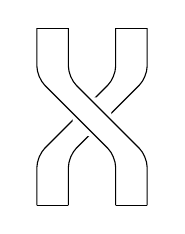
\begin{tikzpicture}[baseline]
				\node(xl1) at (-0.7,1){};
				\node(xr1) at (-0.3,1){};
				\node(yl1) at (0.3,1){};
				\node(yr1) at (0.7,1){};
				\node(yl2) at (-0.7, -1){};
				\node(yr2) at (-0.3, -1){};
				\node(xl2) at (0.3, -1){};
				\node(xr2) at (0.7, -1){};
				\node(b) at (0,0)[circle,fill=white, minimum size=0.5cm]{};
       				\draw[rounded corners](xl1.north) to (-0.7,0.5) to (0.3,-0.5) to (xl2.south);
       				\draw[rounded corners](xr1.north) to (-0.3,0.5) to (0.7,-0.5) to (xr2.south);
				\begin{pgfonlayer}{bg}
				\draw[rounded corners](yl1.north) to (0.3, 0.5) to (-0.7, -0.5) to (yl2.south);
				\draw[rounded corners](yr1.north) to (0.7, 0.5) to (-0.3, -0.5) to (yr2.south);
    				\end{pgfonlayer}
				\draw(xl1.north) to (xr1.north);
				\draw(xl2.south) to (xr2.south);
				\draw(yl1.north) to (yr1.north);
				\draw(yl2.south) to (yr2.south);
			\end{tikzpicture} & \quad \quad \quad \quad \quad \quad \quad &
			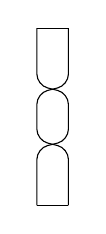
\begin{tikzpicture}[baseline]
				\node(xl1) at (-0.2,1){};
				\node(xr1) at (0.2,1){};	
				\node(xl2) at (-0.2, -1){};
				\node(xr2) at (0.2, -1){};
				\draw[rounded corners](xl1.north) to (-0.2,0.4) to (0.2, 0.3) to (0.2, -0.3) to (-0.2, -0.4) to (xl2.south);	
       				\draw[rounded corners](xr1.north) to (0.2,0.4) to (-0.2, 0.3) to (-0.2, -0.3) to (0.2, -0.4) to (xr2.south);
				\draw(xl1.north) to (xr1.north);
				\draw(xl2.south) to (xr2.south);	
			\end{tikzpicture} \\
			$b$ & & $t$ 
\end{tabular} \end{center}
This operad $RB$\index{action operad!of ribbon braid groups} is also clearly an action operad, since we can just define $\pi^{RB} : RB_{n} \to \mathrm{S}_n$ to act like $\pi^B$ on any braids, at which point the fact that $\pi(t) \in S_1 = \{e_1\}$ will automatically take care of the twists.

% \begin{example}
% \begin{enumerate}


% \item The operad of braid groups also has an obvious action operad structure in which the map $\pi$ is the group homomorphism sending a braid to its underlying permutation.  We will denote this action operad by $\mathbf{Br}$.  The operad of ribbon braids has an action operad structure, essentially using the same map $\pi$, and was studied by Wahl in \cite{wahl-thesis}.

% \end{enumerate}
% \end{example}

\begin{example}
Every abelian group $A$ gives rise to action operad $A^{\bullet}$\nomenclature[N]{$A^{\bullet}$}{action operad of an abelian group $A$}\index{action operad!of an abelian group} as follows.  The group $A^{\bullet}(n)$ is the direct sum of $n$ copies of $A$, $A^{n}$.  The identity element is required to be $e \in A^{1}$, and the multiplication is defined by
\[
\mu((a_{1}, \ldots, a_{n}); \mb{b_{1}}, \ldots, \mb{b_{n}}) = (a_{1}+\mb{b_{1}}, a_{2} + \mb{b_{2}}, \ldots, a_{n} + \mb{b_{n}})
\]
where $\mb{b_{i}}$ is the string $b_{i1}, \ldots, b_{in_{i}}$, and $a_{i} + \mb{b_{i}}$ is
\[
a_{i} + b_{i1}, a_{i} + b_{i2}, \ldots, a_{i} + b_{in_{i}}.
\]
\end{example}


Action operads are themselves the objects of a category, $\mb{AOp}$\nomenclature[C]{$\mb{AOp}$}{of action operads and maps of action operads}.  The morphisms of this category are defined below.
\begin{Defi}\label{mapaop}
A \textit{map of action operads}\index{action operad!maps} $f: \ML \rightarrow \ML'$ consists of a map $f:\Lambda \rightarrow \Lambda'$ of the underlying operads such that
\begin{enumerate}
\item $\pi^{\Lambda'} \circ f = \pi^{\Lambda}$ (i.e., $f$ is a map of operads over $\Sigma$) and
\item each $f_{n}:\Lambda(n) \rightarrow \Lambda'(n)$ is a group homomorphism.
\end{enumerate}
\end{Defi}

\begin{Defi}\label{Defi:cat_aop}
The category $\mb{AOp}$\index{action operad!category of} of action operads has objects which are action operads $\mb{\Lambda}$ and
 morphisms $\mb{\Lambda} \rightarrow \mb{\Lambda'}$ as defined in \cref{mapaop}.
\end{Defi}

\section{Some algebra in action operads}
Here we describe a host of useful results about action operads, including a characterisation of action operads via algebra involving the groups $\Lambda(n)$.

We begin with a simple proposition.

\begin{prop}
The map $\pi:\ML \to \mb{\Sigma}$ is a map of action operads.
\end{prop}


\begin{prop}\label{Z}
There is a functor $Z: \mb{Op}(\mb{Grp}) \to \mb{AOp}$\nomenclature[C]{$\mb{Op}(\mb{Grp})$}{of operads in groups and maps of operads in groups} from the category of operads in groups (using the cartesian monoidal structure) to the category of action operads.  This functor is full, faithful, and its image is precisely the collection of action operads $\ML$ with $\pi_{n}(g) = e_{n}$ for all $n, g \in \Lambda(n)$.
\end{prop}
\begin{proof}
Given an operad in groups $P$, $Z(P)$ is the action operad with the same underlying operad and each $\pi_{n}$ the zero map.  It is easy to verify that $\mu$ is a group homomorphism if and only if $\pi_{n}$ is zero for all $n$, and further that maps between such action operads are precisely the same thing as maps between the corresponding operads in the category of groups.
\end{proof}

We have the following corollary.
\begin{cor}\label{corZ}
For an action operad $\ML$, the sets\index{action operad!kernel}
\[
\textrm{Ker}\,\pi(n) = \{g \in \Lambda(n) : \pi_{n}(g) = e_{n} \}
\]
form an action operad for which the inclusion $\textrm{Ker}\,\pi \hookrightarrow \Lambda$ is a map of action operads.
\end{cor}
\begin{proof}
For $\textrm{Ker}\,\pi \hookrightarrow \Lambda$ to be a map of action operads, we must define the map $\textrm{Ker}\,\pi \rightarrow \Sigma$ to be zero,  and we must check that the operadic multiplication of elements in the kernel is also in the kernel.  This last fact is a trivial consequence of $\pi$ being an operad map.
\end{proof}

%\begin{rem}
%Zhang shows in Corollary 2.17 of \cite{zhang-grp} that the maps $\pi$ are either all zero or all surjective.  In particular, we now see that every action operad is either an operad in the category groups or an extension of $\Sigma$ by such an operad.  This gives a simple proof that the operads of pure braids and pure ribbon braids are both operads in groups.
%\end{rem}


\begin{prop}[Corollary 2.17,  \cite{zhang-grp}]\label{zero/surj}
The homomorphisms $\pi_n : \Lambda_n \to \Sigma_n$ are either all surjective or all the zero map.
\end{prop}

\begin{cor}\label{extension}
Every action operad $\ML$ with nontrivial $\pi$ fits into a short exact sequence
\[
T \to \textrm{Ker}\,\pi \hookrightarrow \Lambda \stackrel{\pi}{\longrightarrow} \Sigma \to T,
\]
by which we mean this is a sequence of action operad maps which is an exact sequence of groups at each $n$.
\end{cor}

\begin{rem}
Thus we see that an action operad is either an operad in groups, or is an extension of $\Sigma$ by an operad in groups.
\end{rem}

\begin{rem}
The crossed simplicial groups\index{crossed simplicial group} of Fiedoriwicz and Loday \cite{FL91} are related to action operads in the following way. There is a functor $C \colon \mathbf{AOp} \rightarrow \mathbf{CSGrp}$\nomenclature[C]{$\mathbf{CSGrp}$}{of crossed simplicial groups and morphisms of crossed simplicial groups} from the category of action operads just described into the category of crossed simplicial groups. This functor takes an action operad $\ML$ and defines $C(\Lambda)(n) = \Lambda_{n+1}$. The face and degeneracy maps of the underlying simplicial structure are defined using the operadic composition inherent of $\Lambda$ - the description of the maps via the operad structure can be viewed in a similar way to Construction 1.1 of \cite{Kra96}. This functor is, however, not faithful, nor is it conservative.
\end{rem}
%Salvatore-Wahl:  Framed disks operads...

\begin{lem}\label{calclem}
Let $\ML$ be an action operad, and write $e_{n}$ for the unit element in the group $\Lambda(n)$.
\begin{enumerate}
\item In $\Lambda(1)$, the unit element $e_{1}$ for the group structure is equal to the identity element for the operad structure, $\textrm{id}$.
\item The equation
\[
\mu(e_{n}; e_{i_{1}}, \ldots, e_{i_{n}}) = e_{I}
\]
holds for any natural numbers $n, i_{j}, I = \sum i_{j}$.
\item The group $\Lambda(1)$ is abelian.
\end{enumerate}
\end{lem}
\begin{proof}
For the first claim, let $g \in \Lambda(1)$.  Then
\[
\begin{array}{rcl}
g & = & g \cdot e_{1} \\
& = & \mu(g; \textrm{id}) \cdot \mu(\textrm{id}; e_{1}) \\
& = & \mu(g \cdot \textrm{id}; \textrm{id} \cdot e_{1}) \\
& = & \mu(g \cdot \textrm{id}; \textrm{id}) \\
& = & g \cdot \textrm{id}
\end{array}
\]
using that $e_{1}$ is the unit element for the group structure, that $\textrm{id}$ is a two-sided unit for operad multiplication, and the final axiom for an action operad together with the fact that the only element of the symmetric group $\Sigma_{1}$ is the identity permutation.  Thus $g = g \cdot \textrm{id}$, so $\textrm{id} = e_{1}$.

For the second claim, write the operadic product as $\mu(e; \underline{e})$, and consider the square of this element. We have
\[
\begin{array}{rcl}
\mu(e; \underline{e}) \cdot \mu(e; \underline{e}) & = & \mu(e \cdot e; \underline{e} \cdot \underline{e}) \\
&= & \mu(e; \underline{e})
\end{array}
\]
where the first equality follows from the last action operad axiom together with the fact that $e$ gets mapped to the identity permutation; here $\underline{e} \cdot \underline{e}$ is the sequence $e_{i_{1}} \cdot e_{i_{1}}, \ldots, e_{i_{n}} \cdot e_{i_{n}}$.  Thus $\mu(e; \underline{e})$ is an idempotent element of the group $\Lambda(I)$, so must be the identity element $e_{I}$.

For the final claim, note that operadic multiplication $\mu:\Lambda(1) \times \Lambda(1) \rightarrow \Lambda(1)$ is a group homomorphism by the action operad axioms, and $\textrm{id} = e_{1}$ is a two-sided unit, so the Eckmann-Hilton argument shows that $\mu$ is actually group multiplication and that $\Lambda_{1}$ is abelian.
\end{proof}

Note that the operad of symmetric groups $\Sigma$ has its action operad structure determined by two auxiliary operations.  The first is the block sum of permutations which we denote by
\[
\beta: \Sigma_{k_{1}} \times \cdots \times \Sigma_{k_{n}} \rightarrow \Sigma_{\underline{k}},
\]
where $\underline{k} = \sum k_{i}$.  The second is a kind of diagonal map which is defined for any natural number $n$ together with natural numbers $k_{1}, \ldots, k_{n}$.  Then
\[
\delta = \delta_{n; k_{1}, \ldots, k_{n}}:\Sigma_{n} \rightarrow \Sigma_{\underline{k}},
\]
is defined on $\sigma \in \Sigma_{n}$ by permuting the elements $1, 2, \ldots, k_{1}$ together in a block according to the action of $\sigma \in \Sigma_{n}$ on $1$, then $k_{1}+1, \ldots, k_{1}+k_{2}$ together in a block according to the action of $\sigma$ on $2$, and so on.  The first of these, $\beta$, is a group homomorphism, while $\delta$ QQQ put these in the notation index? is a sort of twisted homomorphism, and taken together they define operadic multiplication in $\Sigma$.  We now use these ideas to give the following algebraic characterization of action operads via the following definition.

\begin{Defi}\label{Defi:aop_bl}
For an action operad $\mb{\Lambda}$,  define
\[
\begin{array}{rcl}
\beta(h_{1}, \ldots, h_{n}) &=& \mu(e; h_{1}, \ldots, h_{n}) \\
\delta(g) &=& \mu(g; e_{1}, \ldots, e_{n}).
\end{array}
\]
\end{Defi}

\begin{nota}
We will denote our identity elements in groups generically as $e$. If $\{ G_{i} \}_{i \in I}$ are groups indexed by a set $I$, then $e_{i}$ is the identity element in $G_{i}$.
\end{nota}

\begin{thm}\label{thm:charAOp}
An action operad $\mb{\Lambda}$ determines, and is determined by, the following:
\begin{itemize}
\item groups $\Lambda(n)$ together with group homomorphisms $\pi_{n}:\Lambda(n) \rightarrow \Sigma_{n}$,
\item a group homomorphism
\[
\begin{array}{rcl}
\Lambda(k_{1}) \times \cdots \times \Lambda(k_{n}) & \stackrel{\beta}{\longrightarrow} & \Lambda(k_{1} + \cdots + k_{n}),
\end{array}
\]
for each $k_{1}, \ldots, k_{n}$ together with the degenerate case of $n=0$ which then is a group homomorphism $1 \to \Lambda(0)$, and
\item a function of sets
\[
\begin{array}{rcl}
\Lambda(n) & \stackrel{\delta_{n; k_{1}, \ldots, k_{n}}}{\longrightarrow} & \Lambda(k_{1} + \cdots + k_{n})
\end{array}
\]
for each $n, k_{1}, \ldots, k_{n}$,
\end{itemize}
subject to the axioms below.  In what we write below, we use the following notational conventions.
\begin{itemize}
\item The symbols $f,g,h$, with or without subscripts, always refer to an element of some group $\Lambda(n)$.
\item The symbols $j,k,m,n,p$ are all natural numbers, and $i$ is a natural number between 1 and $n$.
\end{itemize}
Axioms:
\begin{enumerate}
\item\label{eq1} The homomorphisms $\beta$ are natural with respect to the maps $\pi_{n}$, where $\underline{k} = k_{1} + \cdots + k_{n}$.
\[
\xy
% var defs
% 00    20
% 01    21
%    12(end)
(0,0)*+{\Lambda(k_{1}) \times \cdots \times \Lambda(k_{n}) } ="00";
(0,-15)*+{\Sigma_{k_{1}} \times \cdots \times \Sigma_{k_{n}}  } ="01";
(40,0)*+{\Lambda(\underline{k}) } ="20";
(40,-15)*+{\Sigma_{\underline{k}} } ="21";
% diagram
{\ar^{\beta} "00" ; "20"};
{\ar^{\pi} "20" ; "21"};
{\ar_{\pi_1 \times \cdots \times \pi_n} "00" ; "01"};
{\ar_{\beta} "01" ; "21"};
\endxy
\]
\item\label{eq2} The homomorphism $\beta:\Lambda(k) \to \Lambda(k)$ is the identity.
\item\label{eq3} The homomorphisms $\beta$ are associative in the sense that
\[
\beta(h_{11}, \ldots, h_{1j_{1}}, h_{21}, \ldots, h_{2j_{2}}, \ldots, h_{nj_{n}}) = \beta\big( \beta(h_{11}, \ldots, h_{1j_{1}}), \ldots, \beta(h_{n1}, \ldots, h_{nj_{n}}) \big)
\]
holds.
\item\label{eq4} The functions $\delta_{n; k_{1}, \ldots, k_{n}}$ are natural with respect to the maps $\pi_{n}$.
\[
\xy
% var defs
% 00    20
% 01    21
%    12(end)
(0,0)*+{\Lambda(n)} ="00";
(40,0)*+{\Lambda(k_{1} + \cdots + k_{n}) } ="20";
(0,-15)*+{\Sigma_{n}  } ="01";
(40,-15)*+{\Sigma_{k_{1} + \cdots + k_{n}} } ="21";
{\ar^{\delta} "00" ; "20"};
{\ar^{\pi} "20" ; "21"};
{\ar_{\pi} "00" ; "01"};
{\ar_{\delta} "01" ; "21"};
\endxy
\]
\item\label{eq5} The functions $\delta_{n; 1, \ldots, 1}, \, \delta_{1;n} : \Lambda(n) \to \Lambda(n)$ are the identity.
\item\label{eq6} The equation $\delta_{n; k_{i}}(g) \delta_{n; j_{i}}(h) = \delta_{n; j_{i}}(gh)$ holds when
\[
k_{i} = j_{\pi(h)^{-1}(i)}.
\]
\item\label{eq7} The functions $\delta$ are associative in the sense that
\[
\delta_{m_1 + \cdots + m_n; p_{11}, \ldots, p_{1m_{1}}, p_{21}, \ldots, p_{nm_{n}}}\big( \delta_{n; m_{1}, \ldots, m_{n}}(f) \big) = \delta_{n; P_{1}, \ldots, P_{n}}(f)
\]
where $P_{i} = p_{i1} + \cdots + p_{im_{i}}$.
\item\label{eq8} $\delta(g) \beta(h_{1}, \ldots, h_{n}) = \beta(h_{\pi(g)^{-1}(1)}, \ldots,  h_{\pi(g)^{-1}(n)}) \delta(g)$, where $h_{i} \in \Lambda(k_{i})$ and $\delta:\Lambda(n) \rightarrow \Lambda(k_{1} + \cdots + k_{n})$.
\item\label{eq9} The equation
\[
\beta(\delta_{1}(g_{1}), \ldots, \delta_{n}(g_{n})) = \delta_{c}(\beta(g_{1}, \ldots, g_{n}))
\]
holds, where $\delta_{i}(g_{i})$ is shorthand for $\delta_{k_{i}; m_{i1}, \ldots, m_{ik_{i}}}(g_{i})$ and $\delta_{c}$ is shorthand for
\[
\delta_{k_{1}+\cdots + k_{n}; m_{11}, m_{12}, \ldots, m_{1k_{1}}, m_{21}, \ldots, m_{nk_{n}}}.
\]
\end{enumerate}
\end{thm}

\begin{proof}
Let $\mb{\Lambda}$ be an action operad, and define $\beta, \delta$ as in \cref{Defi:aop_bl}.  Since $\pi:\Lambda \rightarrow \Sigma$ is an operad map, axioms \eqref{eq1} and \eqref{eq4} hold.  Since $\Lambda$ is an operad of sets, axioms \eqref{eq2} and \eqref{eq5} follow from the operad unit axioms, and axioms \eqref{eq3}, \eqref{eq7}, and \eqref{eq9} follow from the operad associativity axiom.  Axioms \eqref{eq6} and \eqref{eq8} are special cases of the additional action operad axiom, as is the fact that $\beta$ is a group homomorphism.

Given the data above, we need only define the operad multiplication, verify the operad unit and multiplication axioms,  and finally check the action operad axiom.  Multiplication is given by
\[
\mu(g; h_{1}, \ldots, h_{n}) = \delta_{n; k_{1}, \ldots, k_{n}}(g) \beta(h_{1}, \ldots, h_{n})
\]
where $h_{i} \in \Lambda(k_{i})$.  The unit is $e \in \Lambda(1)$.

We now verify the operad unit axioms.
\[
\begin{array}{rcl}
\mu(e; g) & = & \delta(e)\beta(g) \\
& = & e \cdot g \\
& = & g
\end{array}
\]
\[
\begin{array}{rcl}
\mu(h; e, \ldots, e) & = & \delta(h)\beta(e, \ldots, e) \\
& = & h \cdot e \\
& = & h
\end{array}
\]
These follow from axioms \eqref{eq2} and \eqref{eq5}, together with the fact that $\beta$ is a group homomorphism.

For the operad associativity axiom, let
\begin{itemize}
\item $f \in \Lambda(m),$
\item $g_{i} \in \Lambda(n_{i})$ for $i=1, \ldots, m$, and
\item $h_{ij} \in \Lambda(p_{i,j})$ for $i=1, \ldots, m$ and $j=1, \ldots, n_{i}$.
\end{itemize}
Further, let $P_{i} = p_{i1} + \cdots + p_{in_{i}}$ and $\underline{h_{i\bullet}}$ denote the list $h_{i1}, h_{i2}, \ldots, h_{in_{i}}$.  We must then show that
\[
\mu\big( f; \mu(g_{1}; \underline{h_{1\bullet}}), \ldots, \mu(g_{m}; \underline{h_{m\bullet}}) \big) = \mu\big( \mu (f; g_{1}, \ldots, g_{m}); h_{11}, \ldots, h_{1n_{1}}, h_{21}, \ldots, h_{mn_{m}} \big).
\]
By definition, the left side of this equation is
\[
\delta_{m; P_{1}, \ldots, P_{m}}(f) \beta\big( \mu(g_{1}; \underline{h_{1\bullet}}), \ldots, \mu(g_{m}; \underline{h_{m\bullet}}) \big),
\]
and
\[
\mu(g_{i}; \underline{h_{i\bullet}}) = \delta_{n_{i}; p_{i1}, \ldots, p_{in_{i}}}(g_{i})\beta(h_{i1}, \ldots, h_{in_{i}}).
\]
Since $\beta$ is a group homomorphism, we can then rewrite the left side as
\[
\delta(f)\beta\big(\delta(g_{1}), \ldots, \delta(g_{m})\big)\beta\big(\beta(h_{1\bullet}), \ldots, \beta(h_{m\bullet})\big)
\]
where we have suppressed the subscripts on the $\delta$'s.  By axiom \eqref{eq3} , we have
\[
\beta\big(\beta(h_{1\bullet}), \ldots, \beta(h_{m\bullet})\big) = \beta(h_{11}, \ldots, h_{1n_{1}}, h_{21}, \ldots, h_{mn_{m}}).
\]
Further, axiom \eqref{eq9} above shows that
\[
\beta\big(\delta(g_{1}), \ldots, \delta(g_{m})\big) = \delta\big(\beta(g_{1}, \ldots, g_{m})\big).
\]
Thus we have shown that the left side of the operad associativity axiom is equal to
\[
\delta(f)\delta\big(\beta(g_{1}, \ldots, g_{m})\big)\beta(h_{11}, \ldots, h_{1n_{1}}, h_{21}, \ldots, h_{mn_{m}}).
\]
Now the right side is
\[
\mu\big( \mu (f; g_{1}, \ldots, g_{m}); h_{11}, \ldots, h_{1n_{1}}, h_{21}, \ldots, h_{mn_{m}} \big)
\]
which is by definition
\[
\delta\big(\mu (f; g_{1}, \ldots, g_{m})\big)\beta(h_{11}, \ldots, h_{1n_{1}}, h_{21}, \ldots, h_{mn_{m}} ).
\]
Thus verifying the operad associativity axiom reduces to showing
\begin{eqn}\label{eqn:opass}
\delta(f)\delta\big(\beta(g_{1}, \ldots, g_{m})\big) = \delta\big(\mu (f; g_{1}, \ldots, g_{m})\big).
\end{eqn}By the definition of $\mu$, we have
\[
\delta(\mu (f; g_{1}, \ldots, g_{m})) = \delta\big(\delta(f)\beta(g_{1}, \ldots, g_{m}) \big)
\]
which is itself equal to
\begin{eqn}\label{eqn:opass2}
\delta\big(\delta(f)\big) \delta\big(\beta(g_{1}, \ldots, g_{m})\big)
\end{eqn}by axiom \eqref{eq6} above.  Now the $\delta(f)$ on the left side of \cref{eqn:opass} uses $\delta_{n; P_{1}, \ldots, P_{n}}$, while the $\delta(\delta(f))$ in \cref{eqn:opass2} is actually
\[
\delta_{m_1 + \cdots + m_{n}; q_{ij}}(\delta_{n; m_{1}, \ldots, m_{n}} (f))
\]
where the $q_{ij}$ are defined, by axiom \eqref{eq6}, to be given by
\[
q_{ij} = p_{i,\pi(g_{i})^{-1}(j)}
\]
using the compatibility of $\beta$ and $\pi$ in axiom \eqref{eq1}.  By axiom \eqref{eq7}, this composite of $\delta$'s  is then $\delta_{n; Q_{1}, \ldots, Q_{n}}$ where $Q_{i} = q_{i1} + \cdots + q_{im_{i}}$.  But by the definition of the $q_{ij}$, we immediately see that $Q_{i} = P_{i}$, so the $\delta(f)$ in \cref{eqn:opass} is equal to the $\delta(\delta(f))$ appearing in \cref{eqn:opass2}, concluding the proof of the operad associativity axiom.

The action operad axiom is now the calculation below, and uses axioms \eqref{eq4} and \eqref{eq8}.
\begin{small}
\[
\begin{array}{rcl}
\mu(g; h_{1}, \ldots, h_{n})\mu(g'; h_{1}', \ldots, h_{n}') & = & \delta(g) \beta(h_{1}, \ldots, h_{n}) \delta(g') \beta(h_{1}', \ldots, h_{n}') \\
& = & \delta(g) \delta(g') \beta(h_{\pi(g')(1)}, \ldots, h_{\pi(g')(n)})  \beta(h_{1}', \ldots, h_{n}') \\
& = & \delta(gg') \beta(h_{\pi(g')(1)}h_{1}', \ldots, h_{\pi(g')(n)}h_{n}') \\
& = & \mu(gg'; h_{\pi(g')(1)}h_{1}', \ldots, h_{\pi(g')(n)}h_{n}')
\end{array}
\]
\end{small}
\end{proof}



\section{Presentations of action operads}\label{sec:presofacops}

One of the most useful methods for constructing new examples of some given algebraic structure is through the use of presentations.  A presentation consists of generating data together with relations between generators using the operations of the algebra involved.  In categorical terms, the generators  and relations are both given as free gadgets on some underlying data, and the presentation itself is a coequalizer.  This section will establish the categorical structure necessary to give presentations for action operads, and then explain how such a presentation is reflected in the associated club and 2-monad.  The most direct route to the desired results uses the theory of locally finitely presentable categories.  We recall the main definitions briefly, but refer the reader to \cite{ar} for additional details.

QQQ Do we use any of these definitions? We seem to need to know the following things about locally finitely presentable categories:
	\begin{itemize}
		\item That any presheaf category is lfp.
		\item That $\bf{Cat}$ is lfp.
		\item That if $\m{C}$ is lfp and $X \in \m{C}$, then the slice category $\m{C}/X$ is lfp.
		\item That a category which is an equational theory with only finitely many elements is lfp.
	\end{itemize}
These should all be simple facts following from Adamek/Rosicky (AR), except maybe the last one which I think is just a case of awkward wording. Maybe we should take the definitions out and just refer to AR? QQQ

\begin{Defi}
A \textit{filtered category}\index{category!filtered} is a nonempty category $C$ such that
\begin{itemize}
\item if $a,b$ are objects of $C$, then there is another object $c \in C$ and morphisms $a \to c, b \to c$; and
\item if $f,g \cn a \to b$ are parallel morphisms in $C$, then there exists a morphism $h \cn b \to c$ such that $hf = hg$.
\end{itemize}
\end{Defi}

\begin{Defi}
A \emph{filtered colimit}\index{colimit!filtered} is a colimit over a filtered category.
\end{Defi}

\begin{Defi}
Let $C$ be a category with all filtered colimits.  An object $x \in C$ is \textit{finitely presentable}\index{object!finitely presentable} if the representable functor $C(x, -):C \rightarrow \mb{Sets}$ preserves filtered colimits.
\end{Defi}

\begin{Defi}
A \textit{locally finitely presentable category}\index{category!locally finitely presentable} is a category $C$ such that
\begin{itemize}
\item $C$ is cocomplete and
\item there exists a small subcategory $C_{fp}\nomenclature[C]{$C_{fp}$}{the subcategory of finitely presentable objects in $C$} \subseteq C$ of finitely presentable objects such that any object $x \in C$ is the filtered colimit of some diagram in $C_{fp}$.
\end{itemize}
\end{Defi}

The definition of a locally finitely presentable category has many equivalent variants, and our applications are quite straightforward so we have given what is probably the most common version of the definition.  We refer the reader to \cite{ar} for more information.  The following result will be clear to the experts, so we just sketch a proof. QQQ Too informal.


\begin{thm}
The category $\mb{AOp}$ is locally finitely presentable.
\end{thm}
\begin{proof}
$\mb{Op}^{g}$\nomenclature[C]{$\mb{Op}^{g}$}{of operads $P$ for which each $P(n)$ has a group structure and operad maps} whose objects are operads $P$ in which each $P(n)$ also carries a group structure. This is an equational theory using equations with only finitely many elements, so $\mb{Op}^{g}$ is locally finitely presentable. QQQ Reference? (Adamek and Rosicky?) The symmetric operad is an object of this category, so the slice category\index{category!slice category} $\mb{Op}^{g}/\Sigma$ is also locally finitely presentable.  There is an obvious inclusion functor $\mb{AOp} \hookrightarrow \mb{Op}^{g}/\Sigma$.  Now $\mb{AOp}$ is a full subcategory of $\mb{Op}^{g}/\Sigma$ which is closed under products, subobjects, and any object of $\mb{Op}^{g}/\Sigma$ isomorphic to an action operad is in fact an action operad, so the inclusion   $\mb{AOp} \hookrightarrow \mb{Op}^{g}/\Sigma$ is actually the inclusion of a reflective subcategory.  One easily checks that $\mb{AOp}$ is in fact closed under all limits and filtered colimits in $\mb{Op}^{g}/\Sigma$, so by the Reflection Theorem (2.48 in \cite{ar}), $\mb{AOp}$ is locally finitely presentable.
\end{proof}

\begin{Defi}
Let $\SS$ be the set which is the disjoint union of the underlying sets of all the symmetric groups.  Then $\mb{Sets}/\SS$ is the slice category over $\SS$ with objects $(X,f)$ where $X$ is a set and $f:X \rightarrow \SS$ and morphisms $(X_{1}, f_{1}) \rightarrow (X_{2}, f_{2})$ are those functions $g:X_{1} \rightarrow X_{2}$ such that $f_{1} = f_{2}g$.  We call an object $(X,f)$ a \textit{collection over $\SS$}.
\end{Defi}

\begin{rem}
In standard presentations of the theory of operads (see, for example, \cite{mss-op}), a nonsymmetric operad will have an underlying collection\index{collection!non-symmetric} (or $\mathbb{N}$-indexed collection of sets) while a symmetric operad will have an underlying symmetric collection\index{collection!symmetric} (or $\mathbb{N}$-indexed collection of sets in which the $n$th set has an action of $\Sigma_{n}$).  Our collections over $\SS$ more closely resemble the former as there is no group action present.
%an action operad is \textit{a priori} a nonsymmetric operad with some extra structure.  Part of that structure is the notion of the underlying permutation of an element $g \in \Lambda(n)$, and a collection over $\SS$ keeps track of all the underlying permutations separately.  To recover a notion of collection akin to that for symmetric operads, we should define $X(n)$ to be the preimage of all $\sigma \in \Sigma_{n}$ under $f:X \rightarrow \SS$.
\end{rem}

\begin{example}
One can easily form new action operads from old ones by taking limits\index{action operad!limits of}.  To take a limit of a diagram in $\mb{AOp}$, one forgets down to the category of operads over $\Sigma$ and takes the limit there.  Concretely, products in $\mb{AOp}$ are computed as products in $\mb{Op}/\Sigma$\nomenclature[C]{$C/c$}{the slice category of $C$ over an object $c$ in $C$} (see QQQ) which themselves are (possibly wide) pullbacks in the category of operads.  This pullback will then be computed levelwise, showing that at each dimension we have a group structure with a group homomorphism to the appropriate $\Sigma_{n}$ and that the final action operad axiom holds since it does in each component.  The equalizer of a pair of maps will then just be the levelwise equalizer.  This shows that the pointwise product of an action operad $P$ with an action operad of the form $Z(Q)$ is again an action operad, but the pointwise product of two arbitrary action operads might not be.
\end{example}
\begin{thm}\label{underlyingSS}
There is a forgetful functor $U:\mb{AOp} \rightarrow \mb{Sets}/\SS$ which preserves all limits and filtered colimits.
\end{thm}

\begin{proof}
The functor $U$ is obvious, and the preservation of filtered colimits follows from the fact that these are computed pointwise, together with the fact that every map between action operads preserves underlying permutations.
% For limits, recall that limits in $\mb{AOp}$ are computed as in the category of operads over $\Sigma$.
% This means that equalizers are computed levelwise, and the product $\mb{\Lambda} \times \mb{\Lambda}'$ has underlying operad the pullback $\Lambda \times_{\Sigma} \Lambda'$; this pullback is itself computed levelwise.  Together, these imply that $U$ also preserves all limits.
As equalizers are computed levelwise, and the product $\mb{\Lambda} \times \mb{\Lambda}'$ has underlying operad the pullback $\Lambda \times_{\Sigma} \Lambda'$; this pullback is itself computed levelwise.  Together, these imply that $U$ also preserves all limits.
\end{proof}

\begin{cor}
$U$ has a left adjoint $F:\mb{Sets}/\SS \rightarrow \mb{AOp}$, the free action operad functor.
\end{cor}
\begin{proof}
The category $\mb{Sets}/\SS$ is locally finitely presentable as it is equivalent to the functor category $[\SS, \mb{Sets}]$\nomenclature[C]{$[A,B]$}{of functors between categories $A$ and $B$ and natural transformations} (here $\SS$ is treated as a discrete category) and any presheaf category is locally finitely presentable.  The functor $U$ preserves limits and filtered colimits between locally finitely presentable categories, so has a left adjoint (see Theorem 1.66 in \cite{ar}).
\end{proof}

\begin{Defi}
A \textit{presentation}\index{action operad!presentation} for an action operad $\mb{\Lambda}$ consists of
\begin{itemize}
\item a pair of collections over $\SS$ denoted $\mathbf{g}, \mathbf{r}$,
\item a pair of maps $s_{1}, s_{2}:F\mathbf{r} \rightarrow F\mathbf{g}$ between the associated free action operads, and
\item a map $p:F\mathbf{g} \rightarrow \mb{\Lambda}$ of action operads exhibiting $\mb{\Lambda}$ as the coequalizer of $s_{1},s_{2}$.
\end{itemize}
\end{Defi}









\section{Operads and algebras with general group actions}
Just as we had the definitions of operad, symmetric operad, and braided operad, we now come to the general definition of a $\ML$-operad, where $\ML$ is an action operad.

\begin{Defi}\label{Defi:lamop}
Let $\ML$ be an action operad.  A \textit{$\ML$-operad}\index{operad!$\ML$-operad} $P$ (in $\mb{Sets}$) consists of
\begin{itemize}
\item a non-symmetric operad $P$ in $\mb{Sets}$ and
\item for each $n$, an action $P(n) \times \Lambda(n) \rightarrow P(n)$ of $\Lambda(n)$ on $P(n)$
\end{itemize}
such that the following two equivariance axioms hold.
\[
\begin{array}{c}
\mu^{P}(x; y_{1} \cdot g_{1}, \ldots, y_{n} \cdot g_{n}) =\mu^{P}(x; y_{1}, \ldots, y_{n}) \cdot \mu^{\Lambda}(e; g_{1}, \ldots, g_{n})  \\
\mu^{P}(x \cdot g; y_{1}, \ldots, y_{n})  =  \mu^{P}(x; y_{\pi(g)^{-1}(1)}, \ldots, y_{\pi(g)^{-1}(n)}) \cdot \mu^{\Lambda}(g; e_{1}, \ldots, e_{n})
\end{array}
\]
\end{Defi}

\begin{Defi}
The category $\ML\mbox{-}\mb{Op}$\nomenclature[C]{$\ML\mbox{-}\mb{Op}$}{of $\Lambda$-operads and maps of operads which are levelwise equivariant with respect to the $\Lambda(n)$-actions}\index{operad!$\ML$-operad!category of} of $\Lambda$-operads has objects the $\ML$-operads and morphisms those maps of operads which are levelwise equivariant with respect to the $\Lambda(n)$-actions.
\end{Defi}

\begin{example}
\begin{enumerate}
\item Let $\mb{T}$\index{action operad!initial}\index{operad!terminal} denote the terminal operad in $\mb{Sets}$ equipped with its unique action operad structure.  Then a $\mb{T}$-operad is just a non-symmetric operad in $\mb{Sets}$.
\item Let $\mb{\Sigma}$\index{operad!of symmetric groups} denote the operad of symmetric groups with $\pi:\Sigma \rightarrow \Sigma$ the identity map.  Then a $\mb{\Sigma}$-operad is a symmetric operad in the category of sets.
\item Let $\mb{B}$\index{operad!of braid groups} denote the operad of braid groups with $\pi_{n}:B_{n} \rightarrow \Sigma_{n}$ the canonical projection of a braid onto its underlying permutation.  Then a $\mb{B}$-operad is a braided operad in the sense of Fiedorowicz \cite{fie-br}.
\end{enumerate}
\end{example}

A further example of a $\ML$-operad is given by the underlying operad, $\Lambda$, of $\ML$ itself.
\begin{prop}\label{gisgop}
Let $\mb{\Lambda}$ be an action operad.  Then the operad $\Lambda$ is itself a $\mb{\Lambda}$-operad.
\end{prop}
\begin{proof}
The underlying operad $\Lambda$ is of course an operad in $\mb{Sets}$. The action $\Lambda(n) \times \Lambda(n) \rightarrow \Lambda(n)$ is given simply by the group multiplication in $\Lambda(n)$. The two equivariance axioms are then both instances of the action operad axiom of $\ML$.
\end{proof}

An operad is intended to be an abstract description of a certain type of algebraic structure, and the particular instances of that structure are the algebras for that operad.  We begin with the definition of an algebra over a non-symmetric operad and add in the group actions later.

\begin{Defi}\label{opalgax}
Let $O$ be a non-symmetric operad.  An \textit{algebra}\index{algebra!operad}\index{operad!algebra} for $O$ consists of a set $X$ together with maps $\alpha_{n}:O(n) \times X^{n} \rightarrow X$ such that the following axioms hold.
\begin{enumerate}
\item The element $\textrm{id} \in O(1)$ is a unit in the sense that
\[
\alpha_{1}(\textrm{id}; x) = x
\]
for all $x \in X$.
\item The maps $\alpha_{n}$ are associative in the sense that the diagram
\[
\xy
(0,0)*+{O(n) \times O(k_{1}) \times X^{k_{1}} \times \cdots \times O(k_{n}) \times X^{k_{n}}}="ul";
(75,0)*+{O(n) \times X^{n}}="ur";
(0,-12)*+{O(n) \times O(k_{1}) \times \cdots \times O(k_{n}) \times X^{k_{1}} \times \cdots \times X^{k_{n}}}="ml";
(0,-24)*+{O(\sum k_{i}) \times X^{\sum k_{i}}}="bl";
(75,-24)*+{X}="br";
{\ar^>>>>>>>>>>>>>>{1 \times \alpha_{k_{1}} \times \cdots \alpha_{k_{n}}} "ul"; "ur"};
{\ar^{\alpha_{n}} "ur"; "br"};
{\ar_{\cong} "ul"; "ml"};
{\ar_{\mu \times 1} "ml"; "bl"};
{\ar_{\alpha_{\sum k_{i}}} "bl"; "br"};
\endxy
\]
commutes.
\end{enumerate}
\end{Defi}


Moving on to algebras for a $\ML$-operad, let $P$ be a $\ML$-operad and let $X$ be any set.  Write $P(n) \times_{\Lambda(n)} X^{n}$ for the coequalizer of the pair of maps
\[
P(n) \times \Lambda(n) \times X^{n} \rightrightarrows P(n) \times X^{n}
\]
of which the first map is the action of $\Lambda(n)$ on $P(n)$ and the second map is
\[
P(n) \times \Lambda(n) \times X^{n} \rightarrow P(n) \times \Sigma_{n} \times X^{n} \rightarrow P(n) \times X^{n}
\]
using $\pi_{n}:\Lambda(n) \rightarrow \Sigma_{n}$ together with the canonical action of $\Sigma_{n}$ on $X^{n}$ by permutation of coordinates: $\sigma \cdot (x_{1}, \ldots, x_{n}) = (x_{\sigma^{-1}(1)}, \ldots, x_{\sigma^{-1}(n)})$.  By the universal property of the coequalizer, a function $f:P(n) \times_{\Lambda(n)} X^{n} \rightarrow Y$ can be identified with a function $\tilde{f}:P(n) \times X^{n} \rightarrow Y$ such that
\[
\tilde{f}(p\cdot g; x_{1}, \ldots, x_{n}) = \tilde{f}(p; x_{\pi(g)^{-1}(1)}, \ldots, x_{\pi(g)^{-1}(n)}).
\]

\begin{Defi}
Let $P$ be a $\Lambda$-operad.  An \textit{algebra}\index{algebra!$\Lambda$-operad} for $P$ consists of a set $X$ together with maps $\alpha_{n}:P(n) \times_{\Lambda(n)} X^{n} \rightarrow X$ such that the maps $\tilde{\alpha}_{n}$ satisfy the operad algebra axioms given in Definition \ref{opalgax}.
\end{Defi}

\begin{rem}
It is worth noting that the equivariance required for a $P$-algebra is built into the definition above by requiring the existence of the maps $\alpha_{n}$ to be defined on coequalizers, even though the algebra axioms then only use the maps $\tilde{\alpha}_{n}$.  Since every $\ML$-operad has an underlying plain operad (see \ref{pbaop}, applied to the unique map $\mb{T} \rightarrow \ML$), this reflects the fact that the algebras for the $\ML$-equivariant version are always algebras for the plain version, but not conversely.
\end{rem}

\begin{Defi}
The category of algebras\index{operad!algebra!category of} for $P$, $P\mbox{-}\mb{Alg}$\nomenclature[C]{$P\mbox{-}\mb{Alg}$}{of $P$-algebras and morphisms for an operad (or monad) $P$}, has objects the $P$-algebras $(X, \alpha)$ and morphisms $f: (X, \alpha) \rightarrow (Y, \beta)$ those functions $f:X \rightarrow Y$ such that the following diagram commutes for every $n$.
\[
\xy
{\ar^{1 \times f^{n}} (0,0)*+{P(n) \times X^{n}}; (50,0)*+{P(n) \times Y^{n}} };
{\ar^{\tilde{\beta}_{n}} (50,0)*+{P(n) \times Y^{n}}; (50,-15)*+{Y} };
{\ar_{\tilde{\alpha}_{n}} (0,0)*+{P(n) \times X^{n}}; (0,-15)*+{X} };
{\ar_{f} (0,-15)*+{X}; (50,-15)*+{Y} };
\endxy
\]
\end{Defi}

Let $X$ be a set.  Then the endomorphism operad of $X$, denoted $\mathcal{E}_{X}$\nomenclature[N]{$\mathcal{E}_{X}$}{the endomorphism operad of a set $X$}\index{operad!endomorphism operad}, is given by the sets $\mathcal{E}_{X}(n) = \mb{Sets}(X^{n}, X)$ with the identity function in $\mathcal{E}_{X}(1)$ giving the unit element and composition of functions giving the composition operation.  Concretely, composition is given by the formula
\[
\mu(f; g_{1}, \ldots, g_{n}) = f \circ (g_{1} \times \cdots \times g_{n}).
\]

\begin{lem}
Let $\ML$ be an action operad, and let $X$ be a set.  Then $\mathcal{E}_{X}$ carries a canonical $\ML$-operad structure.
\end{lem}
\begin{proof}
$\mathcal{E}_{X}$ is a symmetric operad, so we define the actions by
\[
\mathcal{E}_{X}(n) \times \Lambda(n) \stackrel{1 \times \pi_{n}}{\longrightarrow} \mathcal{E}_{X}(n) \times \Sigma_{n} \rightarrow \mathcal{E}_{X}.
\]
\end{proof}

The previous result is really a change-of-structure-groups result.  We record the general result as the following proposition.

\begin{prop}\label{pbaop}
Let $f:\ML \rightarrow \ML'$ be a map of action operads.  Then $f$ induces a functor $f^{*}:\Lambda'\mbox{-}\mb{Op} \to \Lambda\mbox{-}\mb{Op}$.
\end{prop}

We can now use endomorphism operads to characterize algebra structures.

\begin{prop}\label{endoalg}
Let $X$ be a set, and $P$ a $\ML$-operad.  Then algebra structures on $X$ are in 1-to-1 correspondence with $\ML$-operad maps $P \rightarrow \mathcal{E}_{X}$.
\end{prop}
\begin{proof}
A map $P(k) \rightarrow \mathcal{E}_{X}(k)$ corresponds, using the closed structure on $\mb{Sets}$, to a map $P(k) \times X^{k} \rightarrow X$.  The monoid homomorphism axioms give the unit and associativity axioms, and the requirement that $P \rightarrow \mathcal{E}_{X}$ be a map of $\ML$-operads gives the equivariance condition.
\end{proof}

\begin{rem}
The proposition above holds for $P$-algebras in any closed symmetric monoidal category.  Having a closed structure (in addition to all small colimits) is a stronger condition than the tensor preserving colimits in each variable, but it is a natural one that arises in many examples.
\end{rem}

\begin{Defi}
Let $P$ be a $\ML$-operad.  Then $P$ induces an endofunctor of $\mb{Sets}$, denoted $\underline{P}$\nomenclature[N]{$\underline{P}$}{the monad induced by an operad $P$}, by the following formula.
 \[
	\underline{P}(X)	 =  \coprod_n P(n) \times_{\Lambda(n)} X^n
\]
\end{Defi}

We now have the following proposition; its proof is standard \cite{maygeom}, and we leave it to the reader.

\begin{prop}\label{op=monad1}  Let $P$ be a $\ML$-operad.
\begin{enumerate}
\item The $\ML$-operad structure on $P$ induces a monad\index{monad}\index{operad!associated monad} structure on $\underbar{P}$.
\item The category of algebras for the operad $P$ is isomorphic to the category of algebras for the monad $\underbar{P}$.
\end{enumerate}
\end{prop}

In the case that we take $P = \Lambda$, we do not get algebras more interesting than monoids.
\begin{prop}
Let $\ML$ be an action operad. The category of algebras, $\Lambda\mbox{-}\mb{Alg}$, for $\Lambda$ taken as a $\ML$-operad, is equivalent to the category of monoids.
\end{prop}
\begin{proof}
The key observation here is that, for each $n \in \mathbb{N}$,
	\[
		\Lambda(n) \times_{\Lambda(n)} X^n \cong X^n.
	\]
We will describe this bijection and leave the rest of the proof to the reader, which falls out of the various axioms either for being a monoid or for being a $\ML$-algebra.

Recall that the elements of $\Lambda(n) \times_{\Lambda(n)} X^n$ are equivalence classes of the form $[g ; x_1, \ldots, x_n]$ for which
	\[
		(gh; x_1, \ldots, x_n) \sim (g; x_{\pi(h)^{-1}(1)}, \ldots, x_{\pi(h)^{-1}(n)}).
	\]
There is an obvious map $X^n \rightarrow \Lambda(n) \times_{\Lambda(n)} X^n$ sending $(x_1, \ldots, x_n)$ to the equivalence class $[e; x_1, \ldots, x_n]$. The inverse to this map is given by the map $\Lambda(n) \times_{\Lambda(n)} X^n \rightarrow X^n$ sending $[g;x_1,\ldots,x_n]$ to the element $(x_{\pi(g)^{-1}(1)},\ldots,x_{\pi(g)^{-1}(n)})$. It is then clear that these are inverses, relying on the equivalence relation to see that
	\[
		[g;x_1,\ldots,x_n] = [e;x_{\pi(g)^{-1}(1)},\ldots,x_{\pi(g)^{-1}(n)}].
	\]
That the second map is well-defined is simple to show.
\end{proof}

We end this section with a discussion of the relationship between symmetric operads and $\ML$-operads for an arbitrary action operad $\ML$.

\begin{thm}\label{thm_sym}
Let $\ML$ be an action operad.
\begin{enumerate}
\item There is an adjunction between the category of $\ML$-operads and the category of symmetric operads, with right adjoint $\pi^{*}:\ML\mbox{-}\mb{Op} \to \mb{\Sigma}\mbox{-}\mb{Op}$ and left adjoint denoted $S$.
\item The counit of this adjunction is an isomorphism, but the unit is not, thus this adjunction is not an equivalence of categories
\item There is a natural isomorphism of monads  between $\underline{P}$ and $\underline{S(P)}$ for a $\ML$-operad $P$.  In particular, these monads (and hence operads) have isomorphic categories of algebras.
\end{enumerate}
\end{thm}
\begin{proof}
Given any map of monoids $f:M \to N$ in a monoidal category, there is an adjunction between right $M$-modules and right $N$-modules given by $f^{*}$ as the right adjoint and $A \mapsto A \otimes_{M} N$ as the left adjoint.  Thus we define \[
S(P)(n) = P(n) \times_{\Lambda(n)} \Sigma_{n},
\]
and this inherits a right $\Sigma_{n}$-action by multiplication.  The unit of $S(P)$ is
\[
* \stackrel{\eta}{\longrightarrow} P(1) \longrightarrow P(1)\times_{\Lambda(1)}\Sigma_{1} \cong P(1)/\Lambda(1).
\]
For the multiplication, let $\underline{k} = k_1 + \cdots + k_n$, so we must define
\[
\mu: (P(n) \times_{\Lambda(n)} \Sigma_{n}) \times (P(k_1) \times_{\Lambda(k_1)} \Sigma_{k_1}) \times \cdots \times (P(k_n) \times_{\Lambda(k_n)} \Sigma_{k_n}) \to P(\underline{k}) \times_{\Lambda(\underline{k})} \Sigma_{\underline{k}}.
\]
Using the universal property of the coequalizer, this is induced by
\[
\begin{array}{rcl}
(P(n) \times \Sigma_{n}) \times (P(k_1) \times \Sigma_{k_1}) \times \cdots \times (P(k_n) \times \Sigma_{k_n}) & \cong & \\
 \Big(P(n) \times \prod P(k_{i}) \Big) \times \Big(\Sigma_{n} \times \prod \Sigma_{k_{i}} \Big) & \to &\\
   P(\underline{k}) \times \Sigma_{\underline{k}} & \to &  P(\underline{k}) \times_{\Lambda(\underline{k})} \Sigma_{\underline{k}}.
   \end{array}
\]
We leave verification of the associativity, unit, and equivariance axioms to the reader, they are simple applications of the same axioms for $P$ and $\Sigma$ together with some colimit universal properties and the $\ML$-operad axioms for $P$.  It is then straightforward to check the bijection between $\ML$-operad maps $P \to \pi^{*}Q$ and symmetric operad maps $S(P) \to Q$, thus establishing the adjunction.

The second claim is a simple calculation using the coequalizer that defines $S(\pi^{*}Q)$, using that $Q(n)$ is itself the coequalizer of the obvious pair of maps $Q(n) \times \Sigma_{n} \times \Sigma_{n}$.

For the third claim, we get a natural isomorphism
\[
P(n) \times_{\Lambda(n)}X^{n} \cong (P(n) \times_{\Lambda(n)} \Sigma_{n}) \times_{\Sigma_{n}} X^{n}
\]
by the universal property of the colimits involved, so as functors $\underline{P} \cong \underline{S(P)}$.  One can then easily verify that this isomorphism commutes with the unit and multiplication of the two monads involved using calculations similar to those used to establish the adjunction.
\end{proof}

\begin{rem}
\begin{enumerate}
\item The adjunction alone is enough to establish that $P$ and $S(P)$ have isomorphic categories of algebras using Proposition \ref{endoalg}.
\item This theorem shows that semantically, one need never consider any kind of operad aside from symmetric operads: any other kind of operad can be symmetrized without altering the algebras.  But as the operad should be considered a finer level of detail than the monad, restricting to symmetric operads misses the structure present in the more nuanced group actions.

\item Furthermore, there is clearly an artifact left from only considering the algebras themselves as objects in a symmetric monoidal category.  It is well-known that a braided structure is all that is required for non-symmetric operads, and so one is left to consider that the natural home for algebras over a $\ML$-operad might be a type of monoidal structure other than symmetric in which case the theorem above gives no insight.
\end{enumerate}
\end{rem}

We end this section by presenting some results which allow us to transfer operad or algebra structures to other categories. 

\begin{Defi}
Let $S$ be a monad on a category $C$ and $T$ be a monad on a category $D$. A \emph{monad map}\index{monad!maps} of from $S$ to $T$ is a functor $F : C \to D$ together with a natural transformation $\alpha:TF \Rightarrow FS$ such that the following diagrams commute.

 \[
    \xy
      (0,0)*+{FX}="a";
      (20,10)*+{TFX}="b";
      (20,-10)*+{FSX}="c";
      %
      {\ar^{\eta^T_{FX}} "a" ; "b"};
      {\ar^{\alpha_X} "b" ; "c"};
      {\ar_{F\eta^S_X} "a" ; "c"};
      %
      (40,0)*+{T^2FX}="a";
      (60,10)*+{TFSX}="b";
      (85,10)*+{FS^2X}="c";
      (60,-10)*+{TFX}="d";
      (85,-10)*+{FSX}="e";
      %
      {\ar^{T\alpha_X} "a" ; "b"};
      {\ar^{\alpha_{SX}} "b" ; "c"};
      {\ar^{F\mu^S_X} "c" ; "e"};
      {\ar_{\mu^T_{FX}} "a" ; "d"};
      {\ar_{\alpha_X} "d" ; "e"};
    \endxy
  \]
 
A \emph{transformation}\index{monad!maps!transformation} $\Gamma : (F, \alpha) \Rightarrow (G, \beta)$ is a natural transformation $\Gamma: F \Rightarrow G$ such that the following diagram commutes.
  
  \[
    \xy
      (0,0)*+{TFX}="a";
      (20,0)*+{TGX}="b";
      (0,-20)*+{FSX}="c";
      (20,-20)*+{GSX}="d";
      %
      {\ar_{\alpha_X} "a" ; "c"};
      {\ar_{\Gamma_{SX}} "c" ; "d"};
      {\ar^{T\Gamma_X} "a" ; "b"};
      {\ar^{\beta_X} "b" ; "d"};
    \endxy
  \]
\end{Defi}

Every monad map $(F,\alpha)$ induces a functor $S\Alg \rightarrow T\Alg$ on the categories of algebras. An $S$-algebra $(X,\sigma)$ is sent to the $T$-algebra $(FX,F\sigma \cdot \alpha_X)$, as we now describe. For $(FX,F\sigma \cdot \alpha_X)$ to be a $T$-algebra we require the usual diagrams to commute, shown as the outside of the diagrams below.

  \[
    \xy
      (0,0)*+{T^2FX}="a";
      (20,0)*+{TFSX}="b";
      (40,0)*+{TFX}="c";
      (0,-30)*+{TFX}="d";
      (20,-15)*+{FS^2X}="f";
      (20,-30)*+{FSX}="e";
      (40,-15)*+{FSX}="g";
      (40,-30)*+{FX}="h";
      %
      {\ar^{T\alpha_X} "a" ; "b"};
      {\ar^{TF\sigma} "b" ; "c"};
      {\ar^{\alpha_X} "c" ; "g"};
      {\ar^{F\sigma} "g" ; "h"};
      {\ar_{\mu^T_{FX}} "a" ; "d"};
      {\ar_{\alpha_X} "d" ; "e"};
      {\ar_{F\sigma} "e" ; "h"};
      {\ar_{\alpha_{SX}} "b" ; "f"};
      {\ar_{F\mu^S_X} "f" ; "e"};
      {\ar^{FS\sigma} "f" ; "g"};
      %
      (60,0)*+{FX}="a1";
      (85,0)*+{TFX}="b1";
      (85,-15)*+{FSX}="c1";
      (85,-30)*+{FX}="d1";
      %
      {\ar^{\eta^T_{FX}} "a1" ; "b1"};
      {\ar^{\alpha_X} "b1" ; "c1"};
      {\ar^{F\sigma} "c1" ; "d1"};
      {\ar^{F\eta^S_X} "a1" ; "c1"};
      {\ar_{id} "a1" ; "d1"};
    \endxy
  \]

The first diagram commutes since the left hand side is the second diagram required to commute for $(F,\alpha)$ to be a monad map, the square at the top right is an instance of naturality for $\alpha$, while the bottom right square commutes since $(X,\sigma)$ is an $S$-algebra. The second diagram commutes since the top triangle is again a requirement of $\alpha$ being a transformation, with the lower triangle commuting again as a result of $(X,\sigma)$ being an $S$-algebra.

A morphism $f : (X, \sigma_X) \rightarrow (Y, \sigma_Y)$ of $S$-algebras is sent to the morphism $Ff : (FX, F\sigma_X \cdot \alpha_X) \rightarrow (FY, F\sigma_Y \cdot \alpha_Y$), being a map of $T$-algebras following from the naturality of $\alpha$ and of $f$ being an $S$-algebra map. Functoriality follows from that of $F$.

% Moved Definition \ref{cocom_symm_mon_cat} from here.

\begin{prop}\label{monoidal_to_monadmap}
Let $C,D$ be cocomplete symmetric monoidal categories.  Let $\ML$ be an action operad, and $P$ be a $\ML$-operad in $C$. Let $F:C \to D$ be a lax symmetric monoidal functor. Then $FP$ is a $\ML$-operad in $D$, and the pair $(F, \id)$ is a monad map $(C,P) \to (D, FP)$.  
\end{prop}



\begin{prop}\label{opmap_to_monadmap}
Let $C$ be a cocomplete symmetric monoidal category. Let $\ML$ be an action operad, and $P,Q$ be  $\ML$-operads in $C$ with a map $\sigma: P \to Q$ of $\ML$-operads between them. Then $\sigma$ induces a monad map $(\id, \sigma^*):(C,Q) \to (C,P)$ and hence a functor on categories of algebras.
\end{prop}

We can combine these two propositions.

\begin{cor}\label{monoidaladj_cor}
If $C, D, P, F$ are as in \cref{monoidal_to_monadmap}, and $F$ is part of a monoidal adjunction (i.e., an adjunction in which both functors are lax symmetric monoidal, and the unit and counit are monoidal transformations) $F \dashv U$, then $(F, \id)$ and $(U, \id)$ are both monad maps. The unit $\eta:1 \Rightarrow UF$ induces an operad map $\eta:P \Rightarrow UFP$, and a transformation between monad maps
\[
(\id, \id) \Rightarrow (\id, \eta^*) \circ (U, \id) \circ (F, \id).
\]
The counit $\epz:FU \Rightarrow 1$ induces an operad map $\epz:FUFP \Rightarrow FP$, and a transformation between monad maps
\[
 (F, \id) \circ (\id, \eta^*) \circ (U,\id) \Rightarrow (\id, \id).
\]
These constitute an adjunction $(F,\id) \dashv (\id, \eta^*) \circ (U, \id)$ in the 2-category of monads, and hence induce an adjunction between $P$-algebras in $C$ and $FP$-algebras in $D$.
\end{cor}

\section{Operads as monoids}\label{sec:opasmon}

In this section, we will show that $\ML$-operads are the monoids in the category of $\ML$-collections\index{collection!$\ML$-collection}\index{collection!$\ML$-collection!category of} equipped with an appropriate substitution product.  Such a result is fairly standard \cite{mss-op}, and in both the symmetric and non-symmetric cases can easily be proven directly.  Since we work with an arbitrary action operad, however, it will be more economical to take the abstract approach using coends and Day convolution.

\begin{rem}
It is possible to consider $\ML$-operads in categories other than the category of sets.  In this case we still use the notion of an action operad given above, but then take the operad $P$ to have objects $P(n)$ which are the objects of some closed symmetric monoidal category $\mathcal{V}$.  We will rarely use anything that might require the closed structure as such, only the fact that the tensor product distributes over colimits in each variable.  This is a consequence of the fact that both $X \otimes -$ and $- \otimes X$ are left adjoints in the case of a closed symmetric monoidal category.  Thus while we set up the foundations using only operads in $\mb{Sets}$, the diligent reader can easily modify this theory for their closed symmetric monoidal category of choice.  In fact, we will use the same theory in $\mb{Cat}$\nomenclature[C]{$\mb{Cat}$}{of categories and functors} with its cartesian structure, noting only that the same arguments work in $\mb{Cat}$ with essentially no modification.
\end{rem}

\begin{Defi}
Let $\ML$ be an action operad.  The category $\ML\mb{\mbox{-}Coll}$\nomenclature[C]{$\Lambda\mb{\mbox{-}Coll}$}{of $\ML$-collections and $\Lambda(n)$-equivariant maps}\index{collection!$\ML$-collection} of $\ML$-collections has objects $X = \{ X(n) \}_{n \in \N}$ which consist of a set $X(n)$ for each natural number $n$ together with an action $X(n) \times \Lambda(n) \rightarrow X(n)$ of $\Lambda(n)$ on $X(n)$.  A morphism $f:X \rightarrow Y$ in $\ML\mb{\mbox{-}Coll}$ consists of a $\Lambda(n)$-equivariant map $f_{n}:X(n) \rightarrow Y(n)$ for each natural number $n$.
\end{Defi}

\begin{rem}
The definition of $\ML\mb{\mbox{-}Coll}$ does not require that $\ML$ be an action operad, only that one has a natural number-indexed set of groups.  Given any such collection of groups $\{ \Lambda(n) \}_{n \in \N}$, we can form the category $\mathbb{\Lambda}$\nomenclature[C]{$\mathbb{\Lambda}$}{of natural numbers and hom-sets $\Lambda(n)$} whose objects are natural numbers and whose hom-sets are given by $\mathbb{\Lambda}(m,n) = \emptyset$ if $m \neq n$ and $\mathbb{\Lambda}(n,n) = \Lambda(n)$ (where composition and units are given by group multiplication and identity elements, respectively).  Then $\ML\mb{\mbox{-}Coll}$ is the presheaf category
\[
\hat{\mathbb{\Lambda}} = [\mathbb{\Lambda}^{\textrm{op}}, \mb{Sets}],
 \]
with the opposite category arising from our choice of right actions.  A key step in explaining how $\ML$-operads arise as monoids in the category of $\ML$-collections is to show that being an action operad endows $\mathbb{\Lambda}$ with a monoidal structure.
\end{rem}

\begin{Defi}
Let $\ML$ be an action operad, and let $X, Y$ be $\ML$-collections.  We define the $\ML$-collection $X \circ Y$\index{collection!convolution} to be
\[
X \circ Y (n) = \Big( \coprod_{k_{1} + \cdots + k_{r} = n} X(r) \times Y(k_{1}) \times \cdots \times Y(k_{r}) \Big) \times \Lambda(n) / \sim
\]
where the equivalence relation is generated by
\[
\begin{array}{rcl}
(xh; y_{1}, \ldots, y_{r}; g) & \sim & (x; y_{\pi(h)^{-1}(1)}, \ldots, y_{\pi(h)^{-1}(r)}; \mu(h; e, \ldots, e)g), \\
(xe; y_{1}g_{1}, \ldots, y_{r}g_{r}; g) & \sim &  (x; y_{1}, \ldots, y_{r}; \mu(e; g_{1}, \ldots, g_{r})g).
\end{array}
\]
For the first relation above, we must have that the lefthand side is an element of
\[
X(r) \times Y(k_1) \times \cdots \times Y(k_r) \times \Lambda(n)\]
while the righthand side is an element of
\[
X(r) \times Y(k_{\pi(h)^{-1}(1)}) \times \cdots \times Y(k_{\pi(h)^{-1}(r)}) \times \Lambda(n);
\]
for the second relation, we must have $x \in X(r)$, $y_{i} \in Y(k_{i})$, $f \in \Lambda(r)$, $g_{i} \in \Lambda(k_{i})$, and $g \in \Lambda(n)$.  The right $\Lambda(n)$-action on $X \circ Y(n)$ is given by multiplication on the final coordinate.
\end{Defi}


We will now develop the tools to prove that the category $\ML\mb{\mbox{-}Coll}$ has a monoidal structure given by $\circ$, and that operads are the monoids therein.

\begin{thm}\label{operad=monoid}
Let $\ML$ be an action operad.
\begin{enumerate}
\item The category $\ML\mb{\mbox{-}Coll}$ has a monoidal structure with tensor product given by $\circ$ and unit given by the collection $I$ with $I(n) = \emptyset$ when $n \neq 1$, and $I(1) = \Lambda(1)$ with the $\Lambda$-action given by multiplication on the right.
\item The category $\mb{Mon}(\ML\mb{\mbox{-}Coll})$\nomenclature[C]{$\mb{Mon}(C)$}{of monoids in $C$ and morphisms preserving the monoid structure}\index{monoid!category of} of monoids in $\ML\mb{\mbox{-}Coll}$ is equivalent to the category of $\ML$-operads.
\end{enumerate}
\end{thm}

While this theorem can be proven by direct calculation using the equivalence relation given above, such a proof is unenlightening.  Furthermore, we want to consider $\ML$-operads in categories other than sets, so an element-wise proof might not apply.  Instead we now develop some general machinery that will apply to $\ML$-operads in any cocomplete symmetric monoidal category in which each of  the functors $X \otimes -, - \otimes X$ preserve colimits (as is the case if the monoidal structure is closed).  This theory also demonstrates the importance of the final axiom in the definition of an action operad.  Our construction of the monoidal structure on the category of $\ML$-collections will require the Day convolution\index{Day convolution} product \cite{day-thesis}.  This is a general construction which produces a monoidal structure on the category of presheaves $[\mathcal{V}^{\textrm{op}}, \mb{Sets}]$ from a monoidal structure on the category $\mathcal{V}$.  Since the category of $\ML$-collections is the presheaf category $[\mathbb{\Lambda}^{\textrm{op}}, \mb{Sets}]$, we need to show that $\mathbb{\Lambda}$ has a monoidal structure.

\begin{prop}\label{Gmonoidal}
The action operad structure of $\ML$ gives $\mathbb{\Lambda}$ a strict monoidal structure.
\end{prop}
\begin{proof}
The tensor product on $\mathbb{\Lambda}$ is given by addition on objects, with unit object 0.  The only thing to do is define the tensor product on morphisms and check naturality for the associativity and unit isomorphisms, which will both be identities.  On morphisms, $+$ must be given by a group homomorphism
\[
+:\Lambda(n) \times \Lambda(m) \rightarrow \Lambda(n+m),
\]
 and this is given by the formula
\[
+(g,h) = \mu(e_{2}; g,h).
\]
We need that $+$ is a group homomorphism, and the second part of Lemma \ref{calclem} shows that it preserves identity elements.  The final action operad axiom shows that it also preserves group multiplication since $\pi_{2}(e_{2}) = e_{2}$ (each $\pi_{n}$ is a group homomorphism) and therefore
\[
\begin{array}{rcl}
\Big(+(g,h)\Big) \cdot \Big(+(g',h')\Big) & = & \mu(e_{2}; g,h) \cdot \mu(e_{2}; g',h') \\
 & = & \mu(e_{2}e_{2}; gg', hh') \\
& = & +(gg',hh').
\end{array}
\]
We now write $+(g,h)$ as $g+h$.

For naturality of the associator, we must have $(f+g)+h = f+(g+h)$.  By the operad axioms for both units and associativity, the lefthand side is given by
\[
\begin{array}{rcl}
\mu(e_{2}; \mu(e_{2}; f,g), h) & = & \mu(e_{2}; \mu(e_{2}; f,g), \mu(\textrm{id};h)) \\
& = & \mu(\mu(e_{2}; e_{2}, \textrm{id}); f,g,h),
\end{array}
\]
while the righthand side is then
\[
\mu(e_{2}; f, \mu(e_{2}; g,h)) = \mu(\mu(e_{2}; \textrm{id}, e_{2}); f,g,h).
\]
By Lemma \ref{calclem}, both of these are equal to $\mu(e_{3}; f,g,h)$, proving associativity.  Naturality of the unit isomorphisms follows similarly, using $e_{0}$.
\end{proof}

Now that $\mathbb{\Lambda}$ has a monoidal structure, we get a monoidal structure on the category of $\mathbb{\Lambda}$-collections
\[
[\mathbb{\Lambda}^{\textrm{op}}, \mb{Sets}] = \hat{\mathbb{\Lambda}}
\]
using Day convolution, denoted $\star$.  Given collections $X, Y$, their convolution product $X \star Y$\nomenclature[N]{$X \star Y$}{convolution product of collections $X$ and $Y$} is given by the coend formula
\[
X \star Y (k) = \int^{m,n \in \mathbb{\Lambda}} X(m) \times Y(n) \times \mathbb{\Lambda}(k, m+n)
\]
We refer the reader to \cite{day-thesis} for further details.  We do note, however, that the $n$-fold Day convolution product of a presheaf $Y$ with itself is given by the following coend formula.
\[
Y^{\star n}(k) = \int^{(k_{1}, \ldots, k_{n}) \in \mathbb{\Lambda}^{n}} Y(k_{1}) \times \cdots \times Y(k_{n}) \times \mathbb{\Lambda}(k, k_{1} + \cdots + k_{n})
\]
Computations with Day convolution will necessarily involve heavy use of the calculus of coends, and we refer the reader in need of a refresher course on coends to \cite{maclane-catwork}.  Our goal is to express the substitution tensor product as a coend just as in \cite{kelly-op}, and to do that we need one final result about the Day convolution product.

\begin{lem}\label{calclem2}
Let $\ML$ be an action operad, let $Y \in \hat{\mathbb{\Lambda}}$, and let $k$ be a fixed natural number.  Then the assignment
\[
n \mapsto Y^{\star n}(k)
\]
can be given the structure of a functor $\mathbb{\Lambda} \rightarrow \mb{Sets}$.
\end{lem}
\begin{proof}
Since the convolution product is given by a coend, it is the universal object with maps
\[
Y(k_{1}) \times \cdots \times Y(k_{n}) \times \mathbb{\Lambda}(k, k_{1} + \cdots + k_{n}) \rightarrow Y^{\star n}(k)
\]
such that the following diagram commutes for every $g_{1} \in \Lambda(k_{1}), \ldots, g_{n} \in \Lambda(k_{n})$.
\[
\xy
{\ar   (0,0)*+{Y(k_{1}) \times \cdots \times Y(k_{n}) \times \mathbb{\Lambda}(k, k_{1} + \cdots + k_{n})}; (40,15)*+{Y(k_{1}) \times \cdots \times Y(k_{n}) \times \mathbb{\Lambda}(k, k_{1} + \cdots + k_{n})} };
(9.5,10)*{\scriptstyle (-\cdot g_{1}, \ldots, -\cdot g_{n}) \times 1};
{\ar (40,15)*+{Y(k_{1}) \times \cdots \times Y(k_{n}) \times \mathbb{\Lambda}(k, k_{1} + \cdots + k_{n})}; (80,0)*+{Y^{\star n}(k)} };
{\ar (0,0)*+{Y(k_{1}) \times \cdots \times Y(k_{n}) \times \mathbb{\Lambda}(k, k_{1} + \cdots + k_{n})}; (40,-15)*+{Y(k_{1}) \times \cdots \times Y(k_{n}) \times \mathbb{\Lambda}(k, k_{1} + \cdots + k_{n})} };
(9.5,-10)*+{\scriptstyle 1 \times \big( (g_{1} + \cdots + g_{n})\cdot - \big)};
{\ar (40,-15)*+{Y(k_{1}) \times \cdots \times Y(k_{n}) \times \mathbb{\Lambda}(k, k_{1} + \cdots + k_{n})}; (80,0)*+{Y^{\star n}(k)} };
\endxy
\]
The first map along the top acts using the $g_{i}$'s, while the first map along the bottom is given by
\[
h \mapsto \mu(e_{n}; g_{1}, \ldots, g_{n}) \cdot h
\]
in the final coordinate.

Let $f \in \Lambda(n)$, considered as a morphism $n \rightarrow n$ in $\mathbb{\Lambda}$.  We induce a map $f \bullet -:Y^{\star n}(k) \rightarrow Y^{\star n}(k)$ using the collection of maps
\[
\prod_{i=1}^{n} Y(k_{i}) \times \mathbb{\Lambda}(k, k_{1} + \cdots + k_{n}) \rightarrow \prod_{i=1}^{n} Y(k_{\pi (f)^{-1}(i)}) \times \mathbb{\Lambda}(k, k_{1} + \cdots + k_{n})
\]
by using the symmetry $\pi(f)$ on the first $n$ factors and left multiplication by the element $\mu(f; e_{k_{1}}, \ldots, e_{k_{n}})$ on $\mathbb{\Lambda}(k, k_{1} + \cdots + k_{n})$.  To induce a map between the coends, we must show that these maps commute with the two lefthand maps in the diagram above.  For the top map, this is merely functoriality of the product together with naturality of the symmetry.  For the bottom map, this is the equation
\[
\mu(f; \overline{e}) \cdot \mu(e; g_{1}, \ldots, g_{n}) = \mu(e; g_{\pi (f)^{-1} 1}, \ldots, g_{\pi (f)^{-1} n}) \cdot \mu(f; \overline{e}).
\]
Both of these are equal to $\mu(f; g_{1}, \ldots, g_{n})$ by the action operad axiom.  Functoriality is then easy to check using that the maps inducing $(f_{1}f_{2}) \bullet -$ are given by the composite of the maps inducing $f_{1} \bullet (f_{2} \bullet -)$.
\end{proof}

We are now ready for the abstract description of the substitution tensor product.  The following proposition is easily checked directly using the definition of the coend; in fact, the righthand side below should be taken as the definition of $X \circ Y$ as both sides are really the result of some colimiting process.

\begin{prop}
Let $X, Y \in \hat{\mathbb{\Lambda}}$.  Then
\[
(X \circ Y)(k) \cong \int^{n} X(n) \times Y^{\star n}(k).
\]
\end{prop}

Finally we are in a position to prove Theorem \ref{operad=monoid}.  We make heavy use of the following consequence of the Yoneda lemma:  given any functor $F:\mathbb{\Lambda} \rightarrow \mb{Sets}$ and a fixed object $a \in \mathbb{\Lambda}$, we have a natural isomorphism
\[
\int^{n \in \mathbb{\Lambda}} \mathbb{\Lambda}(n,a) \times F(n) \cong F(a);
\]
there is a corresponding result for $F:\mathbb{\Lambda}^{\textrm{op}} \rightarrow \mb{Sets}$ using representables of the form $\mathbb{\Lambda}(a,n)$ instead.

\begin{proof}[Proof of \ref{operad=monoid}]
First we must show that $\ML\mbox{-}\mb{Coll}$ has a monoidal structure using $\circ$.  To prove this, we must give the unit and associativity isomorphisms and then check the monoidal category axioms.  First, note that the unit object is given as $I = \mathbb{\Lambda}(-,1)$.  Then for the left unit isomorphism, we have
\[
\begin{array}{rcl}
I \circ Y (k) & \cong & \int^{n} \mathbb{\Lambda}(n,1) \times Y^{\star n}(k) \\
& \cong & Y^{\star 1}(k) \\
& \cong & Y(k)
\end{array}
\]
using only the properties of the coend.  For the right unit isomorphism, we have
\[
\begin{array}{rcl}
X \circ I (k) & \cong & \int^{n} X(n) \times I^{\star n}(k) \\
& \cong & \int^{n} X(n) \times \int^{k_{1}, \ldots, k_{n}} \mathbb{\Lambda}(k_{1},1) \times \cdots \times \mathbb{\Lambda}(k_{n},1) \times \mathbb{\Lambda}(k, k_{1} + \cdots + k_{n}) \\
& \cong & \int^{n} X(n) \times \mathbb{\Lambda}(k,1+ \cdots +1) \\
& = & \int^{n} X(n) \times \mathbb{\Lambda}(k,n) \\
& \cong & X(k)
\end{array}
\]
using the same methods.

For associativity, we compute $(X \circ Y) \circ Z$ and $X \circ (Y \circ Z)$.
\[
\begin{array}{rcl}
(X \circ Y) \circ Z (k) & = & \int^{m} X \circ Y (m) \times Z^{\star m}(k) \\
& = & \int^{m} \big( \int^{l} X(l) \times Y^{\star l}(m) \big) \times Z^{\star m}(k) \\
& \cong & \int^{m,l} X(l) \times Y^{\star l}(m) \times Z^{\star m}(k) \\
& \cong & \int^{l} X(l) \times \int^{m} Y^{\star l}(m) \times Z^{\star m}(k)
\end{array}
\]
The first isomorphism is from products distributing over colimits and hence coends, and the second is that fact plus the Fubini Theorem for coends \cite{maclane-catwork}.  A similar calculation shows
\[
X \circ (Y \circ Z)(k) \cong \int^{l} X(l) \times (Y \circ Z)^{\star l}(k).
\]
Thus the associativity isomorphism will be induced once we construct an isomorphism $\int^{m} Y^{\star l}(m) \times Z^{\star m} \cong (Y \circ Z)^{\star l}$.  We do this by induction, with the $l=1$ case being the isomorphism $Y^{\star 1} \cong Y$ together with the definition of $\circ.$  Assuming true for $l$, we prove the case for $l+1$ by the calculations below.
\[
\begin{array}{rcl}
(Y \circ Z)^{\star l+1} & \cong & (Y \circ Z) \star (Y \circ Z)^{\star l} \\
& \cong & (Y \circ Z) \star \big( \int^{m} Y^{\star l}(m) \times Z^{\star m} \big) \\
& = & \big( \int^{n} Y(n) \times Z^{\star n} \big) \star \big( \int^{m} Y^{\star l}(m) \times Z^{\star m} \big) \\
& = & \int^{a,b} \big( \int^{n} Y(n) \times Z^{\star n}(a) \big)  \times \big( \int^{m} Y^{\star l}(m) \times Z^{\star m}(b) \big) \times \mathbb{\Lambda}(-, a+b) \\
& \cong & \int^{a,b,n,m} Y(n) \times Y^{\star l}(m) \times Z^{\star n}(a) \times Z^{\star m}(b) \times  \mathbb{\Lambda}(-, a+b) \\
& \cong & \int^{n,m} Y(n) \times Y^{\star l}(m) \times Z^{\star (n+m)} \\
& \cong & \int^{j} \int^{n,m} Y(n) \times Y^{\star l}(m) \times \mathbb{\Lambda}(j, n+m) \times Z^{\star j} \\
& \cong & \int^{j} Y^{\star (l+1)}(j) \times Z^{\star j}
\end{array}
\]
Each isomorphism above arises from the symmetric monoidal structure on $\mb{Sets}$ using products, the monoidal structure on presheaves using $\star$, the properties of the coend, or the fact that products distribute over colimits.

For the monoidal category axioms on $\hat{\mathbb{\Lambda}}$, we only need to note that the unit and associativity isomorphisms arise, using the universal properties of the coend, from the unit and associativity isomorphisms on the category of sets together with the interaction between products and colimits.  Hence the monoidal category axioms follow by those same axioms in $\mb{Sets}$ together with the universal property of the coend.

Now we must show that monoids in $(\hat{\mathbb{\Lambda}}, \circ)$ are operads.  By the Yoneda lemma, a map of $\ML$-collections $\eta: I \rightarrow X$ corresponds to an element $\textrm{id} \in X(1)$ since $I = \mathbb{\Lambda}(-,1)$.  A map $\mu:X \circ X \rightarrow X$ is given by a collection of $\Lambda(k)$-equivariant maps $X \circ X (k) \rightarrow X(k)$.  By the universal property of the coend, this is equivalent to giving maps
\[
\mu_{n, \underline{k}}:X(n) \times X(k_{1}) \times \cdots \times X(k_{n}) \times \mathbb{\Lambda}(k, k_{1}+\cdots +k_{n}) \rightarrow X(k)
\]
which are compatible with the actions of $\Lambda(k)$ (using the hom-set in the source, and the standard right action in the target) as well as each of $\Lambda(n), \Lambda(k_{1}), \ldots, \Lambda(k_{n})$.  The hom-set in $\mathbb{\Lambda}$ is nonempty precisely when $k=k_{1} + \cdots + k_{n}$, so we define the operad multiplication $\mu$ for $X$ to be
\[
\mu (x; y_{1}, \ldots, y_{n}) = \mu_{n, \underline{k}}(x; y_{1}, \ldots, y_{n}; e_{k}).
\]
Compatibility with the actions of the  $\Lambda(n), \Lambda(k_{1}), \ldots, \Lambda(k_{n})$ give the equivariance axioms, and the unit and associativity for the monoid structure give the unit and associativity axioms for the operad structure.  Finally, it is easy to check that a map of monoids is nothing more than an operad map which is appropriately equivariant for each $n$.
\end{proof}

\begin{rem}
The above result can be interpreted for $\ML$-operads in an arbitrary cocomplete symmetric monoidal category $\mathcal{V}$ in which tensor distributes over colimits in each variable.  In order to do so, the following changes must be made.  First, cartesian products of objects $X(k)$ must be replaced by the tensor product in $\mathcal{V}$ of the same objects.  Second, any product with a hom-set from $\mathbb{\Lambda}$ must be replaced by a copower\index{colimit!copower} with the same set (recall that the copower of a set $S$ with an object $X$ is given by the formula $S \odot X = \coprod_{S} X$\nomenclature[N]{$S \odot X$}{copower of set $S$ with an object $X$}).  The same changes also allow one to interpret the results below about algebras in such a category, unless noted otherwise.
\end{rem}






\chapter{Operads in the category of categories}
 QQQ chapter title okay?
 	\begin{itemize}
 		\item operads in $\bf{Cat}$
 		\item $2$-categorical properties
 		\item Borel construction and properties
 	\end{itemize}
\section{Operads in \texorpdfstring{$\mb{Cat}$}{\textbf{Cat}}}\label{section:operads_in_Cat}

This section will study those $\ML$-operads for which each $P(n)$ is a category, and from here onwards any operad denoted $P$ is in $\mb{Cat}$. The extra structure that this 2-categorical setting provides allows us to consider notions of pseudoalgebras for an operad, as well as pseudomorphisms of operads. The induced monad associated to an operad of this sort can be shown to be a $2$-monad\index{$2$-monad} (see \cite{KS} for background on $2$-monads) and we will proceed to show that the notions of pseudoalgebra for both the operad and the associated 2-monad correspond precisely, i.e., there is an isomorphism of $2$-categories between the 2-category with either strict or pseudo-level cells defined operadically and the 2-category with either strict or pseudo-level cells defined 2-monadically.



The associated monad $\underline{P}$ acquires the structure of a $2$-functor as follows. We define $\underline{P}$ on categories much like before as  the coproduct
	\[
		\underline{P}(X) = \coprod_n P(n) \times_{\Lambda(n)} X^n,
	\]
whose objects will be written as equivalence classes $[p;x_1,\ldots,x_n]$ where $p \in P(n)$ and each $x_i \in X$, sometimes written as $[p;\underline{x}]$ when there is no confusion. On functors we define $\underline{P}$ in a similar way, exactly as with functions of sets. Given a natural transformation $\alpha \colon f \Rightarrow g$ we define a new natural transformation $\underline{P}(\alpha)$ as follows. The component of $\underline{P}(\alpha)$ at the object
	\[
		[p;x_1,\ldots,x_n]
	\]
is given by the morphism
	\[
		[1_p;\alpha_{x_1},\ldots,\alpha_{x_n}]
	\]
in $\underline{P}(X)$.
It is a simple observation that this constitutes a $2$-functor, and that the components of the unit and multiplication are functors and are $2$-natural.

\begin{rem}
The material in this section can be given a rather more abstract interpretation, in the sense of \cite{KL97}. The idea here is that the category of $\ML$-collections acts on the category $\mathbf{Cat}$ via a functor $\diamond \colon \ML\text{-}\mathbf{Coll} \times \mathbf{Cat} \rightarrow \mathbf{Cat}$ which sends $(P,X)$ to $\underline{P}(X)$ as described above. Fixing a $\ML$-collection $P$ produces an endofunctor $\underline{P} \colon \mathbf{Cat} \rightarrow \mathbf{Cat}$ which is then a monad when $P$ is a $\ML$-operad, just as monoids in $\ML\text{-}\mathbf{Coll}$ are precisely $\ML$-operads.
\end{rem}

%
%The unit of the monad is given by the composite
%	\[
%		\eta_X: X \cong 1 \times X \rightarrow P(1) \times_{\Lambda(1)} X \hookrightarrow \coprod_n P(n) \times_{\Lambda(n)} X^n = \underline{P}(X),
%	\]
%and the multiplication is given by the composite
%	\begin{align*}
%		\mu_X: \underline{P}^2(X) &= \coprod_n P(n) \times_{\Lambda(n)} \left(\coprod_m P(m) \times_{\Lambda(m)} X^m\right)^n \\
%		&\cong \coprod_n P(n) \times_{\Lambda(n)} \coprod_{m_i} \left(\prod_{m_1}^{m_n} P(m_i) \times_{\Lambda(m_i)} X^{m_i}\right) \\
%		&\rightarrow \coprod_n \coprod_{m_i} P(n) \times P(m_1) \times \ldots \times P(m_n) \times X^{m_1} \times \ldots \times X^{m_n} \\
%		&\rightarrow \coprod_n P(n) \times_{\Lambda(n)} X^n = \underline{P}(X).
%	\end{align*}
%The first morphism in the composite which isn't an isomorphism is the map corresponding to $\Lambda$-equivariance of the $P(n)$, whilst the second is a coproduct of composition maps. Naturality of the these components follow easily from commuting squares involving these maps. **Axioms?
%
First we will set out some conventions and definitions.
\begin{conv}\label{conv_coeq}
We will identify maps $\alpha_n \colon P(n) \times_{\Lambda(n)} X^n \rightarrow X$ with maps $\tilde{\alpha}_n \colon P(n) \times X^n \rightarrow X$ which are equivariant with respect to the $\Lambda$-actions via the universal property of the coequalizer.  The coequalizer in $\mb{Cat}$ also has a 2-dimensional aspect to its universal property, so that a natural transformation $\Gamma \colon \alpha_{n} \Rightarrow \beta_{n}$ between functors as above determines and is determined by a transformation $\tilde{\Gamma} \colon \tilde{\alpha}_{n} \Rightarrow \tilde{\beta}_{n}$ with the property that the two possible whiskerings of $\tilde{\Gamma}$ with the two functors $P(n) \times \Lambda(n) \times X^{n} \to P(n) \times X^{n}$ are equal.

Note also that in the following definitions we will often write the composite
    \[
        P(n) \times \prod(P(k_i) \times X^{k_i}) \rightarrow P(n) \times \prod P(k_i) \times X^{\Sigma k_i} \xrightarrow{\mu^P \times 1} P(\Sigma_{k_i}) \times X^{\Sigma k_i}
    \]
simply abbreviated as $\mu^P \times 1$.  Furthermore, instead of using an element $\textrm{id} \in P(1)$ as the operadic unit, we will now denote this as $\eta^{P}:1 \rightarrow P(1)$.
\end{conv}

We begin with the definitions of the pseudo-level cells in the operadic context, and after each specialize to the strict version.

\begin{Defi}
Let $P$ be a $\ML$-operad. A \textit{pseudoalgebra}\index{algebra!pseudoalgebra}\index{operad!pseudoalgebra} for $P$ consists of:
    \begin{itemize}
        \item a category $X$,
        \item a family of functors
            \[
                \left(\alpha_n: P(n) \times_{\Lambda(n)} X^n \rightarrow X \right)_{n \in \mathbb{N}},
            \]
        \item for each $n, k_1, \ldots, k_n \in \mathbb{N}$, a natural isomorphism $\phi_{k_1, \ldots, k_n}$ (corresponding, via Conventions \ref{conv_coeq}) to a natural isomorphism
            \[
                \xy
                    (0,0)*+{\scriptstyle P_n \times \prod_{i=1}^n \left(P_{k_i} \times X^{k_i}\right)}="00";
                    (0,-10)*+{\scriptstyle P_n \times \prod_{i=1}^n P_{k_i} \times X^{\Sigma k_i}}="01";
                    (0,-20)*+{\scriptstyle P_{\Sigma k_i} \times X^{\Sigma k_i}}="02";
                    (60,-20)*+{\scriptstyle X}="12";
                    (60,0)*+{\scriptstyle P_n \times X^n}="11";
                    %
                    {\ar_{} "00" ; "01"};
                    {\ar^{1 \times \prod \tilde{\alpha}_{k_i}} "00" ; "11"};
                    {\ar^{\tilde{\alpha}_n} "11" ; "12"};
                    {\ar_{\mu^P \times 1} "01" ; "02"};
                    {\ar_>>>>>>>>>>>>>>>>>>>{\tilde{\alpha}_{\Sigma k_i}} "02" ; "12"};
                    %
                    {\ar@{=>}^{\tilde{\phi}_{k_1, \ldots, k_n}} (30,-8) ; (30,-12)};
                \endxy
            \]
               \item and a natural isomorphism $\phi_{\eta}$ corresponding to an isomorphism
            \[
                \xy
                    (0,0)*+{X}="00";
                    (0,-15)*+{1 \times X}="x10";
                    (0,-30)*+{P(1) \times X}="10";
                    (30,-30)*+{X}="11";
                    %
                    {\ar_{\eta^P \times 1} "x10" ; "10"};
                    {\ar_{\tilde{\alpha}_1} "10" ; "11"};
                    {\ar^{1} "00" ; "11"};
                    {\ar_{\cong} "00" ; "x10"};
                    %
                    {\ar@{=>}^{\tilde{\phi}_\eta} (10,-18) ; (10,-22)};
                \endxy
            \]
    \end{itemize}
satisfying the following axioms.
    \begin{itemize}
        \item For all $n, k_i, m_{ij} \in \mathbb{N}$, the following equality of pasting diagrams holds.
            \[
                \xy
                    (0,0)*+{\scriptstyle P_n \times \prod_i\left(P_{k_i} \times \prod_j \left(P_{m_{ij}} \times X^{m_{ij}}\right)\right)}="00";
                    (60,0)*+{\scriptstyle P_n \times \prod_i \left(P_{k_i} \times X^{k_i}\right)}="10";
                    (0,-30)*+{\scriptstyle P_{\Sigma k_i} \times \prod_i\prod_j\left(P_{m_{ij}} \times X^{m_{ij}}\right)}="02";
                    (30,-50)*+{\scriptstyle P_{\Sigma\Sigma m_{ij}} \times X^{\Sigma \Sigma m_{ij}}}="04";
                    (80,-20)*+{\scriptstyle P_n \times X^n}="12";
                    (80,-50)*+{\scriptstyle X}="14";
                    %
                    {\ar^>>>>>>>>>>>>>>{1 \times \prod\left(1 \times \prod \tilde{\alpha}_{m_ij}\right)} "00" ; "10"};
                    {\ar^{1 \times \prod \tilde{\alpha}_{k_i}} "10" ; "12"};
                    {\ar^{\tilde{\alpha}_n} "12" ; "14"};
                    {\ar_{\mu^P \times 1} "00" ; "02"};
                    {\ar_{\mu^P \times 1} "02" ; "04"};
                    {\ar_{\tilde{\alpha}_{\Sigma\Sigma m_{ij}}} "04" ; "14"};
                    %
                    (30,-20)*+{\scriptstyle P_n \times \prod_i\left(P_{\Sigma m_{ij}} \times X^{\Sigma m_{ij}}\right)}="22";
                    %
                    {\ar^{\mu^P \times 1} "00" ; "22"};
                    {\ar^{1 \times \prod \tilde{\alpha}_{\Sigma m_{ij}}} "22" ; "12"};
                    {\ar^{\mu^P \times 1} "22" ; "04"};
                    %
                    (0,-70)*+{\scriptstyle P_n \times \prod_i\left(P_{k_i} \times \prod_j \left(P_{m_{ij}} \times X^{m_{ij}}\right)\right)}="b00";
                    (50,-70)*+{\scriptstyle P_n \times \prod_i \left(P_{k_i} \times X^{k_i}\right)}="b10";
                    (0,-100)*+{\scriptstyle P_{\Sigma k_i} \times \prod_i\prod_j\left(P_{m_{ij}} \times X^{m_{ij}}\right)}="b02";
                    (20,-120)*+{\scriptstyle P_{\Sigma\Sigma m_{ij}} \times X^{\Sigma \Sigma m_{ij}}}="b04";
                    (80,-90)*+{\scriptstyle P_n \times X^n}="b12";
                    (80,-120)*+{\scriptstyle X}="b14";
                    %
                    {\ar^>>>>>>>>>{1 \times \prod\left(1 \times \prod \tilde{\alpha}_{m_ij}\right)} "b00" ; "b10"};
                    {\ar^{1 \times \prod \tilde{\alpha}_{k_i}} "b10" ; "b12"};
                    {\ar^{\tilde{\alpha}_n} "b12" ; "b14"};
                    {\ar_{\mu^P \times 1} "b00" ; "b02"};
                    {\ar_{\mu^P \times 1} "b02" ; "b04"};
                    {\ar_{\tilde{\alpha}_{\Sigma\Sigma m_{ij}}} "b04" ; "b14"};
                    %
                    (50,-100)*+{\scriptstyle P_{\Sigma k_i} \times X^{\Sigma k_i}}="b22";
                    %
                    {\ar_{\mu^P \times 1} "b10" ; "b22"};
                    {\ar^>>>>>>>>>>>>>>>>{1 \times \prod\prod \tilde{\alpha}_{m_{ij}}} "b02" ; "b22"};
                    {\ar^{\tilde{\alpha}_{\Sigma k_i}} "b22" ; "b14"};
                    %
                    {\ar@{=>}^{1 \times \prod_i \tilde{\phi}_{m_{i1}, \ldots, m_{ik_{i}}}} (35,-8) ; (35,-12)};
                    {\ar@{=>}^{\tilde{\phi}_{\Sigma m_{1j}, \ldots, \Sigma m_{nj}}} (50,-33) ; (50,-37)};
                    %
                    {\ar@{=>}^{\tilde{\phi}_{k_1,\ldots,k_n}} (60,-92) ; (60,-96)};
                    {\ar@{=>}^{\tilde{\phi}_{m_{11}, \ldots, m_{nk_n}}} (30,-108) ; (30,-112)};
                    %
                    {\ar@{=} (45,-58) ; (45,-62)};
                \endxy
            \]
        \item Each pasting diagram of the following form is an identity.
            \[
                \xy
                    (0,0)*+{P_n \times X^n}="00";
                    (12,-12)*+{P_n \times (1 \times X)^n}="11";
                    (24,-24)*+{P_n \times (P_1 \times X)^n}="22";
                    (60,-24)*+{P_n \times X^n}="32";
                    (60,-48)*+{X}="34";
                    (24,-36)*+{P_n \times P_1^n \times X^n}="23";
                    (24,-48)*+{P_n \times X^n}="24";
                    %
                    {\ar@/^2.5pc/^{1} "00" ; "32"};
                    {\ar^{\tilde{\alpha}_n} "32" ; "34"};
                    {\ar^{\cong} "00" ; "11"};
                    {\ar^>>>{1 \times \left(\eta^P \times 1\right)^n} "11" ; "22"};
                    {\ar^>>>>>>{1 \times \tilde{\alpha}_1^n} "22" ; "32"};
                    {\ar@/_3pc/_{1} "00" ; "24"};
                    {\ar_{\cong} "22" ; "23"};
                    {\ar_{\mu^P \times 1} "23" ; "24"};
                    {\ar_{\tilde{\alpha}_n} "24" ; "34"};
                    %
                    {\ar@{=>}^{1 \times \tilde{\phi}_\eta^n} (32,-8) ; (32,-12)};
                    {\ar@{=>}^{\tilde{\phi}_{1,\ldots,1}} (40,-34) ; (40,-38)};
                \endxy
            \]
    \end{itemize}

\end{Defi}

\begin{Defi}
Let $P$ be a $\ML$-operad. A \textit{strict algebra}\index{algebra!strict} for $P$ consists of a pseudoalgebra in which all of the isomorphisms $\phi$ are identities.
\end{Defi}

\begin{Defi}
Let $(X, \alpha_n,\phi,\phi_\eta)$ and $(Y, \beta_n,\psi,\psi_{\eta})$ be pseudoalgebras for a $\ML$-operad $P$. A \textit{pseudomorphism}\index{algebra!pseudomorphism} of $P$-pseudoalgebras consists of:
    \begin{itemize}
        \item a functor $f \colon X \rightarrow Y$
        \item and a family of natural isomorphisms (once again using \ref{conv_coeq})
            \[
                \xy
                    (0,0)*+{P_n \times X^n}="00";
                    (20,0)*+{X}="10";
                    (0,-15)*+{P_n \times Y^n}="01";
                    (20,-15)*+{Y}="11";
                    %
                    {\ar^>>>>>{\tilde{\alpha}_n} "00" ; "10"};
                    {\ar^{f} "10" ; "11"};
                    {\ar_{1 \times f^n} "00" ; "01"};
                    {\ar_>>>>>{\tilde{\beta}_n} "01" ; "11"};
                    %
                    {\ar@{=>}^{\overline{f}_n} (10,-5.5) ; (10,-9.5)};
                \endxy
            \]
        \end{itemize}
satisfying the following axioms.
    \begin{itemize}
        \item The following equality of pasting diagrams holds.
            \[
                \xy
                    (0,0)*+{\scriptstyle P_n \times \prod_i (P_{k_i} \times X^{k_i})}="00";
                    (50,0)*+{\scriptstyle P_n \times \prod_i (P_{k_i} \times Y^{k_i})}="10";
                    (0,-25)*+{\scriptstyle P_{\Sigma k_i} \times X^{\Sigma k_i}}="01";
                    (50,-25)*+{\scriptstyle P_{\Sigma k_i} \times Y^{\Sigma k_i}}="11";
                    (75,-15)*{\scriptstyle P_n \times Y^n}="21";
                    (75,-40)*+{\scriptstyle Y}="22";
                    (25,-40)*+{\scriptstyle X}="02";
                    %
                    {\ar^{1 \times \prod(1 \times f^{k_i})} "00" ; "10"};
                    {\ar^{1 \times \prod \tilde{\beta}_{k_i}} "10" ; "21"};
                    {\ar_{\mu^P \times 1} "00" ; "01"};
                    {\ar_{\tilde{\alpha}_{\Sigma k_i}} "01" ; "02"};
                    {\ar_{f} "02" ; "22"};
                    {\ar^{1 \times f^{\Sigma k_i}} "01" ; "11"};
                    {\ar_{\tilde{\beta}_{\Sigma k_i}} "11" ; "22"};
                    {\ar_{\mu^P \times 1} "10" ; "11"};
                    {\ar^{\tilde{\beta}_n} "21" ; "22"};
                    %
                    {\ar@{=>}^{\overline{f}_n} (37.5,-30.5) ; (37.5,-34.5)};
                    {\ar@{=>}^{\tilde{\psi}_{k_1,\ldots,k_n}} (57.5,-16.5) ; (57.5,-20.5)};
                    %
                    (0,-55)*+{\scriptstyle P_n \times \prod_i (P_{k_i} \times X^{k_i})}="b00";
                    (50,-55)*+{\scriptstyle P_n \times \prod_i (P_{k_i} \times Y^{k_i})}="b10";
                    (0,-80)*+{\scriptstyle P_{\Sigma k_i} \times X^{\Sigma k_i}}="b01";
                    (25,-70)*+{\scriptstyle P_n \times X^n}="b11";
                    (75,-70)*{\scriptstyle P_n \times Y^n}="b21";
                    (75,-95)*+{\scriptstyle Y}="b22";
                    (25,-95)*+{\scriptstyle X}="b02";
                    %
                    {\ar^{1 \times \prod(1 \times f^{k_i})} "b00" ; "b10"};
                    {\ar^{1 \times \prod \tilde{\beta}_{k_i}} "b10" ; "b21"};
                    {\ar_{\mu^P \times 1} "b00" ; "b01"};
                    {\ar_{\tilde{\alpha}_{\Sigma k_i}} "b01" ; "b02"};
                    {\ar_{f} "b02" ; "b22"};
                    {\ar^{\tilde{\beta}_n} "b21" ; "b22"};
                    {\ar^{1 \times \prod \tilde{\alpha}_{k_i}} "b00" ; "b11"};
                    {\ar^{1 \times f^n} "b11" ; "b21"};
                    {\ar_{\tilde{\alpha}_n} "b11" ; "b02"};
                    %
                    {\ar@{=>}^{\overline{f}_n} (50,-80.5) ; (50,-84.5)};
                    {\ar@{=>}^{1 \times \prod\overline{f}_{k_i}} (37.5,-60.5) ; (37.5,-64.5)};
                    {\ar@{=>}^{\tilde{\phi}_{k_1,\ldots,k_n}} (9,-72) ; (9,-76)};
                    {\ar@{=} (37.5,-45.5) ; (37.5,-49.5)};
                \endxy
            \]
            \item The following equality of pasting diagrams holds.
                \[
                    \xy
                        (0,0)*+{X}="00";
                        (20,0)*+{Y}="10";
                        (0,-15)*+{1 \times X}="01";
                        (20,-15)*+{1 \times Y}="11";
                        (0,-30)*+{P_1 \times X}="02";
                        (20,-30)*+{P_1 \times Y}="12";
                        (20,-45)*+{X}="r02";
                        (40,-45)*+{Y}="r12";
                        %
                        {\ar^{f} "00" ; "10"};
                        {\ar@/^2pc/^{1} "10" ; "r12"};
                        {\ar_{\cong} "00" ; "01"};
                        {\ar_{\eta^P \times 1} "01" ; "02"};
                        {\ar_{\tilde{\alpha}_1} "02" ; "r02"};
                        {\ar^{1 \times f} "01" ; "11"};
                        {\ar^{1 \times f} "02" ; "12"};
                        {\ar^{\tilde{\beta}_1} "12" ; "r12"};
                        {\ar_{\cong} "10" ; "11"};
                        {\ar_{\eta^P \times 1} "11" ; "12"};
                        {\ar_{f} "r02" ; "r12"};
                        %
                        {\ar@{=>}^{\overline{f}_1} (20,-35.5) ; (20,-39.5)};
                        {\ar@{=>}^{\tilde{\psi}_{\eta}} (30,-20) ; (30,-24)};
                        %
                        (60,0)*+{X}="x00";
                        (80,0)*+{Y}="x10";
                        (60,-15)*+{1 \times X}="x01";
                        (60,-30)*+{P_1 \times X}="x02";
                        (80,-45)*+{X}="xr02";
                        (100,-45)*+{Y}="xr12";
                        %
                        {\ar^{f} "x00" ; "x10"};
                        {\ar@/^2pc/^{1} "x10" ; "xr12"};
                        {\ar_{\cong} "x00" ; "x01"};
                        {\ar_{\eta^P \times 1} "x01" ; "x02"};
                        {\ar_{\tilde{\alpha}_1} "x02" ; "xr02"};
                        {\ar_{f} "xr02" ; "xr12"};
                        {\ar@/^2pc/^{1} "x00" ; "xr02"};
                        %
                        {\ar@{=>}^{\tilde{\phi}_\eta} (70,-20) ; (70,-24)};
                        {\ar@{=} (45,-22.5) ; (49,-22.5)};
                    \endxy
                \]
    \end{itemize}
\end{Defi}

\begin{Defi}
Let $(X, \alpha_n,\phi,\phi_\eta)$ and $(Y, \beta_n,\psi,\psi_{\eta})$ be pseudoalgebras for a $\ML$-operad $P$. A \textit{strict morphism}\index{algebra!pseudoalgebra!strict morphism} of $P$-pseudoalgebras consists of a pseudomorphism in which all of the isomorphisms $\overline{f}_{n}$ are identities.
\end{Defi}

\begin{rem}
A strict algebra for a $\ML$-operad $P$ in $\mb{Cat}$ is precisely the same thing as an algebra for $P$ considered as an operad on the \textit{category} of small categories and functors.  A strict morphism between strict algebras is then just a map of $P$-algebras in the standard sense.  We could also consider the notion of a lax algebra for an operad, or a lax morphism of algebras, simply by considering natural transformations in place of isomorphisms in the definitions.
\end{rem}

\begin{Defi}
Let $P$ be a $\ML$-operad and let $f, g \colon (X, \alpha, \phi, \phi_\eta) \rightarrow (Y, \beta, \psi, \psi_\eta)$ be pseudomorphisms of $P$-pseudoalgebras. A \textit{$P$-transformation}\index{algebra!pseudomorphism!transformation} is then a natural transformation $\gamma \colon f \Rightarrow g$ such that the following equality of pasting diagrams holds, for all $n$.
    \[
        \xy
            (0,0)*+{P_n \times X^n}="00";
            (30,0)*+{P_n \times Y^n}="10";
            (0,-20)*+{X}="01";
            (30,-20)*+{Y}="11";
            %
            {\ar@/^1.5pc/^{1 \times f^n} "00" ; "10"};
            {\ar_{1 \times g^n} "00" ; "10"};
            {\ar^{\tilde{\beta}_n} "10" ; "11"};
            {\ar_{\tilde{\alpha}_n} "00" ; "01"};
            {\ar_{g} "01" ; "11"};
            %
            {\ar@{=>}^{1 \times \gamma^n} (13.5,5.5) ; (13.5,1.5)};
            {\ar@{=>}^{\overline{g}_n} (13.5,-8) ; (13.5,-12)};
            %
            (60,0)*+{P_n \times X^n}="x00";
            (90,0)*+{P_n \times Y^n}="x10";
            (60,-20)*+{X}="x01";
            (90,-20)*+{Y}="x11";
            %
            {\ar^{1 \times f^n} "x00" ; "x10"};
            {\ar^{\tilde{\beta}_n} "x10" ; "x11"};
            {\ar_{\tilde{\alpha}_n} "x00" ; "x01"};
            {\ar^{f} "x01" ; "x11"};
            {\ar@/_1.5pc/_{g} "x01" ; "x11"};
            %
            {\ar@{=>}^{\gamma} (75,-21.5) ; (75,-25.5)};
            {\ar@{=>}^{\overline{f}_n} (75,-8) ; (75,-12)};
            {\ar@{=} (42.75,-10) ; (46.75,-10)};
        \endxy
    \]
\end{Defi}

We can form various 2-categories using these cells.

\begin{Defi}
Let $P$ be a $\ML$-operad.
\begin{itemize}
\item The $2$-category $P\mbox{-}\mb{Alg}_{s}$\nomenclature[C]{$P\mbox{-}\mb{Alg}_{s}$}{the $2$-category of strict $P$-algebras, strict morphisms, and $P$-transformations for an operad (or ($2$-monad) $P$} consists of strict $P$-algebras, strict morphisms, and $P$-transformations.\index{algebra!strict!category of}
\item The $2$-category $\mb{Ps}\mbox{-}P\mbox{-}\mb{Alg}$\nomenclature[C]{$\mb{Ps}\mbox{-}P\mbox{-}\mb{Alg}$}{the $2$-category of strict $P$-pseudoalgebras, pseudomorphisms, and $P$-transformations for an operad (or $2$-)monad) $P$} consists of $P$-pseudoalgebras, pseudomorphisms, and $P$-transformations.\index{algebra!pseudoalgebra!category of}
\end{itemize}
\end{Defi}

We also have the corresponding 2-monadic definitions, which we give for completeness.  We state these for any 2-category $\m{K}$, as specializing to $\mb{Cat}$ does not simplify them in any way.

\begin{Defi}
Let $T \colon \m{K} \rightarrow \m{K}$ be a $2$-monad. A $T$-\textit{pseudoalgebra}\index{$2$-monad!pseudoalgebra}\index{algebra!pseudoalgebra} consists of an object $X$, a $1$-cell $\alpha \colon TX \rightarrow X$, and invertible $2$-cells
    \[
        \xy
            (0,0)*+{T^2X}="00";
            (20,0)*+{TX}="10";
            (0,-15)*+{TX}="01";
            (20,-15)*+{X}="11";
            %
            {\ar^{T\alpha} "00" ; "10"};
            {\ar^{\alpha} "10" ; "11"};
            {\ar_{\mu_X} "00" ;  "01"};
            {\ar_{\alpha} "01" ; "11"};
            %
            {\ar@{=>}^{\Phi} (10,-5.5) ; (10,-9.5)};
            %
            (40,0)*+{X}="20";
            (52.5,-15)*+{TX}="31";
            (72.5,-15)*+{X}="41";
            %
            {\ar_{\eta_X} "20" ; "31"};
            {\ar_{\alpha} "31" ; "41"};
            {\ar@/^1.5pc/^{1_X} "20" ; "41"};
            %
            {\ar@{=>}^{\Phi_{\eta}} (54.5,-5.5) ; (54.5,-9.5)};
        \endxy
    \]
satisfying the following axioms.
    \begin{itemize}
        \item The following equality of pasting diagrams holds.
    \[
        \xy
            (5,0)*+{T^3X}="t3xl";
            (29,0)*+{T^2X}="t2xl1";
            (5,-17.5)*+{T^2X}="t2xl2";
            (24,-35)*+{TX}="txl1";
            (48,-17.5)*+{TX}="txl2";
            (48,-35)*+{X}="xl";
            (24,-17.5)*+{T^2X}="t2xl3";
            %
            {\ar^{T^2\alpha} "t3xl" ; "t2xl1"};
            {\ar^{T\alpha} "t2xl1" ; "txl2"};
            {\ar^{\alpha} "txl2" ; "xl"};
            {\ar_{\mu_{TX}} "t3xl" ; "t2xl2"};
            {\ar_{\mu_X} "t2xl2" ; "txl1"};
            {\ar_{\alpha} "txl1" ; "xl"};
            {\ar_{T\mu_X} "t3xl" ; "t2xl3"};
            {\ar^{T\alpha} "t2xl3" ; "txl2"};
            {\ar_{\mu_X} "t2xl3" ; "txl1"};
            {\ar@{=>}_{T\Phi} (26,-6) ; (26,-10)};
            {\ar@{=>}^{\Phi} (36,-24) ; (36,-28)};
            %
            (64,0)*+{T^3X}="t3xr";
            (88,0)*+{T^2X}="t2xr1";
            (64,-17.5)*+{T^2X}="t2xr2";
            (83,-35)*+{TX}="txr1";
            (107,-17.5)*+{TX}="txr2";
            (107,-35)*+{X}="xr";
            (88,-17.5)*+{TX}="txr3";
            %
            {\ar^{T^2\alpha} "t3xr" ; "t2xr1"};
            {\ar^{T\alpha} "t2xr1" ; "txr2"};
            {\ar^{\alpha} "txr2" ; "xr"};
            {\ar_{\mu_{TX}} "t3xr" ; "t2xr2"};
            {\ar_{\mu_X} "t2xr2" ; "txr1"};
            {\ar_{\alpha} "txr1" ; "xr"};
            {\ar_{T\alpha} "t2xr2" ; "txr3"};
            {\ar_{\alpha} "txr3" ; "xr"};
            {\ar_{\mu_X} "t2xr1" ; "txr3"};
            {\ar@{=>}_{\Phi} (98,-15) ; (98,-19)};
            {\ar@{=>}^{\Phi} (85,-24) ; (85,-28)};
            %
            {\ar@{=} (54,-20) ; (56,-20)};
        \endxy
    \]
    \item The following pasting diagram is an identity.
    \[
        \xy
            (0,0)*+{TX}="txl1";
            (15,-15)*+{T^2X}="t2x";
            (15,-30)*+{TX}="txl2";
            (35,-15)*+{TX}="txl3";
            (35,-30)*+{X}="xl";
            %
            {\ar@/^1.7pc/^{1_{TX}} "txl1" ; "txl3"};
            {\ar@/_1.7pc/_{1_{TX}} "txl1" ; "txl2"};
            {\ar_{T\eta_X} "txl1" ; "t2x"};
            {\ar^{T\alpha} "t2x" ; "txl3"};
            {\ar_{\mu_X} "t2x" ; "txl2"};
            {\ar_{\alpha} "txl2" ; "xl"};
            {\ar^{\alpha} "txl3" ; "xl"};
            {\ar@{=>}^{T\Phi_\eta} (17,-5.5) ; (17,-9.5)};
            {\ar@{=>}^{\Phi} (25,-20.5) ; (25,-24.5)};
        \endxy
    \]
    \end{itemize}
\end{Defi}

\begin{Defi}
Let $T \colon \m{K} \rightarrow \m{K}$ be a $2$-monad. A \textit{strict $T$-algebra}\index{$2$-monad!algebra}\index{algebra!strict} consists of a pseudoalgebra in which all of the isomorphisms $\Phi$ are identities.
\end{Defi}

\begin{Defi}
Let $T$ be a $2$-monad and let $(X,\alpha,\Phi,\Phi_\eta)$, $(Y,\beta,\Psi,\Psi_\eta)$ be $T$-pseudoalgebras. A \textit{pseudomorphism}\index{algebra!pseudoalgebra!pseudomorphism} $(f, \bar{f})$ between these pseudoalgebras consists of a $1$-cell $f \colon X \rightarrow Y$ along with an invertible $2$-cell
    \[
        \xy
            (0,0)*+{TX}="00";
            (20,0)*+{TY}="10";
            (0,-15)*+{X}="01";
            (20,-15)*+{Y}="11";
            %
            {\ar^{Tf} "00" ; "10"};
            {\ar^{\beta} "10" ; "11"};
            {\ar_{\alpha} "00" ; "01"};
            {\ar_{f} "01" ; "11"};
            %
            {\ar@{=>}^{\bar{f}} (10,-5.5) ; (10,-9.5)};
        \endxy
    \]
satisfying the following axioms.
    \begin{itemize}
        \item The following equality of pasting diagrams holds.
                \[
        \xy
            (5,0)*+{T^2X}="t3xl";
            (29,0)*+{T^2Y}="t2xl1";
            (5,-17.5)*+{TX}="t2xl2";
            (24,-35)*+{TX}="txl1";
            (48,-17.5)*+{TY}="txl2";
            (48,-35)*+{Y}="xl";
            (24,-17.5)*+{TX}="t2xl3";
            %
            {\ar^{T^2f} "t3xl" ; "t2xl1"};
            {\ar^{T\beta} "t2xl1" ; "txl2"};
            {\ar^{\beta} "txl2" ; "xl"};
            {\ar_{\mu_X} "t3xl" ; "t2xl2"};
            {\ar_{\alpha} "t2xl2" ; "txl1"};
            {\ar_{f} "txl1" ; "xl"};
            {\ar^{T\alpha} "t3xl" ; "t2xl3"};
            {\ar^{Tf} "t2xl3" ; "txl2"};
            {\ar_{\alpha} "t2xl3" ; "txl1"};
            {\ar@{=>}^{T\bar{f}} (24,-6) ; (24,-10)};
            {\ar@{=>}^{\bar{f}} (36,-24) ; (36,-28)};
            {\ar@{=>}^{\Phi} (13.5,-15.5) ; (13.5,-19.5)};
            %
            (64,0)*+{T^2X}="t3xr";
            (88,0)*+{T^2Y}="t2xr1";
            (64,-17.5)*+{TX}="t2xr2";
            (83,-35)*+{TX}="txr1";
            (107,-17.5)*+{TY}="txr2";
            (107,-35)*+{Y}="xr";
            (88,-17.5)*+{TX}="txr3";
            %
            {\ar^{T^2f} "t3xr" ; "t2xr1"};
            {\ar^{T\beta} "t2xr1" ; "txr2"};
            {\ar^{\beta} "txr2" ; "xr"};
            {\ar_{\mu_{X}} "t3xr" ; "t2xr2"};
            {\ar_{\alpha} "t2xr2" ; "txr1"};
            {\ar_{f} "txr1" ; "xr"};
            {\ar_{Tf} "t2xr2" ; "txr3"};
            {\ar_{\beta} "txr3" ; "xr"};
            {\ar_{\mu_Y} "t2xr1" ; "txr3"};
            {\ar@{=>}_{\Psi} (98,-15) ; (98,-19)};
            {\ar@{=>}^{\bar{f}} (85,-24) ; (85,-28)};
            %
            {\ar@{=} (54,-20) ; (56,-20)};
        \endxy
    \]
    \item The following equality of pasting diagrams holds.
            \[
                        \xy
            (0,0)*+{X}="00";
            (20,0)*+{Y}="10";
            (0,-20)*+{TX}="01";
            (20,-20)*+{TY}="11";
            (10,-35)*+{X}="02";
            (30,-35)*+{Y}="12";
            %
            {\ar^{f} "00" ; "10"};
            {\ar@/^1.5pc/^{1_Y} "10" ; "12"};
            {\ar_{\eta_X} "00" ; "01"};
            {\ar_{\eta_Y} "10" ; "11"};
            {\ar_{Tf} "01" ; "11"};
            {\ar_{\alpha} "01" ; "02"};
            {\ar_{f} "02" ; "12"};
            {\ar^{\beta} "11" ; "12"};
            %
            {\ar@{=>}^{\bar{f}} (15,-25.5) ; (15,-29.5)};
            {\ar@{=>}^{\Psi_{\eta}} (25,-17) ; (25,-21)};
            %
            (50,0)*+{X}="30";
            (70,0)*+{Y}="40";
            (50,-20)*+{TX}="31";
            (60,-35)*+{X}="32";
            (80,-35)*+{Y}="42";
           %
            {\ar^{f} "30" ; "40"};
            {\ar_{\eta_X} "30" ; "31"};
            {\ar_{\alpha} "31" ; "32"};
            {\ar_{f} "32" ; "42"};
            {\ar@/^1.5pc/^{1_X} "30" ; "32"};
            {\ar@/^1.5pc/^{1_Y} "40" ; "42"};
           %
            {\ar@{=>}^{\Phi_{\eta}} (55,-17) ; (55,-21)};
        \endxy
        \]
\end{itemize}
\end{Defi}

\begin{Defi}
Let $T$ be a $2$-monad and let $(X,\alpha,\Phi,\Phi_\eta)$, $(Y,\beta,\Psi,\Psi_\eta)$ be $T$-pseudoalgebras. A \textit{strict morphism}\index{algebra!pseudoalgebra!strict morphism} $(f, \bar{f})$ consists of a pseudomorphism in which $\bar{f}$ is an identity.
\end{Defi}

\begin{rem}
Once again, the strict algebras and strict morphisms are exactly the same as algebras and morphisms for the underlying monad on the underlying category of $\m{K}$.
\end{rem}

\begin{Defi}
Let $(f, \overline{f}), (g, \overline{g}):X \rightarrow Y$ be pseudomorphisms of $T$-algebras.  A \textit{$T$-transformation}\index{algebra!pseudomorphism!transformation} consists of a 2-cell $\gamma:f \Rightarrow g$ such that the following equality of pasting diagrams holds.
\[
        \xy
            (0,0)*+{TX}="00";
            (30,0)*+{TY}="10";
            (0,-20)*+{X}="01";
            (30,-20)*+{Y}="11";
            %
            {\ar@/^1.5pc/^{Tf} "00" ; "10"};
            {\ar_{Tg} "00" ; "10"};
            {\ar^{\beta} "10" ; "11"};
            {\ar_{\alpha} "00" ; "01"};
            {\ar_{g} "01" ; "11"};
            %
            {\ar@{=>}^{T \gamma} (13.5,5.5) ; (13.5,1.5)};
            {\ar@{=>}^{\overline{g}} (13.5,-8) ; (13.5,-12)};
            %
            (60,0)*+{TX}="x00";
            (90,0)*+{TY}="x10";
            (60,-20)*+{X}="x01";
            (90,-20)*+{Y}="x11";
            %
            {\ar^{Tf} "x00" ; "x10"};
            {\ar^{\beta} "x10" ; "x11"};
            {\ar_{\alpha} "x00" ; "x01"};
            {\ar^{f} "x01" ; "x11"};
            {\ar@/_1.5pc/_{g} "x01" ; "x11"};
            %
            {\ar@{=>}^{\gamma} (75,-21.5) ; (75,-25.5)};
            {\ar@{=>}^{\overline{f}} (75,-8) ; (75,-12)};
            {\ar@{=} (42.75,-10) ; (46.75,-10)};
        \endxy
    \]
\end{Defi}

Once again, we have 2-categories defined using the different kinds of cells.

\begin{Defi}
Let $T$ be a 2-monad.
\begin{itemize}
\item The $2$-category $T\mbox{-}\mb{Alg}_{s}$ consists of strict $T$-algebras, strict morphisms, and $T$-transformations.
\item The $2$-category $\mb{Ps}\mbox{-}T\mbox{-}\mb{Alg}$ consists of $T$-pseudoalgebras, pseudomorphisms, and $T$-transformations.
\end{itemize}
\end{Defi}

Our main result in this section is the following, showing that one can consider algebras and higher cells, in either strict or pseudo strength, using either the operadic or 2-monadic incarnation of a $\Lambda$-operad $P$.  This extends Proposition \ref{op=monad1}.

\begin{thm}
Let $P$ be a $\Lambda$-operad in $\mb{Cat}$.
\begin{itemize}
\item There is an isomorphism of $2$-categories
    \[
        P\mbox{-}\mb{Alg}_{s} \cong \underline{P}\mbox{-}\mb{Alg}_{s}.
    \]
\item There is an isomorphism of $2$-categories
    \[
        \mb{Ps}\mbox{-}P\mbox{-}\mb{Alg} \cong \mb{Ps}\mbox{-}\underline{P}\mbox{-}\mb{Alg}
    \]
    extending the one above.
\end{itemize}
\end{thm}
\begin{proof}
We begin by noting that we suppress the difference between 2-cells $\Gamma$ and those $\tilde{\Gamma}$ as in \ref{conv_coeq}, implicitly always using 2-cells defined on a coequalizer which are appropriately equivariant with respect to the group actions involved.

A proof of the first statement follows from our proof of the second by inserting identities where appropriate.  Thus we begin by constructing a $2$-functor $R \colon \mb{Ps}\mbox{-}\underline{P}\mbox{-}\mb{Alg} \rightarrow \mb{Ps}\mbox{-}P\mbox{-}\mb{Alg}$. We map a $\underline{P}$-pseudoalgebra $(X,\alpha,\Phi,\Phi_\eta)$ to the following $P$-pseudoalgebra on the same object $X$. First we define the functor $\alpha_n$ to be the composite
    \[
        \xy
            (0,0)*+{\alpha_n \colon P(n) \times_{\Lambda(n)} X^n}="00";
            (35,0)*+{\underline{P}(X)}="10";
            (55,0)*+{X.}="20";
            %
            {\ar@{^{(}->} "00" ; "10"};
            {\ar^{\alpha} "10" ; "20"};
        \endxy
    \]
The isomorphisms $\phi_{k_1,\ldots,k_n}$ are defined using $\Phi$ as in the following diagram
%\[
%         \xy
%                    (0,0)*+{\scriptstyle P(n) \times \prod_{i=1}^n \left(P(k_i) \times_{\Lambda_{k_i}} X^{k_i}\right)}="00";
%                    (0,-15)*+{\scriptstyle P(n) \times \prod_{i=1}^n P(k_i) \times X^{\Sigma_{i=1}^n k_i}}="01";
%                    (0,-30)*+{\scriptstyle P(\Sigma_{i=1}^n k_i) \times_{\Lambda_{\Sigma k_i}} X^{k_1 + \ldots + k_n}}="02";
%                    (80,-30)*+{\scriptstyle X}="22";
%                    (80,0)*+{\scriptstyle P(n) \times_{\Lambda_n} X^n}="20";
%                    %
%                    (40,0)*+{\scriptstyle P_n \times_{\Lambda_{n}} \underline{P}(X)^n}="10";
%                    (40,-15)*+{\scriptstyle \underline{P}^2(X)}="11";
%                    (40,-30)*+{\scriptstyle \underline{P}(X)}="12";
%                    (80,-15)*+{\scriptstyle \underline{P}(X)}="21";
%                    %
%                    {\ar_{} "00" ; "01"};
%                    {\ar_{\mu^P \times 1} "01" ; "02"};
%                    {\ar@{^{(}->} "00" ; "10"};
%                    {\ar@{^{(}->} "10" ; "11"};
%                    {\ar@{^{(}->} "02" ; "12"};
%                    {\ar@{^{(}->} "20" ; "21"};
%                    {\ar^{1 \times \alpha^n} "10" ; "20"};
%                    {\ar^{\alpha} "21" ; "22"};
%                    {\ar_{\alpha} "12"; "22"};
%                    {\ar_{\mu_x} "11" ; "12"};
%                    {\ar^{\underline{P}\alpha} "11" ; "21"};
%                    %
%                    {\ar@{=>}^{\Phi} (60,-20.5) ; (60,-24.5)};
%                \endxy
%    \]
	\[
		\xy
			(-10,0)*+{\scriptstyle P_n \times \prod_{i=1}^n\left(P_{k_i} \times X^{k_i}\right)}="00";
           	(30,0)*+{\scriptstyle P_n \times \prod_i \left( P_{k_i} \times_{\Lambda_{k_i}} X^{k_i} \right)}="10";
            (60,0)*+{\scriptstyle P_n \times \underline{P}(X)^n}="20";
            (90,0)*+{\scriptstyle P_n \times X^n}="30";
            (-10,-15)*+{\scriptstyle P_n \times \prod_{i} P_{k_i} \times X^{\Sigma k_I}}="01";
            (-10,-30)*+{\scriptstyle P_{\Sigma k_i} \times X^{\Sigma k_{i}}}="02";
            (60,-7.5)*+{\scriptstyle P_n \times_{\Lambda_n} \underline{P}(X)^n}="21";
            (60,-15)*+{\scriptstyle \underline{P}^2(X)}="22";
            (90,-7.5)*+{\scriptstyle P_n \times_{\Lambda_n} X^n}="31";
            (90,-15)*+{\scriptstyle \underline{P}(X)}="32";
            (30,-30)*+{\scriptstyle P_{\Sigma k_i} \times_{\Lambda_{\Sigma k_i}} X^{\Sigma k_i}}="12";
            (60,-30)*+{\scriptstyle \underline{P}(X)}="23";
            (90,-30)*+{\scriptstyle X}="33";
            %
            {\ar "00" ; "10"};
            {\ar "00" ; "01"};
            {\ar_{\mu^P \times 1} "01" ; "02"};
            {\ar@{^{(}->} "10" ; "20"};
            {\ar "20" ; "21"};
            {\ar^{1 \times \alpha^n} "20" ; "30"};
            {\ar "30" ; "31"};
            {\ar@{^{(}->} "21" ; "22"};
            {\ar^{\underline{P}\alpha} "22" ; "32"};
            {\ar@{^{(}->} "31" ; "32"};
            {\ar_{\mu_X} "22" ; "23"};
            {\ar_{\alpha} "23" ; "33"};
            {\ar^{\alpha} "32" ; "33"};
            {\ar "02" ; "12"};
            {\ar@{^{(}->} "12" ; "23"};
            %
            {\ar@{=>}^{\Phi} (75,-20.5) ; (75,-24.5)};
        \endxy
    \]
whilst $\Phi_\eta$ is simply sent to itself, since the composition of $\alpha$ with the composite of the coequalizer and inclusion map from $P(1) \times X$ into $\underline{P}(X)$ is just $\tilde{\alpha_1}$. Checking the axioms here is most easily done on components and it is easily seen that the axioms required of this data to be a $P$-pseudoalgebra are precisely those that they satisfy by virtue of $X$ being  a $\underline{P}$-pseudoalgebra.

For a $1$-cell $(f,\overline{f}) \colon (X, \alpha) \rightarrow (Y, \beta)$, we send $f$ to itself whilst sending $\overline{f}$ to the obvious family of isomorphisms, as follows.
    \[
        \xy
            (-30,0)*+{P(n) \times X^n}="-10";
            (-30,-15)*+{P(n) \times Y^n}="-11";
            (0,0)*+{P(n) \times_{\Lambda(n)} X^n}="00";
            (30,0)*+{\underline{P}(X)}="10";
            (60,0)*+{X}="20";
            (0,-15)*+{P(n) \times_{\Lambda(n)} Y^n}="01";
            (30,-15)*+{\underline{P}(Y)}="11";
            (60,-15)*+{Y}="21";
            %
            {\ar@{^{(}->} "00" ; "10"};
            {\ar^{\alpha} "10" ; "20"};
            {\ar_{1 \times f^n} "00" ; "01"};
            {\ar_{\underline{P}f} "10" ; "11"};
            {\ar^{f} "20" ; "21"};
            {\ar@{^{(}->} "01" ; "11"};
            {\ar_{\beta} "11" ; "21"};
            {\ar "-10" ; "00"};
            {\ar "-11" ; "01"};
            {\ar_{1 \times f^n} "-10" ; "-11"};
            %
            {\ar@{=>}^{\overline{f}} (45,-5.5) ; (45,-9.5)};
        \endxy
    \]
It is easy to check that the above data satisfy the axioms for being a pseudomorphism of $P$-pseudoalgebras, following from the axioms for $(f,\overline{f})$ being a pseudomorphism of $\underline{P}$-pseudoalgebras. A $\underline{P}$-transformation $\gamma \colon (f, \bar{f}) \Rightarrow (g, \bar{g})$ immediately gives a $P$-transformation $\bar{\gamma}$ between the families of isomorphisms we previously defined, with the components of $\bar{\gamma}$ being precisely those of $\gamma$.  It is then obvious that $R$ is a $2$-functor.

For there to be an isomorphism of $2$-categories, we require an inverse to $R$, namely a $2$-functor $S \colon \mb{Ps}\mbox{-}P\mbox{-}\mb{Alg} \rightarrow \mb{Ps}\mbox{-}\underline{P}\mbox{-}\mb{Alg}$. Now assume that $(X, \alpha_n, \phi_{\underline{k}_i}, \phi_\eta)$ is a $P$-pseudoalgebra.  We will give the same object $X$ a $\underline{P}$-pseudoalgebra structure. We can induce a functor $\alpha \colon \underline{P}(X) \rightarrow X$ by using the universal property of the coproduct.
    \[
        \xy
            (-30,0)*+{P(n) \times X^n}="-10";
            (0,0)*+{P(n) \times_{\Lambda(n)} X^n}="00";
            (30,0)*+{\underline{P}(X)}="10";
            (30,-15)*+{X}="11";
            %
            {\ar "-10" ; "00"};
            {\ar^{\alpha_n} "00" ; "11"};
            {\ar@{^{(}->} "00" ; "10"};
            {\ar^{\exists ! \alpha} "10" ; "11"};
            {\ar_{\tilde{\alpha}_n} "-10" ; "11"};
        \endxy
    \]
Of course, this can be induced using either $\alpha_n$ or $\tilde{\alpha}_n$, each giving the same functor $\alpha$ by uniqueness. The components of the isomorphism $\Phi \colon \alpha \circ \underline{P}(\alpha) \Rightarrow \alpha \circ \mu_X$ can be given as follows. Let $|\underline{x}_i|$ denote the number of objects in the list $\underline{x}_i$. Then define the component of $\Phi$ at the object
    \[
        [p;[q_1;\underline{x}_1],\ldots,[q_n;\underline{x}_n]]
    \]
to be component of $\phi_{|\underline{x}_1|, \ldots, |\underline{x}_n|}$ at the same object. To make this clearer, consider the object $[p;[q_1;x_{11}],[q_2;x_{21},x_{22}],[q_3;x_{31}]]$. The component of $\Phi$ at this object is given by the component of $\phi_{1,2,1}$ at the same object. The isomorphism $\phi_\eta$ is again sent to itself.

Now given a $1$-cell $f$ with structure $2$-cells $\overline{f}_n$ we define a $1$-cell $(F,\overline{F})$ with underlying $1$-cell $f$ and structure $2$-cell $\overline{F}$ with components
    \[
        \overline{F}_{[p;x_1, \ldots, x_n]} := \left(\overline{f}_{n}\right)_{(p;x_1,\ldots,x_n)}.
    \]
For example, the component of $\overline{F}$ at the object $[p;x_1,x_2,x_3]$ would be the component of $f_3$ at the object $(p;x_1,x_2,x_3)$.

The mapping for $2$-cells is just the identity as before. These mappings again constitute a $2$-functor in the obvious way and from how they are defined it is also clear that this is an inverse to $R$.
\end{proof}

\begin{rem}
Another interpretation of pseudoalgebras can be given in terms of pseudomorphisms of operads. Algebras for an operad $P$ can be identified with a morphism of operads $F \colon P \rightarrow \mathcal{E}_X$, where $\mathcal{E}_X$ is the endomorphism operad\index{operad!endomorphism operad} (Proposition \ref{endoalg}). We can similarly define pseudomorphisms for a $\mathbf{Cat}$-enriched $\Lambda$-operad and identify pseudoalgebras with pseudomorphisms into the endomorphism operad.

If $P$, $Q$ are $\Lambda$-operads then a \textit{pseudomorphism}\index{operad!pseudomorphism} of $\Lambda$-operads $F \colon P \rightarrow Q$ consists of a family of $\Lambda$-equivariant functors
            \[
                \left(F_n \colon P(n) \rightarrow Q(n)\right)_{n \in \mathbb{N}}
            \]
together with isomorphisms instead of the standard algebra axioms.  For example, the associativity isomorphism has the following form.
            \[
                \xy
                    (0,0)*+{\scriptstyle P(n) \times \prod_i P(k_i)}="00";
                    (35,0)*+{\scriptstyle Q(n) \times \prod_i Q(k_i)}="10";
                    (0,-15)*+{\scriptstyle P(\Sigma k_i)}="01";
                    (35,-15)*+{\scriptstyle Q(\Sigma k_i)}="11";
                    %
                    {\ar^{F_n \times \prod_i F_{k_i}} "00" ; "10"};
                    {\ar^{\mu^Q} "10" ; "11"};
                    {\ar_{\mu^P} "00" ; "01"};
                    {\ar_{F_{\Sigma k_i}} "01" ; "11"};
                    %
                    {\ar@{=>}^{\psi_{k_1,\ldots,k_n}} (15,-5.5) ; (15,-9.5)};
                \endxy
            \]
These isomorphisms are then required to satisfy their own axioms, and these ensure that we have a weak map of 2-monads $\underline{P} \Rightarrow \underline{Q}$.  In particular, one can show that a pseudomorphism from $P$ into the endomorphism operad $\mathcal{E}_X$ produces pseudoalgebras for the operad $P$ using the closed structure on $\mb{Cat}$.  While abstractly pleasing, we do not pursue this argument any further here.
\end{rem}




%\begin{Defi}
%Let $P$ be a $\Lambda$-operad.
%\begin{itemize}
%\item A \textit{strict $P$-algebra} is just an algebra for the operad $P$ in the usual sense.
%\item Similarly, a \textit{strict morphism} is just a morphism of $P$-algebras in the usual sense.
%\item Let $f,g:X \rightarrow Y$ be strict morphisms between strict $P$-algebras.  A \textit{$P$-transformation} is then a natural transformation $\gamma \colon f \Rightarrow g$ such that the following equality of pasting diagrams holds, for all $n$.
%    \[
%        \xy
%            (0,0)*+{P_n \times X^n}="00";
%            (30,0)*+{P_n \times Y^n}="10";
%            (0,-20)*+{X}="01";
%            (30,-20)*+{Y}="11";
%            %
%            {\ar@/^1.5pc/^{1 \times f^n} "00" ; "10"};
%            {\ar_{1 \times g^n} "00" ; "10"};
%            {\ar^{\tilde{\beta}_n} "10" ; "11"};
%            {\ar_{\tilde{\alpha}_n} "00" ; "01"};
%            {\ar_{f} "01" ; "11"};
%            %
%            {\ar@{=>}^{1 \times \gamma^n} (13.5,5.5) ; (13.5,1.5)};
%                        %
%            (60,0)*+{P_n \times X^n}="x00";
%            (90,0)*+{P_n \times Y^n}="x10";
%            (60,-20)*+{X}="x01";
%            (90,-20)*+{Y}="x11";
%            %
%            {\ar^{1 \times f^n} "x00" ; "x10"};
%            {\ar^{\tilde{\beta}_n} "x10" ; "x11"};
%            {\ar_{\tilde{\alpha}_n} "x00" ; "x01"};
%            {\ar^{f} "x01" ; "x11"};
%            {\ar@/_1.5pc/_{g} "x01" ; "x11"};
%            %
%            {\ar@{=>}^{\gamma} (75,-21.5) ; (75,-25.5)};
%                        {\ar@{=} (42.75,-10) ; (46.75,-10)};
%        \endxy
%    \]
%\end{itemize}
%\end{Defi}


\section{2-categorical properties of operads in \texorpdfstring{$\mb{Cat}$}{\textbf{Cat}}}\label{sec:propofopsincat}

This section will be concerned with characterizing various properties of those $2$-monads induced by $\ML$-operads in $\mb{Cat}$. We first show that these $2$-monads are finitary.  Second, we show that the coherence theorem in \cite{lack-cod} applies to all such $2$-monads and allows us to show that each pseudo-$\underline{P}$-algebra is equivalent to a strict $\underline{P}$-algebra (and so similarly, by our previous results, to the pseudoalgebras for a $\ML$-operad $P$).  Both of these results are simple extensions of well-known results about operads.  Finally, we give conditions for these $2$-monads to be $2$-cartesian, describing how they interact with certain limits, namely $2$-pullbacks. Operads do not always yield $2$-cartesian $2$-monads, and giving a complete characterization of when they do is more involved than our results on accessibility or coherence.

 The $2$-categories $\mb{Ps}\mbox{-}T\mbox{-}\mb{Alg}$ (of pseudoalgebras and weak morphisms) and $T\mbox{-}\mb{Alg}_s$ (of strict algebras and strict morphisms) are of particular interest. The behavior of colimits in both of these 2-categories can often be deduced from properties of the 2-monad $T$, the most common being that $T$ is finitary.  In practice, one thinks of a finitary monad as one in which all operations take finitely many inputs as variables.  If $T$ is finitary, then $T\mbox{-}\mb{Alg}_s$ will be cocomplete by standard results given in \cite{BKP}.  There are additional results of a purely 2-dimensional nature concerning finitary $2$-monads, detailed in \cite{lack-cod} and extending those in \cite{BKP}, namely the existence of a left adjoint
    \[
        \mb{Ps}\mbox{-}T\mbox{-}\mb{Alg} \rightarrow T\mbox{-}\mb{Alg}_s
    \]
to the forgetful $2$-functor which regards a strict algebra as a pseudoalgebra with identity structure isomorphisms.

We begin by showing each associated $2$-monad is finitary.
\begin{prop}
Let $P$ be a $\ML$-operad. Then $\underline{P}$ is finitary.\index{$2$-monad!finitary}
\end{prop}
\begin{proof}
To show that $\underline{P}$ is finitary we must show that it preserves filtered colimits or, equivalently, that it preserves directed colimits (see \cite{ar}). Consider some directed colimit, $\text{colim}X_{i}$ say, in $\mathbf{Cat}$. Then consider the following sequence of isomorphisms:
    \begin{align*}
        \underline{P}(\text{colim}X_{i}) &= \coprod_n P(n) \times_{\Lambda(n)} (\text{colim}X_{i})^n \\
                                                               &\cong \coprod_n P(n) \times_{\Lambda(n)} \text{colim}(X_{i}^n) \\
                                                               &\cong \coprod_n \text{colim}(P(n) \times_{\Lambda(n)} X_{i}^n) \\
                                                               &\cong \text{colim}\coprod_n P(n) \times_{\Lambda(n)} X_{i}^n = \text{colim}\underline{P}(X_{i}).
    \end{align*}
Since $\mathbf{Cat}$ is locally finitely presentable then directed colimits commute with finite limits, giving the first isomorphism. The second isomorphism follows from this fact as well as that colimits commute with coequalizers. The third isomorphism is simply coproducts commuting with other colimits.
\end{proof}

The next part of this section is motivated by the issue of coherence. At its most basic, a coherence\index{coherence} theorem is a way of describing when a notion of weaker structure is in some way equivalent to a stricter structure. The prototypical case here is the coherence theorem for monoidal categories. In a monoidal category we require associator isomorphisms
    \[
        \left( A \otimes B \right) \otimes C \cong A \otimes \left( B \otimes C \right)
    \]
for all objects in the category. The coherence theorem tells us that, for any monoidal category $M$, there is a strict monoidal category which is equivalent to $M$.  In other words, we can treat the associators in $M$ as identities, and similarly for the unit isomorphisms.

The abstract approach to coherence considers when the pseudoalgebras for a $2$-monad $T$ are equivalent to strict $T$-algebras, with the most comprehensive account appearing in \cite{lack-cod}.  Lack gives a general theorem which provides sufficient conditions for the existence of a left adjoint to the forgetful $2$-functor
    \[
        U \colon T\mbox{-}\mb{Alg}_s \rightarrow \mb{Ps}\mbox{-}T\mbox{-}\mb{Alg}
    \]
for which the components of the unit of the adjunction are equivalences. We focus on one version of this general result which has hypotheses that are quite easy to check in practice.  First we require that the base 2-category $\mathcal{K}$ has an enhanced factorization system. This is much like an orthogonal factorization system\index{factorization system!orthogonal} on a $2$-category, consisting of two classes of maps $(\mathcal{L},\mathcal{R})$, satisfying the lifting properties on $1$-cells and $2$-cells as follows. Given a commutative square
     \[
        \xy
            (0,0)*+{A}="00";
            (15,0)*+{C}="10";
            (0,-15)*+{B}="01";
            (15,-15)*+{D}="11";
        %
            {\ar^{f} "00" ; "10"};
            {\ar^{r} "10" ; "11"};
            {\ar_{l} "00" ; "01"};
            {\ar_{g} "01" ; "11"};
        \endxy
     \]
where $l \in \m{L}$ and $r \in {R}$, there exists a unique morphism $m \colon B \rightarrow C$ such that $rm = g$ and $ml = f$. Similarly, given two commuting squares for which $rf = gl$ and $rf' = f'l$, along with $2$-cells $\delta \colon f \Rightarrow f'$ and $\gamma \colon g \Rightarrow g'$ for which $\gamma \ast 1_l = 1_r \ast \delta$, there exists a unique $2$-cell $\mu \colon m \Rightarrow m'$, where $m$ and $m'$ are induced by the $1$-cell lifting property, satisfying $\mu \ast 1_l = \delta$ and $1_r \ast \mu = \gamma$. However, there is an additional $2$-dimensional property of the factorization system which says that given maps $l \in \m{L}$, $r \in \m{R}$ and an invertible $2$-cell $\alpha \colon rf \Rightarrow gl$
    \[
        \xy
            (0,0)*+{A}="00";
            (15,0)*+{C}="10";
            (0,-15)*+{B}="01";
            (15,-15)*+{D}="11";
            %
            {\ar^{f} "00" ; "10"};
            {\ar^{r} "10" ; "11"};
            {\ar_{l} "00" ; "01"};
            {\ar_{g} "01" ; "11"};
            %
            {\ar@{=>}^{\alpha} (9.375,-5.625) ; (5.625,-9.375)};
            %
            (22.5,-7.5)*+{=};
            %
            (30,0)*+{A}="20";
            (45,0)*+{C}="30";
            (30,-15)*+{B}="21";
            (45,-15)*+{D}="31";
            %
            {\ar^{f} "20" ; "30"};
            {\ar^{r} "30" ; "31"};
            {\ar_{l} "20" ; "21"};
            {\ar_{g} "21" ; "31"};
            {\ar^{m} "21" ; "30"};
            %
            {\ar@{=>}^{\beta} (41,-8) ; (38,-12)};
        \endxy
    \]
there is a unique pair $(m,\beta)$ where $m \colon C \rightarrow B$ is a $1$-cell and $\beta \colon rm \Rightarrow g$ is an invertible $2$-cell such that $ml = f$ and $\beta \ast 1_{l} = \alpha$.

Further conditions require that $T$ preserve $\mathcal{L}$ maps and that whenever $r \in \mathcal{R}$ and $rk \cong 1$, then $kr \cong 1$. In our case we are considering $2$-monads on the $2$-category $\mathbf{Cat}$, which has the enhanced factorization system\index{factorization system!enhanced} where $\m{L}$ consists of bijective-on-objects functors and $\m{R}$ is given by the full and faithful functors. This, along with the $2$-dimensional property making it an enhanced factorization system, is described in \cite{power-gen}. The last stated condition, involving isomorphisms and maps in $\m{R}$, is then clearly satisfied and so the only thing we need to check in order to satisfy the conditions of the coherence result are that the induced $2$-monads $\underline{P}$ preserve bijective-on-objects functors, which follows simply from the fact that the set of objects functor preserves colimits, being left adjoint to the indiscrete category functor as described in Lemma \ref{symmoncor}.

\begin{prop}
For any $\ML$-operad $P$, the $2$-monad $\underline{P}$ preserves bijective-on-objects functors.
\end{prop}
\begin{cor}
Every pseudo-$\underline{P}$-algebra is equivalent to a strict $\underline{P}$-algebra.
\end{cor}



We finally turn to a discussion of the interaction between operads and pullbacks.  The monads arising from a non-symmetric operad are always cartesian, as described in \cite{leinster}. The monads that arise from symmetric operads, however, are not always cartesian and so it is useful to be able to characterize exactly when they are. An example of where this fails is the symmetric operad for which the algebras are commutative monoids. In the case of $2$-monads we can consider the  strict $2$-limit analogous to the pullback, the $2$-pullback, and characterize when the induced $2$-monad from a $\ML$-operad is $2$-cartesian, as we now describe.

\begin{Defi}
A $2$-monad $T \colon \mathcal{K} \rightarrow \mathcal{K}$ is said to be \textit{$2$-cartesian}\index{monad!cartesian}\index{$2$-monad!cartesian} if
    \begin{itemize}
        \item the $2$-category $\mathcal{K}$ has $2$-pullbacks,
        \item the functor $T$ preserves $2$-pullbacks, and
        \item the naturality squares for the unit and multiplication of the $2$-monad are $2$-pullbacks.
    \end{itemize}
\end{Defi}

It is important to note that the  $2$-pullback of a diagram is actually the same as the ordinary pullback in $\mb{Cat}$, see \cite{kelly-elem}. Since we will be computing with coequalizers of the form $A \times_{\Lambda} B$\nomenclature[N]{$A \times_{G} B$}{coequalizer of right $G$-action on $A$ and left $G$-action on $B$} repeatedly, we give the following useful lemma.

\begin{lem}\label{coeq-lem}
Let $G$ be a group and let $A$, $B$ be categories for which $A$ has a right action by $G$ and $B$ has a left action by $G$. There is then an action of $G$ on the product $A \times B$ given by
    \[
        (a,b) \cdot g \colon= (a \cdot g, g^{-1} \cdot b).
    \]
If this action of $G$ on $A \times B$ is free, then the category $A \times B/G$, consisting of the equivalence classes of this action, is isomorphic to the coequalizer $A \times_G B$.
\end{lem}
%\begin{proof}
%The category $A \times_G B$ is defined as the coequalizer
%    \[
%        \xy
%            (0,0)*+{A \times G \times B}="00";
%            (30,0)*+{A \times B}="10";
%            (60,0)*+{A \times_G B}="20";
%            %
%            {\ar@<1ex>^{\lambda} "00" ; "10"};
%            {\ar@<-1ex>_{\rho} "00" ; "10"};
%            {\ar^{\varepsilon} "10" ; "20"};
%        \endxy
%    \]
%where $\lambda(a,g,b) = (a \cdot g, b)$ and $\rho(a,g,b) = (a, g \cdot b)$. However, the map $A \times B \rightarrow A \times B/G$, sending $(a,b)$ to the equivalence class $[a,b] = [a \cdot g, g^{-1} \cdot b]$, also coequalizes $\lambda$ and $\rho$ since
%    \[
%        [a \cdot g, b] = [(a \cdot g) \cdot g^{-1}, g \cdot b] = [a, g \cdot b].
%    \]
%
%Given any other category $X$ and a functor $\chi \colon A \times B \rightarrow X$ which coequalizes $\lambda$ and $\rho$, we get a functor $\phi \colon A \times B/G \rightarrow X$ defined by $\phi[a,b] = \chi(a,b)$. That this is well defined is clear, since
%    \[
%        \phi[a \cdot g, g^{-1} \cdot b] = \chi(a \cdot g, g^{-1} \cdot b) = \chi(a \cdot (gg^{-1}), b) = \chi(a, b) = \phi[a,b].
%    \]
%This is also unique and so we find that $A \times B/G$ satisfies the universal property of the coequalizer.
%\end{proof}

We begin our study of the cartesian property in the context of symmetric operads.

\begin{prop}\label{cart_unit}
Let $P$ be a symmetric operad.  Then the unit $\eta: \id \Rightarrow \underline{P}$ for the associated monad is a cartesian transformation\index{monad!cartesian!transformation}.
\end{prop}
\begin{proof}
In order to show that $\eta$ is cartesian, we must prove that for a functor $f \colon X \rightarrow Y$, the pullback of the following diagram is the category $X$.
	\[
		\xy
			(40,0)*+{Y}="10";
			(0,-15)*+{\coprod P(n) \times_{\Sigma_n} X^n}="01";
			(40,-15)*+{\coprod P(n) \times_{\Sigma_n} Y^n}="11";
			{\ar^{\eta_Y} "10" ; "11"};
			{\ar_{\underline{P}(f)} "01" ; "11"};
		\endxy
	\]
The pullback of this diagram is isomorphic to the coproduct of the pullbacks of diagrams of the following form.
\[
		\xy
			(30,0)*+{Y}="10";
			(0,-15)*+{P(1) \times X}="01";
			(30,-15)*+{P(1) \times Y}="11";
			{\ar^{} "10" ; "11"};
			{\ar_{1 \times f} "01" ; "11"};
			(45,-7.5)*{,};
			(90,0)*+{\emptyset}="60";
			(60,-15)*+{P(n) \times_{\Sigma_{n}} X^n}="51";
			(90,-15)*+{P(n) \times_{\Sigma_{n}} Y^n}="61";
			{\ar^{} "60" ; "61"};
			{\ar_{1 \times f^n} "51" ; "61"};
			(75,-21)*{n \neq 1}
		\endxy
	\]
It is easy then to see that $X$ is the coproduct of the $n=1$ cospan, and that the empty category is the pullback of each of the other cospans, making $X$ the pullback of the original diagram and verifying that $\eta$ is cartesian.
\end{proof}


\begin{prop}
Let $P$ be a symmetric operad. Then the $2$-monad $\underline{P}$ preserves pullbacks if and only if $\Sigma_{n}$ acts freely on $P(n)$\index{group action!free}\index{} for all $n$.
%is $2$-cartesian if and only if the action of each $\Lambda(n)$ on $P(n)$ has the following property:
%    \begin{itemize}
%        \item if $p \in P(n)$ and $g \in \Lambda(n)$ such that $p \cdot g = p$, then $g \in ker \pi_n$, where $\pi_n \colon \Lambda(n) \rightarrow \Sigma_n$.
%    \end{itemize}
\end{prop}
\begin{proof}
Consider the following pullback of discrete categories.
    \[
        \xy
            (0,0)*+{\lbrace (x,y), (x,y'), (x',y), (x',y') \rbrace}="00";
            (40,0)*+{\lbrace y,y' \rbrace}="10";
            (0,-15)*+{\lbrace x, x' \rbrace}="01";
            (40,-15)*+{\lbrace z \rbrace}="11";
            %
            {\ar "00" ; "10"};
            {\ar "10" ; "11"};
            {\ar "00" ; "01"};
            {\ar "01" ; "11"};
        \endxy
    \]
Letting $\mathbf{4}$ denote the pullback and similarly writing $\mathbf{2}_X = \{ x, x' \}$ and $\mathbf{2}_Y = \{y, y'\}$, we get the following diagram as the image of this pullback square under $\underline{P}$.
    \[
        \xy
            (0,0)*+{\coprod P(n) \times_{\Sigma_n} \mathbf{4}^n}="00";
            (40,0)*+{\coprod P(n) \times_{\Sigma_n} \mathbf{2}_Y^n}="10";
            (0,-15)*+{\coprod P(n) \times_{\Sigma_n} \mathbf{2}_X^n}="01";
            (40,-15)*+{\coprod P(n)/\Sigma_n}="11";
            %
            {\ar "00" ; "10"};
            {\ar "10" ; "11"};
            {\ar "00" ; "01"};
            {\ar "01" ; "11"}:
        \endxy
    \]
The projection map $\underline{P}(\mb{4}) \rightarrow \underline{P}(\mb{2}_Y)$ maps an element
    \[
        [p;(x_1,y_1), \ldots, (x_n,y_n)]
    \]
to the element
    \[
        [p;y_1,\ldots,y_n]
    \]
and likewise for the projection to $\underline{P}(\mb{2}_X)$.

Now assume that, for some $n$, the action of $\Sigma_n$ on $P(n)$ is not free. Then find some $p \in P(n)$ along with a nonidentity element $g \in \Sigma_n$ such that $p \cdot g = p$. We will show that the existence of $g$ proves that $\underline{P}$ is not cartesian.

Now $g \neq e$, so there exists an $i$ such that $g(i) \neq i$; without loss of generality, we may take $i=1$. Using this $g$ we can find two distinct elements
    \[
        [p;(x',y),(x,y),\ldots,(x,y),(x,y'),(x,y),\ldots,(x,y)]
    \]
and
    \[
        [p;(x,y),\ldots,(x,y),(x',y'),(x,y),\ldots,(x,y)]
    \]
in $\underline{P}(\mb{4})$.  In the first element we put $(x',y)$ in the first position and $(x,y')$ in position $g(1)$, whilst in the second element we put $(x',y')$ in position $g(1)$. Both of these elements, however, are mapped to the same elements in $\underline{P}(\mb{2}_X)$, since
    \begin{align*}
           [p; x', x, \ldots, x]&= [p \cdot g; (x', x, \ldots, x)]\\
          &= [p;g\cdot (x', x, \ldots, x)]\\
          &= [p;x,x,\ldots,x',\ldots,x].
    \end{align*}
Similarly, both of the elements are mapped to the same element in $\underline{P}(\mathbf{2}_Y)$, simply
    \[
        [p;y,\ldots,y', \ldots, y].
    \]
The pullback of this diagram, however, has a unique element which is projected to the ones we have considered, so $\underline{P}(\mb{4})$ is not a pullback. Hence $\underline{P}$ does not preserve pullbacks if for some $n$ the action of $\Sigma_n$ on $P(n)$ is not free.

Now assume that each $\Sigma_n$ acts freely on $P(n)$.  Given a pullback
    \[
        \xy
            (0,0)*+{A}="00";
            (15,0)*+{B}="10";
            (0,-15)*+{C}="01";
            (15,-15)*+{D}="11";
            %
            {\ar^{F} "00" ; "10"};
            {\ar^{S} "10" ; "11"};
            {\ar_{R} "00" ; "01"};
            {\ar_{H} "01" ; "11"};
        \endxy
    \]
we must show that the image of the diagram under $\underline{P}$ is also a pullback. Now this will be true if and only if each individual diagram
        \[
            \xy
                (0,0)*+{P(n) \times_{\Sigma_n} A^n}="00";
                (30,0)*+{P(n) \times_{\Sigma_n} B^n}="10";
                (0,-15)*+{P(n) \times_{\Sigma_n} C^n}="01";
                (30,-15)*+{P(n) \times_{\Sigma_n} D^n}="11";
                %
                {\ar^{1 \times F^n} "00" ; "10"};
                {\ar^{1 \times S^n} "10" ; "11"};
                {\ar_{1 \times R^n} "00" ; "01"};
                {\ar_{1 \times H^n} "01" ; "11"}:
            \endxy
    \]
is also a pullback. The pullback of the functors $1 \times H^n$ and $1 \times S^n$ is a category consisting of pairs of objects $[p;\underline{c}]$ and $[q;\underline{b}]$, where $\underline{b}$ and $\underline{c}$ represent lists of elements in $B$ and $C$, respectively. These pairs are then required to satisfy the property that
    \[
        [p;\underline{H(c)}] = [q; \underline{S(b)}].
    \]
Using the previous lemma, we know that a pair
    \[
        \left([p;\underline{c}], [q;\underline{b}]\right)
    \]
is in the pullback if and only if there exists an element $g \in \Sigma_n$ such that $p \cdot g = q$ and $Hc_i = (Sb_{\pi(g)^{-1}(i)})$. Using this we can define mutual inverses between $P(n) \times_{\Sigma_n} A^n$ and the pullback $Q'$. Considering the category $A$ as the pullback of the diagram we started with, we can consider objects of $P(n) \times_{\Sigma_n} A^n$ as being equivalence classes
    \[
        [p;(b_1,c_1),\ldots,(b_n,c_n)]
    \]
where $p \in P(n)$ and $Hc_i = Sb_i$ for all $i$.

Taking such an object, we send it to the pair
    \[
        \left([p;c_1,\ldots,c_n],[p;b_1,\ldots,b_n]\right)
    \]
which lies in the pullback since the identity in $\Sigma_n$ satisfies the condition given earlier. An inverse to this sends a pair of equivalence classes in $Q'$ to the single equivalence class
    \[
        [p;(c_1,b_{\pi(g)^{-1}(1)}),\ldots,(c_n,b_{\pi(g)^{-1}(n)})]
    \]
in $P(n) \times_{\Sigma_n} A^n$. If we apply the map into $Q'$ we get the pair
    \[
        \left([p;c_1,\ldots,c_n],[p;b_{\pi(g)^{-1}(1)},\ldots,b_{\pi(g)^{-1}(n)}]\right)
    \]
which is equal to the original pair since $p \cdot g = q$; the other composite is trivially an identity.  A similar calculation on morphisms finishes the proof that $P(n) \times_{\Sigma_n} A^{n}$ is the pullback as required.
\end{proof}

\begin{prop}
Let $P$ be a symmetric operad.  If the $\Sigma_n$-actions are all free, then the multiplication $\mu: \underline{P}^{2} \Rightarrow \underline{P}$ of the associated monad is a cartesian transformation\index{monad!cartesian!transformation}.
\end{prop}
\begin{proof}
Note that if all of the diagrams
    \[
        \xy
            (0,0)*+{\underline{P}^2(X)}="00";
            (20,0)*+{\underline{P}^2(1)}="10";
            (0,-15)*+{\underline{P}(X)}="01";
            (20,-15)*+{\underline{P}(1)}="11";
            %
            {\ar^{\underline{P}^2(!)} "00" ; "10"};
            {\ar^{\mu_1} "10" ; "11"};
            {\ar_{\mu_X} "00" ; "01"};
            {\ar_{\underline{P}(!)} "01" ; "11"};
        \endxy
    \]
are pullbacks then the outside of the diagram
    \[
        \xy
            (0,0)*+{\underline{P}^2(X)}="00";
            (20,0)*+{\underline{P}^2(Y)}="10";
            (40,0)*+{\underline{P}^2(1)}="20";
            (0,-15)*+{\underline{P}(X)}="01";
            (20,-15)*+{\underline{P}(Y)}="11";
            (40,-15)*+{\underline{P}(1)}="21";
            %
            {\ar^{\underline{P}^2(f)} "00" ; "10"};
            {\ar^{\underline{P}^2(!)} "10" ; "20"};
            {\ar^{\mu_{1}} "20" ; "21"};
            {\ar_{\mu_X} "00" ; "01"};
            {\ar_{\underline{P}(f)} "01" ; "11"};
            {\ar_{\underline{P}(!)} "11" ; "21"};
            {\ar_{\mu_Y} "10" ; "11"};
        \endxy
    \]
is also a pullback and so each of the naturality squares for $\mu$ must therefore be a pullback. Now we can split up the square above, much like we did for $\eta$, and prove that each of the squares
    \[
        \xy
            (0,0)*+{\coprod P(m) \times_{\Sigma_m} \prod_i \left(P(k_i) \times_{\Sigma_{k_i}} X^{k_i}\right)}="00";
            (60,0)*+{\coprod P(m) \times_{\Sigma_m} \prod_i \left(P(k_i) / \Sigma_{k_i}\right)}="10";
            (0,-20)*+{P(n) \times_{\Sigma_{n}} X^n}="01";
            (60,-20)*+{P(n) / \Sigma_{n}}="11";
            %
            {\ar "00" ; "10"};
            {\ar "00" ; "01"};
            {\ar "01" ; "11"};
            {\ar "10" ; "11"};
        \endxy
    \]
is a pullback. The map along the bottom is the obvious one, sending $[p; x_1, \ldots, x_n]$ simply to the equivalence class $[p]$. Along the right hand side the map is the one corresponding to operadic composition, sending $[q;[p_1],\ldots,[p_m]]$ to $[\mu^P(q;p_1,\ldots,p_n)]$. The pullback of these maps would be the category consisting of pairs
    \[
        \left([p;x_1,\ldots,x_{\Sigma k_i}],[q;[p_1],\ldots,[p_n]]\right),
    \]
where $q \in P(n)$, $p_i \in P(k_i)$, $p \in P(\Sigma k_i)$, and for which $[p] = [\mu^P(q;p_1,\ldots,p_n)]$. The upper left category in the diagram, which we will refer to here as $Q$, has objects
    \[
        [q;[p_1;\underline{x}_1],\ldots,[p_n;\underline{x}_n]].
    \]

There are obvious maps out of $Q$ making the diagram commute and as such inducing a functor from $Q$ into the pullback via the universal property. This functor sends an object such as the one just described to the pair
    \[
        \left([\mu^P(q;p_1,\ldots,p_n);\underline{x}], [q;[p_1],\ldots,[p_n]]\right).
    \]
Given an object in the pullback, we then have a pair, as described above, which has $[p] = [\mu^P(q;p_1,\ldots,p_n)]$ meaning that we can find an element $g \in \Sigma_{\Sigma k_i}$ such that $p  = \mu^P(q;p_1,\ldots,p_n) \cdot g$. Thus we can describe an inverse to the induced functor by sending a pair in the pullback to the object
    \[
        [q;[p_1;\pi(g)(\underline{x})_1],\ldots,[p_n;\pi(g)(\underline{x})_n]],
    \]
where $\pi(g)(\underline{x})_i$ denotes the $i$th block of $\underline{x}$ after applying the permutation $\pi(g)$. For example, if $\underline{x} = (x_{11}, x_{12}, x_{21}, x_{22}, x_{23}, x_{31})$ and $\pi(g) = (1\, 3\, 5)$, then $\pi(g)(\underline{x}) = (x_{23}, x_{12}, x_{11}, x_{22}, x_{21}, x_{31})$. Thus $\pi(g)(\underline{x})_1 = (x_{23}, x_{12})$, $\pi(g)(\underline{x})_2 = (x_{11}, x_{22}, x_{21})$ and $\pi(g)(\underline{x})_3 = (x_{31})$.

Now applying the induced functor we find that we get back an object in the pullback for which the first entry is $[q;[p_1],\ldots,[p_n]]$ and whose second entry is
    \[
       [\mu^P(q;p_1,\ldots,p_n);\pi(g)(\underline{x})] = [\mu^P(q;p_1,\ldots,p_n) \cdot g;\underline{x}] = [p;\underline{x}],
    \]
which is what we started with. Showing the other composite is an identity is similar, here using the fact that the identity acts trivially on $\mu^P(q;p_1,\ldots,p_n)$. Taking the coproduct of these squares then gives us the original diagram that we wanted to show was a pullback and, since each individual square is a pullback, so is the original.
\end{proof}

%\begin{proof}
%Assume that, for some $n \in \mathbb{N}$, the action $P(n) \times \Sigma_n \rightarrow P(n)$ is non-free. Find $p \in P(n)$ and a non-identity element $\sigma \in \Sigma_n$ such that $p \cdot \sigma = p$. We will show that the naturality square for $\mu$ at the unique morphism $\mathbf{2} \rightarrow \mathbf{1}$ is not a pullback. Since $\mathbf{2}$ has two elements, an element of $\underline{P}(\mathbf{2})$ is an equivalence class $[p; v_1, \ldots, v_n]$ where we think of each $v_i$ as being either a $0$ or a $1$
%
%Take $q_i \in P(m_i)$ for each $1 \leq i \leq n$, ensuring that $q_k$ and $q_{\sigma^{-1}(k)}$ are distinct but in the same $P(m_i)$, and suppose that $k$ is permuted by the permutation $\sigma$. There are two distinct elements in $\underline{P}^2(\mathbf{2})$ which are mapped to the same elements in $\underline{P}^2(\mathbf{1})$ and $\underline{P}(\mathbf{2})$. The first is
%    \[
%        [p ; [q_1; \underline{1}], \ldots, [q_k; \underline{0}], \ldots, [q_n; \underline{1}]]
%    \]
%where the underlined values means a tuple consisting solely of that element. This is mapped by $\mu$ to
%    \[
%        [\mu^P(p;q_1, \ldots, q_n); \underline{1}, \ldots, \underline{1}, \underline{0}, \underline{1}, \ldots, \underline{1}]
%    \]
%where the $0$'s are in the $j_{k1}^{th}$ to the $j_{km_{k}}^{th}$ positions. Under $\underline{P}^2(!)$ it is simply sent to $[p; [q_1], \ldots, [q_n]] = [p \cdot \sigma ; [q_1], \ldots, [q_n]] = [p; [q_{\sigma^{-1}(1)}], \ldots, [q_{\sigma^{-1}(n)}]]$.
%
%The second element is
%    \[
%        [p; [q_{\sigma^{-1}(1)}; \underline{1}], \ldots, [q_{\sigma^{-1}(k)};\underline{0}],\ldots,[q_{\sigma^{-1}(n)};\underline{1}]].
%    \]
%This is mapped by $\mu$ to
%    \[
%        [\mu^P(p;q_{\sigma^{-1}(1)}, \ldots, q_{\sigma^{-1}(n)});\underline{1}, \ldots, \underline{1}, \underline{0},\underline{1},\ldots,\underline{1}]
%    \]
%where the $0$'s are in the $j_{\sigma^{-1}(k)1}^{th}$ to the $m_{\sigma^{-1}(k)m_{\sigma^{-1}(k)}}^{th}$ positions. Under $\underline{P}^2(!)$ it is sent to the same as the previous element.
%
%As $p = p \cdot \sigma$ then $\mu^P(p; q_1, \ldots, q_n) = \mu^P(p; q_{\sigma^{-1}(1)}, \ldots, q_{\sigma^{-1}(n)}) \cdot \mu^{\Sigma}(\sigma; e, \ldots, e)$. It is then clear that image of the first element under $\mu$ is the same as that of the second. However, since the tuples of $0$'s originally correspond to distinct $q_i$'s then the two elements are distinct in $\underline{P}^2(\mathbf{2})$, showing that if the action is non-free then that naturality square for $\mu$ is not cartesian.
%\end{proof}

Collecting these results together gives the following corollary.

\begin{cor}\label{cart_cor}
The $2$-monad associated to a symmetric operad $P$ is $2$-cartesian\index{$2$-monad!cartesian} if and only if the action of $\Sigma_n$ is free on each $P(n)$.
\end{cor}

We require one simple technical lemma before giving a complete characterization of $\ML$-operads which induce cartesian 2-monads.

\begin{lem}\label{kernel_lem}
Let $C$ be a category with a right action of some group $\Lambda$, and let $\pi: \Lambda \to \Sigma$ be a group homomorphism to any other group $\Sigma$.  Then the right $\Sigma$-action on $C \times_{\Lambda} \Sigma$ is free if and only if the only elements of $\Lambda$ which fix an object of $C$ lie in the kernel of $\pi$.
\end{lem}
\begin{proof}
First, note that a group action on a category is free if and only if it is free on objects as fixing a morphism requires fixing its source and target.  Thus our arguments need only concern the objects involved.

Since the set of objects functor preserves colimits, the objects of $C \times_{\Lambda} \Sigma$ are equivalence classes $[c;g]$ where $c \in C$ and $g \in \Sigma$, with $[c\cdot r;g] = [c; \pi(r)g]$.  First assume the $\Sigma$-action is free.  Then noting that $[c;e]\cdot g =[c;g]$, we have if $[c;g] = [c;e]$ then $g=e$.  Let $r \in \Lambda$ be an element such that $c\cdot r = c$.  Then
\[
[c;e] = [c\cdot r; e] = [c; \pi(r)],
\]
so $\pi(r) = e$.

Now assume that every element of $\Lambda$ fixing an object lies in the kernel of $\pi$.  Let $\tau \in \Sigma$, and assume it fixes $[p; \sigma]$.  Without loss of generality, we can take $\sigma = e$, so that
\[
[p; \tau] = [p;e]\cdot \tau = [p;e].
\]
Since the objects of $C \times_{\Lambda} \Sigma$ are equivalence classes as above, there is an element $r \in \Lambda$ such that $p\cdot r^{-1} = p$ and $\tau = \pi(r)$.  But by assumption, we must have $r^{-1}$, and hence $r$, in the kernel, so $\tau = e$ and the $\Sigma$-action is free.
\end{proof}

\begin{thm}\label{cart_thm}
The 2-monad associated to a $\Lambda$-operad $P$ is 2-cartesian\index{$2$-monad!cartesian} if and only if whenever $p \cdot g = p$ for an object $p \in P(n)$, $g \in \textrm{Ker} \, \pi (n)$.
\end{thm}
\begin{proof}
Since the monad $\underline{P}$ is isomorphic to $\underline{S(P)}$, we need only verify when $\underline{S(P)}$ is 2-cartesian.  Thus the theorem is a direct consequence of Lemma \ref{kernel_lem} and Corollary \ref{cart_cor}.
\end{proof}

\section{The Borel construction for action operads}


The classical Borel construction\index{Borel} is a functor from $G$-spaces to spaces, sending a $G$-space $X$ to $EG \times_{G} X$.  Our goal in this section is to use the formal description of the Borel construction to construct some special operads in $\mb{Cat}$.   We start by reviewing the analogues of the functors $E, B:\mb{Grp} \rightarrow \mb{Top}$ now taking values in $\mb{Cat}$.

\begin{Defi}\label{Defi:e_b}
\begin{enumerate}
\item Let $X$ be a set.  We define the \textit{translation category}\index{category!translation} $EX$\nomenclature[C]{$EX$}{translation category of a set $X$} to have objects the elements of $X$ and morphisms consisting of a unique isomorphism between any two objects.
\item Let $G$ be a group.  The category $BG$\nomenclature[C]{$BG$}{delooping of a group $G$ as a category}\index{group!delooping} has a single object $*$, and hom-set $BG(*,*) = G$ with composition and identity given by multiplication and the unit element in the group, respectively.
\end{enumerate}
\end{Defi}

\begin{Defi}
A functor $F:X \to Y$ is an \emph{isofibration}\index{isofibration} if given $x \in X$ and an isomorphism $f: y \cong F(x)$ in $Y$, there is an isomorphism $g$ in $X$ such that $F(g) = f$.
\end{Defi}

\begin{prop}
There is a natural transformation $p:EU \Rightarrow B$, where $U$ is the underlying set of a group, which is pointwise an isofibration.  Applying the classifying space functor to the component $p_{G}$ gives a universal principal $G$-bundle.
\end{prop}
\begin{proof}
Given a group $G$, $p_{G}:EUG \rightarrow BG$ sends every object of $EUG$ to the unique object of $BG$.  The unique isomorphism $g \rightarrow  h$ in $EUG$ is mapped to $hg^{-1}:* \rightarrow *$.  It is easy to directly check that this is an isofibration, as well as to see that the classifying spaces of $EUG$ and $BG$ are the spaces classically known as $EG,BG$, with $|p_{G}|$ being the standard universal principal $G$-bundle.
\end{proof}

We will also need the functors $E, B$ defined for more than just a single set or group, in particular for the sets or groups which make up an operad and are indexed by the natural numbers.

\begin{nota}\label{nota:e_b}
Let $S$ be a set which we view as a discrete category.
\begin{enumerate}
\item For any functor $F:S \rightarrow \mb{Sets}$, let $EF$ denote the composite $E \circ F:S \rightarrow \mb{Cat}$; we often view $F$ as an indexed set $\{ F(s) \}$, in which case $EF$ is the indexed category $\{ EF(s) \}$.
\item For any functor $F:S \rightarrow \mb{Grp}$, let $BF$ denote the composite $B \circ F:S \rightarrow \mb{Cat}$; we often view $F$ as an indexed group $\{ F(s) \}$, in which case $BF$ is the indexed category $\{ BF(s) \}$.
\end{enumerate}
\end{nota}

The following lemma is a straightforward verification.

\begin{lem}\label{symmoncor}
The functor $E:\mb{Sets} \rightarrow \mb{Cat}$ is right adjoint to the set of objects functor.  Therefore $E$ preserves all limits, and in particular is a symmetric monoidal functor when both categories are equipped with their cartesian monoidal structures.
\end{lem}

% We now recall the definitions of an action operad $\mb{\Lambda}$ from \cite{cg}.

%Note that the operad of symmetric groups $\Sigma$ has its action operad structure determined by two auxiliary operations.  The first is the block sum of permutations which we denote by
%\[
%\beta: \Sigma_{k_{1}} \times \cdots \times \Sigma_{k_{n}} \rightarrow \Sigma_{\underline{k}},
%\]
%where $\underline{k} = \sum k_{i}$.  The second is a kind of diagonal map which is defined for any natural number $n$ together with natural numbers $k_{1}, \ldots, k_{n}$.  Then
%\[
%\delta = \delta_{n; k_{1}, \ldots, k_{n}}:\Sigma_{n} \rightarrow \Sigma_{\underline{k}},
%\]
%is defined on $\sigma \in \Sigma_{n}$ by permuting the elements $1, 2, \ldots, k_{1}$ together in a block according to the action of $\sigma \in \Sigma_{n}$ on $1$, then $k_{1}+1, \ldots, k_{1}+k_{2}$ together in a block according to the action of $\sigma$ on $2$, and so on.  The first of these, $\beta$, is a group homomorphism, while $\delta$ is a sort of twisted homomorphism, and taken together they define operadic multiplication in $\Sigma$.  We now use these ideas to give the following algebraic characterization of action operads via the following definition.
%
%\begin{Defi}\label{Defi:aop_bl}
%For an action operad $\mb{\Lambda}$,  define
%\[
%\begin{array}{rcl}
%\beta(h_{1}, \ldots, h_{n}) &=& \mu(e; h_{1}, \ldots, h_{n}) \\
%\delta(g) &=& \mu(g; e_{1}, \ldots, e_{n}).
%\end{array}
%\]
%\end{Defi}
%
%\begin{nota}
%We will denote our identity elements in groups generically as $e$. If $\{ G_{i} \}_{i \in I}$ are groups indexed by a set $I$, then $e_{i}$ is the identity element in $G_{i}$.
%\end{nota}
%
%\begin{thm}\label{thm:charAOp}
%An action operad $\mb{\Lambda}$ determines, and is determined by, the following:
%\begin{itemize}
%\item groups $\Lambda(n)$ together with group homomorphisms $\pi_{n}:\Lambda(n) \rightarrow \Sigma_{n}$,
%\item a group homomorphism
%\[
%\begin{array}{rcl}
%\Lambda(k_{1}) \times \cdots \times \Lambda(k_{n}) & \stackrel{\beta}{\longrightarrow} & \Lambda(k_{1} + \cdots + k_{n}),
%\end{array}
%\]
%for each $k_{1}, \ldots, k_{n}$ together with the degenerate case of $n=0$ which then is a group homomorphism $1 \to \Lambda(0)$, and
%\item a function of sets
%\[
%\begin{array}{rcl}
%\Lambda(n) & \stackrel{\delta_{n; k_{1}, \ldots, k_{n}}}{\longrightarrow} & \Lambda(k_{1} + \cdots + k_{n})
%\end{array}
%\]
%for each $n, k_{1}, \ldots, k_{n}$,
%\end{itemize}
%subject to the axioms below.  In what we write below, we use the following notational conventions.
%\begin{itemize}
%\item The symbols $f,g,h$, with or without subscripts, always refer to an element of some group $\Lambda(n)$.
%\item The symbols $j,k,m,n,p$ are all natural numbers, and $i$ is a natural number between 1 and $n$.
%\end{itemize}
%Axioms:
%\begin{enumerate}
%\item\label{eq1} The homomorphisms $\beta$ are natural with respect to the maps $\pi_{n}$, where $\underline{k} = k_{1} + \cdots + k_{n}$.
%\[
%\xy
%% var defs
%% 00    20
%% 01    21
%%    12(end)
%(0,0)*+{\Lambda(k_{1}) \times \cdots \times \Lambda(k_{n}) } ="00";
%(0,-15)*+{\Sigma_{k_{1}} \times \cdots \times \Sigma_{k_{n}}  } ="01";
%(40,0)*+{\Lambda(\underline{k}) } ="20";
%(40,-15)*+{\Sigma_{\underline{k}} } ="21";
%% diagram
%{\ar^{\beta} "00" ; "20"};
%{\ar^{\pi} "20" ; "21"};
%{\ar_{\pi_1 \times \cdots \times \pi_n} "00" ; "01"};
%{\ar_{\beta} "01" ; "21"};
%\endxy
%\]
%\item\label{eq2} The homomorphism $\beta:\Lambda(k) \to \Lambda(k)$ is the identity.
%\item\label{eq3} The homomorphisms $\beta$ are associative in the sense that
%\[
%\beta(h_{11}, \ldots, h_{1j_{1}}, h_{21}, \ldots, h_{2j_{2}}, \ldots, h_{nj_{n}}) = \beta\big( \beta(h_{11}, \ldots, h_{1j_{1}}), \ldots, \beta(h_{n1}, \ldots, h_{nj_{n}}) \big)
%\]
%holds.
%\item\label{eq4} The functions $\delta_{n; k_{1}, \ldots, k_{n}}$ are natural with respect to the maps $\pi_{n}$.
%\[
%\xy
%% var defs
%% 00    20
%% 01    21
%%    12(end)
%(0,0)*+{\Lambda(n)} ="00";
%(40,0)*+{\Lambda(k_{1} + \cdots + k_{n}) } ="20";
%(0,-15)*+{\Sigma_{n}  } ="01";
%(40,-15)*+{\Sigma_{k_{1} + \cdots + k_{n}} } ="21";
%{\ar^{\delta} "00" ; "20"};
%{\ar^{\pi} "20" ; "21"};
%{\ar_{\pi} "00" ; "01"};
%{\ar_{\delta} "01" ; "21"};
%\endxy
%\]
%\item\label{eq5} The functions $\delta_{n; 1, \ldots, 1}, \, \delta_{1;n} : \Lambda(n) \to \Lambda(n)$ are the identity.
%\item\label{eq6} The equation $\delta_{n; k_{i}}(g) \delta_{n; j_{i}}(h) = \delta_{n; j_{i}}(gh)$ holds when
%\[
%k_{i} = j_{\pi(h)^{-1}(i)}.
%\]
%\item\label{eq7} The functions $\delta$ are associative in the sense that
%\[
%\delta_{m_1 + \cdots + m_n; p_{11}, \ldots, p_{1m_{1}}, p_{21}, \ldots, p_{nm_{n}}}\big( \delta_{n; m_{1}, \ldots, m_{n}}(f) \big) = \delta_{n; P_{1}, \ldots, P_{n}}(f)
%\]
%where $P_{i} = p_{i1} + \cdots + p_{im_{i}}$.
%\item\label{eq8} $\delta(g) \beta(h_{1}, \ldots, h_{n}) = \beta(h_{\pi(g)^{-1}(1)}, \ldots,  h_{\pi(g)^{-1}(n)}) \delta(g)$, where $h_{i} \in \Lambda(k_{i})$ and $\delta:\Lambda(n) \rightarrow \Lambda(k_{1} + \cdots + k_{n})$.
%\item\label{eq9} The equation
%\[
%\beta(\delta_{1}(g_{1}), \ldots, \delta_{n}(g_{n})) = \delta_{c}(\beta(g_{1}, \ldots, g_{n}))
%\]
%holds, where $\delta_{i}(g_{i})$ is shorthand for $\delta_{k_{i}; m_{i1}, \ldots, m_{ik_{i}}}(g_{i})$ and $\delta_{c}$ is shorthand for
%\[
%\delta_{k_{1}+\cdots + k_{n}; m_{11}, m_{12}, \ldots, m_{1k_{1}}, m_{21}, \ldots, m_{nk_{n}}}.
%\]
%\end{enumerate}
%\end{thm}
%
%\begin{proof}
%Let $\mb{\Lambda}$ be an action operad, and define $\beta, \delta$ as in \cref{Defi:aop_bl}.  Since $\pi:\Lambda \rightarrow \Sigma$ is an operad map, axioms \eqref{eq1} and \eqref{eq4} hold.  Since $\Lambda$ is an operad of sets, axioms \eqref{eq2} and \eqref{eq5} follow from the operad unit axioms, and axioms \eqref{eq3}, \eqref{eq7}, and \eqref{eq9} follow from the operad associativity axiom.  Axioms \eqref{eq6} and \eqref{eq8} are special cases of the additional action operad axiom, as is the fact that $\beta$ is a group homomorphism.
%
%Given the data above, we need only define the operad multiplication, verify the operad unit and multiplication axioms,  and finally check the action operad axiom.  Multiplication is given by
%\[
%\mu(g; h_{1}, \ldots, h_{n}) = \delta_{n; k_{1}, \ldots, k_{n}}(g) \beta(h_{1}, \ldots, h_{n})
%\]
%where $h_{i} \in \Lambda(k_{i})$.  The unit is $e \in \Lambda(1)$.
%
%We now verify the operad unit axioms.
%\[
%\begin{array}{rcl}
%\mu(e; g) & = & \delta(e)\beta(g) \\
%& = & e \cdot g \\
%& = & g
%\end{array}
%\]
%\[
%\begin{array}{rcl}
%\mu(h; e, \ldots, e) & = & \delta(h)\beta(e, \ldots, e) \\
%& = & h \cdot e \\
%& = & h
%\end{array}
%\]
%These follow from axioms \eqref{eq2} and \eqref{eq5}, together with the fact that $\beta$ is a group homomorphism.
%
%For the operad associativity axiom, let
%\begin{itemize}
%\item $f \in \Lambda(m),$
%\item $g_{i} \in \Lambda(n_{i})$ for $i=1, \ldots, m$, and
%\item $h_{ij} \in \Lambda(p_{i,j})$ for $i=1, \ldots, m$ and $j=1, \ldots, n_{i}$.
%\end{itemize}
%Further, let $P_{i} = p_{i1} + \cdots + p_{in_{i}}$ and $\underline{h_{i\bullet}}$ denote the list $h_{i1}, h_{i2}, \ldots, h_{in_{i}}$.  We must then show that
%\[
%\mu\big( f; \mu(g_{1}; \underline{h_{1\bullet}}), \ldots, \mu(g_{m}; \underline{h_{m\bullet}}) \big) = \mu\big( \mu (f; g_{1}, \ldots, g_{m}); h_{11}, \ldots, h_{1n_{1}}, h_{21}, \ldots, h_{mn_{m}} \big).
%\]
%By definition, the left side of this equation is
%\[
%\delta_{m; P_{1}, \ldots, P_{m}}(f) \beta\big( \mu(g_{1}; \underline{h_{1\bullet}}), \ldots, \mu(g_{m}; \underline{h_{m\bullet}}) \big),
%\]
%and
%\[
%\mu(g_{i}; \underline{h_{i\bullet}}) = \delta_{n_{i}; p_{i1}, \ldots, p_{in_{i}}}(g_{i})\beta(h_{i1}, \ldots, h_{in_{i}}).
%\]
%Since $\beta$ is a group homomorphism, we can then rewrite the left side as
%\[
%\delta(f)\beta\big(\delta(g_{1}), \ldots, \delta(g_{m})\big)\beta\big(\beta(h_{1\bullet}), \ldots, \beta(h_{m\bullet})\big)
%\]
%where we have suppressed the subscripts on the $\delta$'s.  By axiom \eqref{eq3} , we have
%\[
%\beta\big(\beta(h_{1\bullet}), \ldots, \beta(h_{m\bullet})\big) = \beta(h_{11}, \ldots, h_{1n_{1}}, h_{21}, \ldots, h_{mn_{m}}).
%\]
%Further, axiom \eqref{eq9} above shows that
%\[
%\beta\big(\delta(g_{1}), \ldots, \delta(g_{m})\big) = \delta\big(\beta(g_{1}, \ldots, g_{m})\big).
%\]
%Thus we have shown that the left side of the operad associativity axiom is equal to
%\[
%\delta(f)\delta\big(\beta(g_{1}, \ldots, g_{m})\big)\beta(h_{11}, \ldots, h_{1n_{1}}, h_{21}, \ldots, h_{mn_{m}}).
%\]
%Now the right side is
%\[
%\mu\big( \mu (f; g_{1}, \ldots, g_{m}); h_{11}, \ldots, h_{1n_{1}}, h_{21}, \ldots, h_{mn_{m}} \big)
%\]
%which is by definition
%\[
%\delta\big(\mu (f; g_{1}, \ldots, g_{m})\big)\beta(h_{11}, \ldots, h_{1n_{1}}, h_{21}, \ldots, h_{mn_{m}} ).
%\]
%Thus verifying the operad associativity axiom reduces to showing
%\begin{eqn}\label{eqn:opass}
%\delta(f)\delta\big(\beta(g_{1}, \ldots, g_{m})\big) = \delta\big(\mu (f; g_{1}, \ldots, g_{m})\big).
%\end{eqn}By the definition of $\mu$, we have
%\[
%\delta(\mu (f; g_{1}, \ldots, g_{m})) = \delta\big(\delta(f)\beta(g_{1}, \ldots, g_{m}) \big)
%\]
%which is itself equal to
%\begin{eqn}\label{eqn:opass2}
%\delta\big(\delta(f)\big) \delta\big(\beta(g_{1}, \ldots, g_{m})\big)
%\end{eqn}by axiom \eqref{eq6} above.  Now the $\delta(f)$ on the left side of \cref{eqn:opass} uses $\delta_{n; P_{1}, \ldots, P_{n}}$, while the $\delta(\delta(f))$ in \cref{eqn:opass2} is actually
%\[
%\delta_{m_1 + \cdots + m_{n}; q_{ij}}(\delta_{n; m_{1}, \ldots, m_{n}} (f))
%\]
%where the $q_{ij}$ are defined, by axiom \eqref{eq6}, to be given by
%\[
%q_{ij} = p_{i,\pi(g_{i})^{-1}(j)}
%\]
%using the compatibility of $\beta$ and $\pi$ in axiom \eqref{eq1}.  By axiom \eqref{eq7}, this composite of $\delta$'s  is then $\delta_{n; Q_{1}, \ldots, Q_{n}}$ where $Q_{i} = q_{i1} + \cdots + q_{im_{i}}$.  But by the definition of the $q_{ij}$, we immediately see that $Q_{i} = P_{i}$, so the $\delta(f)$ in \cref{eqn:opass} is equal to the $\delta(\delta(f))$ appearing in \cref{eqn:opass2}, concluding the proof of the operad associativity axiom.
%
%The action operad axiom is now the calculation below, and uses axioms \eqref{eq4} and \eqref{eq8}.
%\begin{small}
%\[
%\begin{array}{rcl}
%\mu(g; h_{1}, \ldots, h_{n})\mu(g'; h_{1}', \ldots, h_{n}') & = & \delta(g) \beta(h_{1}, \ldots, h_{n}) \delta(g') \beta(h_{1}', \ldots, h_{n}') \\
%& = & \delta(g) \delta(g') \beta(h_{\pi(g')(1)}, \ldots, h_{\pi(g')(n)})  \beta(h_{1}', \ldots, h_{n}') \\
%& = & \delta(gg') \beta(h_{\pi(g')(1)}h_{1}', \ldots, h_{\pi(g')(n)}h_{n}') \\
%& = & \mu(gg'; h_{\pi(g')(1)}h_{1}', \ldots, h_{\pi(g')(n)}h_{n}')
%\end{array}
%\]
%\end{small}
%\end{proof}

We are additionally interested in $\mb{\Lambda}$-operads in $\mb{Cat}$ (or other cocomplete symmetric monoidal categories in which tensoring with a fixed object preserves colimits).  While the definition above gives the correct notion of a $\mb{\Lambda}$-operad in $\mb{Cat}$ if we interpret the two equivariance axioms to hold for both objects and morphisms, it is useful to give a purely diagrammatic expression of these axioms.  In the diagrams below, expressions of the form $G \times C$ for a group $G$ and category $C$ mean that the group $G$ is to be treated as a discrete category.  This follows that standard method of how one expresses group actions in categories other than $\mb{Sets}$ using a copower.  Thus the diagrams below are the two equivariance axioms given in \cref{Defi:lamop} expressed diagrammatically.

\[
\xy
% var defs
% 00    20
% 01    21
%    12(end)
(0,0)*+{\scriptstyle P(n) \times P(k_{1}) \times \cdots \times P(k_{n}) \times \Lambda(k_{1}) \times \cdots \times \Lambda(k_{n}) } ="00";
(0,-15)*+{\scriptstyle P(\underline{k}) \times \Lambda(\underline{k}) } ="01";
(70,0)*+{\scriptstyle P(n) \times P(k_{1}) \times \Lambda(k_{1}) \times \cdots \times P(k_{n}) \times  \Lambda(k_{n}) } ="20";
(70,-15)*+{\scriptstyle P(n) \times P(k_{1}) \times \cdots \times P(k_{n}) } ="21";
(35, -25)*+{\scriptstyle P(\underline{k}) } ="12";
% diagram
{\ar^{\cong} "00" ; "20"};
{\ar^{\alpha_{k_1} \times \cdots \times \alpha_{k_n}} "20" ; "21"};
{\ar^{\mu^P} "21" ; "12"};
{\ar_{\mu^P \times \mu^\Lambda(e;-)} "00" ; "01"};
{\ar_{\alpha_{\underline{k}}} "01" ; "12"};
\endxy
\]
%Equivarience Diagram #2
\[
\xy
% var defs
% 00    20
% 01
% 02    21(end)
% 03 13
(0,0)*+{\scriptstyle P(n) \times \Lambda(n) \times P(k_{1}) \times \cdots \times P(k_{n}) } ="00";
(0,-10)*+{\scriptstyle P(n) \times \Lambda(n) \times \Lambda(n) \times P(k_{1}) \times \cdots \times P(k_{n}) } ="01";
(0,-20)*+{\scriptstyle P(n) \times \Lambda(n) \times P(k_{1}) \times \cdots \times P(k_{n}) \times \Lambda(n) } ="02";
(0,-30)*+{\scriptstyle P(n) \times \Sigma_{n} \times P(k_{1}) \times \cdots \times P(k_{n}) \times \Lambda(n) } ="03";
(55,-30)*+{\scriptstyle P(\underline{k}) \times \Lambda(\underline{k}) } ="13";
(70,0)*+{\scriptstyle P(n) \times P(k_{1}) \times \cdots \times P(k_{n}) } ="20";
(70,-18)*+{\scriptstyle P(\underline{k}) } ="21";
% diagram
{\ar_{1 \times \Delta \times 1} "00" ; "01"};
{\ar^{\cong} "01" ; "02"};
{\ar_{1 \times \pi_{n} \times 1} "02" ; "03"};
{\ar^{} "03" ; "13"};
(35,-33)*{\scriptstyle \tilde{\mu}^P \times \mu^\Lambda(-;\underline{e})};
{\ar_{\alpha_{\underline{k}}} "13" ; "21"};
{\ar^{\alpha_{n} \times 1} "00" ; "20"};
{\ar^{\mu^P} "20" ; "21"};
\endxy
\]
In the second diagram, the morphism  $\tilde{\mu}^P:P(n) \times \Sigma_n \times P(k_1) \times \cdots \times P(k_n)$ is first the left action of $\Sigma_n$ on the product followed by the operad multiplication, and $\underline{e}$ is $e_{k_{1}}, \ldots, e_{k_{n}}$.


\begin{Defi}\label{Defi:actop_to_cat}
Let $\mb{\Lambda}$ be an action operad.  Then $B\Lambda$ (see \cref{nota:e_b}) is the category with objects the natural numbers and
\[
B\Lambda(m,n) = \left\{ \begin{array}{lc}
\Lambda(n), & m = n \\
\varnothing, & m \neq n,
\end{array} \right.
\]
where composition is given by group multiplication and the identity morphism is the unit element $e_n \in \Lambda(n)$.
\end{Defi}

\begin{Defi}\label{cocom_symm_mon_cat}
A cocomplete symmetric monoidal category $\m{C}$ is a symmetric monoidal category for which the underlying category is cocomplete and the endofunctor $- \otimes X \colon \m{C} \rightarrow \m{C}$ preserves colimits for all objects $X \in \m{C}$.

QQQ Is this what we mean by a cocomplete symmetric monoidal category? QQQ
\end{Defi}\index{category!cocomplete symmetric monoidal}\index{monoidal category!cocomplete symmetric}

\begin{thm}\label{preserveGop}
Let $M,N$ be cocomplete symmetric monoidal categories in which the tensor product preserves colimits in each variable, and let $F:M \rightarrow N$ be a symmetric lax monoidal functor with unit constraint $\varphi_{0}$ and tensor constraint $\varphi_{2}$.  Let $\mb{\Lambda}$ be an action operad, and $P$ a $\mb{\Lambda}$-operad in $M$.  Then $FP = \{ F(P(n)) \}$ has a canonical $\mb{\Lambda}$-operad structure, giving a functor
\[
F_{*}:\mb{\Lambda}\mbox{-}Op(M) \rightarrow \mb{\Lambda}\mbox{-}Op(N)
\]\nomenclature[C]{$\mb{\Lambda}\mbox{-}Op(M)$}{of $\mb{\Lambda}$-operads in the cocomplete symmetric monoidal category $M$ with $\mb{Lambda}$-operad maps}
from the category of $\mb{\Lambda}$-operads in $M$ to the category of $\mb{\Lambda}$-operads in $N$.
\end{thm}
\begin{proof}
The category of $\mb{\Lambda}$-operads in $M$ is the category of monoids for the composition product $\circ_{M}$ on $[B\Lambda^{\textrm{op}}, M]$ constructed in \cref{sec:opasmon}.  Composition with $F$ gives a functor
\[
F_{*}: [B\Lambda^{\textrm{op}}, M] \rightarrow [B\Lambda^{\textrm{op}}, N],
\]
and to show that it gives a functor between the categories of monoids we need only prove that $F_{*}$ is lax monoidal with respect to $\circ_{M}$ and $\circ_{N}$.  In other words, we must construct natural transformations with components $F_{*}X \circ_{N} F_{*}Y \rightarrow F_{*}(X \circ_{M} Y)$ and $I_{Op(N)} \rightarrow F_{*}(I_{Op(M)})$ and then verify the lax monoidal functor axioms.  We note that in the calculations below, we often write $F$ instead of $F_{*}$, but it should be clear from context when we are applying $F$ to objects and morphisms in $M$ and when we are applying $F_{*}$ to a functor $ B\Lambda^{\textrm{op}} \to M$.

We first remind the reader about copowers\index{colimit!copower} in cocomplete categories.  For an object $X$ and set $S$, the copower $X \odot S$ is the coproduct $\coprod_{s \in S} X$.  We have natural isomorphisms $(X \odot S) \odot T \cong X \odot (S \times T)$ and $X \odot 1 \cong X$, and using these we can define an action of a group $G$ on an object $X$ using a map $X \odot G \rightarrow X$.  Any functor $F$ between categories with coproducts is lax monoidal with respect to those coproducts:  the natural map $FA \coprod FB \rightarrow F(A \coprod B)$ is just the map induced by the universal property of the coproduct using $F$ applied to the coproduct inclusions $A \hookrightarrow A \coprod B, B \hookrightarrow A \coprod B$.  In particular, for any functor $F$ we get an induced map $FX \odot S \rightarrow F(X \odot S)$.

The unit object in $[B\Lambda^{\textrm{op}}, M]$ for $\circ_{M}$ is the copower $I_{M} \odot B\Lambda(-,1)$.  Thus the unit constraint for $F_{*}$ is the composite
\[
I_{N} \odot B\Lambda(-,1) \stackrel{\varphi_{0} \odot 1}{\longrightarrow} FI_{M} \odot B\Lambda(-,1) \rightarrow F(I_{M} \odot B\Lambda(-,1) ).
\]

For the tensor constraint, we will require a map
\[
t:(FY)^{\star n}(k) \rightarrow F\big(Y^{\star n}(k)\big)
\]
 where $\star$ is the Day convolution product\index{Day convolution}; having constructed one, the tensor constraint is then the composite
\[
\begin{array}{rcl}
(FX \circ FY)(k) & \cong & \int^{n} FX(n) \otimes (FY)^{\star n}(k) \\
& \stackrel{ \int 1 \otimes t}{\longrightarrow}  & \int^{n} FX(n) \otimes F(Y^{\star n}(k)) \\
& \stackrel{\int \varphi_{2}}{\longrightarrow}  & \int^{n} F(X(n) \otimes Y^{\star n}(k)) \\
& \longrightarrow & F (\int^{n} X(n) \otimes Y^{\star n}(k)) \\
& \cong & F(X \circ Y)(k),
\end{array}
\]
where both isomorphisms are induced by universal properties (see Section \ref{section:operads_in_Cat} for more details) and the unlabeled arrow is induced by the same argument as that for coproducts above but this time using coends.  The arrow $t$ is constructed in a similar fashion, and is the composite below.
\[
\begin{array}{rcl}
(FY)^{\star n}(k) & = & \int^{k_{1}, \ldots, k_{n}} FY(k_{1}) \otimes \cdots \otimes FY(k_{n}) \odot B\Lambda(k, \sum k_{i}) \\
& \rightarrow &  \int^{k_{1}, \ldots, k_{n}} F(Y(k_{1}) \otimes \cdots \otimes Y(k_{n})) \odot B\Lambda(k, \sum k_{i}) \\
& \rightarrow & \int^{k_{1}, \ldots, k_{n}} F(Y(k_{1}) \otimes \cdots \otimes Y(k_{n}) \odot B\Lambda(k, \sum k_{i}) ) \\
& \rightarrow & F\int^{k_{1}, \ldots, k_{n}} Y(k_{1}) \otimes \cdots \otimes Y(k_{n}) \odot B\Lambda(k, \sum k_{i})  \\
& = & F(Y^{\star n}(k))
\end{array}
\]

Checking the lax monoidal functor axioms is tedious but entirely routine using the lax monoidal functor axioms for $F$ together with various universal properties of colimits, and we leave the details to the reader.
\end{proof}



Combining Theorem \ref{preserveGop} and Proposition \ref{gisgop} with Corollary \ref{symmoncor}, we immediately obtain the following.

\begin{cor}\label{cor:elambda_lambdaop}
Let $\mb{\Lambda}$ be an action operad.  Then $E\Lambda = \{ E\big(\Lambda(n)\big) \}$ (see \cref{nota:e_b}) is a $\mb{\Lambda}$-operad in $\mb{Cat}$.
\end{cor}

Any $\mb{\Lambda}$-operad $P$ in $\mb{Cat}$ gives rise to a 2-monad on $\mb{Cat}$ which we will also denote $P$.  In our case, that 2-monad (also denoted $E\Lambda$) is given by
\[
X \mapsto \coprod_{n \geq 0} E\Lambda(n) \times_{\Lambda(n)} X^{n}
\]
where the action of $\Lambda(n)$ on $E\Lambda(n)$ is given by the obvious multiplication action on the right, and the action of $\Lambda(n)$ on $X^{n}$ is given using $\pi_{n}:\Lambda(n) \rightarrow \Sigma_{n}$ together with the standard left action of $\Sigma_{n}$ on $X^{n}$ in any symmetric monoidal category.  The 2-monad $E\Sigma$ is that for symmetric strict monoidal categories (see \cref{sec:examples} for this and further examples).

It will be useful for our calculations later to give an explicit description of the categories $E\Lambda(n) \times_{\Lambda(n)} X^{n}$.  Objects are equivalence classes of tuples $(g; x_1, \ldots, x_n)$ where $g \in \Lambda(n)$ and the $x_{i}$ are objects of $X$, with the equivalence relation given by
\[
(gh; x_1, \ldots, x_n) \sim (g; x_{\pi(h)^{-1}(1)}, \ldots, x_{\pi(h)^{-1}(n)});
\]
we write these classes as $[g; x_1, \ldots, x_n]$.  Morphisms are then equivalence classes of morphisms
\[
(!; f_1, \ldots, f_n): (g; x_1, \ldots, x_n) \to (h; x_1', \ldots, x_n').
\]
We have two distinguished classes of morphisms, one for which the map $!: g \to h$ is the identity and one for which all the $f_{i}$'s are the identity.  Every morphism in $E\Lambda(n) \times X^{n}$ is uniquely a composite of a  morphism of the first type followed by one of the second type.  Now $E\Lambda(n) \times_{\Lambda(n)} X^{n}$ is a quotient of $E\Lambda(n) \times X^{n}$ by a free group action, so every morphism of $E\Lambda(n) \times_{\Lambda(n)} X^{n}$ is in the image of the quotient map.  Using this fact, we can prove the following useful lemma.

\begin{lem}\label{hom-set-lemma}
For an action operad $\mb{\Lambda}$ and any category $X$, the set of morphisms from $[e; x_1, \ldots, x_n]$ to $[e; y_1, \ldots, y_n]$ in $E\Lambda(n) \times_{\Lambda(n)} X^{n}$ is
\[
\coprod_{g \in \Lambda(n)} \prod_{i=1}^{n} X(x_i, y_{\pi(g)(i)}).
\]
\end{lem}
\begin{proof}
A morphism with source $(e; x_1, \ldots, x_n)$ in $E\Lambda(n) \times X^{n}$ is uniquely a composite
\[
(e; x_1, \ldots, x_n) \stackrel{(\id; f_{1}, \ldots, f_{n})}{\longrightarrow} (e; x_1', \ldots, x_n') \stackrel{(!; \id, \ldots, \id)}{\longrightarrow} (g; x_1', \ldots, x_n').
\]
Descending to the quotient, this becomes a morphism
\[
[e; x_1, \ldots, x_n] \to [g; x_1', \ldots, x_n'] = [e; x_{\pi(g)^{-1}(1)}', \ldots, x_{\pi(g)^{-1}(n)}'],
\]
and therefore is a morphism $[e; x_1, \ldots, x_n] \to [e; y_1, \ldots, y_n]$ precisely when $y_i = x_{\pi(g)^{-1}(i)}'$, and so $f_i \in   X(x_i, y_{\pi(g)(i)})$.
\end{proof}


The 2-monad $E\Lambda$ is both finitary and cartesian (see \cref{sec:propofopsincat}).  In fact we can characterize this operad uniquely (up to equivalence) using a standard argument.

\begin{Defi}
Let $\mb{\Lambda}$ be an action operad.  A \textit{$\mb{\Lambda}_{\infty}$ operad}\index{operad!$\Lambda_{\infty}$-operad} $P$ is a $\mb{\Lambda}$-operad in which each action $P(n) \times \Lambda(n) \rightarrow P(n)$ is free and each $P(n)$ is contractible\index{contractible}.
\end{Defi}

\begin{rem}
One should also note that by \cref{cor:elambda_lambdaop} we get a canonical $\mb{\Lambda}_{\infty}$ operad in $\mb{Cat}$, namely $E\Lambda$ itself, and thus also in the category of simplicial sets by taking the nerve (the nerve functor is represented by a cosimplicial category, namely $\Delta \subseteq \mb{Cat}$, so preserves products) and in suitable categories of topological spaces by taking the geometric realization (once again, product-preserving with the correct category of spaces).  Thus we have something like a Barratt-Eccles $\mb{\Lambda}_{\infty}$ operad for any action operad $\mb{\Lambda}$.
\end{rem}

\begin{rem}
The above definition makes sense in a wide context, but needs interpretation.  We can interpret the freeness condition in any complete category, as completeness allows one to compute fixed points using equalizers.  Contractibility then requires a notion of equivalence or weak equivalence, such as in an $(\infty, 1)$-category or Quillen model category, and a terminal object.  Our interest is in the above definition interpreted in $\mb{Cat}$, in which case both conditions (free action and contractible $P(n)$'s) mean the obvious thing.
\end{rem}

\begin{prop}
For any two $\mb{\Lambda}_{\infty}$ operads $P,Q$ in $\mb{Cat}$, there is a span $P \leftarrow R \rightarrow Q$  of pointwise equivalences of $\mb{\Lambda}$-operads.
\end{prop}
\begin{proof}
Given $\mb{\Lambda}_{\infty}$ operads $P$, $Q$ in $\mb{Cat}$, the product $P \times Q$ with the diagonal action is also $\mb{\Lambda}_{\infty}$.  Each of the projection maps is a pointwise equivalence of $\mb{\Lambda}$-operads.
\end{proof}
\begin{rem}
Once again, this proof holds in a wide context.  We required that the product of free actions is again free, true in any complete category.  We also required that the product of contractible objects is contractible; this condition will hold, for example, in any Quillen model category in which all objects are fibrant or in which the product of weak equivalences is again a weak equivalence.
\end{rem}

%\begin{cor}\label{egisinf}
%$E\Lambda$ is $\mb{\Lambda}_{\infty}$, hence unique in the sense above.
%\end{cor}
QQQ Here is probably a natural place to split into another chapter? Previous stuff "Abstract categorical properties of action operads", later stuff "Monoidal structures and multicategories". Or after these results/the next section.
QQQ Insert explicit descriptions of cells
\begin{prop}\label{el_via_moncats}
A strict $\EL$-algebra structure on $X$ determines and is determined by
\begin{itemize}
\item a strict monoidal structure,
\item some iso's from the $\Lambda(n)$'s
\item plus axioms.
\end{itemize}
\end{prop}
\begin{proof}

\end{proof}

\begin{prop}\label{el_strictmap}
Let $X,Y$ be strict $\EL$-algebras, and $F:X \to Y$ be a functor. $F$ is a strict $\EL$-algebra map if and only if something.
\end{prop}
\begin{proof}

\end{proof}

\begin{prop}\label{el_weakmap}
Let $X,Y$ be strict $\EL$-algebras, and $F:X \to Y$ be a functor. The structure of a pseudomorphism of $\EL$-algebras determines and is determined by some stuff.
\end{prop}
\begin{proof}

\end{proof}
\section{Abstract properties of the Borel construction}

Kelly's theory of clubs \cite{kelly_club1, kelly_club0, kelly_club2} was designed to simplify and explain certain aspects of coherence results, namely the fact that many coherence results rely on extrapolating information about general free objects for a 2-monad $T$ from information about the specific free object $T1$ where $1$ denotes the terminal category.  This occurs, for example, in the study of the many different flavors of monoidal category:  plain monoidal category, braided monoidal category, symmetric monoidal category, and so on.  This section will explain how every action operad gives rise to a club, as well as compute the clubs which arise as the image of this procedure.

We begin by reminding the reader of the notion of a club, or more specifically what Kelly \cite{kelly_club1,kelly_club2} calls a club over $\mb{P}$.  We will only be interested in clubs over $\mb{P}$, and thusly shorten the terminology to club from this point onward.  Defining clubs is accomplished most succinctly using Leinster's terminology of generalized operads\index{operad!generalized} \cite{leinster}.

\begin{Defi}
Let $C$ be a category with finite limits.
\begin{enumerate}
\item A monad $T:C \rightarrow C$ is \textit{cartesian} if the functor $T$ preserves pullbacks, and the naturality squares for the unit $\eta$ and the multiplication $\mu$ for $T$ are all pullbacks.
\item The category of \textit{$T$-collections}\index{monad!collection}\index{collection!$T$-collection}, $T\mbox{-}\mb{Coll}$, is the slice category $C/T1$, where $1$ denotes the terminal object.
\item Given a pair of $T$-collections $X \stackrel{x}{\rightarrow} T1, Y \stackrel{y}{\rightarrow} T1$, their \textit{composition product} $X \circ Y$ is given by the pullback below together with the morphism along the top.
    \[
\xy
% var defs
% 00 10 20 30
% 01 11
(0,0)*+{X \circ Y} ="00";
(15,0)*+{TY} ="10";
(30,0)*+{T^{2}1} ="20";
(45,0)*+{T1} ="30";
(0,-10)*+{X} ="01";
(15,-10)*+{T1} ="11";
% diagram
{\ar^{} "00" ; "10"};
{\ar^{Ty} "10" ; "20"};
{\ar^{\mu} "20" ; "30"};
{\ar^{T!} "10" ; "11"};
{\ar_{x} "01" ; "11"};
{\ar^{} "00" ; "01"};
(3,-3)*{\lrcorner};
\endxy
\]
\item The composition product, along with the unit of the adjunction $\eta:1 \rightarrow T1$, give $T\mbox{-}\mb{Coll}$ a monoidal structure.  A \textit{$T$-operad}\index{monad!$T$-operad}\index{operad!$T$-operad} is a monoid in $T\mbox{-}\mb{Coll}$.
\end{enumerate}
\end{Defi}

\begin{rem}
Everything in the above definition can be $\mb{Cat}$-enriched without any substantial modifications.  Thus we require our ground 2-category to have finite limits in the enriched sense, and the slice and pullbacks are the 2-categorical (and not bicategorical) versions.  If we take this 2-category to be $\mb{Cat}$, then in each case the underlying category of the 2-categorical construction is given by the corresponding 1-categorical version.  From this point, we will not distinguish between the 1-dimensional and 2-dimensional theory.  Our interest, of course, is in the 2-dimensional version.
\end{rem}

Let $\Sigma$ be the operad of symmetric groups.  This is the terminal object of the category of action operads, with each $\pi_{n}$ the identity map.  Then $E\Sigma$ is a 2-monad on $\mb{Cat}$, and by results in \cref{sec:propofopsincat} it is cartesian.

\begin{Defi}
A \textit{club}\index{club} is a $T$-operad in $\mb{Cat}$ for $T = E\Sigma$.
\end{Defi}

\begin{rem}
The category $\mb{P}$ in Kelly's terminology is the result of applying $E\Sigma$ to $1$, and can be identified with $B\Sigma = \coprod B\Sigma_{n}$.
\end{rem}

It is useful to break down the definition of a club.  A club consists of
\begin{enumerate}
\item a category $K$ together with a functor $K \rightarrow B \Sigma$,
\item a multiplication map $K \circ K \rightarrow K$, and
\item a unit map $1 \rightarrow K$
\end{enumerate}
satisfying the axioms to be a monoid in the monoidal category of $E\Sigma$-collections.  By the definition of $K \circ K$ as a pullback, we see that objects are tuples of objects of $K$ $(x; y_{1}, \ldots, y_{n})$ where $\pi(x) = n$.  A morphism
\[
(x; y_{1}, \ldots, y_{n}) \to (z; w_{1}, \ldots, w_{m})
\]
exists only when $n=m$ (since $B\Sigma$ only has endomorphisms) and then consists of a morphism $f:x \to z$ in $K$ together with morphisms $g_{i}:y_{i} \to z_{\pi(x)(i)}$ in $K$.

\begin{nota}\label{nota:clubmult}
For a club $K$ and a morphism $(f; g_{1}, \ldots, g_{n})$ in $K \circ K$, we write $f(g_{1}, \ldots, g_{n})$ for the image morphism under the functor $K \circ K \rightarrow K$.
\end{nota}

We will usually just refer to a club by its underlying category $K$.


\begin{thm}
Let $\mb{\Lambda}$ be an action operad.  Then the map of operads $\pi:\Lambda \rightarrow \Sigma$ gives the category $B\Lambda = \coprod B\Lambda(n)$ the structure of a club.
\end{thm}
\begin{proof}
To give the functor $B\pi \cn B\Lambda \to B \Sigma$ the structure of a club it suffices (see \cite{leinster}) to show that
\begin{itemize}
\item the induced monad, which we will show to be $E\Lambda$, is a cartesian monad on $\mb{Cat}$,
\item the transformation $\tilde{\pi}:E\Lambda \Rightarrow E\Sigma$ induced by the functor $E\pi$ is cartesian, and
\item $\tilde{\pi}$ commutes with the monad structures.
\end{itemize}
The monad $E\Lambda$ is always cartesian by results of \cref{sec:propofopsincat}.  The transformation $\tilde{\pi}$ is the coproduct of the maps $\tilde{\pi}_{n}$ which are induced by the universal property of the coequalizer as shown below.
\[
\xy
% var defs
% 00 10 20
% 01 11 21
(0,0)*+{\scriptstyle E\Lambda(n) \times \Lambda(n) \times X^n} ="00";
(0,-10)*+{\scriptstyle E\Sigma_{n} \times \Sigma_{n} \times X^n} ="01";
(30,0)*+{\scriptstyle E\Lambda(n) \times X^n} ="10";
(30,-10)*+{\scriptstyle E\Sigma_{n} \times X^n} ="11";
(60,0)*+{\scriptstyle E\Lambda(n) \times_{\Lambda(n)} X^n} ="20";
(60,-10)*+{\scriptstyle E\Sigma_{n} \times_{\Sigma_{n}}  X^n} ="21";
% diagram
{\ar (12,1)*{}; (22,1)*{} };
{\ar (12,-1)*{}; (22,-1)*{} };
{\ar_{E\pi \times \pi \times 1} "00" ; "01"};
{\ar (12,-9)*{}; (22,-9)*{} };
{\ar (12,-11)*{}; (22,-11)*{} };
{\ar_{E\pi \times 1} "10" ; "11"};
{\ar@{.>}^{\tilde{\pi}_{n}} "20" ; "21"};
{\ar "10" ; "20"};
{\ar "11" ; "21"};
\endxy
\]
Naturality is immediate, and since $\pi$ is a map of operads $\tilde{\pi}$ also commutes with the monad structures.

It only remains to show that $\tilde{\pi}$ is cartesian and that the induced monad is actually $E\Lambda$.  Since the monads $E\Lambda$ and $E\Sigma$ both decompose into a disjoint union of functors, we only have to show that, for any $n$, the square below is a pullback.
\[
\xy
% var defs
% 00 10
% 01 11
(0,0)*+{E\Lambda(n) \times_{\Lambda(n)} X^n} ="00";
(0,-10)*+{B\Lambda(n)} ="01";
(35,0)*+{E\Sigma_{n} \times_{\Sigma_{n}} X^n} ="10";
(35,-10)*+{B\Sigma_{n}} ="11";
% diagram
{\ar^{} "00" ; "10"};
{\ar^{} "10" ; "11"};
{\ar^{} "00" ; "01"};
{\ar^{} "01" ; "11"};
\endxy
\]
By \cref{coeq-lem} (QQQ happy with this reference?), this amounts to showing that the square below is a pullback.
\[
\xy
% var defs
% 00 10
% 01 11
(0,0)*+{E\Lambda(n) \times X^n/\Lambda(n)} ="00";
(0,-10)*+{B\Lambda(n)} ="01";
(35,0)*+{E\Sigma_{n} \times X^n/\Sigma_{n}} ="10";
(35,-10)*+{B\Sigma_{n}} ="11";
% diagram
{\ar^{} "00" ; "10"};
{\ar^{} "10" ; "11"};
{\ar^{} "00" ; "01"};
{\ar^{} "01" ; "11"};
\endxy
\]
Here, $A \times B/G$ is the category whose objects are equivalence classes of pairs $(a,b)$ where $(a,b) \sim (ag, g^{-1}b)$, and similarly for morphisms.  Now the bottom map is clearly bijective on objects since these categories only have one object.  An object in the top right is an equivalence class
\[
[\sigma; x_{1}, \ldots, x_{n}] = [e; x_{\sigma^{-1}(1)}, \ldots, x_{\sigma^{-1}(n)}].
\]
A similar description holds for objects in the top left, with $g \in \Lambda(n)$ replacing $\sigma$ and $\pi(g)^{-1}$ replacing $\sigma^{-1}$ in the subscripts.  The map along the top sends $[g; x_{1}, \ldots, x_{n}]$ to $[\pi(g); x_{1}, \ldots, x_{n}]$, and thus sends $[e; x_{1}, \ldots, x_{n}]$ to $[e; x_{1}, \ldots, x_{n}]$, giving a bijection on objects.

Now a morphism in $E\Lambda(n) \times X^{n}/\Lambda(n)$ can be given as
\[
[e; x_{1}, \ldots, x_{n}] \stackrel{[!; f_{i}]}{\longrightarrow} [g; y_{1}, \ldots, y_{n}].
\]
Mapping down to $B\Lambda(n)$ gives $ge^{-1} = g$, while mapping over to $E\Sigma_{n} \times X^{n}/\Sigma_{n}$ gives $[!; f_{i}]$ where $!:e \rightarrow \pi(g)$ is now a morphism in $E\Sigma_{n}$.  In other words, a morphism in the upper left corner of our putative pullback square is determined completely by its images along the top and lefthand functors.  Furthermore, given $g \in \Lambda(n)$, $\tau = \pi(g)$, and morphisms $f_{i}:x_{i} \rightarrow y_{i}$ in $X$, the morphism $[!:e \rightarrow g; f_{i}]$ maps to the pair $(g, [!:e \rightarrow \tau; f_{i}])$, completing the proof that this square is indeed a pullback.
\end{proof}

The club, which we now denote $K_{\mb{\Lambda}}$, associated to $E\Lambda$ has the following properties.  First, the functor $K_{\mb{\Lambda}} \rightarrow B\Sigma$ is a functor between groupoids.  Second, the functor $K_{\mb{\Lambda}} \rightarrow B\Sigma$ is  bijective-on-objects.  We claim that these properties characterize those clubs which arise from action operads.  Thus the clubs arising from action operads are very similar to PROPs \cite{mac_prop, markl_prop}.
%In particular, this means there is an obvious transformation $i:M \Rightarrow K_{\mb{\Lambda}} \circ -$ from the 2-monad $M$ for strict monoidal categories to the club $K_{\mb{\Lambda}} \circ -$; this transformation commutes with the monad structures (i.e., is a map of clubs), and in fact factors the transformation $M \Rightarrow S$ from the strict monoidal category 2-monad to the symmetric strict monoidal category 2-monad $S$ (which is in fact the club $K_{\mb{\Sigma}}$). Note that $M$ is actually the club $K_{\mb{T}}$ given by the initial action operad $\mb{T}$ consisting of only trivial groups.



\begin{thm}\label{thm:club=operad}
Let $K$ be a club such that
\begin{itemize}
\item the map $K \rightarrow B\Sigma$ is bijective on objects and
\item $K$ is a groupoid.
\end{itemize}
Then $K \cong K_{\mb{\Lambda}}$ for some action operad $\mb{\Lambda}$.  The assignment $\mb{\Lambda} \mapsto K_{\mb{\Lambda}}$ is a full and faithful embedding of the category of action operads $\mb{AOp}$ into the category of clubs.
\end{thm}
\begin{proof}
Let $K$ be such a club.  Our hypotheses immediately imply that $K$ is a groupoid with objects in bijection with the natural numbers; we will now assume the functor $K \to B\Sigma$ is the identity on objects.  Let $\Lambda(n) = K(n,n)$.  Now $K$ comes equipped with a functor to $B\Sigma$, in other words group homomorphisms $\pi_{n}:\Lambda(n) \rightarrow \Sigma_{n}$.  We claim that the club structure on $K$ makes the collection of groups $\{ \Lambda(n) \}$ an action operad.  In order to do so, we will employ \cref{thm:charAOp}.

First, we give the group homomorphism $\beta$ using \cref{nota:clubmult}.  Define 
\[
\beta(g_{1}, \ldots, g_{n}) = e_{n}(g_{1}, \ldots, g_{n})
\]
 (see \ref{nota:clubmult}) where $e_{n}$ is the identity morphism $n \to n$ in $K(n,n)$.  Functoriality of the club multiplication map immediately implies that this is a group homomorphism.  Second, we define the function $\delta$ in a similar fashion:
\[
\delta_{n; k_{1}, \ldots, k_{n}}(f) = f(e_{1}, \ldots, e_{n}),
\]
where here $e_{i}$ is the identity morphism of $k_{i}$ in $K$.

%Let $M$ be the natural numbers as a discrete category.  We can give $M$ the structure of a club by including it as the objects of $B \Sigma$; the $M$-algebras are just strict monoidal categories.  Now $K$ also has the natural numbers as its set of objects, and including $M$ into $K$ is easily checked to be a map of clubs.  Therefore every $K$-algebra has an underlying strict monoidal category and as $K$ is itself a $K$-algebra, we let $\Lambda(k_{1}) \times \cdots \times \Lambda(k_{n}) \stackrel{\beta}{\longrightarrow} \Lambda(k_{1} + \cdots + k_{n})$ be given by the $n$-fold tensor product of morphisms.  Since tensor is a functor, this function is a group homomorphism.  Using the language of clubs, a morphism in $M \circ K$ has source and target $k_{1} + \cdots + k_{m}$ (here the sum is formal) and is given by morphisms $g_{i}: k_{i} \rightarrow k_{i}$.  The $M$-algebra on $K$ then evaluates this to a morphism $\sum k_{i} \rightarrow \sum k_{i}$ (here we use an actual sum), and that is the morphism denoted $g_{1} \otimes \cdots \otimes g_{m}$ using the strict monoidal structure.

%Second, we give the function $\delta: \Lambda(n) \rightarrow \Lambda(k_{1} + \cdots + k_{n})$.  Since $K$ has the same objects as $B \Sigma$, the free $K$-algebra on a category $X$ will have the same objects as the free symmetric strict monoidal category on $X$; these are merely finite strings of objects of $X$.  Then for any $g \in \Lambda(n)$ with $\pi(g) = \sigma$, we get an isomorphism
%\[
%\overline{g}:x_{1} \otimes \cdots \otimes x_{n} \rightarrow x_{\sigma^{-1}(1)} \otimes \cdots \otimes %x_{\sigma^{-1}(n)}
%\%]
%using the universal property of the pullback defining $K \circ X$.  In particular, the natural numbers $k_{1}, \ldots, %k_{n}$ are objects of $K$, so for any $g \in \Lambda(n)$ we get a morphism
%\[
%k_{1} + \cdots + k_{n} \stackrel{\overline{g}}{\longrightarrow} k_{\sigma^{-1}(1)} + \cdots + k_{\sigma^{-1}(n)}.
%\]
%This is the morphism in $K$ produced by evaluating the club multiplication $K \circ K \rightarrow K$ on the morphism in the pullback determined by the pair consisting of $g$ and $[e; k_{1}, \ldots, k_{n}] \cong [\pi(g); k_{1}, \ldots, k_{n}]$.  This gives a function $\Lambda(n) \rightarrow \Lambda(k_{1} + \cdots + k_{n})$ by $g \mapsto \delta_{n; k_{1}, \ldots, k_{n}}(g) := \overline{g}$, and as before this will be $\mu(g; e_{1}, \ldots, e_{n})$ in the action operad.

There are now nine axioms to verify in \cref{thm:charAOp}.  The club multiplication functor is a map of collections, so a map over $B\Sigma$; this fact immediately implies that axioms \eqref{eq1} (using morphisms in $K \circ K$ with only $g_{i}$ parts) and \eqref{eq4} (using morphisms in $K \circ K$ with only $f$ parts) hold.  The mere fact that multiplication is a functor also implies axioms \eqref{eq6} (once again using morphisms with only $f$ parts) and \eqref{eq8} (by considering the composite of a morphism with only an $f$ with a morphism with only $g_{i}$'s).  Axiom \eqref{eq2} is the equation $e_{1}(g) = g$ which is a direct consequence of the unit axiom for the club $K$; the same is true of axiom \eqref{eq5}.  Axioms \eqref{eq3}, \eqref{eq7},  and \eqref{eq9} all follow from the associativity of the club multiplication.


%Now we must check that these homomorphisms $\beta, \delta$ satisfy three axioms.  Using the club maps $M \rightarrow K \rightarrow  B\Sigma$ discussed above, it is easy to see that $K \rightarrow B\Sigma$ is a strict monoidal functor; this immediately implies the axiom involving $\beta$'s and $\pi$'s.  The axiom involving $\delta$'s and $\pi$'s holds by construction.  Finally, the axiom involving both $\beta$ and $\delta$ is a direct consequence of $K \circ X$ being defined by pullback, and hence each isomorphism $\overline{g}$ being natural in the obvious sense.  Thus by Lemma \ref{charAOp}, the groups $\Lambda(n)$ have the structure of an action operad.

%Now the underlying category of the club $K$ is the disjoint union $\coprod B\Lambda(n)$ by definition, so $K \cong K_{\mb{\Lambda}}$ as categories.  We must only check that this isomorphism commutes with the club structures.  Now a club structure is nothing more than a monoid structure for $\circ$, so we check the axioms for $K \cong K_{\mb{\Lambda}}$ to be an isomorphism of monoids.  The unit for $K$ is the map $1 \rightarrow K$ picking out the natural number $1$, and the same holds for $K_{\mb{\Lambda}}$, so the unit axiom for a monoid homomorphism holds. The multiplication axiom is that the following diagram commutes.
%\[
%mult axiom
%\]
%First, it is clear that this diagram commutes on objects, as both vertical legs are given by addition of natural numbers and both horizontal legs are the identity on objects.  A morphism in $K \circ K$ has source and target of the form $k_{1} + \cdots + k_{m}$, and can be identified with the following data using the description as a pullback:
%\begin{itemize}
%\item an element $\sigma \in \Sigma_{n}$ where $n = k_{1} + \cdots + k_{m}$,
%\item an element $g \in K(n,n)$ such that $\pi(g) = \sigma$, and
%\item morphisms $h_{i}:k_{i} \rightarrow k_{i}$ in $K$.
%\end{itemize}
%The multiplication map for $K$ as a club then produces a morphism $g(h_{1}, \ldots, h_{m}) \in K(n,n)$.  By functoriality of multiplication and the definition of the pullback, this is also equal to
%\[
%g(e_{1}, \ldots, e_{n}) \circ e_{n}(h_{1}, \ldots, h_{m}),
%\]
%which is immediately seen to be the formula for the operad composition for $\mb{\Lambda}$, hence also the multiplication for the club $K_{\mb{\Lambda}}$.  Therefore $K \cong K_{\mb{\Lambda}}$ as clubs.

Finally, we would like to show that this gives a full and faithful embedding $K_{-}:\mb{AOp} \rightarrow \mb{Club}$\nomenclature[C]{$\mb{Club}$}{of clubs and morphisms between clubs} of the category of action operads into the category of clubs.  Let $f, f':\mb{\Lambda} \rightarrow \mb{\Lambda'}$ be maps between action operads.  Then if $K_{f} = K_{f'}$ as maps between clubs, then they must be equal as functors $K_{\mb{\Lambda}} \rightarrow K_{\mb{\Lambda'}}$.  But these functors are nothing more than the coproducts of the functors
\[
B(f_{n}), B(f_{n}'):B\Lambda(n) \rightarrow B\Lambda'(n),
\]
and the functor $B$ from groups to categories is faithful, so $K_{-}$ is also faithful.  Now let $f:K_{\mb{\Lambda}} \rightarrow K_{\mb{\Lambda'}}$ be a maps of clubs.  We clearly get group homomorphisms $f_{n}:\Lambda(n) \rightarrow \Lambda'(n)$ such that $\pi^{\Lambda}_{n} = \pi^{\Lambda'}_{n} f_{n}$, so we must only show that the $f_{n}$ also constitute an operad map.  Using the description of the club structure above in terms of the maps $\beta, \delta$, we see that commuting with the club multiplication implies commuting with both of these, which in turn is equivalent to commuting with operad multiplication.  Thus $K_{-}$ is full as well.
\end{proof}

\begin{rem}
First, one should note that being a club over $B\Sigma$ means that every $K$-algebra has an underlying strict monoidal structure.  Second, requiring that $K \rightarrow B\Sigma$ be bijective on objects ensures that $K$ does not have  operations other than $\otimes$, such as duals or internal hom-objects, from which to build new types of objects.  Finally, $K$ being a groupoid ensures that all of the ``constraint morphisms'' that exist in algebras for $K$ are invertible.

These hypotheses could be relaxed somewhat.  Instead of having a club over $B\Sigma$, we could have a club over the free symmetric monoidal category on one object (note that the free symmetric monoidal category monad on $\mb{Cat}$ is still cartesian).  This would produce $K$-algebras with underlying monoidal structures which are not necessarily strict.  This change should have relatively little impact on how the theory is developed.  Changing $K$ to be a category instead of a groupoid would likely have a larger impact, as the resulting action operads would have monoids instead of groups at each level.  We have made repeated use of inverses throughout the proofs in the basic theory of action operads, and these would have to be revisited if groups were replaced by monoids in the definition of action operads.
\end{rem}

In \cite{kelly_club1}, Kelly discusses clubs given by generators and relations\index{club!generators and relations}.  His generators include functorial operations more general than what we are interested in here, and the natural transformations are not required to be invertible.  In our case, the only generating operations we require are those of a unit and tensor product, as the algebras for $E\Lambda$ are always strict monoidal categories with additional structure.  Tracing through his discussion of generators and relations for a club gives the following theorem.

\begin{thm}\label{pres1}
Let $\mb{\Lambda}$ be an action operad with presentation given by $(\mathbf{g},\mathbf{r}, s_{i}, p)$.  Then the club $E\Lambda$ is generated by
\begin{itemize}
\item functors giving the unit object and tensor product, and
\item natural transformations given by the collection $\mathbf{g}$:  each element $x$ of $\mathbf{g}$ with $\pi(x) = \sigma_{x} \in \Sigma_{|x|}$ gives a natural transformation from the $n$th tensor power functor to itself,
\end{itemize}
subject to relations such that the following axioms hold.
\begin{itemize}
\item The monoidal structure given by the unit and tensor product is strict.
\item The transformations given by the elements of $\mathbf{g}$ are all natural isomorphisms.
\item For each element $y \in \mathbf{r}$, the equation $s_{1}(y) = s_{2}(y)$ holds.
\end{itemize}
\end{thm}

Bringing this down to a concrete level we have the following corollary.

\begin{cor}\label{pres2}
Assume we have a notion $\mathcal{M}$ of strict monoidal category which is given by  a set natural isomorphisms
\[
\mathcal{G} = \{ (f, \pi_{f}) \, | \,  x_{1} \otimes \cdots \otimes x_{n} \stackrel{f}{\longrightarrow} x_{\pi_{f}^{-1}(1)} \otimes \cdots \otimes x_{\pi_{f}^{-1}(n)} \}
\]
subject to a set $\mathcal{R}$ of axioms.  Each such axiom is given by the data
\begin{itemize}
\item two finite sets $f_{1}, \ldots, f_{n}$ and $f_{1}', \ldots, f_{m}'$ of elements of $\mathcal{G}$; and
\item two formal composites $F,F'$ using only composition and tensor product operations and the $f_{i}$, respectively $f_{i}'$, 
\end{itemize}
such that the underlying permutation of $F$ equals the underlying permutation of $F'$ (we compute the underlying permutations using the functions $\beta, \delta$ of \cref{thm:charAOp}).  The element $(\underline{f}, \underline{f}', F, F')$ of the set $\mathcal{R}$ of axioms corresponds to the requirement that the composite of the morphisms $f_{i}$ using $F$ equals the composite of the morphisms $f_{j}'$ using $F'$ in any strict monoidal category of type $\mathcal{M}$.  Then strict monoidal categories of type $\mathcal{M}$ are given as the algebras for the club $E\Lambda$ where $\mb{\Lambda}$ is the action operad with
\begin{itemize}
\item $\mathbf{g} = \mathcal{G}$,
\item $\mathbf{r} = \mathcal{R}$,
\item $s_{1}$ given by mapping the generator $(\underline{f}, \underline{f}', F, F')$ to the operadic composition of the $f_{i}$ using $F$ via $\beta, \delta$, and
\item $s_{2}$ given by mapping the generator $(\underline{f}, \underline{f}', F, F')$ to the operadic composition of the $f_{i}'$ using $F'$ via $\beta, \delta$.
\end{itemize}
\end{cor}

\chapter{Monoidal structures and multicategories}
 \section{Introduction to monoidal structures}
QQQ
	\begin{itemize}
		\item need to start off by talking about monoidal structures and what this chapter will lead to
		\item starts off with Examples section
		\item monoidal categories via action operads
		\item pseudo-commutativity
		\item profunctors and multicategories
	\end{itemize}
\section{Examples}\label{sec:examples}

In this section we will discuss examples of the preceding theory.  We have seen that there are three equivalent incarnations of the same algebraic structure:
\begin{itemize}
\item as an action operad $\mb{\Lambda}$,
\item as a 2-monad $X \mapsto \coprod E\Lambda(n) \times_{\Lambda(n)} X^{n}$ on $\mb{Cat}$, or
\item as a club $B\Lambda \rightarrow B\Sigma$ satisfying certain properties.
\end{itemize}
In practice, something like the third of these is the most likely to arise from applications (even if the notion of a club is perhaps less well-known outside of the categorical literature than that of an operad or a 2-monad) as a club can be given by a presentation as we discussed in \cref{sec:presofacops}.  We will go into more detail here, explaining how particular monoidal structures of interest are represented in this theory.


\begin{example}
The 2-monad for symmetric strict monoidal categories\index{monoidal category!symmetric strict} (or permutative categories\index{category!permutative}, as they are known in the topological literature) is given by $E \mb{\Sigma}$, so the notion of symmetric strict monoidal categories corresponds to the symmetric operad.  While this example is well-known, we go into further detail to set the stage for less common examples.

The 2-monad $E\Sigma$ on $\mb{Cat}$ is given by
\[
E\Sigma (X) = \coprod E\Sigma_{n} \times_{\Sigma_{n}} X^{n}.
\]
An object of $E\Sigma_{n} \times_{\Sigma_{n}} X^{n}$ is an equivalence class of the form $[\sigma; x_{1}, \ldots, x_{n}]$ where $\sigma \in \Sigma_{n}$ and $x_{i} \in X$.  The equivalence relation gives
\[
[\sigma; x_{1}, \ldots, x_{n}] = [e; x_{\sigma^{-1}(1)}, \ldots, x_{\sigma^{-1}(n)}],
\]
so objects can be identified with finite strings of objects of $X$.  Morphisms are given by equivalence classes of the form
\[
[\sigma; x_{1}, \ldots, x_{n}] \stackrel{[!; f_{1}, \ldots, f_{n}]}{\longrightarrow} [\tau; y_{1}, \ldots, y_{n}].
\]
Here $!:\sigma \cong \tau$ is the unique isomorphism in $E \Sigma_{n}$, and $f_{i}:x_{i} \rightarrow y_{i}$ in $X$.  Using the equivalence relation, we get that morphisms between finite strings
\[
x_{1}, \ldots, x_{n} \rightarrow y_{1}, \ldots, y_{n}
\]
are given by a permutation $\rho \in \Sigma_{n}$ together with maps $f_{i}:x_{i} \rightarrow y_{\rho(i)}$ in $X$ (note that there are no morphisms between strings of different length); this is a special case of the calculation in \ref{hom-set-lemma}.  Thus $E \Sigma(X)$ is easily seen to be the free permutative category generated by $X$, and therefore $E \Sigma$-algebras are permutative categories.
\end{example}

\begin{example}
The template above can be used to show that the braid operad $\mb{B}$ corresponds to the 2-monad for braided strict monoidal categories\index{monoidal category!braided strict}.  The details are almost exactly the same, only we use braids instead of permutations.  The equivalence relation on objects gives
\[
[\gamma; x_{1}, \ldots, x_{n}] = [e; x_{\pi(\gamma)^{-1}(1)}, \ldots, x_{\pi(\gamma)^{-1}(n)}],
\]
where $\gamma \in B_{n}$ and $\pi(\gamma)$ is its underlying permutation; thus objects of $EB(X)$ are once again finite strings of objects of $X$.  A morphism
\[
x_{1}, \ldots, x_{n} \rightarrow y_{1}, \ldots, y_{n}
\]
is then given by a braid $\gamma \in B_{n}$ together with maps $f_{i}:x_{i} \rightarrow y_{\pi(\gamma)(i)}$ in $X$.  Thus one should view a morphism as given by
\begin{itemize}
\item a finite ordered set $x_{1}, \ldots, x_{n}$ of objects of $X$ as the source,
\item another such finite ordered set (of the same cardinality) $y_{1}, \ldots, y_{n}$ of objects of $X$ as the target,
\item a geometric braid $\gamma \in B_{n}$ on $n$ strands, and
\item for each strand, a morphism in $X$ from the object labeling the source of that strand to the object labeling the target.
\end{itemize}
This is precisely Joyal and Street's \cite{js} construction of the free braided strict monoidal category generated by a category $X$, and thus we see that $EB$-algebras are braided strict monoidal categories.

This example can be extended to include ribbon braided\index{monoidal category!ribbon braided} categories as well.  A \textit{ribbon braid} is given, geometrically, in much the same way as a braid except that instead of paths $[0,1] \rightarrow \mathbb{R}^{3}$ making up each individual strand, we use ribbons
$[0,1] \times [-\varepsilon, \varepsilon] \rightarrow \mathbb{R}^{3}$.  This introduces the possibility of performing a full twist on a ribbon, and one can describe ribbon braided categories using generators and relations by introducing a natural twist isomorphism $\tau_{A}:A \rightarrow A$ and imposing one relation between the twist and the braid $\gamma_{A,B}:A \otimes B \rightarrow B \otimes A$.  In \cite{sal-wahl}, the authors show that the ribbon braid groups give an action operad $\mb{RB}$, and that (strict) ribbon braided categories are precisely the algebras for $ERB$.
\end{example}

We now turn to an example which is not as widely known in the categorical literature, that of coboundary categories \cite{drin-quasihopf}.  These arise in the representation theory of quantum groups and in the theory of crystals \cite{hk-cobound, hk-quantum}.  Our goal here is to refine the relationship between coboundary categories and the operad of $n$-fruit cactus\index{action operad!of cactus groups}\index{group!cactus} groups in \cite{hk-cobound} by using the theory of action operads and our Borel construction.  We begin by recalling the definition of a coboundary category.


\begin{Defi}
A \textit{coboundary category}\index{category!coboundary}\index{monoidal category!coboundary category} is a monoidal category $C$ equipped with a natural isomorphism $\sigma_{x,y}:x \otimes y \rightarrow y \otimes x$ (called the \textit{commutor}) such that
\begin{itemize}
\item $\sigma_{y,x} \circ \sigma_{x,y} = 1_{x \otimes y}$ and
\item the diagram
\[
\xy
(0,0)*+{(x \otimes y) \otimes z} ="00";
(35,0)*+{x \otimes (y \otimes z)} ="10";
(70,0)*+{x \otimes (z \otimes y)} ="20";
(0,-15)*+{(y \otimes x) \otimes z} ="01";
(35,-15)*+{z \otimes (y \otimes x)} ="11";
(70,-15)*+{(z \otimes y )\otimes x} ="21";
{\ar "00"; "10" };
{\ar^{1 \sigma_{y,z}} "10"; "20" };
{\ar^{\sigma_{x,zy}} "20"; "21" };
{\ar_{\sigma_{x,y}1} "00"; "01" };
{\ar_{\sigma_{yx,z}} "01"; "11" };
{\ar "11"; "21" };
\endxy
\]
commutes (in which the unlabeled morphisms are an associator and an inverse associator).
\end{itemize}
\end{Defi}


\begin{example}
\begin{enumerate}
\item From the definition above, it is clear that any symmetric monoidal category is also a coboundary category.
\item The name coboundary category comes from the original work of Drinfeld \cite{drin-quasihopf} in which he shows that the category of representations of coboundary Hopf algebra has the structure of coboundary category.
\item Henriques and Kamnitzer \cite{hk-cobound} show that the category of crystals for a finite dimensional complex reductive Lie algebra has the structure of a coboundary category. 
\end{enumerate}
\end{example}

Our interest is in strict coboundary categories by which we mean coboundary categories with strict underlying monoidal category.  Under the assumption of strictness, the second axiom above does not include associations for the tensor product and reduces to a square.  To show that every coboundary category is equivalent to a strict coboundary category, we must introduce the 2-category $\mb{CobCat}$\nomenclature[C]{$\mb{CobCat}$}{the $2$-category of coboundary categories, coboundary functors, and monoidal transformations} of coboundary categories.

\begin{Defi}
Let $(C,\sigma), (C', \sigma')$ be coboundary categories.  A \emph{coboundary functor}\index{monoidal category!coboundary category!coboundary functor} $F:C \rightarrow C'$ is a strong monoidal functor (with invertible constraints $\varphi_{0}$ for the unit and $\varphi_{x,y}$ for the tensor product) such that
\[
F\sigma_{x,y} \circ \varphi_{x,y} = \varphi_{y,x} \circ \sigma_{Fx,Fy}'
\]
holds.
\end{Defi}

Coboundary functors are composed just as strong monoidal functors are, giving the following.

\begin{lem}
There is a 2-category $\mb{CobCat}$  of coboundary categories, coboundary functors, and monoidal transformations.
\end{lem}


\begin{prop}
Let $(C, \sigma)$ be a coboundary category.  Then there is a strict coboundary category $(C', \sigma')$ which is equivalent to $(C, \sigma)$ in $\mb{CobCat}$.
\end{prop}
\begin{proof}
Consider the underlying monoidal category of $(C, \sigma)$, which we will just write as $C$.  We can find a strict monoidal category $C'$ by coherence for monoidal categories together with an equivalence, as monoidal categories, between $C$ and $C'$.  By standard methods, this can be improved to an adjoint equivalence between $C$ and $C'$ in the 2-category of monoidal categories, strong monoidal functors, and monoidal transformations.  Let $F: C \rightarrow C', G:C' \rightarrow C$ be the functors in this adjoint equivalence, and $\eta: 1 \Rightarrow FG$ the unit (which we note for emphasis is invertible).  For objects $x,y \in C'$, we define a commutor $\sigma'$ for $C'$ as the composite
\[
\begin{array}{rcl}
xy & \stackrel{\eta \otimes \eta}{\longrightarrow} & FGxFGy \\
& \cong & F(GxGy) \\
& \stackrel{F\sigma}{\longrightarrow} & F(GyGx) \\
& \cong  & FGyFGx \\
& \stackrel{\eta^{-1} \otimes \eta^{-1}}{\longrightarrow} & yx.
\end{array}
\]
We then leave to the reader the computations to show that $\sigma'$ is a commutor for $C'$ and that $F,G$ become coboundary functors using $\sigma'$.
\end{proof}

We now turn to the operadic description of strict coboundary categories; we note from this point onwards, all our coboundary categories are assumed to be strict.

\begin{Defi}
Fix $n>1$, and let $1 \leq p < q \leq n$, $1 \leq k < l \leq n$.
\begin{enumerate}
\item $p<q$ is \textit{disjoint} from $k<l$ if $q<k$ or $l<p$.
\item $p<q$ \textit{contains} $k<l$ if $p \leq k < l \leq q$.
\end{enumerate}
\end{Defi}

\begin{Defi}
Let $1 \leq p < q \leq n$, and define $\hat{s}_{p,q} \in \Sigma_{n}$ to be the permutation defined below.
\[
\begin{array}{r|ccccccccccccc}
i & 1 & 2 & \cdots & p-1 & p & p+1 & p+2 & \cdots & q-1 & q & q+1 & \cdots & n \\
\hat{s}_{p,q}(i) & 1 & 2 & \cdots & p-1 & q & q-1 & q-2 & \cdots & p+1 & p & q+1 & \cdots & n
\end{array}
\]
\end{Defi}

The $n$-fruit cactus group is then defined as follows.

\begin{Defi}\label{Defi:defcactus}
Let $J_{n}$\nomenclature[N]{$J_n$}{the $n$-fruit cactus group}\index{group!cactus} be the group generated by symbols $s_{p,q}$ for $1 \leq p < q \leq n$ subject to the following relations.
\begin{enumerate}
\item For all $p < q$, $s_{p,q}^{2}=e$.
\item If $p<q$ is disjoint from $k<l$, then $s_{p,q}s_{k,l} = s_{k,l}s_{p,q}$.
\item If $p<q$ contains $k<l$, then $s_{p,q}s_{k,l} = s_{m,n}s_{p,q}$ where
\begin{itemize}
\item $m = \hat{s}_{p,q}(l)$ and
\item $n = \hat{s}_{p,q}(k)$.
\end{itemize}
\end{enumerate}
\end{Defi}

It is easy to check that the elements $\hat{s}_{p,q} \in \Sigma_{n}$ satisfy the three relations in  \cref{Defi:defcactus}, so $s_{p,q} \mapsto \hat{s}_{p,q}$ extends to a group homomorphism $\pi_{n}:J_{n} \rightarrow \Sigma_{n}$.  This is the first step in proving the following.

\begin{thm}\label{J_aop}
The collection of groups $J = \{ J_{n} \}$ form an action operad.\index{action operad!of cactus groups}
\end{thm}
\begin{proof}
We will use \cref{thm:charAOp} to determine the rest of the action operad structure.  Thus we must give, for any collection of natural numbers $n, k_{1}, \ldots, k_{n}$ and $\underline{k} = \sum k_{i}$, group homomorphisms $\beta:J_{k_{1}} \times \cdots \times J_{k_{n}} \rightarrow J_{\underline{k}}$ and functions $\delta: J_{n} \rightarrow J_{\underline{k}}$ satisfying nine axioms.    We define both of these on generators, starting with $\beta$.

Let $s_{p_{i}, q_{i}} \in J_{k_{i}}$.  Let $r_{i} = k_{1} + k_{2} + \cdots + k_{i-1}$.  Define $\beta$ by
\[
\beta(s_{p_{1}, q_{1}}, \ldots, s_{p_{n}, q_{n}}) = s_{p_{1}, q_{1}} s_{p_{2}+r_{2}, q_{2}+r_{2}} \cdots s_{p_{n}+r_{n}, q_{n}+r_{n}}.
\]
Note that $s_{p_{i}+r_{i}, q_{i}+r_{i}}$ and $s_{p_{j}+r_{j}, q_{j}+r_{j}}$ are disjoint when $i \neq j$.
%
%Denote the element $(s_{p_{1}, q_{1}}, \ldots, s_{p_{n}, q_{n}})$ by $\overline{s}$.  This disjointness property shows that $\beta(\overline{s})^{2} = e$.  Furthermore, let $\overline{t} = (s_{u_{1}, v_{1}}, \ldots, s_{u_{n}, v_{n}})$ be another element in the domain of $\beta$.  We say that $\overline{s}$ and $\overline{t}$ are disjoint when $s_{p_{i}, q_{i}}$ and $s_{u_{i}, v_{i}}$ are disjoint for all $i$.  Then the disjointness property of $\beta$ ensures that
%\[
%\beta(\overline{s})\beta(\overline{t}) = \beta(\overline{t})\beta(\overline{s})
%\]
%when $\overline{s}$ and $\overline{t}$ are disjoint.  Now if $p_{i}<q_{i}$ contains $u_{i}<v_{i}$, then $s_{p_{i},q_{i}}s_{u_{i},v_{i}} = s_{a_{i},b_{i}}s_{p_{i},q_{i}}$ where
%\begin{itemize}
%\item $a_{i} = \hat{s}_{p_{i},q_{i}}(v_{i})$ and
%\item $b_{i} = \hat{s}_{p_{i},q_{i}}(u_{i})$.
%\end{itemize}
%Thus if $\overline{s}$ contains $\overline{t}$ in each component, then
%\[
%\beta(\overline{s})\beta(\overline{t}) = \beta(\overline{T})\beta(\overline{s})
%\]
%where $\overline{T} = (s_{a_{1}, b_{1}}, \ldots, s_{a_{n}, b_{n}})$.
It is easy to check that this disjointness property ensures that $\beta$ gives a well-defined group homomorphism
\[
J_{k_{1}} \times \cdots \times J_{k_{n}} \rightarrow J_{\underline{k}}.
\]

To define $\delta: J_{n} \rightarrow J_{\underline{k}}$ for natural numbers $n, k_{1}, \ldots, k_{n}$ and $\underline{k} = \sum k_{i}$, let $m_{k} = s_{1,k} \in J_{k}$.  Then we start by defining
\[
\delta(m_{n}) = m_{\underline{k}} \cdot \beta(m_{k_{1}}, m_{k_{2}}, \ldots, m_{k_{n}}).
\]
Note that, by the containment relation, this is equal to
\[
\beta(m_{k_{n}}, m_{k_{n-1}}, \ldots, m_{k_{1}}) \cdot m_{\underline{k}}.
\]
Now $s_{p,q} \in J_{n}$ is equal to $\beta(e_{p-1}, m_{q-p+1}, e_{n-q})$ (here $e_{i}$ is the identity element in $J_{i}$) by definition of the $m_{i}$ and $\beta$, so we can define $\delta$ on any generator $s_{p,q}$ by
\[
\delta(s_{p,q}) = \beta ( e_{A}, M, e_{B} )
\]
with
\begin{itemize}
\item $A = k_{1} + k_{2} + \cdots + k_{p-1}$,
\item $M = m_{k_{p}+ \cdots +k_{q}} \cdot \beta(m_{k_{p}}, m_{k_{p+1}}, \ldots, m_{k_{q}})$, and
\item $B = k_{q+1} + k_{q+2} + \cdots + k_{n}$.
\end{itemize}
Unpacking this yields the following formula:
\[
\resizebox{\textwidth}{!}{$\delta(s_{p,q}) = s_{k_{1}+\cdots+k_{p-1}+1, k_{1}+\cdots+k_{q}} \cdot \beta(e_{k_{1}+\cdots+k_{p-1}}, m_{k_{p}}, \ldots, m_{k_{q}}, e_{k_{q+1}+\cdots+k_{n}}).$}
\]

We extend $\delta$ to products of generators using axiom 6 of \cref{thm:charAOp}.  As before, we must check that this gives a well-defined function on products of two generators in each of the relations of the cactus groups, and we must also check that this is well-defined on products of three or more generators.  Thus we define
\[
\delta_{n; j_{i}}(gh) = \delta_{n; k_{i}}(g)\delta_{n; j_{i}}(h)
\]
where $k_{i} = j_{\pi(h)^{-1}(i)}$.  There are three relations we must verify for compatibility.
\begin{itemize}
\item We must show that $\delta_{n; j_{i}}(s_{p,q}^{2}) = e$.  By definition, we have
\[
\delta_{n; j_{i}}(s_{p,q}^{2}) = \delta_{n; k_{i}}(s_{p,q})\delta_{n; j_{i}}(s_{p,q})
\]
which is
\[
m_{\underline{j}}\beta(m_{j_{n}}, \ldots, m_{j_{1}}) m_{\underline{j}} \beta(m_{j_{1}}, \ldots, m_{j_{n}}).
\]
By the remarks above in the definition of $\delta$ and the fact that $s_{p,q}^{2}=e$, the element above is easily seen to be the identity.
\item We must show that $\delta(s_{p,q}s_{k,l}) = \delta(s_{k,l}s_{p,q})$ when $(p,q)$ is disjoint from $(k,l)$.  This is another simple calculation using the definition of $\delta$ and the disjointness of the terms involved.
\item We must show that $\delta(s_{p,q}s_{k,l}) = \delta(s_{a,b}s_{p,q})$,  where $a = \hat{s}_{p,q}(l), b = \hat{s}_{p,q}(k)$, if $p < k < l < q$.  In this case, we use all of the relations in the cactus groups to show that each side is equal to
\[
\resizebox{\textwidth}{!}{$\beta(e_{j_{1}}, \ldots, e_{j_{p-1}}, m_{j_{p}+\cdots + j_{q}} \cdot \beta (m_{j_{p}}, \ldots m_{j_{k-1}}, m_{j_{k}+ \cdots j_{l}}, m_{j_{l+1}}, \cdots, m_{j_{q}}), m_{j_{q+1}}, \ldots, m_{j_{n}}).$}
\]
\end{itemize}
In order to show that this gives a well-defined function on products of three or more generators, one proceeds inductively to show that $\delta\big((fg)h\big) = \delta\big(f(gh)\big)$ using the formula above.  This is simply a matter of keeping track of the permutations used to define the subscripts for the different $\delta$'s and we leave it to the reader.  This concludes the definition of the family of functions $\delta_{n; j_{i}}$.

There are now nine axioms to check in \cref{thm:charAOp}.  Axioms \eqref{eq1} - \eqref{eq3} all concern $\beta$, and are immediate from the defining formula.  Axiom \eqref{eq4} is obvious for the elements $m_{k}$, from which it follows in general by the formulas defining $\delta$.  For axiom \eqref{eq5}, one can check easily that
\[
\delta_{n; 1, \ldots, 1}(m_{n}) = m_{n}, \quad \delta_{1;n}(m_{n}) = m_{n}
\]
and once again the general case follows from these.  Axiom \eqref{eq6} holds by the construction of $\delta$.  Axiom \eqref{eq8} can be verified with only one $h_{i}$ nontrivial at a time, and then it is a simple consequence of the second and third relations for $J_{n}$.

Axiom \eqref{eq9} is straightforward to check when only a single $g_{i}$ is a generator and the rest are identities using the defining formulas, and the general case then follows using axiom \eqref{eq6}.  Using \eqref{eq9}, we can then prove axiom \eqref{eq7} as follows; we suppress the subscripts on different $\delta$'s for clarity.  We must show
\[
\delta_{m_1 + \cdots + m_n; p_{11}, \ldots, p_{1m_{1}}, p_{21}, \ldots, p_{nm_{m}}}\big( \delta_{n; m_{1}, \ldots, m_{n}}(f) \big) = \delta_{n; P_{1}, \ldots, P_{n}}(f),
\]
and we do so on $m_{n}$.  By definition, we have
\[
\delta \big( \delta(m_{n}) \big) = \delta \big( m_{\underline{k}} \beta(m_{k_{1}}, \ldots, m_{k_{n}}) \big),
\]
which by axiom \eqref{eq6} is equal to
\[
m_{P_{1} + \cdots P_{n}} \cdot \beta(m_{p_{11}}, \ldots, m_{p_{n,m_{n}}}) \cdot \delta\big( \beta(m_{k_{1}}, \ldots, m_{k_{n}}) \big).
\]
Now this last term is equal to $\beta \big( \delta(m_{k_{1}}), \ldots, \delta(m_{k_{n}}) \big)$ by axiom \eqref{eq9}, which is then equal to
\[
\beta \big( m_{P_{1}}\cdot \beta(m_{p_{11}}, \ldots, m_{p_{1,m_{1}}}), \ldots,  m_{P_{n}}\cdot \beta(m_{p_{n1}}, \ldots, m_{p_{1,m_{n}}}) \big).
\]
Taken all together, the left hand side of axiom \eqref{eq9} is then
\[
\resizebox{\textwidth}{!}{$m_{P_{1} + \cdots P_{n}} \cdot \beta(m_{p_{11}}, \ldots, m_{p_{n,m_{n}}}) \cdot \beta \big( m_{P_{1}}\cdot \beta(m_{p_{11}}, \ldots, m_{p_{1,m_{1}}}), \ldots,  m_{P_{n}}\cdot \beta(m_{p_{n1}}, \ldots, m_{p_{1,m_{n}}}) \big).$}
\]
All of the terms coming from an $m_{p_{ij}}$ can be collected together, and since $s_{p,q}^{2} = e$ for all $p,q$, these cancel.  This leaves
\[
m_{P_{1} + \cdots P_{n}} \cdot \beta \big( m_{P_{1}}, \ldots,  m_{P_{n}} \big)
\]
which is the right hand side of axiom \eqref{eq9} as desired.



%To show that $\delta$ gives a group homomorphism, we must check three equations.  The first is that $\delta(s_{p,q})^{2} = e$.  Since $\beta$ is a group homomorphism, this reduces to showing that $M^{2}=e$ using our first definition above.
\end{proof}

\begin{lem}
The 2-monad $C$ for strict coboundary categories is a club.
\end{lem}
\begin{proof}
This is obvious by \ref{pres2}.
\end{proof}

\begin{thm}
The free coboundary category on one element, $C1$, is isomorphic to $B\mb{J} = \coprod BJ_{n}$.
\end{thm}
\begin{proof}
The universal property we desire is with respect to strict coboundary functors (i.e., coboundary functors whose underlying monoidal functor is strict), so we must give $B\mb{J}$ the structure of a strict coboundary category and then check that to give a strict coboundary functor $B\mb{J} \to X$ to any other strict coboundary category is the same as giving an object of $X$.

The category $B\mb{J}$ has natural numbers as objects, and addition as its tensor product.  The tensor product of two morphisms is given by $\beta$ as in \ref{J_aop}, and it is simple to check that this is a strict monoidal structure.  The commutor $\sigma_{m,n}$ is $s_{1, m+n}s_{1,m}s_{m+1,m+n}$.  Using the relations in $J_{n}$, it is clear that $\sigma_{m,n}\sigma_{n,m}$ is the identity, so we only have one more axiom to verify in order to give a coboundary structure.  By definition, this axiom is equivalent to the equation
\[
\sigma_{m, p+n}\cdot \beta(e_{m}, \sigma_{n,p}) = \sigma_{n+m,p}\cdot \beta(\sigma_{m,n},e_{p})
\]
holding for all $m,n,p$.  Each side has six terms when written out using the definitions of $\sigma$ and $\beta$, two terms on each side cancel using $s_{p,q}^{2} = e$ and the disjointness relation, and the other four terms match after using the disjointness relation.  This establishes the coboundary structure on $B\mb{J}$; note that $\sigma_{1,1} = s_{1,2}$, the nontrivial element of $J(2)$.

Every strict coboundary functor $F:B\mb{J} \to X$ determines an object of $X$ by evaluation at $1$.  Conversely, given an object $x$ of a strict coboundary category $X$, we have an action of $J_{n}$ on $X(x^{n},x^{n})$ by Theorem 7 of \cite{hk-cobound} and therefore a strict monoidal functor $\overline{x}:B\mb{J} \to X$ with $\overline{x}(1) = x$.  By construction, this strict monoidal functor is in fact a strict coboundary functor since it sends the commutor $\sigma_{1,1}$ in $B\mb{J}$ to $\sigma_{x,x}$ in $X$.  In fact, the calculations in \cite{hk-cobound} leading up to Theorem 7 show that every element of $J_{n}$ is given as an operadic composition of $\sigma$'s, so requiring $\overline{x}$ to be a strict coboundary functor with $\overline{x}(1) = x$ determines the rest of the functor uniquely.  This establishes the bijection between strict coboundary functors $F:B\mb{J} \to X$ and objects of $X$ which proves that $B\mb{J}$ is the free strict coboundary category on one object.
\end{proof}

\begin{cor}
The 2-monad $C$ for coboundary categories corresponds, using  \cref{thm:club=operad}, to the action operad $\mb{J}$\nomenclature[N]{$\mb{J}$}{action operad of cactus groups}.
\end{cor}

\section{Basic properties of monoidal categories via action operads}
QQQ Intro text to section.
QQQ Comment on crossedness.
\begin{Defi} 
An action operad $\ML$ is \emph{crossed}\index{action operad!crossed} if the map $\pi \colon \ML \to \Sigma$ is surjective.

QQQ If each of the maps $\pi_n \colon \Lambda(n) \rightarrow \Sigma(n)$ is surjective?QQQ
\end{Defi}

\begin{lem} \label{Gnobj} $\mathrm{Ob}(\ELn)$ is the free monoid on $n$ generators, which is $\mathbb{N}^{\ast n}$, the free product of $n$ copies of $\mathbb{N}$. \end{lem}

As an immediate consequence of this, the source and target of any given morphism in $\ELn$ must be related to one another via some permutation of the form $\pi(g)$. This gives us an easy way to calculate the \emph{connected components} of $\ELn$, which are just the equivalence classes of objects under the relation $x \sim y$ if there exists a morphism $f: x \to y$ or $f:y \to x$.
\begin{prop}\label{Gnconcomp} Considered as a monoid under tensor product, the connected components of $\ELn$ are
\[ \pi_0(\ELn) \quad = \quad \begin{cases}
							\quad \mathbb{N}^n & \text{if $\ML$ is crossed} \\
							\quad \mathbb{N}^{\ast n} & \text{otherwise}
							\end{cases}
 \] 
Also, the canonical homomorphism sending objects in $\ELn$ to their connected component,
\[ [ \, \_ \, ] \, : \, \mathrm{Ob}(\ELn) \to \pi_0(\ELn) \]
is the quotient map of abelianization
\[ \mathrm{ab} \, : \, \mathbb{N}^{*n} \to (\mathbb{N}^{*n})^{\mathrm{ab}} \, = \, \mathbb{N}^n \]
when $\ML$ is crossed, and the identity map $\mathrm{id}_{\mathbb{N}^{*n}}$ otherwise.
\end{prop}
\begin{proof}
By QQQ Missing reference QQQ \cref{Gnmapsaction}, all morphisms in $\ELn$ can be written uniquely as $\alpha(g; \mathrm{id}_{x_1}, ..., \mathrm{id}_{x_m})$, for some $g \in G(m)$ and $x_i \in \{z_1, ..., z_n \}$. Since maps of this form have source $x_1 \otimes ... \otimes x_m$ and target $x_{\pi(g^{-1})(1)} \otimes ... \otimes x_{\pi(g^{-1})(m)}$, we see that the only pairs of object which might have a morphism between them are those that can be expanded as tensor products that differ by some permutation. 


If our action operad $\ML$ is crossed, then for any two objects like this --- say source $x_1 \otimes ... \otimes x_m$ and target $x_{\sigma^{-1}(1)} \otimes ... \otimes x_{\sigma^{-1}(m)}$ for an arbitrary $\sigma \in \mathrm{S}_m$ --- we can always find a map $\alpha(g; \mathrm{id}_{x_1}, ..., \mathrm{id}_{x_m})$ between them, because by \cref{surjortriv} QQQ Missing ref QQQ the underlying permutations maps $\pi_m: G(m) \to S_m$ are all surjective and so there must exist at least one $g$ with $\pi(g) = \sigma$. In particular, for any two generating objects $z_i$ and $z_j$ of $\ELn$ there must exist at least morphism between $z_i \otimes z_j$ and $z_j \otimes z_i$, and therefore

\[ [z_i] \otimes [z_j] \quad = \quad [z_i \otimes z_j] \quad = \quad [z_j \otimes z_i] \quad = \quad [z_j] \otimes [z_i] \]
Thus the canonical map $[ \, \_ \, ] : \mathrm{Ob}(\ELn) \to \pi_0(\ELn)$ is the one that makes the free product of $\mathbb{N}^{*n}$ commutative; that is, the quotient map for the abelianization $\mathrm{ab} : \mathbb{N}^{*n} \to (\mathbb{N}^{*n})^{\mathrm{ab}}$. Hence $\pi_0(\ELn) = \mathbb{N}^n$.

Conversely, if $\ML$ is non-crossed then its underlying permutation operad $\mathrm{im}(\pi)$ is trivial, and so the only morphisms we have in $\ELn$ will be those of the form
\[ \alpha( \, e_m \, ; \, \mathrm{id}_{x_1}, ..., \mathrm{id}_{x_m} \, ) \quad = \quad \mathrm{id}_{x_1} \otimes ... \otimes \mathrm{id}_{x_m} \quad = \quad \mathrm{id}_{x_1 \otimes ... \otimes x_m} \]
Therefore the map $[ \, \_ \,]$ just sends each object to its identity morphism, and since that function is one-to-one and onto it follows that
\[ \pi_0(\ELn) \quad = \quad \mathrm{Ob}(\ELn) \quad = \quad \mathbb{N}^{\ast n}, \quad \quad \quad \quad \quad [ \, \_ \,] \quad = \quad \mathrm{id}_{\mathbb{N}^{*n}} \]
by \cref{Gnobj}.
\end{proof}

\cref{Gnconcomp} is not the only way that the behaviour of $\ELn$ is contingent on whether $\Lambda$ is crossed. Consider the following common property of monoidal categories:

\begin{Defi} A monoidal category $X$ is said to be \emph{spacial}\index{monoidal category!spacial} if all of its identity morphisms commute with the endomorphisms of the unit object: 
\[ f \otimes \mathrm{id}_x \, = \, \mathrm{id}_x \otimes f, \quad \quad \quad x \in \mathrm{Ob}(X), f \in X(I,I) \]
\end{Defi}

The motivation for the name `spacial' comes from the context of string diagrams \cite{sel-graphmon}. In a string diagram, the act of tensoring two strings together is represented by placing those strings side by side. Since the defining feature of the unit object is that tensoring it with other objects should have no effect, the unit object is therefore represented diagrammatically by the absence of a string. An endomorphism of the unit thus appears as an entity with no input or output strings, detached from the rest of the diagram. In a real-world version of these diagrams, made out of physical strings arranged in real space, we could use this detachedness to grab these endomorphisms and slide them over or under any strings we please, without affecting anything else in the diagram. This ability is embodied algebraically by the equation above, and hence categories which obey it are called `spacial'.

It turns out that the crossedness of an action operad has a direct effect on the spaciality of algebras.

\begin{lem}\label{spacial} If $\ML$ is a crossed action operad, then all $E\Lambda$-algebras are spacial.\end{lem}
\begin{proof}
Let $\ML$ be a crossed action operad, let $X$ be a $E\Lambda$-algebra, and fix $x \in \mathrm{Ob}(X)$ and \( f: I \to I \). From QQQ Missing ref QQQ \cref{surjortriv} we know that \( \pi : G(2) \to S_2 \) is surjective, so that the set $\pi^{-1}( \, (1 \, 2) \, )$ is non-empty, and from the rules for composition of action morphisms we see that for any such $g \in \pi^{-1}( \, (1 \, 2) \, )$,
\[\begin{array}{rll}
		\alpha( \, g \, ; \, \mathrm{id}_x, \, \mathrm{id}_I \, ) \circ \alpha( \, e_2 \, ; \, \mathrm{id}_x, \, f \, ) & = & \alpha( \, g \, ; \, \mathrm{id}_x, \, f \, ) \\
		& = & \alpha( \, e_2 \, ; \, f, \, \mathrm{id}_x \, ) \circ \alpha( \, g \, ; \, \mathrm{id}_x, \, \mathrm{id}_I \, ) \\
		\end{array}
\]
Thus in order to obtain the result we're after, it will suffice to find a particular $g \in \pi^{-1}( \, (1 \, 2) \, )$ for which
\[\alpha( \, g \, ; \, \mathrm{id}_x, \, \mathrm{id}_I \, ) = \mathrm{id}_x \]
However, since
\[\begin{array}{rll}
		\alpha( \, g \, ; \, \mathrm{id}_x, \, \mathrm{id}_I \, ) & = & \alpha( \, g \, ; \, \mathrm{id}_x, \, \alpha( e_0; - ) \, ) \\
		& = & \alpha( \, \mu(g; e_1, e_0) \, ; \, \mathrm{id}_x \, )
		\end{array}
\]
all we really need is to find a $g \in \pi^{-1}( \, (1 \, 2) \, )$ for which
\[ \mu(g; e_1, e_0) = e_1 \]
To this end, choose an arbitrary element $h \in \pi^{-1}( \, (1 \, 2) \, )$. This $h$ probably won't obey the above equation, but we can use it to construct a new element $g$ which does. Specifically, define
\[ k \, := \, \mu( \, h \ ; \, e_1, \, e_0 \, ) \]
and then consider
\[ g \, := \, h \cdot \mu(e_2; k^{-1}, e_1) \] 
To see that this is the correct choice of $g$, first note that we must have \( \pi(k) = e_1 \), since this is the only element of $S_1$. Following from that, we have 
\[\begin{array}{rll}
		\pi \big( \, \mu(e_2; k^{-1}, e_1) \, \big) & = & \mu \big( \, \pi(e_2) \ ; \, \pi(k^{-1}), \, \pi(e_1) \, \big) \\
		& = & \mu \big( \, e_2  \ ; \, e_1, \, e_1 \, \big) \\
		& = & e_2
		\end{array}
\]
and hence
\[\begin{array}{rll}
		\pi(g) & = & \pi \big( h \cdot \mu(e_2; k^{-1}, e_1) \big) \\
		& = & \pi(h) \cdot \pi \big(\mu(e_2; k^{-1}, e_1) \big) \\
		& = & (1 \, 2) \cdot e_2 \\
		& = & (1 \, 2)
		.\end{array}
\]
So $g$ is indeed in $\pi^{-1}( \, (1 \, 2) \, )$, and furthermore
\[\begin{array}{rll}
		\mu(g; e_1, e_0) & = & \mu \big( \, h \cdot \mu(e_2; k^{-1}, e_1) \ ; \, e_1, \, e_0 \, \big) \\
		& = & \mu( \, h \ ; \, e_1, \, e_0 \, ) \cdot \mu \big( \, \mu(e_2; k^{-1}, e_1) \ ; \, e_1, \, e_0 \, \big) \\
		& = & \mu( \, h \ ; \, e_1, \, e_0 \, ) \cdot \mu \big( \, e_2 \ ; \, \mu(k^{-1}; e_1), \, \mu(e_1; e_0) \, \big) \\
		& = & \mu( \, h \ ; \, e_1, \, e_0 \, ) \cdot \mu( \, e_2 \ ; \, k^{-1}, e_0 \, ) \\
		& = & k \cdot k^{-1} \\
		& = & e_1
		\end{array}
\]
Therefore, $h \cdot \mu(e_2; k^{-1}, e_1)$ is exactly the $g$ we were looking for, and so working backwards through the proof we obtain the required result:
\[ \begin{array}{rll}
		\mu(g; e_1, e_0) & = & e_1 \\
		\implies \quad \alpha( \, g \, ; \, \mathrm{id}_x, \, \mathrm{id}_I \, ) & = & \mathrm{id}_x \\
		& & \\
		\alpha( \, g \, ; \, \mathrm{id}_x, \, \mathrm{id}_I \, ) \circ \alpha( \, e_2 \, ; \, \mathrm{id}_x, \, f \, ) & = & \alpha( \, e_2 \, ; \, f, \, \mathrm{id}_x \, ) \circ \alpha( \, g \, ; \, \mathrm{id}_x, \, \mathrm{id}_I \, ) \\
		\implies \quad \alpha( \, e_2 \, ; \, \mathrm{id}_x, \, f \, ) & = & \alpha( \, e_2 \, ; \, f, \, \mathrm{id}_I \, )
		\end{array}
\]
\end{proof} 

Finally, \cref{Gnmapsaction} also gives a complete description of how the morphisms of $\ELn$ interact as a monoid under tensor product, though to best express this we need a bit of new terminology.

\begin{Defi} Let $\ML$ be an action operad. Then we will also the notation $\Lambda$ to denote the \emph{underlying monoid}\index{action operad!underlying monoid} of this action operad. This is the natural way to consider $\Lambda$ as a monoid, with its element set being all of its elements together, $\coprod_n \Lambda(n)$, and with tensor product as its binary operation, $g \otimes h = \mu(e_2; g, h)$.

Also, note that this monoid comes equipped with a homomorphism $| \, \_ \, | : \Lambda \to \mathbb{N}$, sending each $g \in \Lambda$ to the natural number $m$ if and only if $g$ is an element of the group $\Lambda(m)$. We'll call this number $|g|$ the \emph{length} of $g$.
\end{Defi}

\begin{Defi}\label{lengthdef} Let $S$ be a set and $F(S)$ the free monoid on $S$, the monoid whose elements are strings of elements of $S$ and whose binary operation is concatenation. Then we will denote by
\[ | \, \_ \, | : F(S) \to \mathbb{N} \]
the monoid homomorphism defined by sending each element of $S \subseteq F(S)$ to 1, and therefore also each concatenation of $n$ elements of $S$ to the natural number $n$. Again, we will call $|x|$ the \emph{length} of $x \in F(S)$.
\end{Defi}

\begin{lem} \label{Gnmor} The monoid of morphisms of the algebra $\ELn$ is
\[ \mathrm{Mor}(\ELn) \quad \cong \quad \Lambda \times_{\mathbb{N}} \mathbb{N}^{\ast n} \]
where this is a pullback taken over the respective length homomorphisms,
\[ \begin{tikzcd}
\Lambda \times_{\mathbb{N}} \mathbb{N}^{\ast n} \ar[dd, shift left=4] \ar[rr] \ar[ddrr, phantom, "\lrcorner", very near start, shift left] & & \mathbb{N}^{\ast n} \ar[dd, "| \, \_ \, |"] & \\
& & & \\
\quad \quad G \ar[rr, "| \, \_ \, |"] & & \mathbb{N} &
\end{tikzcd} \]
using the fact that $\mathbb{N}^{\ast n}$ is the free monoid $F\big( \, \{z_1, ..., z_n\} \, \big)$.
\end{lem}
\begin{proof}
An element of $\Lambda \times_{\mathbb{N}} F( \, \{z_1, ..., z_n\} \, )$ is just an element $g \in \Lambda(m)$ for some $m$, together with an $m$-tuple of objects $(x_1, ..., x_m)$ from the set of generators $\{z_1, ..., z_n\}$. Thus the action on $\ELn$ defines an obvious function 
\[ \begin{array}{rlrll}
			\alpha & : & \Lambda \times_{\mathbb{N}} F\big( \, \{z_1, ..., z_n\} \, \big) & \to & \mathrm{Mor}(\ELn) \\
			& : & (g;x_1, ..., x_m) & \mapsto & \alpha(g; \mathrm{id}_{x_1}, ..., \mathrm{id}_{x_m})
		\end{array}
\]
But by QQQ Missing ref QQQ \cref{Gnmapsaction}, each element of $\mathrm{Mor}(\ELn)$ can be expressed in the form $\alpha(g; \mathrm{id}_{x_1}, ..., \mathrm{id}_{x_m})$ for a unique collection $(g;x_1, ..., x_m)$, and so this function $\alpha$ is actually a bijection of sets. Furthermore, this function preserves tensor product, since
\[ \begin{array}{rll}
			\alpha\big( \, (g;f_1, ..., f_m) \otimes (g';f'_1, ..., f'_m) \, \big) & = & \alpha( \, g \otimes g' \, ; \, f_1, ..., f_m, f'_1, ..., f'_m \, ) \\
			& = & \alpha( \, g \, ; \, f_1, ..., f_m \, ) \otimes \alpha( \, g' \, ; \, f'_1, ..., f'_m \, )
		\end{array}
\]
and hence it is a monoid isomorphism, as required.
\end{proof}

\section{Pseudo-commutativity}

This section gives conditions sufficient to equip the 2-monad $\underline{P}$ induced by a $\ML$-operad $P$ in $\mb{Cat}$ with a pseudo-commutative structure.  Such a pseudo-commutativity will then give the 2-category $\mb{Ps}\mbox{-}\underline{P}\mbox{-}\mb{Alg}$ some additional structure that we briefly explain here.  For a field $k$, the category $\mb{Vect}$\nomenclature[C]{$\mb{Vect}$}{of vector spaces over a given field $k$ and $k$-linear maps} of vector spaces over $k$ has many nice features.  Of particular interest to us are the following three structures.  First, the category $\mb{Vect}$ is monoidal using the tensor product $\otimes_{k}$.  Second, the set of linear maps $V \rightarrow W$ is itself a vector space which we denote $[V,W]$.  Third, there is a notion of multilinear map\index{multilinear map} $V_{1} \times \cdots \times V_{n} \rightarrow W$, with linear maps being the 1-ary version.  While these three structures are each useful in isolation, they are tied together by natural isomorphisms
\[
\mb{Vect}(V_{1} \otimes V_{2}, W) \cong \mb{Vect}(V_{1}, [V_{2}, W]) \cong \mb{Bilin}(V_{1} \times V_{2}, W)
\]
expressing that $\otimes$ gives a closed monoidal structure which represents the multicategory of multilinear maps.  Moreover, the adjunction between $\mb{Vect}$ and $\mb{Sets}$ respects all of this structure in the appropriate way.  This incredibly rich interplay between the tensor product, the internal mapping space, and the multicategory of multilinear maps all arises from the free vector space monad on $\mb{Sets}$ being a \textit{commutative} monad \cite{kock-monads, kock-closed, kock-strong}.  The notion of a pseudo-commutative 2-monad \cite{HP} is then a generalization of this machinery to a 2-categorical context, and can be viewed as a starting point for importing tools from linear algebra into category theory.

The aim of this section is to give conditions that ensure that the 2-monad $\underline{P}$ associated to a $\ML$-operad $P$ has a pseudo-commutative structure. We give the definition of pseudo-commutativity as in \cite{HP} but before doing so we require the definition of a strength for a $2$-monad.
%
\begin{Defi}
A \textit{strength}\index{$2$-monad!strength} for an endo-$2$-functor $T \colon \m{K} \rightarrow \m{K}$ on a 2-category with products and terminal object $1$ consists of a $2$-natural transformation $d$ with components
    \[
        d_{A,B} \colon A \times TB \rightarrow T(A \times B)
    \]
satisfying the following unit and associativity axioms \cite{kock-monads}.
\[
\xy
(0,0)*+{1 \times TA}="ul1";
(30,0)*+{T(1 \times A)}="ur1";
(30,-13)*+{TA}="br1";
(50,0)*+{A \times B}="ul2";
(80,0)*+{A \times TB}="ur2";
(80,-13)*+{T(A \times B)}="br2";
{\ar^{d_{1,A}} "ul1"; "ur1"};
{\ar^{\cong} "ur1"; "br1"};
{\ar_{\cong} "ul1"; "br1"};
{\ar^{1 \times \eta} "ul2"; "ur2"};
{\ar^{d_{A,B}} "ur2"; "br2"};
{\ar_{\eta} "ul2"; "br2"};
\endxy
\]
\[
\xy
(0,0)*+{(A \times B) \times TC}="ul";
(70,0)*+{T \Big((A \times B) \times C \Big)}="ur";
(0,-15)*+{A \times (B \times TC)}="ll";
(35,-15)*+{A \times T(B \times C)}="m";
(70,-15)*+{ T \Big(A \times (B \times C) \Big)}="lr";
{\ar^{d_{AB,C}} "ul"; "ur"};
{\ar^{Ta} "ur"; "lr"};
{\ar_{a} "ul"; "ll"};
{\ar_{1 \times d_{B,C}} "ll"; "m"};
{\ar_{d_{A,BC}} "m"; "lr"};
\endxy
\]
\[
\xy
(0,0)*+{A \times T^{2}B}="ul";
(60,0)*+{T^{2}(A \times B)}="ur";
(0,-15)*+{A \times TB}="ll";
(30,0)*+{T(A \times TB)}="m";
(60,-15)*+{ T(A \times B)}="lr";
{\ar^{d_{A,TB}} "ul"; "m"};
{\ar^{Td_{A,B}} "m"; "ur"};
{\ar^{\mu} "ur"; "lr"};
{\ar_{1 \times \mu} "ul"; "ll"};
{\ar_{d_{A,B}} "ll"; "lr"};
\endxy
\]
Similarly, a \emph{costrength}\index{$2$-monad!costrength} for $T$ consists of a $2$-natural transformation $d^{\ast}$ with components
    \[
        d^{\ast}_{A,B} \colon TA \times B \rightarrow T(A \times B)
    \]
again satisfying unit and associativity axioms.
\end{Defi}
The strength and costrength for the associated $2$-monad $\underline{P}$ are quite simple to define. We define the strength $d$ for $\underline{P}$ as follows. The component $d_{A,B}$ is a functor
    \[
        d_{A,B} \colon A \times \left(\amalg P(n) \times_{\Lambda(n)} B^n\right) \rightarrow \amalg P(n) \times_{\Lambda(n)} \left(A \times B \right)^n
    \]
which sends an object $(a, [p;b_1,\ldots,b_n])$ to the object $[p;(a,b_1),\ldots,(a,b_n)]$. We also define the costrength similarly, sending an object $([p;a_1,\ldots,a_n],b)$ to the object $[p;(a_1,b), \ldots, (a_n, b)]$. Both the strength and the costrength are defined in the obvious way on morphisms.

\begin{rem}
It is crucial to note that the strength $d$ and the costrength $d^{*}$ do not depend on the $\Lambda$-actions in the following sense.  The $\ML$-operad $P$ has an underlying non-symmetric operad that we also denote $P$, and it has a strength
\[
        d_{A,B} \colon A \times \left(\amalg P(n) \times B^n\right) \rightarrow \amalg P(n) \times \left(A \times B \right)^n
    \]
given by essentially the same formula:
\[
\big( a; (p; b_{1}, \ldots, b_{n}) \big) \mapsto \big(p; (a,b_{1}), \ldots, (a, b_{n})\big).
\]
The strength for the $\Lambda$-equivariant $P$ is just the induced functor between coequalizers.
\end{rem}
%
\begin{Defi}
    Given a $2$-monad $T \colon \m{K} \rightarrow \m{K}$ with strength $d$ and costrength $d^{\ast}$, a \textit{pseudo-commutativity}\index{$2$-monad!pseudo-commutativity} consists of an invertible modification $\gamma$ with components
        \[
            \xy
                (0,0)*+{TA \times TB}="00";
                (30,0)*+{T(A \times TB)}="10";
                (60,0)*+{T^2(A \times B)}="20";
                (0,-15)*+{T(TA \times B)}="01";
                (30,-15)*+{T^2(A \times B)}="11";
                (60,-15)*+{T(A \times B)}="21";
                %
                {\ar^{d^{\ast}_{A,TB}} "00" ; "10"};
                {\ar^{Td_{A,B}} "10" ; "20"};
                {\ar^{\mu_{A \times B}} "20" ; "21"};
               %
                {\ar_{d_{TA,B}} "00" ; "01"};
                {\ar_{Td^{\ast}_{A,B}} "01" ; "11"};
                {\ar_{\mu_{A \times B}} "11" ; "21"};
                %
                {\ar@{=>}^{\gamma_{A,B}} (30,-5.5) ; (30,-9.5)};
            \endxy
        \]
satisfying the following three strength axioms, two unit (or $\eta$) axioms, and two multiplication (or $\mu$) axioms for all $A$, $B$, and $C$.
    \begin{enumerate}
        \item $\gamma_{A \times B,C} * (d_{A,B} \times 1_{TC}) = d_{A,B \times C} * (1_A \times \gamma_{B,C})$
        \item $\gamma_{A,B \times C} * (1_{TA} \times d_{B,C}) = \gamma_{A \times B, C} * (d^{\ast}_{A,B} \times 1_{TC})$
        \item $\gamma_{A,B \times C} * (1_{TA} \times d^{\ast}_{B,C}) = d^{\ast}_{A \times B,C} * (\gamma_{A,B} \times 1_{C})$
        \item $\gamma_{A,B} * (\eta_A \times 1_{TB})$  is the identity on $d$.
        \item $\gamma_{A,B} * (1_{TA} \times \eta_B)$ is the identity on $d^{*}$.
        \item $\gamma_{A,B} * (\mu_A \times 1_{TB})$ is equal to the pasting below.
            \[
                \xy
                    (0,0)*+{\scriptstyle T^2A \times TB}="00";
                    (30,0)*+{\scriptstyle T(TA \times TB)}="10";
                    (60,0)*+{\scriptstyle T^2(A \times TB)}="20";
                    (90,0)*+{\scriptstyle T^3(A \times B)}="30";
                    (0,-15)*+{\scriptstyle T(T^2A \times B)}="01";
                    (30,-15)*+{\scriptstyle T^2(TA \times B)}="11";
                    (60,-15)*+{\scriptstyle T^3(A \times B)}="21";
                    (90,-15)*+{\scriptstyle T^2(A \times B)}="31";
                    (0,-30)*+{\scriptstyle T^2(TA \times B)}="02";
                    (30,-30)*+{\scriptstyle T(TA \times B)}="12";
                    (60,-30)*+{\scriptstyle T^2(A \times B)}="22";
                    (90,-30)*+{\scriptstyle T(A \times B)}="32";
                    %
                    {\ar^{d^{\ast}_{TA,TB}} "00" ; "10"};
                    {\ar^{Td^{\ast}_{A,TB}} "10" ; "20"};
                    {\ar^{T^2 d_{A,B}} "20" ; "30"};
                    {\ar_{d_{T^2A,B}} "00" ; "01"};
                    {\ar_{Td_{TA,B}} "10" ; "11"};
                    {\ar^{T\mu_{A \times B}} "30" ; "31"};
                    {\ar_{T^2 d^{\ast}_{A,B}} "11" ; "21"};
                    {\ar_{T\mu_{A \times B}} "21" ; "31"};
                    {\ar_{Td^{\ast}_{TA,B}} "01" ; "02"};
                    {\ar_{\mu_{TA \times B}} "11" ; "12"};
                    {\ar_{\mu_{T(A \times B)}} "21" ; "22"};
                    {\ar^{\mu_{A \times B}} "31" ; "32"};
                    {\ar_{\mu_{TA \times B}} "02" ; "12"};
                    {\ar_{Td^{\ast}_{A,B}} "12" ; "22"};
                    {\ar_{\mu_{A \times B}} "22" ; "32"};
                    %
                    {\ar@{=>}^{T\gamma_{A,B}} (60,-5.5) ; (60,-9.5)};
                    {\ar@{=>}^{\gamma_{TA,B}} (12.5,-13) ; (12.5,-17)};
                \endxy
            \]
        \item $\gamma_{A,B} * (1_{TA} \times \mu_B)$ is equal to the pasting below.
                    \[
                \xy
                    (0,0)*+{\scriptstyle TA \times T^2B}="00";
                    (30,0)*+{\scriptstyle T(A \times T^2B)}="10";
                    (60,0)*+{\scriptstyle T^2(A \times TB)}="20";
                    (0,-15)*+{\scriptstyle T(TA \times TB)}="01";
                    (30,-15)*+{\scriptstyle T^2(A \times TB)}="11";
                    (60,-15)*+{\scriptstyle T(A \times TB)}="21";
                    (0,-30)*+{\scriptstyle T^2(TA \times B)}="02";
                    (30,-30)*+{\scriptstyle T^3(A \times B)}="12";
                    (60,-30)*+{\scriptstyle T^2(A \times B)}="22";
                    (0,-45)*+{\scriptstyle T^3(A \times B)}="03";
                    (30,-45)*+{\scriptstyle T^2(A \times B)}="13";
                    (60,-45)*+{\scriptstyle T(A \times B)}="23";
                    %
                    {\ar^{d^{\ast}_{A,T^2B}} "00" ; "10"};
                    {\ar^{Td_{A,TB}} "10" ; "20"};
                    {\ar_{d_{TA,TB}} "00" ; "01"};
                    {\ar^{\mu_{A \times TB}} "20" ; "21"};
                    {\ar_{Td^{\ast}_{A,TB}} "01" ; "11"};
                    {\ar_{\mu_{A \times TB}} "11" ; "21"};
                    {\ar_{Td_{TA,B}} "01" ; "02"};
                    {\ar^{T^2 d_{A,B}} "11" ; "12"};
                    {\ar^{Td_{A,B}} "21" ; "22"};
                    {\ar^{\mu_{T(A \times B)}} "12" ; "22"};
                    {\ar_{T^2 d^{\ast}_{A,B}} "02" ; "03"};
                    {\ar^{T\mu_{A \times B}} "12" ; "13"};
                    {\ar^{\mu_{A \times B}} "22" ; "23"};
                    {\ar_{T\mu_{A \times B}} "03" ; "13"};
                    {\ar_{\mu_{A \times B}} "13" ; "23"};
                    %
                    {\ar@{=>}^{T\gamma_{A,B}} (13,-28) ; (13,-32)};
                    {\ar@{=>}^{\gamma_{A,TB}} (30,-5.5) ; (30,-9.5)};
                \endxy
            \]
    \end{enumerate}
\end{Defi}
%
\begin{rem}
    It is noted in \cite{HP} that this definition has some redundancy and therein it is shown that any two of the strength axioms immediately implies the third. Furthermore, the three strength axioms are equivalent when the $\eta$ and $\mu$ axioms hold, as well as the following associativity axiom:
        \[
            \gamma_{A,B \times C} \circ (1_{TA} \times \gamma_{B,C}) = \gamma_{A \times B,C} \times (\gamma_{A,B} \times 1_{TC}).
        \]
\end{rem}
%




We need some notation before stating our main theorem.  Let $\underline{a} = a_{1}, \ldots , a_{m}$ and $\underline{b} = b_{1}, \ldots, b_{n}$ be two lists.  Then the set $\{ (a_{i}, b_{j})\}$ has $mn$ elements, and two natural lexicographic orderings.  One of these we write as $\underline{(a, \underline{b})}$, and it has the order given by
\[
(a_{p}, b_{q}) < (a_{r}, b_{s}) \textrm{ if } \left\{ \begin{array}{l} p < r, \textrm{ or } \\ p=r \textrm{ and } q < s. \end{array} \right.
\]
The other we write as $\underline{(\underline{a}, b)}$, and it has the order given by
\[
(a_{p}, b_{q}) < (a_{r}, b_{s}) \textrm{ if } \left\{ \begin{array}{l} q < s, \textrm{ or } \\ q=s \textrm{ and } p < r. \end{array} \right.
\]
The notation $(a, \underline{b})$ is meant to indicate that we have a single $a$ but a list of $b$'s, so then $\underline{(a, \underline{b})}$ would represent a list which itself consists of lists of that form. There is a unique permutation $\tau_{m,n} \in \Sigma_{mn}$ which has the property that $\tau_{m,n}(i) = j$ if the $i$th element of the ordered set $\underline{(a, \underline{b})}$ is equal to the $j$th element of the ordered set $\underline{(\underline{a}, b)}$.  By construction, we have $\tau_{n,m} = \tau_{m,n}^{-1}$. We illustrate these permutations with a couple of examples.
    \[
        \xy
            {\ar@{-} (0,0) ; (0,-10)};
            {\ar@{-} (5,0) ; (10,-10)};
            {\ar@{-} (10,0) ; (20,-10)};
            {\ar@{-} (15,0) ; (5,-10)};
            {\ar@{-} (20,0) ; (15,-10)};
            {\ar@{-} (25,0) ; (25,-10)};
            (12.5,-13)*{\tau_{2,3}};
            {\ar@{-} (45,0) ; (45,-10)};
            {\ar@{-} (50,0) ; (65,-10)};
            {\ar@{-} (55,0) ; (50,-10)};
            {\ar@{-} (60,0) ; (70,-10)};
            {\ar@{-} (65,0) ; (55,-10)};
            {\ar@{-} (70,0) ; (75,-10)};
            {\ar@{-} (75,0) ; (60,-10)};
            {\ar@{-} (80,0) ; (80,-10)};
            (62.5,-13)*{\tau_{4,2}}
        \endxy
    \]
Note then that $\tau_{m,n}$ is the permutation given by taking the transpose of the $m \times n$ matrix with entries $(a_{i}, b_{j})$.


We now give sufficient conditions for equipping the 2-monad $\underline{P}$ associated to a $\ML$-operad $P$ with a pseudo-commutative structure.  Let $\mathbb{N}_{+}$ denote the set of positive natural numbers.
\begin{thm}\label{pscomm}
Let $P$ be a $\ML$-operad. Then the following equip $\underline{P}$ with a pseudo-commutative structure.
    \begin{itemize}
        \item For each pair $(m,n) \in \mathbb{N}_{+}^2$, we are given an element $t_{m,n} \in \Lambda(mn)$ such that $\pi(t_{m,n}) = \tau_{m,n}$.
        \item For each $p \in P(n)$, $q \in P(m)$, we are given a natural isomorphism
            \[
                \lambda_{p,q} \colon \mu(p;q,\ldots,q) \cdot t_{m,n} \cong \mu(q;p,\ldots,p).
            \]
            We write this as $\lambda_{p,q}: \mu(p; \underline{q}) \cdot t_{m,n} \cong \mu(q; \underline{p})$.
    \end{itemize}
These must satisfy the following:
    \begin{enumerate}
        \item For all $n \in \mathbb{N}_+$\nomenclature[N]{$\mathbb{N}_+$}{the set of positive natural numbers},
            \[
                t_{1,n} = e_n = t_{n,1}
            \]
             and for all $p \in P(n)$, the isomorphism $\lambda_{p, \textrm{id}}: p \cdot e_n \cong p$ is the identity map.
        \item For all $l, m_1, \ldots, m_l, n \in \mathbb{N}_+$, with $M = \Sigma m_i$,
            \[
                \mu^{\Lambda}(e_l; t_{m_1,n}, \ldots, t_{m_l,n}) \cdot \mu^{\Lambda}(t_{l,n};\underline{e_{m_1},\ldots,e_{m_l}}) = t_{n,M}.
            \]
            Here $\underline{e_{m_1},\ldots,e_{m_l}}$ is the list $e_{m_{1}}, \ldots, e_{m_{l}}$ repeated $n$ times.
        \item For all $l, m, n_1,\ldots, n_m \in \mathbb{N}_+$, with $N = \Sigma n_i$,
            \[
                \mu^{\Lambda}(t_{m,l};\underline{e_{n_1}},\ldots,\underline{e_{n_m}}) \cdot \mu^{\Lambda}(e_m;t_{n_1,l},\ldots,t_{n_m,l}) = t_{N,l}.
            \]
            Here $\underline{e_{n_{i}}}$ indicates that each $e_{n_{i}}$ is repeated $l$ times.
        \item For any $l, m_i, n \in \mathbb{N}_+$, with $1 \leq i \leq n$, and $p \in P(l)$, $q_i \in P(m_i)$ and $r \in P(n)$, the following diagram commutes.  (Note that we maintain the convention that anything underlined indicates a list, and double underlining indicates a list of lists.  Each instance should have an obvious meaning from context and the equations appearing above.)
            \[
                \xy
                    (0,0)*+{\mu\Big(p;\underline{\mu(q_i;\underline{r})}\Big) \cdot \mu(e_l;\underline{t_{n,m_i}})\mu(t_{n,l};\underline{\underline{e_{m_i}}})}="00";
                    (60,0)*+{\mu\Big(p;\underline{\mu(q_i;\underline{r})}\Big) \cdot t_{n,M}}="10";
                    (0,-15)*+{\mu\Big(p;\underline{\mu(q_i;\underline{r})\cdot t_{n,m_i}}\Big) \cdot \mu(t_{n,l};\underline{e_{m_1},\ldots,e_{m_l}})}="01";
                    (60,-20)*+{\mu\Big(\mu(p;q_1,\ldots,q_n);\underline{\underline{r}}\Big)\cdot t_{n,M}}="11";
                    (0,-30)*+{\mu\Big(p;\underline{\mu(r;\underline{q_i})}\Big) \cdot \mu(t_{n,l};\underline{e_{m_1},\ldots,e_{m_l}})}="02";
                    (60,-40)*+{\mu\Big(\mu(p;q_1,\ldots,q_n);\underline{\underline{r}}\Big)}="12";
                    (0,-45)*+{\mu\Big(\mu(p;\underline{r}) \cdot t_{n,l} ; \underline{q_1,\ldots,q_n}\Big)}="03";
                    (60,-60)*+{\mu\Big(r;\underline{\mu(p;q_1,\ldots,q_n)}\Big)}="13";
                    (0,-60)*+{\mu\Big(\mu(r,\underline{p});\underline{q_1,\ldots,q_n}\Big)}="04";
                    %
                    {\ar@{=} "00" ; "10"};
                    {\ar@{=} "00" ; "01"};
                    {\ar@{=} "10" ; "11"};
                    {\ar_{\mu(1;\underline{\lambda_{q_i,r}}) \cdot 1} "01" ; "02"};
                    {\ar@{=} "02" ; "03"};
                    {\ar@{=} "04" ; "13"};
                    {\ar_{\mu(\lambda_{p,r};1)} "03" ; "04"};
                    {\ar^{\lambda_{\mu(p;q_1,\ldots,q_n),r}} "11" ; "12"};
                    {\ar@{=} "12" ; "13"};
                \endxy
            \]
        \item For any $l,m, n_i \in \mathbb{N}_+$, with $1 \leq i \leq m$, and $p \in P(l)$, $q \in P(m)$ and $r_i \in P(n_i)$, the following diagram commutes.
                \[
                    \xy
                        (0,0)*+{\mu\Big(\mu(p;\underline{q}) \cdot t_{m,l} ; \underline{\underline{r_i}}\Big) \cdot \mu(e_m;\underline{t_{n_i,l}})}="00";
                        (60,0)*+{\mu\Big(\mu(p;\underline{q});\underline{\underline{r_i}}\Big) \cdot \mu(t_{m,l};\underline{\underline{e_{n_i}}})\mu(e_{m};\underline{t_{n_i,l}})}="10";
                        (60,-15)*+{\mu\Big(p;\underline{\mu(q;\underline{r_i})}\Big) \cdot \mu(t_{m,l};\underline{\underline{e_{n_i}}})\mu(e_{m};\underline{t_{n_i,l}})}="11";
                        (0,-20)*+{\mu\Big(\mu(q;\underline{p}); \underline{r_1},\ldots,\underline{r_m}\Big) \cdot \mu(e_m;\underline{t_{n_i,l}})}="01";
                        (0,-40)*+{\mu\Big(q;\underline{\underline{\mu(p;r_i)}}\Big) \cdot \mu(e_m;\underline{t_{n_i,l}})}="02";
                        (0,-60)*+{\mu\Big(q;\underline{\mu(p;\underline{r_i}) \cdot t_{n_i,l}}\Big)}="03";
                        (60,-30)*+{\mu\Big(p;\underline{\mu(q;r_1,\ldots,r_m)}\Big) \cdot t_{N,l}}="12";
                        (60,-45)*+{\mu\Big(\mu(q;r_1,\ldots,r_m); \underline{\underline{p}}\Big)}="13";
                        (60,-60)*+{\mu\Big(q;\underline{\mu(r_i;\underline{p})}\Big)}="14";
                        %
                        {\ar@{=} "00" ; "10"};
                        {\ar@{=} "10" ; "11"};
                        {\ar@{=} "11" ; "12"};
                        {\ar^{\lambda_{p,\mu(q;r_1,\ldots,r_m)}} "12" ; "13"};
                        {\ar@{=} "13" ; "14"};
                        %
                        {\ar_{\mu(\lambda_{p,q};1) \cdot 1} "00" ; "01"};
                        {\ar@{=} "01" ; "02"};
                        {\ar@{=} "02" ; "03"};
                        {\ar_{\mu(1;\underline{\lambda_{p,r_i}})} "03" ; "14"};
                    \endxy
                \]
    \end{enumerate}
\end{thm}
%\begin{proof}
%We begin the proof by defining an invertible modification $\gamma$ for the pseudo-commutativity for which the components are natural transformations $\gamma_{A,B}$.  Such a transformation $\gamma_{A,B}$ has components with source
%\[
%[\mu(p; \underline{q}); \underline{(x, \underline{y})}]
%\]
%and target
%\[
%[\mu(q; \underline{p}); \underline{(\underline{x},y)}].
%\]
%These are given by the isomorphisms
%    \[
%       (\gamma_{A,B})_{[p;a_1,\ldots,a_n],[q;b_1,\ldots,b_m]} = [\lambda_{p,q},\underline{1}],
%    \]
%    by which we mean the composite
%    \[
%    [\mu(p; \underline{q}); \underline{(x, \underline{y})}] = [\mu(p; \underline{q}) \cdot t_{m,n}; t_{m,n}^{-1} \cdot \underline{(x, \underline{y})}] \stackrel{[\lambda, 1]}{\longrightarrow} [\mu(q; \underline{p}); \underline{(\underline{x},y)}].
%    \]
%In the case that either $p$ or $q$ is an identity then we choose the component of $\gamma$ to be the isomorphism involving the appropriate identity element, as assumed to exist in the statement of the theorem.
%There are two things to note about the definition above before we continue.  First, it is easy to check that
%\[
%t_{m,n}^{-1} \cdot \underline{(x, \underline{y})} = \underline{(\underline{x},y)}
%\]
%since $\pi(t_{m,n}) = \tau_{m,n}$.  Second, the morphism above has second component the identity.  This is actually forced upon us by the requirement that $\gamma$ be a modification:  in the case that $A,B$ are discrete categories, the only possible morphism is an identity, and the modification axiom then forces that statement to be true for general $A,B$ by considering the inclusion $A_{0} \times B_{0} \hookrightarrow A \times B$ where $A_{0}, B_{0}$ are the discrete categories with the same objects as $A, B$.
%
%We show that this is a modification by noting that it does not rely on objects in the lists $a_1, \ldots, a_n$ or $b_1, \ldots, b_m$, only on their lengths and the operations $p$ and $q$. As a result, if we have functors $f \colon X \rightarrow X'$ and $g \colon Y \rightarrow Y'$, then it is clear that
%    \[
%        (\underline{P}(f\times g) \circ \gamma_{X,Y})_{[p;\underline{x}],[q;\underline{y}]} = [\lambda_{p,q},\underline{1}] = (\gamma_{X',Y'} \circ (\underline{P}f\times \underline{P}g))_{[p;\underline{x}],[q;\underline{y}]}.
%    \]
%As such we can simply write $(\gamma_{X,Y})_{[p;\underline{x}],[q;\underline{y}]}$ in shorthand as $\gamma_{p,q}$.
%
%The three strength axioms are immediately satisfied, again since $\gamma_{p,q}$ has no dependence on the objects in the lists and as such the isomorphisms are the same. The unit axioms follow from the assumption that $t_{1,n} = e_n = t_{n,1}$ and that components of $\gamma$ involving an identity operation are also identity maps. The multiplication axioms follow from the two diagrams assumed to commute in the statement of the theorem.  If we consider each axiom to consist of two equations, one in $P(n)$ and one in some power  $(A \times B)^{n}$, then the two diagrams at the end of the statement of the theorem actually force the first components of the two multiplication axioms to hold in $P(n)$ before taking any equivalence classes in the coequalizer aside from the ones used to define $\gamma_{A,B}$ above..
%\end{proof}

\begin{proof}
We begin the proof by defining an invertible modification $\gamma$ for the pseudo-commutativity for which the components are natural transformations $\gamma_{A,B}$.  Such a transformation $\gamma_{A,B}$ has components with source
\[
[\mu(p; \underline{q}); \underline{(x, \underline{y})}]
\]
and target
\[
[\mu(q; \underline{p}); \underline{(\underline{x},y)}].
\]
Now $ \lambda_{p,q} \colon \mu(p;q,\ldots,q) \cdot t_{m,n} \cong \mu(q;p,\ldots,p)$ gives rise to another map by multiplication on the right by $t_{m,n}^{-1}$,
\[
 \lambda_{p,q}\cdot t_{m,n}^{-1} \colon \mu(p;q,\ldots,q) \cong \mu(q;p,\ldots,p) \cdot t_{m,n}^{-1},
 \]
so we define $(\gamma_{A,B})_{[p;a_1,\ldots,a_n],[q;b_1,\ldots,b_m]}$ to be the morphism which is the image of $(\lambda_{p,q}\cdot t_{m,n}^{-1}, 1)$ under the map
\[
\coprod P(n) \times (A \times B)^{n} \to \coprod P(n) \times_{\Lambda(n)} (A \times B)^{n}.
\]
We will write this morphism as $[\lambda_{p,q}t_{m,n}^{-1}, 1]$.  In the case that either $p$ or $q$ is an identity then we choose the component of $\gamma$ to be the isomorphism involving the appropriate identity element using axiom 1 above.

There are two things to note about the definition above before we continue.  First, it is easy to check that
\[
t_{m,n}^{-1} \cdot \underline{(x, \underline{y})} = \underline{(\underline{x},y)}
\]
since $\pi(t_{m,n}) = \tau_{m,n}$; this ensures that $\gamma$ has the correct target.  Second, the morphism above has second component the identity.  This is actually forced upon us by the requirement that $\gamma$ be a modification:  in the case that $A,B$ are discrete categories, the only possible morphism is an identity, and the modification axiom then forces that statement to be true for general $A,B$ by considering the inclusion $A_{0} \times B_{0} \hookrightarrow A \times B$ where $A_{0}, B_{0}$ are the discrete categories with the same objects as $A, B$.

We show that this is a modification by noting that it does not rely on objects in the lists $a_1, \ldots, a_n$ or $b_1, \ldots, b_m$, only on their lengths and the operations $p$ and $q$. As a result, if we have functors $f \colon X \rightarrow X'$ and $g \colon Y \rightarrow Y'$, then it is clear that
    \[
        (\underline{P}(f\times g) \circ \gamma_{X,Y})_{[p;\underline{x}],[q;\underline{y}]} = [\lambda_{p,q},\underline{1}] = (\gamma_{X',Y'} \circ (\underline{P}f\times \underline{P}g))_{[p;\underline{x}],[q;\underline{y}]}.
    \]
As such we can simply write $(\gamma_{X,Y})_{[p;\underline{x}],[q;\underline{y}]}$ in shorthand as $\gamma_{p,q}$.

There are now seven axioms to check for a pseudo-commutativity:  three strength axioms, two unit axioms, and two multiplication axioms.  For the first strength axiom, we must verify that two different 2-cells of shape
\[
\xy
(0,0)*+{A \times TB \times TC}="0";
(50,0)*+{T(A \times B \times C)}="1";
{\ar@/^1pc/ "0"; "1"};
{\ar@/_1pc/ "0"; "1"};
(25,0)*{\Downarrow}
\endxy
\]
are equal.  The first of these is $\gamma$ precomposed with $d \times 1$, and so is the component of $\gamma$ at an object
\[
\Big( [p;(a,b_1),\ldots,(a,b_n)], [q; c_{1}, \ldots, c_{m}] \Big).
\]
The second of these is $d$ applied to the component of $1 \times \gamma$ at
\[
\Big(a, ([p;b_1,\ldots,b_n], [q; c_{1}, \ldots, c_{m}]) \Big).
\]
It is straightforward to compute that each of these maps is the image of $(\lambda_{p,q}\cdot t_{m,n}^{-1},1)$ under the functor
\[
\coprod P(n) \times (A \times B)^{n} \to \coprod P(n) \times_{\Lambda(n)} (A \times B)^{n}.
\]
The other two strength axioms follow by analogous calculations for other whiskerings of $\gamma$ with $d$ or $d^{*}$.


For the unit axioms, we must compute the components of $\gamma$ precomposed with $\eta \times 1$ for the first axiom and $1 \times \eta$ for the second.  Thus for the first unit axiom, we must compute the component of $\gamma$ at $\big( [e;a], [p; b_{1}, \ldots, b_{m}] \big)$.  By definition, this is the image of $(\lambda_{e,p}\cdot t^{-1}_{m,1}, 1)$ under the map to the coequalizer, and by the first hypothesis of the theorem we know that $t^{-1}_{m,1}$ is the identity element and this isomorphism is the identity as well, so this component of $\gamma$ is also the identity.  The second unit axiom follows similarly, using that $t^{-1}_{1,n}$ is the identity.


For the multiplication axioms, first note that hypothesis 2 in the statement of the theorem is necessary in order to ensure the existence of the top horizontal equality in the diagram of hypothesis 4; the same goes for hypotheses 3 and 5. We now explain how hypotheses 2 and 4 ensure that the first multiplication axiom holds, with the same reasoning showing that hypotheses 3 and 5 imply the second multiplication axiom.

We begin by studying the pasting diagram in the first multiplication axiom, but computing its values using the strength and costrength for the non-symmetric operad underlying $P$; this means that we evaluate on objects of the form $(p; a_{1}, \ldots, a_{n})$ rather than on their equivalence classes.  Let $p \in P(l), q_{i} \in P(m_{i})$ for $1 \leq i \leq l$, and $r \in P(n)$. Computing the top and right leg around the pasting diagram gives the function on objects
\[
\Big( (p; (q_{1}; \un{a_{1}}), \ldots, (q_{l}; \un{a_{l}})), (r; \un{b}) \Big) \mapsto \Big( \mu(p; \mu(q_{1}; \un{r}), \ldots, \mu(q_{l}; \un{r})); (\un{(a_{1\bullet}, \un{b})}), \ldots, (\un{(a_{l\bullet}, \un{b})}) \Big), \]
where $(\un{(a_{i\bullet}, \un{b})})$ is the list of pairs
\[
(a_{i1}, b_{1}), \ldots, (a_{i1}, b_{m}), (a_{i2}, b_{1}), \ldots, (a_{in_{i}}, b_{m}).
\]
Then $\un{P}\gamma$ is the image of the morphism which is the identity on the $(a_{ij}, b_{k})$'s, and is
\[
\xy
{\ar^{\scriptstyle \mu\big(1; \lambda_{q_{1}, r} t^{-1}_{n,m_{1}}, \ldots, \lambda_{q_{1}, r} t^{-1}_{n,m_{l}}\big)} (0,0)*+{\scriptstyle \mu\big(p; \mu(q_{1}; \un{r}), \ldots, \mu(q_{n}; \un{r})\big)}; (75,0)*+{\scriptstyle \mu\big(p; \mu(r; \un{q_{1}}) t^{-1}_{n,m_{1}}, \ldots, \mu(r; \un{q_{l}}) t^{-1}_{n,m_{l}} \big)} }
\endxy
\]
on the first component.  By the $\Lambda$-operad axioms, the target of this morphism is equal to
\[
\mu(p; \mu(r; \un{q_{1}}), \ldots, \mu(r; \un{q_{l}}) )\mu(e_{l}; t^{-1}_{n,m_{1}}, \ldots, t^{-1}_{n,m_{l}}).
\]
Note that this is not the same object as one obtains by computing $T\mu \circ T^{2}d^{*} \circ Td \circ d^{*}$ using the underlying non-symmetric operad of $P$ as we are required to use the $\Lambda$-equivariance to ensure that the target of $\gamma$ is the correct one.

Next we compute the source of $(\mu \circ Td^{*})*\gamma$, the other 2-cell in the pasting appearing in the first multiplication axiom.  We compute this once again using the strength and costrength for the underlying non-symmetric operad, and note once again that this will not match our previous calculations precisely, but only up to an application of $\Lambda$-equivariance.  This functor has its map on objects given by
\[
 \Big( (p; (q_{1}; \un{a_{1}}), \ldots, (q_{l}; \un{a_{l}})), (r; \un{b}) \Big) \mapsto \Big(\mu(\mu(p; \un{r}); \un{q_{1}}, \ldots, \un{q_{l}}); \un{(\un{a_{1}}, b_{\bullet})}, \ldots, \un{(\un{a_{l}}, b_{\bullet})} \Big).
\]
Note that if we apply $\Lambda$-equivariance, this matches the target computed above. Once again the component of $\gamma$ is the image of a morphism which is the identity on the $(a_{ij}, b_{k})$'s, and its first component is
\[
\xy
{\ar^{\mu\big(\lambda_{p,r} \cdot t^{-1}_{n,l}; 1, \ldots, 1\big)} (0,0)*+{\mu\big(\mu(p; \un{r}); \un{q_{1}}, \ldots, \un{q_{l}}\big)}; (60,0)*+{\mu\big(\mu(r; \un{p})\cdot t^{-1}_{n,l}; \un{q_{1}}, \ldots, \un{q_{l}}\big).} }
\endxy
\]

We cannot compose these morphisms in $\coprod P(n) \times (A \times B)^{n}$ as they do not have matching source and target, but we can in $\coprod P(n) \times_{\Lambda} (A \times B)^{n}$.  The resulting morphism has first component given by the image of
\[
\xy
{\ar^{\scriptstyle \mu\big(1; \lambda_{q_{1}, r} t^{-1}_{n,m_{1}}, \ldots, \lambda_{q_{1}, r} t^{-1}_{n,m_{l}}\big)} (0,0)*+{\scriptstyle \mu\big(p; \mu(q_{1}; \un{r}), \ldots, \mu(q_{n}; \un{r})\big)}; (75,0)*+{\scriptstyle \mu\big(p; \mu(r; \un{q_{1}}) t^{-1}_{n,m_{1}}, \ldots, \mu(r; \un{q_{l}}) t^{-1}_{n,m_{l}} \big)} };
{\ar^<<<<<<<<<<<<<<<<<<<<<<{\scriptstyle \mu\big(\lambda_{p,r} \cdot t^{-1}_{n,l}; 1, \ldots, 1\big)\cdot \mu(e_{l}; t^{-1}_{n,m_{1}}, \ldots, t^{-1}_{n,m_{l}})} (0,-10)*+{}; (75,-10)*+{\scriptstyle \mu\big(\mu(r; \un{p})\cdot t^{-1}_{n,l}; \un{q_{1}}, \ldots, \un{q_{l}}\big)\cdot \mu(e_{l}; t^{-1}_{n,m_{1}}, \ldots, t^{-1}_{n,m_{l}}),} }
\endxy
\]
where we have made use of the operad axioms in identifying the target of the first map with the source of the second.  Using the $\Lambda$-operad axioms again on the target, we get
\[
\begin{array}{l}
\mu\big(\mu(r; \un{p})\cdot t^{-1}_{n,l}; \un{q_{1}}, \ldots, \un{q_{l}}\big)\cdot \mu(e_{l}; t^{-1}_{n,m_{1}}, \ldots, t^{-1}_{n,m_{l}}) \\ = \mu\big(\mu(r; \un{p}); \un{q_{1}, \ldots, q_{l}}\big) \cdot \mu(t^{-1}_{n,l}; \un{e}) \cdot \mu(e_{l}; t^{-1}_{n,m_{1}}, \ldots, t^{-1}_{n,m_{l}}).
\end{array}
\]
This composite of two morphisms, together with the necessary identities coming from operad axioms, is precisely the left and bottom leg of the diagram in hypothesis 4 in the statement of the theorem.  Using the same method, one then verifies that $\gamma * (\mu \times 1)$ has its first component the image of the morphism appearing along the top and right leg of the diagram in hypothesis 4.  The second component of these morphisms are all identities arising from $\Lambda$-equivariance, so the first multiplication axiom is a consequence of hypotheses 2 and 4.  We leave the calculations for the second multiplication axiom to the reader as they are of the same nature.
\end{proof}

\begin{cor}
Let $P$ be a non-symmetric operad. Then $\underline{P}$ is never pseudo-commutative.
\end{cor}
\begin{proof}
In the non-symmetric case, the 2-monad is just given using coproducts and products, there is no coequalizer.  In order to define $\gamma$, we then need an isomorphism
\[
\big(\mu(p; \underline{q}); \underline{(x, \underline{y})}\big) \cong \big(\mu(q; \underline{p}); \underline{(\underline{x},y)}\big).
\]
When $A,B$ are discrete, there is no isomorphism $\underline{(x,\underline{y})} \cong \underline{(\underline{x},y)}$, and therefore no such $\gamma$ can exist.
\end{proof}



A further property that a pseudo-commutativity can possess is that of symmetry.  This symmetry is then reflected in the monoidal structure on the 2-category of algebras, which will then also have a symmetric tensor product (in a suitable, 2-categorical sense).

\begin{Defi}
Let $T \colon \m{K} \rightarrow \m{K}$ be a $2$-monad on a symmetric monoidal $2$-category $\m{K}$ with symmetry $c$. We then say that a pseudo-commutativity $\gamma$ for $T$ is \textit{symmetric}\index{$2$-monad!pseudo-commutativity!symmetric} when the following is satisfied for all $A$, $B \in \m{K}$:
    \[
        Tc_{A,B} \circ \gamma_{A,B} \circ c_{TB, TA} = \gamma_{B,A}.
    \]
\end{Defi}

With the notion of symmetry at hand we are able to extend the above theorem, stating when $\underline{P}$ is symmetric.
\begin{thm}
The pseudo-commutative structure for $\underline{P}$ given by Theorem \ref{pscomm}  is symmetric if for all $m,n \in \mathbb{N}_+$ the two conditions below hold.
    \begin{enumerate}
        \item $t_{m,n} = t_{n,m}^{-1}$.
        \item The following diagram commutes:
            \[
                \xy
                    (0,0)*+{\mu(p;\underline{q}) \cdot t_{m,n}t_{n,m}}="00";
                    (30,0)*+{\mu(p;\underline{q}) \cdot e_{mn}}="10";
                    (0,-15)*+{\mu(q;\underline{p}) \cdot t_{n,m}}="01";
                    (30,-15)*+{\mu(p;\underline{q})}="11";
                    %
                    {\ar@{=} "00" ; "10"};
                    {\ar_{\lambda_{p,q} \cdot 1} "00" ; "01"};
                    {\ar@{=} "10" ; "11"};
                    {\ar_{\lambda_{q,p}} "01" ; "11"};
                \endxy
            \]
    \end{enumerate}
\end{thm}
\begin{proof}
The commutativity of the diagram above ensures that the first component of the symmetry axiom commutes in $P(n)$ before taking equivalence classes in the coequalizer, just as in the proof of Theorem \ref{pscomm}.
\end{proof}

\begin{Defi}
Let $P$ be a $\ML$-operad in $\mb{Cat}$.  We say that $P$ is \textit{contractible}\index{operad!$\Lambda$-operad!contractible} if each category $P(n)$ is equivalent to the terminal category.
\end{Defi}

\begin{cor}
If $P$ is contractible and there exist $t_{m,n}$ as in Theorem \ref{pscomm}, then $\underline{P}$ acquires a pseudo-commutativity. Furthermore, it is symmetric if $t_{n,m} = t_{m,n}^{-1}$.
\end{cor}
\begin{proof}
The only thing left to define is the collection of natural isomorphisms $\lambda_{p,q}$.  But since each $P(n)$ is contractible, $\lambda_{p,q}$ must be the unique isomorphism between its source and target, and furthermore the last two axioms hold since any pair of parallel arrows are equal in a contractible category.
\end{proof}

\begin{cor}
If $P$ is a contractible symmetric operad then $\underline{P}$ has a symmetric pseudo-commutativity.
\end{cor}
\begin{proof}
We choose $t_{m,n} = \tau_{m,n}$.
\end{proof}

\begin{rem}
If a $\ML$-operad $P$ is contractible, it is not the case that its symmetrization $S(P)$ (see Theorem \ref{thm_sym}) will also be contractible.  The category $P(n) \times_{\Lambda(n)} \Sigma_{n}$ will necessarily be a groupoid as it is a colimit of groupoids: contractible categories are always groupoids, and both $\Lambda(n)$ and $\Sigma_{n}$ are discrete.  Let $g \in \textrm{ker} \, \pi_{n}$ be any non-identity element, and let $p \in P(n)$ be any object.  Then
\[
[p \cdot g, e] = [p, \pi(g)e] = [p,e],
\]
but unless $p\cdot g = p$ in $P(n)$, there will be a unique isomorphism between them that will not be the identity, and hence will define a nontrivial automorphism of $[p,e]$ in  $P(n) \times_{\Lambda(n)} \Sigma_{n}$.  The existence of such ensures that $P(n) \times_{\Lambda(n)} \Sigma_{n}$ is not contractible.
\end{rem}



We conclude with a computation using Theorem \ref{pscomm}.  This result (\ref{braidpscomm} below) was only conjectured in \cite{HP}, but we are able to prove it quite easily with the machinery developed thus far.  Our strategy is to construct a $\ML$-operad which is contractible together with the group elements required in \ref{pscomm}.  Note that the symmetrized version of this operad will not be contractible, and we do not know of a proof using the structure of the symmetrized operad.

\begin{thm}\label{braidpscomm}
The 2-monad $\underline{B}$ for braided strict monoidal categories\index{monoidal category!braided strict} on $\mb{Cat}$ has two pseudo-commutative structures on it, neither of which are symmetric.
\end{thm}

In order to apply our theory, the 2-monad $\underline{B}$ must arise from a $\ML$-operad.  The following proposition describes it as such, and can largely be found as Example 3.2 in the work of Fiedorowicz \cite{fie-br}.

\begin{prop}
The 2-monad $\underline{B}$ is the 2-monad associated to the $\mb{B}$-operad\index{operad!of braid groups} $B$ with the category $B(n)$ having objects the elements of the $n$th braid group $B_{n}$ and a unique isomorphism between any pair of objects; the action of $B_{n}$ on $B(n)$ is given by right multiplication on objects and is then uniquely determined on morphisms.
\end{prop}

The interested reader can easily verify that algebras for the $\mb{B}$-operad $B$ are braided strict monoidal categories.  The objects of $\underline{B}(X)$ can be identified with finite lists of objects of $X$, and morphisms are generated by the morphisms of $X$ together with new isomorphisms
\[
x_{1}, \ldots, x_{n} \stackrel{\gamma}{\longrightarrow} x_{\gamma^{-1}(1)}, \ldots, x_{\gamma^{-1}(n)}
\]
where $\gamma \in B_{n}$ and the notation $\gamma^{-1}(i)$ means, as before, that we take the preimage of $i$ under the permutation $\pi(\gamma)$ associated to $\gamma$.  This shows that $\underline{B}(X)$ is the free braided strict monoidal category generated by $X$ according to \cite{js}, and it is easy to verify that the 2-monad structure on $\underline{B}$ arising from the $\mb{B}$-operad structure on $B$ is the correct one to produce braided strict monoidal categories as algebras.



\begin{Defi}
A braid $\gamma \in B_{n}$ is \textit{positive}\index{braid!positive} if it is an element of the submonoid of $B_{n}$ generated by the elements $\sigma_{1}, \sigma_{2}, \ldots, \sigma_{n-1}$.
\end{Defi}

\begin{Defi}
 A braid $\gamma \in B_{n}$ is \textit{minimal}\index{braid!minimal} if no pair of strands in $\gamma$ cross twice.
\end{Defi}

For our purposes, we are interested in braids which are both positive and minimal.  A proof of the following lemma can be found in \cite{EM2}.

\begin{lem}\label{pmlem}
Let $PM_{n}$\nomenclature[N]{$PM_n$}{subset of $B_{n}$ consists of positive minimal braids} be the subset of $B_{n}$ consisting of positive, minimal braids.  Then the function sending a braid to its underlying permutation is a bijection of sets $PM_{n} \rightarrow \Sigma_{n}$.
\end{lem}

\begin{rem}\label{pmrem}
It is worth noting that this bijection is not an isomorphism of groups, since $PM_{n}$ is not a group or even a monoid.  The element $\sigma_{1} \in B_{n}$ is certainly in $PM_{n}$, but $\sigma_{1}^{2}$ is not as the first two strands cross twice.  Thus we see that the product of two minimal braids is generally not minimal, but by definition the product of positive braids is positive.
\end{rem}

\begin{proof}[Proof of Theorem \ref{braidpscomm}]
In order to use Theorem \ref{pscomm} with the action operad being the braid operad $\mb{B}$, we must first construct elements $t_{m,n} \in B_{mn}$ satisfying certain properties.  Using Lemma \ref{pmlem}, we define $t_{m,n}$ to be the unique positive minimal braid such that $\pi(t_{m,n}) = \tau_{m,n}$.  Since $\tau_{1,n} = e_{n} = \tau_{n,1}$ in $\Sigma_{n}$ and the identity element $e_{n} \in B_{n}$ is positive and minimal, we have that $t_{1,n} = e_{n} = t_{n,1}$ in $B_{n}$.  Thus in order to verify the remaining hypotheses, we must check two equations, each of which states that some element $t_{m,n}$ can be expressed as a product of operadic compositions of other elements.

Let $l, m_{1}, \ldots, m_{l}, n$ be natural numbers, and let $M = \sum m_{i}$.  We must check that
\[
\mu(e_{l}; t_{n, m_{1}}, \ldots, t_{n, m_{l}}) \mu(t_{n,l}; \underline{e_{m_{1}}, \ldots, e_{m_{l}}}) = t_{N, l}
\]
in $B_{lN}$.  These braids have the same underlying permutations by construction, and both are positive since each operadic composition on the left is positive.  The braid on the right is minimal by definition, so if we prove that the braid on the left is also minimal, they are necessarily equal.  Now $\mu(t_{n,l}; \underline{e_{m_{1}}, \ldots, e_{m_{l}}})$ is given by the braid for $t_{n,l}$ but with the first strand replaced by $m_{1}$ strands, the second strand replaced by $m_{2}$ strands, and so on for the first $l$ strands of $t_{n,l}$, and then repeating for each group of $l$ strands.  In particular, since strands $i, i+l, i+2l, \ldots, i + (n-1)l$ never cross in $t_{n,l}$, none of the $m_{i}$ strands that each of these is replaced with cross.  The braid $\mu(e_{l}; t_{n, m_{1}}, \ldots, t_{n, m_{l}})$ consists of the disjoint union of the braids for each $t_{n,m_{i}}$, so if two strands cross in $\mu(e_{l}; t_{n, m_{1}}, \ldots, t_{n, m_{l}})$ then they must both cross in some $t_{n,m_{i}}$.  The strands in $t_{n,m_{i}}$ are those numbered from $n(m_{1} + \cdots + m_{i-1}) + 1$ to $n(m_{1} + \cdots + m_{i-1} + m_{i})$.  This is a consecutive collection of $nm_{i}$ strands, and it is simple to check that these strands are precisely those connected (via the group operation in $B_{Nl}$, concatenation) to the duplicated copies of strands $i, i+l, i+2l, \ldots, i + (n-1)l$ in $t_{n,l}$.  Thus if a pair of strands were to cross in $\mu(e_{l}; t_{n, m_{1}}, \ldots, t_{n, m_{l}})$, that pair cannot also have crossed in $\mu(t_{n,l}; \underline{e_{m_{1}}, \ldots, e_{m_{l}}})$, showing that the resulting product braid
\[
\mu(e_{l}; t_{n, m_{1}}, \ldots, t_{n, m_{l}}) \mu(t_{n,l}; \underline{e_{m_{1}}, \ldots, e_{m_{l}}})
\]
is minimal.  The calculation showing that
\[
\mu(t_{m,l}; \underline{e_{1}}, \ldots, \underline{e_{n_{m}}}) \mu(e_{m}; t_{n_{1}, l}, \ldots, t_{n_{m}, l})
\]
is also minimal follows from the same argument, showing that it is equal to $t_{N, l}$ (here $N$ is the sum of the $n_{i}$, where once again $i$ ranges from 1 to $l$).

These calculations show, using Theorem \ref{pscomm}, that the $\mb{B}$-operad $B$ induces a 2-monad which has a pseudo-commutative structure.  As noted before, $B$-algebras are precisely braided strict monoidal categories.  The second pseudo-commutative structure arises by using negative, minimal braids instead of positive ones, and proceeds using the same arguments.  This finishes the first part of the proof of Theorem \ref{braidpscomm}.

We will now show that neither of these pseudo-commutative structures is symmetric.  The symmetry axiom in this case reduces to the fact that, in some category which is given as a coequalizer, the morphism with first component
\[
f:\mu(p; \underline{q}) \cdot t_{n,m}t_{m,n} \rightarrow \mu(q; \underline{p}) \cdot t_{m,n} \rightarrow \mu(p; \underline{q})
\]
is the identity.  Now it is clear that $t_{n,m}$ is not equal to $t_{m,n}^{-1}$ in general: taking $m=n=2$, we note that $t_{2,2} = \sigma_{2}$, and this element is certainly not of order two in $B_{4}$.  $B(4)$ is the category whose objects are the elements of $B_{4}$ with a unique isomorphism between any two pair of objects, and $B_{4}$ acts by multiplication on the right; this action is clearly free and transitive.  We recall (see Lemma \ref{coeq-lem}) that in a coequalizer of the form $A \times_{G} B$, we have that a morphism $[f_{1}, f_{2}]$ equals $[g_{1}, g_{2}]$ if and only if there exists an $x \in G$ such that
\[
\begin{array}{rcl}
f_{1} \cdot x & = & g_{1}, \\
x^{-1} \cdot f_{2} & = & g_{2}.
\end{array}
\]
For the coequalizer in question, for $f$ to be the first component of an identity morphism would imply that $f \cdot x$ would be a genuine identity in $B(4)$ for some $x$.  But $f \cdot x$ would have source $\mu(p; \underline{q}) t_{n,m}t_{m,n}x$ and target $\mu(p; \underline{q})x$, which requires $t_{n,m}t_{m,n}$ to be the identity group element for all $n,m$.  In particular, this would force $t_{2,2}$ to have order two, which we have noted above does not hold in $B_{4}$, thus giving a contradiction.
\end{proof}

\begin{rem}
The pseudo-commutativities given above are not necessarily the only ones that exist for the $\mb{B}$-operad $B$, but we do not know a general strategy for producing others.
\end{rem}

\section{Profunctors and multicategories}
In this section we generalize from operads to multicategories\index{multicategory} (or colored operads).  The notions of plain and symmetric multicategories are standard \cite{bd_hda3}, but in fact there is a corresponding notion of $\mb{\Lambda}$-multicategory for any action operad $\mb{\Lambda}$.  We will give the basic definition and then show that it arises abstractly from a lifting of $E\Lambda$ as a 2-monad  on $\mb{Cat}$ to a pseudomonad on $\mb{Prof}$\nomenclature[C]{$\mb{Prof}$}{the bicategory of categories, profunctors, and transformations}, the bicategory of categories, profunctors, and transformations.  A quick treatment of similar material but restricted to the symmetric case can be found in \cite{garner_poly}.

\begin{Defi}\label{lambda_multicat}
Let $\mb{\Lambda}$ be an action operad.  A \emph{$\mb{\Lambda}$-multicategory}\index{multicategory!$\Lambda$-multicategory} $M$ consists of the following data:
\begin{itemize}
\item a set of objects $M_{0}$;
\item for any finite list $x_{1}, \ldots, x_{n}$ of objects and any object $y$, a set
\[
M(x_{1}, \ldots, x_{n}; y)
\]
of multi-arrows (or just arrows) from $x_{1}, \ldots, x_{n}$ to $y$;
\item for each $\alpha \in \Lambda(n)$, an isomorphism
\[
-\cdot \alpha : M(x_{1}, \ldots, x_{n}; y) \rightarrow M(x_{\pi(g)(1)}, \ldots, x_{\pi(g)(n)}; y);
\]
\item for each object $x$, an arrow $\id_{x} \in M(x;x)$; and
\item a composition function
\[
M(y_{1}, \ldots, y_{k}; z) \times M(x_{11}, \ldots, x_{1,n_{1}}; y_{1}) \times \cdots \times M(x_{k1}, \ldots, x_{k,n_{k}}; y_{k}) \rightarrow M(\underline{x}; z)
\]
where $\underline{x} = x_{11}, \ldots, x_{1,n_{1}}, x_{21}, \ldots, x_{k,n_{k}}$, and which we write as
\[
(g; f_{1}, \ldots, f_{n}) \mapsto g(f_{1}, \ldots, f_{n}).
\]
\end{itemize}
These data are subject to the following axioms.
\begin{enumerate}
\item $\id$ is a two-sided unit:
\[
\begin{array}{rcl}
\id (f) & = & f, \\
f(\id, \ldots, \id) & = & f.
\end{array}
\]
\item Composition is associative:
\[
f\Big( g_{1}(h_{11}, \ldots, h_{1m_{1}}), \ldots, g_{n}(h_{n1}, \ldots, h_{nm_{n}}) \Big) = f(g_{1}, \ldots, g_{n})(h_{11}, \ldots, h_{nm_{n}}).
\]
\item Composition respects the group actions:
\[
\begin{array}{rcl}
f(g_{1} \cdot \alpha_{1}, \ldots, g_{n} \cdot \alpha_{n}) & = & f(g_{1}, \ldots, g_{n}) \cdot \mu^{\Lambda}(e; \alpha_{1}, \ldots, \alpha_{n}), \\
f\cdot \alpha (g_{1}, \ldots, g_{n}) & = & f(g_{\pi^{-1}(\alpha)(1)}, \ldots, g_{\pi^{-1}(\alpha)(n)}) \cdot \mu^{\Lambda}(\alpha; e_{1}, \ldots, e_{n}).
\end{array}
\]
\end{enumerate}
\end{Defi}

\begin{Defi}
Let $M, N$ be $\mb{\Lambda}$-multicategories.  A \emph{$\mb{\Lambda}$-multifunctor}\index{multicategory!$\Lambda$-multifunctor} $F$ consists of the following data:
\begin{itemize}
\item a function $F_{0}:M_{0} \to N_{0}$ on sets of objects and
\item functions $F:M(x_1, \ldots, x_n; y) \to N(F_{0}(x_1), \ldots, F_{0}(x_n); F_{0}(y))$ which are $\Lambda(n)$-equivariant in that $F(f \cdot \alpha) = F(f) \cdot \alpha$.
\end{itemize}
These data are subject to the following axioms.
\begin{enumerate}
\item $F$ preserves identites: $F(\id_x) = \id_{F_{0}(x)}$.
\item $F$ preserves composition: $F\Big( f(g_1, \ldots, g_n) \Big) = F(f) \Big( F(g_1), \ldots, F(g_n) \Big).$
\end{enumerate}
\end{Defi}



Recall that the bicategory $\mb{Prof}$ has objects categories, 1-cells $F:X \srarrow Y$ profunctors from $X$ to $Y$ or equivalently functors
\[
F:Y^{\textrm{op}} \times X \rightarrow \mb{Sets},
\]
and 2-cells transformations $F \Rightarrow G$.  Composition of profunctors is given by the coend formula
\[
G \circ F (z,x) = \int^{y \in Y} G(z,y) \times F(y,x)
\]
and hence is only unital and associative up to coherent isomorphism.  There is an embedding pseudofunctor $(-)^{+}: \mb{Cat} \hookrightarrow \mb{Prof}$ which is the identity on objects and sends a functor $F:X \to Y$ to the profunctor $F^{+}$ defined by $F^{+}(y,x) = Y(y,Fx)$.


\begin{thm}
The 2-monad $E\Lambda$ on the 2-category $\mb{Cat}$ lifts to a pseudomonad $\widetilde{E\Lambda}$ on the bicategory $\mb{Prof}$.
\end{thm}
\begin{proof}
On objects, we have $\widetilde{E\Lambda}(X) = E\Lambda(X)$.  Let $F: X \srarrow Y$ be a profunctor given by the functor $F:Y^{\textrm{op}} \times X \rightarrow \mb{Sets}$.  We define $\widetilde{E\Lambda}F$ to be the functor
\[
( E\Lambda(Y) )^{\textrm{op}} \times E\Lambda(X) \rightarrow \mb{Sets}
\]
which is defined by the formulas
\[
\widetilde{\Lambda}F \big( [e; x_1, \ldots, x_n], [e; y_1, \ldots, y_m] \big) = \left\{
\begin{array}{lr}
\varnothing & \textrm{if $n \neq m$}, \\
\coprod_{g \in \Lambda(n)} \prod_{i=1}^{n} F(y_i, x_{\pi(g)(i)}) & \textrm{if $n = m$.}
\end{array}
\right.
\]
For a functor $G:X \to Y$, it is easy to check that
\[
\widetilde{E\Lambda}(G^{+}) = \big( E\Lambda G \big)^{+}
\]
using \ref{hom-set-lemma}.  The same formulas define the action of  $\widetilde{E\Lambda}$ on 2-cells as well.  The multiplication and unit of $\widetilde{E\Lambda}$ are just $\mu^{+}$ and $\eta^{+}$, where $\mu, \eta$ are the multiplication and unit, respectively, of $E\Lambda$.  The remainder of the pseudomonad data comes from the pseudofunctoriality of $(-)^{+}$, and the axioms follow from the 2-monad axioms for $E\Lambda$ and the pseudofunctor axioms for $(-)^{+}$.
\end{proof}

\begin{rem}
Since $\mb{Prof}$ is essentially the Kleisli bicategory for the free cocompletion\index{cocompletion}\index{colimit!free cocompletion} pseudomonad, this lift corresponds to a pseudo-distributive law between $E\Lambda$ and the free cocompletion pseudomonad, but we do not pursue this perspective here.
\end{rem}

Given a bicategory $B$ and a pseudomonad $T$ on $B$, we can form the Kleisli bicategory of $T$, $\mb{Kl}_{T}$\nomenclature[C]{$\mb{Kl}_{T}$}{the Kleisli bicategory of a pseudomonad $T$}.  It has the same objects as $B$, but a 1-cell from $a$ to $b$ in  $\mb{Kl}_{T}$ is a 1-cell $f:a \rightarrow Tb$ in $B$.  In the case $B = \mb{Prof}, T = \widetilde{E\Lambda}$, the objects of $\mb{Kl}_{T}$ are categories, the 1-cells $X \srarrow Y$ are profunctors from $X$ to $E\Lambda Y$, or alternatively a functor $(E\Lambda Y)^{op} \times X \to \mb{Sets}$, and the 2-cells are natural transformation between such.

We now recall some standard definitions \cite{ben-bicats}.

\begin{Defi}
Let $B$ be a bicategory.  A \emph{monad} $(x,t,\mu,\eta)$\index{monad!in a bicategory} in $B$ consists of the following data:
\begin{itemize}
\item an object $x$,
\item a 1-cell $t: x \to x$,
\item a 2-cell $\mu:t^{2} \Rightarrow t$, and
\item a 2-cell $\eta: \id_x \Rightarrow t$.
\end{itemize}
These data are subject to the following axioms.
\[
\xy
(0,0)*+{(t \circ t) \circ t} ="1";
(25,0)*+{t \circ (t \circ t)} ="2";
(40,-12)*+{t \circ t} ="3";
(0,-24)*+{t \circ t} ="4";
(40,-24)*+{t} ="5";
{\ar^{\cong} "1";"2" };
{\ar^{t * \mu} "2";"3" };
{\ar^{\mu} "3";"5" };
{\ar_{\mu * t} "1";"4" };
{\ar_{\mu} "4";"5" };
(60,0)*+{\id_{x} \circ t} ="11";
(90,0)*+{t \circ t} ="12";
(90,-10)*+{t} ="13";
{\ar^{\eta * t} "11";"12" };
{\ar^{\mu} "12";"13" };
{\ar_{\cong} "11";"13" };
(60,-16)*+{t \circ \id_{x}} ="11";
(90,-16)*+{t \circ t} ="12";
(90,-26)*+{t} ="13";
{\ar^{t * \eta} "11";"12" };
{\ar^{\mu} "12";"13" };
{\ar_{\cong} "11";"13" };
\endxy
\]
\end{Defi}

\begin{Defi}
Let $(x,t,\mu,\eta), (x',t',\mu',\eta')$ be monads in $B$.  An \emph{oplax monad map}\index{monad!oplax map} $(F, \alpha)$ from $t$ to $t'$ consists of the following data:
\begin{itemize}
\item a 1-cell $F:x \to x'$ and
\item a 2-cell $\alpha: F \circ t \Rightarrow t' \circ F$.
\end{itemize}
These data are subject to the following axioms, in which we suppress the constraints of the bicategory $B$.
\[
\xy
(0,0)*+{Ft^{2}} ="1";
(25,0)*+{t'Ft} ="2";
(40,-12)*+{t'^{2} F} ="3";
(0,-24)*+{Ft} ="4";
(40,-24)*+{t'F} ="5";
{\ar^{\alpha * t} "1";"2" };
{\ar^{t' * \alpha} "2";"3" };
{\ar^{\mu' * F} "3";"5" };
{\ar_{F * \mu} "1";"4" };
{\ar_{\alpha} "4";"5" };
(60,0)*+{F} ="11";
(90,0)*+{Ft} ="12";
(90,-10)*+{t'F} ="13";
{\ar^{F*\eta} "11";"12" };
{\ar^{\alpha} "12";"13" };
{\ar_{\eta'*F} "11";"13" };
\endxy
\]
\end{Defi}

\begin{Defi}
Let $(F,\alpha), (F', \alpha')$ be oplax monad maps from $t$ to $t'$.  A \emph{transformation of monad maps}\index{monad!maps!transformation} $\Gamma: (F, \alpha) \Rightarrow (F', \alpha')$ is a 2-cell $\Gamma: F \Rightarrow F'$ such that
\[
\xy
(0,0)*+{Ft} ="1";
(40,0)*+{t'F} ="2";
(40,-12)*+{t'F'} ="3";
(0,-12)*+{F't} ="4";
{\ar^{\alpha } "1";"2" };
{\ar^{t' * \Gamma} "2";"3" };
{\ar_{\Gamma * t} "1";"4" };
{\ar_{\alpha'} "4";"3" };
\endxy
\]
commutes.
\end{Defi}

It is simple to check that monads, oplax monad maps, and transformations of monad maps form a bicategory.


\begin{thm}
There is a biequivalence between the category $\mb{\Lambda}\mbox{-}\mb{Multicat}$\nomenclature[C]{$\mb{\Lambda}\mbox{-}\mb{Multicat}$}{of $\Lambda$-multicategories and $\Lambda$-multifunctors} of
\begin{itemize}
\item $\mb{\Lambda}$-multicategories and
\item $\mb{\Lambda}$-multifunctors, and
\end{itemize}
 the bicategory $\mb{Mnd}_{d}(\mb{Kl}_{\widetilde{E\Lambda}})$ of
\begin{itemize}
\item monads on sets (viewed as discrete categories) in $\mb{Kl}_{\widetilde{E\Lambda}}$,
\item oplax monad maps $(F, \alpha)$ between them which are isomorphic to one of the form $(f^{+}, \alpha)$ for $f:S \to T$ for some function of the underlying sets, and
\item transformations of monad maps.
\end{itemize}
Under this biequivalence, the category of $\mb{\Lambda}$-operads is equivalent to the bicategory of monads on the terminal set in $\mb{Kl}_{\widetilde{E\Lambda}}$.
\end{thm}
\begin{proof}
First, we note that $\mb{Mnd}_{d}(\mb{Kl}_{\widetilde{E\Lambda}})$ is a locally essentially discrete bicategory, by which we mean the hom-categories are all equivalent to discrete categories.  We will show there is a unique isomorphism or no 2-cell at all between oplax monad maps of the form $(f^{+}, \alpha)$, from which the claim follows in general.  A 2-cell between such has as its data a natural transformation $\gamma: f^{+} \Rightarrow g^{+}$ which has components
\[
\gamma_{[e; t_1, \ldots, t_n], s}:f^{+}([e; t_1, \ldots, t_n], s) \to g^{+}([e; t_1, \ldots, t_n], s).
\]
Both of these sets are empty unless $n=1$, and then the source is nonempty when $f(s) = t$ and the target is nonempty when $g(s)=t$; when nonempty, both of these sets are singletons.  If both are nonempty for some $s$, then the functions $f,g$ agree on $s$.  Assume the target is nonempty for some $([e;t], s)$ but that the source is empty, in other words that $g(s)=t$ but $f(s) \neq t$.  Then consider $\gamma_{[e;f(s)], s}$.  Its source is $f^{+}([e;f(s)], s)$ which is nonempty by construction, but its target is $g^{+}([e;f(s)], s)$.  We know that $g(s) = t \neq f(s)$, so $g^{+}([e;f(s)], s)$ must be empty, giving a map from a nonempty set to an empty one, a contradiction.  Thus there is a at most one 2-cell from an oplax monad map $(f^{+}, \alpha)$ to another $(g^{+}, \beta)$, such a map can only exist if $f = g$, and if it does exist then it is invertible.  Thus the hom-categories of $\mb{Mnd}_{d}(\mb{Kl}_{\widetilde{E\Lambda}})$ are essentially discrete, and this bicategory is equivalent to a category.

We begin by describing an object of $\mb{Mnd}_{d}(\mb{Kl}_{\widetilde{E\Lambda}})$ which is a monad in $\mb{Kl}_{\widetilde{E\Lambda}}$ whose underlying category is a set $S$.  A 1-cell $M:S \srarrow S$ is then a functor $(E\Lambda S)^{op} \times S \to \mb{Sets}$ which amounts to sets $M(s_1, \ldots, s_n; s)$ for $s_1, \ldots, s_n, s \in S$ together with a right action of $\Lambda(n)$ as in \ref{lambda_multicat}.  A 2-cell $1_{S} \Rightarrow M$ consists of a $\Lambda(1)$-equivariant function $\Lambda(1) \to M(s;s)$ for each $s \in S$, in other words an element $\id_{s} \in M(s;s)$.  A 2-cell $M \circ M \Rightarrow M$ then consists of a multicategorical composition function, as in \ref{lambda_multicat}, with appropriate equivariance built in by the coend used for composition of profunctors.  Associativity and unit conditions are then seen to be the same as for $\mb{\Lambda}$-multicategories.

By definition, an oplax monad map $(f^{+}, \alpha): (S,M) \to (S', M')$ consists of a function $f:S \to S'$ and a transformation $\alpha: M \circ f^{+} \Rightarrow f^{+} \circ M'$ satisfying two axioms.  The transformation $\alpha$ amounts to giving $\Lambda(n)$-equivariant functions
\[
M(s_1, \ldots, s_n; s) \to M'\big(f(s_1), \ldots, f(s_n); f(s)\big),
\]
and the two axioms correspond to the unit and composition axioms for a $\mb{\Lambda}$-multifunctor.

These descriptions give the action on objects and morphisms of a pseudofunctor $\mb{\Lambda}\mbox{-}\mb{Multicat} \to \mb{Mnd}_{d}(\mb{Kl}_{\widetilde{E\Lambda}})$ with local contractibility providing the pseudofunctoriality constraints as well as showing that the axioms for a pseudofunctor hold.  It is also clear that this pseudofunctor is biessentially surjective and locally essentially surjective, so it is a biequivalence once again using local contractibility.

The final claim is then an immediate consequence of the definitions of $\mb{\Lambda}$-operad and $\mb{\Lambda}$-multicategory.
\end{proof}




% \chapter{Invertible objects}

% \section{Introduction to invertibility}

% Our main focus will be on invertible objects, although not in the usual sense.
% \begin{Defi}
% Let $(M, \otimes, I)$ be a monoidal category. An object $m \in M$ is \emph{invertible}\index{object!invertible} if there exists another object $m^{-1}$ such that $m \otimes m^{-1} = I$ and $m^{-1} \otimes m = I$.

% \end{Defi}

% Most authors give the following as the definition of an invertible object, what we call weakly invertible.
% \begin{Defi}
% Let $(M, \otimes, I)$ be a monoidal category. An object $m \in M$ is \emph{weakly invertible}\index{object!weakly invertible} if there exists another object $m^{*}$ such that $m \otimes m^{*} \cong I$ and $m^{*} \otimes m \cong I$.

% \end{Defi}

% We will later derive results about weakly invertible objects from those about invertible ones using standard 2-monadic techniques. The following is a standard result.

% \begin{prop}\label{inv_endofun}
% Let $(M, \otimes, I)$ be a monoidal category, and let $m \in M$. Then $m$ is invertible if and only if both $m \otimes -: M \to M$ and $- \otimes m:M \to M$ are isomorphisms of categories, and $m$ is weakly invertible if and only if both $m \otimes -$ and $- \otimes m$ are equivalences of categories.
% \end{prop}
% \begin{proof}
% We prove the first half and leave the second to the reader. If $m$ is invertible, then 
% \[
% (m^{-1} \otimes -) \circ (m \otimes -) = (m^{-1} \otimes m) \otimes - = I \otimes - = \id;
% \]
% the argument for $(m \otimes -) \circ (m^{-1} \otimes -)$ is the same, as are the two analogous arguments for $- \otimes m$. If $m \otimes -$ is an isomorphism, there exists a unique $n$ such that $m \otimes n = I$; similarly, there exists a unique $l$ such that $l \otimes m = I$. Standard arguments show $n = l$, so $m$ is invertible.
% \end{proof}



% \begin{Defi} Given an $E\Lambda$-algebra $X$, we'll denote by $X_{\mathrm{inv}}$\nomenclature[N]{$X_{\mathrm{inv}}$}{the sub-$E\Lambda$-algebra of $X$ of objects invertible under tensor product}\index{algebra!of weakly invertible objects} the sub-$E\Lambda$-algebra of $X$ containing all objects which are invertible under tensor product, and all of the isomorphisms between them. \end{Defi} 

% First note that this is indeed a well-defined $E\Lambda$-algebra since the tensor product of invertible objects is again invertible, the tensor product of isomorphisms is again an isomorphism, and all of the morphisms giving the group actions are isomorphisms. The following proposition is then obvious.
% %If $f_1, ..., f_m$ are isomorphisms from invertible objects $x_1, ..., x_m$ to invertible objects $y_1, ..., y_m$, then $\alpha(g; f_1, ..., f_m)$ is a map from the invertible object $\alpha(g; x_1, ..., x_m)$ to the invertible object $\alpha(g; y_1, ..., y_m)$, and it has an inverse $\alpha(g^{-1}; f_{\pi(g)(1)}^{-1}, ..., f_{\pi(g)(m)}^{-1})$, since
% %\[ \begin{array}{ll}
% %		& \alpha\big( \, g^{-1} \, ; \, f_{\pi(g)(1)}^{-1}, \, ..., \, f_{\pi(g)(m)}^{-1} \, \big) \, \circ \, \alpha( \, g \, ; \, f_1, ..., f_m \,) \\[\medskipamount]
% %		= & \alpha\big( \, g^{-1}g \, ; \, f_1^{-1} f_1, \, ..., \, f_m^{-1} f_m \, \big) \\[\medskipamount]
% %		= & \mathrm{id}_{x_1 \otimes ... \otimes x_m} \\
% %		& \\
% %		& \alpha( \, g \, ; \, f_1, ..., f_m \,) \, \circ \, \alpha\big( \, g^{-1} \, ; \, f_{\pi(g)(1)}^{-1}, \, ..., \, f_{\pi(g)(m)}^{-1} \, \big) \\[\medskipamount]
% %		= & \alpha\big( \, gg^{-1} \, ; \, f_{\pi(g)(1)} f_{\pi(g)(1)}^{-1}, \, ..., \, f_{\pi(g)(m)} f_{\pi(g)(m)}^{-1} \, \big) \\[\medskipamount]
% %		= & \mathrm{id}_{y_{\pi(g)(1)} \otimes ... \otimes y_{\pi(g)(m)}}
% %		\end{array}
% %\]
% %Clearly then, $X_{\mathrm{inv}}$ is the correct algebra for our new forgetful 2-functor to send $X$ to. Knowing this, we can construct the rest of the functor fairly easily.

% \begin{prop} \label{invprop} The assignment $X \mapsto X_{\mathrm{inv}}$ can be extended to a 2-functor $(\_)_{\mathrm{inv}}: E\Lambda\mbox{-}\mb{Alg}_S \to E\Lambda\mbox{-}\mb{Alg}_S$.
% \end{prop}
% %\begin{proof}
% %Let $F: X \to Y$ be a (strict) map of $E\Lambda$-algebras. If $x$ is an invertible object in $X$ with inverse $x^*$, then $F(x)$ is an invertible object in $Y$ with inverse $F(x^*)$, by
% %\[ \begin{array}{rcccccl}
% %			F(x) \otimes F(x^*) & = & F(x \otimes x^*) & = & F(I) & = & I \\
% %			 F(x^*) \otimes F(x) & = & F(x^* \otimes x) & = & F(I) & = & I 
% %		\end{array}
% %\]
% %Since $F$ sends invertible objects to invertible objects, it will also send isomorphisms of invertible objects to isomorphisms of invertible objects. In other words, the map $F: X \to Y$ can be restricted to a map $F_{\mathrm{inv}} : X_{\mathrm{inv}} \to Y_{\mathrm{inv}}$. Moreover, we have that
% %\[ \begin{array}{rcccl}
% %			(F \circ G)_{\mathrm{inv}}(x) & = & F \circ G(x) & = & F_{\mathrm{inv}} \circ G_{\mathrm{inv}}(x) \\
% %			(F \circ G)_{\mathrm{inv}}(f) & = & F \circ G(f) & = & F_{\mathrm{inv}} \circ G_{\mathrm{inv}}(f) 
% %		\end{array}
% %\]
% %and so the assignment $F \mapsto F_{\mathrm{inv}}$ is clearly functorial. Next, let $\theta : F \Rightarrow G$ be a monoidal natural transformation. Choose an invertible object $x$ from $X$, and consider the component map of its inverse, $\theta_{x^*} : F(x^*) \to G(x^*)$. Since $\theta$ is monoidal, we have $\theta_{x^*} \otimes \theta_x = \theta_I = I$ and $\theta_x \otimes \theta_{x^*} = I$, or in other words that $\theta_{x^*}$ is the monoidal inverse of $\theta_x$. We can use this fact to construct a compositional inverse as well, namely $\mathrm{id}_{F(x)} \otimes \theta_{x^*} \otimes \mathrm{id}_{G(x)}$, which can be seen as follows:
% %\[  \begin{array}{rcccl}
% %		\big( \mathrm{id}_{F(x)} \otimes \theta_{x^*} \otimes \mathrm{id}_{G(x)} \big)  \circ \theta_x & = & \theta_x \otimes \theta_{x^*} \otimes \mathrm{id}_{G(x)} & = &  \mathrm{id}_{G(x)} \\
% %		&& \\
% %		\theta_x \circ  \big( \mathrm{id}_{F(x)} \otimes \theta_{x^*} \otimes \mathrm{id}_{G(x)} \big) & = & \mathrm{id}_{F(x)} \otimes \theta_{x^*} \otimes \theta_x & = &  \mathrm{id}_{F(x)} \\
% %		\end{array} 
% %\]
% %Therefore, we see that all the components of our transformation on invertible objects are isomorphisms, and hence we can define a new transformation $\theta_{\mathrm{inv}}: F_{\mathrm{inv}} \Rightarrow G_{\mathrm{inv}}$ whose components are just $(\theta_{\mathrm{inv}})_x = \theta_x$. The assignment $\theta \mapsto \theta_{\mathrm{inv}}$ is also clearly functorial, and thus we have a complete 2-functor $(\_)_{\mathrm{inv}}: E\Lambda\mbox{-}\mathrm{Alg}_S \to E\Lambda\mbox{-}\mathrm{Alg}_S$.
% %\end{proof}

% %Now we just need to show that this $(\_)_{\mathrm{inv}}$ forms the right-hand part of an adjunction. The easiest way to do this kind of thing is with an \emph{adjoint functor theorem}. These are a collection of similar results, each of which provides some sufficient conditions for the existence of a left adjoint to a given functor. The first such theorem, what is now known as the `General Adjoint Functor Theorem', is due Peter Freyd \cite{aft}, and a discussion of this and other versions can be found in \cite{cwm}. The variation we will be using comes from the work of Adámek and Rosicky \cite{lpac}, and concerns locally finitely presentable categories.
% %
% %\begin{Defi} A \emph{filtered diagram} is a diagram $D$ where every finite subdiagram has a cocone in $D$. That is, $D$ is non-empty and within it we know that:
% %\begin{itemize}
% %\item for each pair of objects $x, y$, there exists at least one object $z$ equipped with morphisms $x \to z$ and $y \to z$
% %\item for each pair of parallel morphisms $f,g: x \to y$, there exists at least one morphism $h: y \to z$ for which $h \circ f = h \circ g$
% %\end{itemize}
% %A colimit over a filtered diagram is called a \emph{filtered colimit}.
% %\end{Defi}
% %
% %\begin{Defi} Let $X$ and $Y$ be categories and $F: X \to Y$ a functor. The we say that
% %\begin{itemize}
% %\item an object $x$ in $X$ is \emph{finitely presented} if the functor $\mathrm{Hom}_{X}(x, -) : X \to \mathrm{Set}$ preserves filtered colimits
% %\item $X$ is \emph{finitely accessible} if it has all finite filtered colimits and every object in $X$ is finitely presented
% %\item $F: X \to Y$ is \emph{finitely accessible} if both $X$ and $Y$ are finitely accessible and $F$ preserves filtered colimits between them
% %\item $X$ is \emph{locally finitely presentable} if it is finitely accessible and has all finite colimits
% %\end{itemize}
% %\end{Defi}
% %
% %\begin{prop}[(The AFT for LFP categories)] \label{aftlfp}
% %Let $X$ and $Y$ be locally finitely presentable categories. Then a functor $F: X \to Y$ has a left adjoint if and only if it is finitely accessible and preserves all finite limits. 
% %\end{prop}
% %
% %Now, one might ask why we would choose to use this adjoint functor theorem in particular, when we don't even know whether $E\Lambda\mbox{-}\mathrm{Alg}_S$ is locally finitely presentable. The answer is that all of the work needed to prove this fact has already been done for us elsewhere. To see this though, we are going to need to use a little bit of the theory of 2-monads. We won't be doing much more than mentioning certain concepts here, but if the reader is interested in exploring this topic more thoroughly they can refer to \cite{monad1} \cite{monad2} for background on monads and \cite{2monad} for 2-monads.

% %\begin{Defi} A \emph{monad} on a category $X$ is an endofunctor $T: X \to X$ along with natural transformations $\eta: \mathrm{id}_{X} \Rightarrow T$ and $\mu: T \circ T \Rightarrow T$ which satisfy the coherence conditions
% %\[ \mu \circ \mu T \, = \, \mu \circ T\mu, \quad \quad \quad \mu \circ \eta T \, = \, \mathrm{id}_{T} \, = \, \mu \circ T\eta \]
% %Similarly, a \emph{2-monad} on a 2-category $X$ is a 2-functor $T: X \to X$ together with 2-natural transformations $\eta: \mathrm{id}_{X} \Rightarrow T$ and $\mu: T \circ T \Rightarrow T$ which obey the same coherence conditions before, but this time only up to isomorphism, with those isomorphisms then obeying their own set of coherence conditions. The 2-monad is said to be strict if these new isomorphisms are actually still identities.
% %
% %These monads come with their own notion of algebras, each of which forms a category $T\mathrm{Alg}$ or $T\mathrm{Alg}_S$.
% %\end{Defi}
% %
% %There is a strong link between these structures and the ones we have been working with so far, proven in \cite{ogge}:
% %
% %\begin{prop} Let $G$ be an action operad, and let $O$ be a $G$-operad in the category $\mathrm{Set}$. Then there exists a monad $\underline{O}: \mathrm{Set} \to \mathrm{Set}$ whose category of algebras $\underline{O}\mathrm{Alg}$ is isomorphic to the category $O\mathrm{Alg}$.
% %
% %Likewise, if $O$ is a $G$-operad in $\cat$, then there exists a 2-monad $\underline{O}: \cat \to \cat$ whose strict algebras $\underline{O}\mathrm{Alg}_S$ are isomorphic to $O\mathrm{Alg}_S$.
% %\end{prop}
% %
% %Because of this, if we want to show that $E\Lambda\mbox{-}\mathrm{Alg}_S$ is a locally finitely presentable category, it will suffice to show the same thing for $\underline{E\Lambda}\mathrm{Alg}_S$. Luckily, from the very same paper we also learn the following:
% %
% %\begin{prop} For any $G$-operad $O$, the associated $\underline{O}$ preserves filtered colimits. \end{prop}
% %
% %Since $\cat$ is finitely accessible, this means that the 2-monad $\underline{E\Lambda}: \cat \to \cat$ is as well. Finally, to see what impact this has on its category of algebras, we can use a result from \cite{lpac}:
% %
% %\begin{prop} If $T: X \to X$ is a finitely accessible monad, then $T\mathrm{Alg}$ is locally finitely presentable. \end{prop}
% %
% %When everything is kept strict this carries through to the 2-monad case as well, so at last we see that $E\Lambda\mbox{-}\mathrm{Alg}_S$ really is a locally finitely presentable category. Obtaining our left adjoint functor is now a simple matter of applying the adjoint functor theorem.

% \begin{prop} \label{invadj} The 2-functor $(\_)_{\mathrm{inv}}: E\Lambda\mbox{-}\mb{Alg}_S \to E\Lambda\mbox{-}\mb{Alg}_S$ has a left adjoint, $L: E\Lambda\mbox{-}\mb{Alg}_S \to E\Lambda\mbox{-}\mb{Alg}_S$.
% \end{prop}
% \begin{proof} Since we already know that $E\Lambda\mbox{-}\mb{Alg}_S$ is locally finitely presentable, the conditions for \cref{aftlfp} amount to showing that $(\_)_{\mathrm{inv}}$ preserves both limits and filtered colimits.
% \begin{itemize}
% \item Given an indexed collection of $E\Lambda$-algebras $X_i$, the $E\Lambda$-action of their product $\prod X_i$ is defined componentwise. In particular, this means that the tensor product of two objects in $\prod X_i$ is just the collection of the tensor products of their components in each of the $X_i$. An invertible object in $\prod X_i$ is thus simply a family of invertible objects from the $X_i$, so $(\prod X_i)_{\mathrm{inv}} = \prod (X_i)_{\mathrm{inv}}$.
% \item Given maps of $E\Lambda$-algebras $F: X \to Z$, $G : Y \to Z$, the $E\Lambda$-action of their pullback $X \times_Z Y$ is also defined component-wise. It follows that an invertible object in $X \times_Z Y$ is just a pair of invertible objects $(x, y)$ from $X$ and $Y$, such that $F(x) = G(y)$. But this is the same as asking for a pair of objects $(x, y)$ from $X_{\mathrm{inv}}$ and $Y_{\mathrm{inv}}$ such that $F_{\mathrm{inv}}(x) = G_{\mathrm{inv}}(y)$, and hence $(X \times_Z Y)_{\mathrm{inv}} = X_{\mathrm{inv}} \times_{Z_{\mathrm{inv}}} Y_{\mathrm{inv}}$.
% \item Given a filtered diagram $D$ of $E\Lambda$-algebras, the $E\Lambda$-action of its colimit $\mathrm{colim}(D)$ is defined in the following way: use filteredness to find an algebra which contains (representatives of the classes of) all the things you want to act on, then apply the action of that algebra. In the case of tensor products this means that $[x]\otimes[y] = [x \otimes y]$, and thus an invertible object in $\mathrm{colim}(D)$ is just (the class of) an invertible object in one of the algebras of $D$. In other words, $\mathrm{colim}(D)_{\mathrm{inv}} = \mathrm{colim}(D_{\mathrm{inv}})$.
% \end{itemize}
% Preservation of products and pullbacks give preservation of limits, and preservation of limits and filtered colimits together give the result.
% \end{proof}

% %With this new 2-functor $L: E\Lambda\mbox{-}\mathrm{Alg}_S \to E\Lambda\mbox{-}\mathrm{Alg}_S$, we now have the ability to `freely add inverses to objects' in any $E\Lambda$-algebra we want. The algebra $L_n$ is then a clear candidate for our free algebra on $n$ invertible objects, and indeed the proof of this is very simple.

% \begin{Defi}
% Let $L_n = L\Big(E\Lambda(\underline{n}) \Big)$\nomenclature[C]{$L_n$}{the free $\ML$-monoidal category on $n$ invertible objects}\index{monoidal category!$\ML$-monoidal!free}, where $\underline{n} = \{x_1, \ldots, x_n \}$ is a set with $n$ elements.
% \end{Defi}

% \begin{thm} The algebra $L_n$ is the free $\ML$-monoidal category on $n$ invertible objects:  for any other $E\Lambda$-algebra $X$, we have an isomorphism of categories
% \[ E\Lambda\mbox{-}\mb{Alg}_S(L_n, X) \quad \cong \quad (X_{\mathrm{inv}})^n, \]
% 2-natural in $X$.
% \end{thm}
% \begin{proof}
% We have the following 2-natural isomorphisms from the adjunctions for $L$ and the free $\ML$-monoidal category monad.
% \[\begin{array}{rll}
% 		 E\Lambda\mbox{-}\mb{Alg}_S( L\Big(E\Lambda(\underline{n}) \Big), X) & \cong  & E\Lambda\mbox{-}\mb{Alg}_S( E\Lambda(\underline{n}), X_{inv}) \\
% 		& \cong & \cat( \underline{n}, X_{inv}) \\
% 		& \cong & X_{inv}^n
% \end{array}
%  \]

% %Using the adjunction from \cref{invadj} along with the one from \cref{freealg}, we see that
% %\[\begin{array}{rll}
% %		 U(X_{\mathrm{inv}})^n & = & \mathrm{Cat}(\{z_1, ..., z_n\}, U(X_{\mathrm{inv}}) ) \\
% %		& \cong & E\Lambda\mbox{-}\mathrm{Alg}_S( F(\{z_1, ..., z_n\}), X_{\mathrm{inv}}) \\
% %		& \cong & E\Lambda\mbox{-}\mathrm{Alg}_S( LF(\{z_1, ..., z_n\}), X)
% %\end{array}
% % \]
% %$X_{\mathrm{inv}}$ and $U(X_{\mathrm{inv}})$ are obviously isomorphic as categories, and so \( LF(\{z_1, ..., z_n\}) = L_n \) satisfies the requirements for the free algebra on $n$ invertible objects.
% \end{proof}

% We first verify that every object and every morphism of $L(x)$ is invertible.

% \begin{prop} \label{linveql} For any $E\Lambda$-algebra $X$, we have $L(X)_{\mathrm{inv}} = L(X)$.
% \end{prop}
% \begin{proof}
% Let $j: X_{inv} \to X$ denote the obvious inclusion functor. By construction, we have an equality of functors $(\_)_{\mathrm{inv}} \circ (\_)_{\mathrm{inv}} = (\_)_{\mathrm{inv}}$ and moreover $j_{inv}: (X_{inv})_{inv} \to X_{inv}$ is the identity for every $X$. Since $E\Lambda\mbox{-}\mb{Alg}_S(LX , Y)\cong E\Lambda\mbox{-}\mb{Alg}_S(X, Y_{\mathrm{inv}})$ is natural in $Y$, we have a commutative square
% \begin{center}
%     \begin{tikzpicture}[x=50mm,y=15mm]
% 		\node (a) at (0,0) {$E\Lambda\mbox{-}\mathrm{Alg}_S(LX , LX_{\mathrm{inv}})$};
% 		\node (b) at (1,0) {$E\Lambda\mbox{-}\mathrm{Alg}_S(X, (LX_{\mathrm{inv}})_{\mathrm{inv}})$};
% 		\node (c) at (0,-1) {$ E\Lambda\mbox{-}\mathrm{Alg}_S(LX , LX)$};
% 		\node (d) at (1,-1) {$E\Lambda\mbox{-}\mathrm{Alg}_S(X, LX_{\mathrm{inv}})$};
% 			\draw [->] (a) to node [above] {$\cong$} (b);
% 			\draw [->] (b) to node [right] {$\mathrm{id}$} (d);
% 			\draw [->] (a) to node [left] {$j \circ -$} (c);
% 			\draw [->] (c) to node [below] {$\cong$} (d);
%     \end{tikzpicture}
%     \end{center}
% in which the identity on the right is really $j_{inv} \circ -$. Thus composition with $j$ is an isomorphism in this case, so the identity map on $LX$ factors as $j \circ g$ for some $g: LX \to (LX)_{inv}$. Since $j$ is an inclusion, this factorization forces it to be the identity.

% %From the definition of adjunctions, the isomorphisms
% %\[E\Lambda\mbox{-}\mathrm{Alg}_S(LX , Y) \quad \cong \quad E\Lambda\mbox{-}\mathrm{Alg}_S(X, Y_{\mathrm{inv}}) \]
% %are subject to certain naturality conditions. Specifically, given $F: X' \to X$ and $G: Y \to Y'$ we get a commutative diagram
% %\[ \begin{tikzcd}
% %E\Lambda\mbox{-}\mathrm{Alg}_S(LX , Y) \ar[dd, "G \circ \_ \circ LF"'] \ar[r, "\sim"] & E\Lambda\mbox{-}\mathrm{Alg}_S(X, Y_{\mathrm{inv}}) \ar[dd, "G_{\mathrm{inv}} \circ \_ \circ F"] \\
% %& \\
% %E\Lambda\mbox{-}\mathrm{Alg}_S(LX' , Y') \ar[r, "\sim"] & E\Lambda\mbox{-}\mathrm{Alg}_S(X', Y'_{\mathrm{inv}})
% %\end{tikzcd} \]
% %Consider the case where $F$ is the identity map $\mathrm{id}_X : X \to X$ and $G$ is the inclusion $j: L(X)_{\mathrm{inv}} \to L(X)$. Note that because $j$ is an inclusion, the restriction $j_{\mathrm{inv}}: (L(X)_{\mathrm{inv}})_{\mathrm{inv}} \to L(X)_{\mathrm{inv}}$ is also an inclusion, but since $((\_)_{\mathrm{inv}})_{\mathrm{inv}} = (\_)_{\mathrm{inv}}$, we have that $j_{\mathrm{inv}} = \mathrm{id}$. It follows that

% %\[ \begin{tikzcd}
% %E\Lambda\mbox{-}\mathrm{Alg}_S(LX , LX_{\mathrm{inv}}) \ar[dd, "j \circ \_"'] \ar[r, "\sim"] & E\Lambda\mbox{-}\mathrm{Alg}_S(X, LX_{\mathrm{inv}}) \ar[dd, equal] \\
% %& \\
% %E\Lambda\mbox{-}\mathrm{Alg}_S(LX , LX) \ar[r, "\sim"] & E\Lambda\mbox{-}\mathrm{Alg}_S(X, LX_{\mathrm{inv}})
% %\end{tikzcd} \]
% %Therefore, for any map $f: LX \to LX$ there exists a unique $g: LX \to LX_{\mathrm{inv}}$ such that $j \circ g =f$. But this means that for any such $f$, we must have $\mathrm{im}(f) \subseteq L(X)_{\mathrm{inv}}$, and so in particular $L(X) = \mathrm{im}(\mathrm{id}_{LX}) \subseteq L(X)_{\mathrm{inv}}$. Since $L(X)_{\mathrm{inv}} \subseteq L(X)$ by definition, we obtain the result.
% \end{proof}






% \begin{cor} \label{epi} The component of the unit of the adjunction $L \dashv (-)_{inv}$ at $E\Lambda(\underline{n})$,  $\eta_{E\Lambda(\underline{n})}: E\Lambda(\underline{n}) \to (L_n)_{inv}$, is an epimorphism in $E\Lambda\mbox{-}\mathrm{Alg}_S$.
% \end{cor}
% \begin{proof}

% By \cref{linveql}, we first have that $(L_n)_{inv} = L_n$. Let $F,G: L_n \to X$ be a pair of algebra maps for which $F \eta = G \eta$. Thus the algebra maps $E\Lambda(\underline{n}) \to X_{inv}$ corresponding to $F, G$ are equal, so $F,G$ are equal.


% %Then on the generators of $L_n$ we have
% %\[ \phi(z_i) \quad = \quad \phi\eta_{\ELn}(z_i) \quad = \quad \psi\eta_{\ELn}(z_i) \quad = \quad \psi(z_i) \]
% %and thus also in the restricted case $\phi_{\mathrm{inv}}(z_i) = \psi_{\mathrm{inv}}(z_i)$. But $L_n$ is the free $E\Lambda$-algebra on $n$ invertible objects, so maps $L_n \to X_{\mathrm{inv}}$ are determined uniquely by where they those generating objects. It follows that $\phi_{\mathrm{inv}} = \psi_{\mathrm{inv}}$, and if $i: X_{\mathrm{inv}} \to X$ is the obvious inclusion,
% %\[ \phi \quad = \quad i \phi_{\mathrm{inv}} \quad = \quad i \psi_{\mathrm{inv}} \quad = \quad \psi \]

% \end{proof}


% The goal for the remainder of this work is a coherence theorem for invertible objects in $\ML$-monoidal categories. We take the perspective that such a theorem amounts to computing $L_n$ as a function of the set $\un{n}$. Computing $L_n$ amounts to knowing when parallel morphisms are equal, or equivalently (because $L_n$ is a groupoid by \cref{linveql}) when an automorphism is the identity. By \cref{inv_endofun}, if $m \in M$ is invertible then tensoring with $m$ gives an isomorphism of monoids
% \[
% m \otimes -: M(I,I) \to M(m,m).
% \]
% Thus the central feature of any coherence theorem will be an identification of $L_n(I,I)$. We will prove two such theorems, the first of which we describe below.
% \begin{thm}[Coherence version 1]\label{coh_v1}
% For an action operad $\ML$, the abelian group $L_n(I,I)$ is isomorphic to a quotient group $G_n/H_n$ where both $G_n, H_n$ are either explicitly given or computed in terms of the free $\ML$-monoidal categories $\ELn$.
% \end{thm}
% We will give an explicit if abstract construction of the groups $G_n, H_n$, and closer inspection of the colimits involved will yield our second coherence theorem.
% \begin{thm}[Coherence version 2]\label{coh_v2}
% For an action operad $\ML$, the abelian group $L_n(I,I)$ is given by a presentation with
% \begin{itemize}
% \item generators determined by $\ML$, but not canonically so, and
% \item relations given explicitly and canonically.
% \end{itemize}
% \end{thm}
% We will then use this second theorem to work through explicit examples, recovering a result of Dugger's QQQ cite QQQ for invertible objects in symmetric monoidal categories but also extending the calculations for braided and ribbon braided monoidal categories.

% %\section{The objects of $L_n$}
% \section{Adjunctions involving monoidal categories}

% This section will study three different adjunctions between $\ML$-monoidal categories\index{monoidal category!$\ML$-monoidal} on the one hand and categories such as that of monoids or commutative monoids on the other hand. Two of these adjunctions are purely formal, and are induced by adjunctions between categories and sets, while the third requires a direct proof. We then investigate some simple consequences of these adjunctions for $\ML$-monoidal categories of the form $L(E\Lambda S)$ for a set $S$.

% \begin{prop}\label{Ob-E_adj}
% The functor $\ob$ from categories to sets, taking the set of objects, is left adjoint to the functor $E$ of \cref{Defi:e_b} QQQ. This adjunction is monoidal, hence induces an adjunction $\ob \dashv E$ between $\lmc$ and $\mon$\nomenclature[C]{$\mon$}{of monoids and monoid homomorphisms}.
% \end{prop}
% \begin{proof}
% This is a straightforward application of \cref{...}; the only thing to note is that $\ob(\EL) = \Lambda$ as a $\ML$-operad.

% \end{proof}

% \begin{Defi}
% Let $\ML$ be an action operad. Let $T_{\ML}$\nomenclature[N]{$T_{\ML}$}{the terminal $\ML$-operad} denote the terminal $\ML$-operad in sets, which is a singleton set in each dimension with the unique action of $\Lambda_n$.
% \end{Defi}

% \begin{lem}
% The category of algebras for $T_{\ML}$ is either the category of monoids, when $\ML$ is not crossed, or the category of commutative monoids, when $\ML$ is crossed.
% \end{lem}
% \begin{proof}
% In the case that $\ML$ is not crossed, $\Lambda(n)$ acts on $X^n$ trivially so the free $T_{\ML}$-algebra monad coincides with the free monoid monad. When $\ML$ is crossed, $\Lambda(n)$ acts on $X^n$ via the surjection to $\Sigma_n$ so the free $T_{\ML}$-algebra monad coincides with the free commutative monoid monad.
% \end{proof}

% \begin{nota}
% We write $D$ for the discrete category functor $\sets \to \cat$.
% \end{nota}

% \begin{prop}\label{pi0-D_adj}
% The functor $\pi_0$ from categories to sets, taking the set of path components, is left adjoint to  $D$. This adjunction is monoidal, hence induces an adjunction between $\lmc$ and $T_{\ML}\mbox{-}\textrm{Alg}$.
% \end{prop}
% \begin{proof}
% This is now a simple application of \cref{monoidaladj_cor}, where we now only note that the unit $1 \Rightarrow \pi_0 \circ D$ is the identity transformation.
% \end{proof}

% %So $L_n$ is an initial object in the category $(\ELn \downarrow \mathrm{inv})$. But what does this actually tell us? After all, we do not currently have a method for finding initial objects in an arbitrary collection of $E\Lambda$-algebra maps. Because of this, we'll have to approach the problem step-by-step, using the initiality of $\eta$ to extract different pieces of information about the algebra $L_n$ as we go. We'll begin by trying to find its objects.

% %\begin{Defi}\label{Obdef} Denote by $\mathrm{Ob}: E\Lambda\mbox{-}\mathrm{Alg}_S \to \mon$ the functor that sends $E\Lambda$-algebras $X$ to their monoid of objects $\mathrm{Ob}(X)$, and algebra maps $F: X \to Y$ to their underlying monoid homomorphism $\mathrm{Ob}(F): \mathrm{Ob}(X) \to \mathrm{Ob}(Y)$. \end{Defi}

% %In order to find $\mathrm{Ob}(L_n)$, we'll need to make use of an important result about the nature of $\mathrm{Ob}$ --- it is part of an adjunction.
% %
% %Recall from \cref{Edef} that given a set $S$, the category $\mathrm{E}S$ is the one whose set of objects is $S$ and which has a unique isomorphism between any two objects. Hopefully it is not hard to see that if our chosen set happens to be monoid, $M$, then the corresponding $\mathrm{E}M$ will be a monoidal category. But we can view $\mathrm{E}M$ as not just a category but an $E\Lambda$-algebra, by letting the action on morphisms take the only possible values it can, given the required source and target. Then for any monoid homomorphisms $h: M \to M'$, the definition of $\mathrm{E}h: \mathrm{E}M \to \mathrm{E}M'$ given in \cref{Edef} must be a well-defined map of $E\Lambda$-algebras, by functoriality. Thus we get the following:

% %QQQ I think most of this section is a formality by some distributive laws, figure that out.
% %
% %\begin{Defi}\label{Edef2} The functor $\mathrm{E}: \mathrm{Set} \to \cat$ extends naturally to a functor $\mon \to E\Lambda\mbox{-}\mathrm{Alg}_S$, which we will also call $\mathrm{E}$.
% % \end{Defi}
% %
% %\begin{prop}\label{Obadj} $\mathrm{E}: \mon \to E\Lambda\mbox{-}\mathrm{Alg}_S$ is a right adjoint to the functor $\mathrm{Ob}: E\Lambda\mbox{-}\mathrm{Alg}_S \to \mon$. 
% %\end{prop}
% %\begin{proof}
% %For any $E\Lambda$-algebra $X$, a map $F: X \to \mathrm{E}M$ is determined entirely by its restriction to objects, the monoid homomorphism $\mathrm{Ob}(F) : \mathrm{Ob}(X) \to M$. This is because functoriality of $F$ ensures that any map $x \to x'$ in $X$ must be sent to a map $F(x) \to F(x')$ in $\mathrm{E}M$, and by the definition of $\mathrm{E}$ there is always exactly one of these to choose from. In other words, we have an isomorphism between the homsets
% %\[ E\Lambda\mbox{-}\mathrm{Alg}_S( \, X, \, \mathrm{E}M \, ) \quad \cong \quad \mon( \, \mathrm{Ob}(X), \, M \, ) \]
% %Additionally, this isomorphism is natural in both coordinates. That is, for any $G: X \to X'$ in $E\Lambda\mbox{-}\mathrm{Alg}_S$ and $h : M \to M'$ in $\mon$, the diagram
% %\[ \begin{tikzcd}
% %E\Lambda\mbox{-}\mathrm{Alg}_S(X, \mathrm{E}M) \ar[dd, "\mathrm{E}h \circ \_ \circ G"'] \ar[r, "\sim"] & \mon(\mathrm{Ob}(X), M) \ar[dd, "h \circ \_ \circ \mathrm{Ob}(G)"] \\
% %& \\
% %E\Lambda\mbox{-}\mathrm{Alg}_S(X', \mathrm{E}M') \ar[r, "\sim"] & \mon(\mathrm{Ob}(X'), M')
% %\end{tikzcd} \]
% %commutes, because
% %\[ \mathrm{Ob}( \, \mathrm{E}h \circ F \circ G \, ) \quad = \quad \mathrm{Ob}(Eh) \circ \mathrm{Ob}(F) \circ \mathrm{Ob}(G) \quad = \quad h \circ \mathrm{Ob}(F) \circ \mathrm{Ob}(G) \]
% %Therefore, $\mathrm{Ob} \dashv \mathrm{E}$.
% %\end{proof}

% %What \cref{Obadj} is essentially saying is that the functor $\mathrm{Ob}$ provides a way for us to move back and forth between the categories $E\Lambda\mbox{-}\mathrm{Alg}_S$ and $\mon$. By applying this reasoning to the universal property of the initial object $\eta$, we can then determine the value of $\mathrm{Ob}(L_n)$ in terms of a new universal property of $\mathrm{Ob}(\eta)$ in the category $\mon$. In particular, the algebras in $(\ELn \downarrow \mathrm{inv})$ are those whose objects are all invertible, and so the induced property of $\mathrm{Ob}(\eta)$ will end up saying something about the relationship between $\mathrm{Ob}(\ELn)$ and groups --- those monoids whose elements are all invertible.

% \begin{Defi} For a monoid $M$, we write $M^{\mathrm{gp}}$ for its \emph{group completion}\index{group completion}, the universal group with a homomorphism $M \to M^{gp}$.  We write the functor $M \mapsto M^{gp}$ as $gp$.
% \end{Defi}

% \begin{rem}
% The category of groups is a reflective subcategory of the category of monoids, and $gp$ is the reflection.
% \end{rem}

% \begin{prop}\label{oblel_fg}
% The functor $\ob \circ L \circ \EL: \sets \to \mon$ is naturally isomorphic to the composite of the free group functor and the inclusion of groups into monoids.
% \end{prop}
% \begin{proof}
% Using that the objects of $\EL(M)_{inv}$ for a monoid $M$ are the same as the objects of $\EL(M^{\times})$, where $M^{\times}$ is the subgroup of invertible elements of $M$, we see that both of these functors are left adjoints to the functor $M \mapsto M^{\times}$.
% \end{proof}
% There are several different ways to actually calculate the group completion of a monoid. One is to use that fact that $M^{\mathrm{gp}}$ is the group whose group presentation is the same as the monoid presentation of $M$. That is, if $M$ is the quotient of the free monoid on generators $\mathcal{G}$ by the relations $\mathcal{R}$, then $M^{\mathrm{gp}}$ is the quotient of the free \emph{group} on generators $\mathcal{G}$ by relations $\mathcal{R}$. This makes finding the completion of free monoids particularly simple.

% \begin{nota}
% We write $M^{*n}$\nomenclature[N]{$M^{*n}$}{the coproduct of $n$ copies of the monoid $M$} for the coproduct of $n$ copies of the monoid $M$. We use the same notation for groups, although the $n$-fold coproduct of a group is different when considered as a monoid than as a group; it should be clear from context which we intend.
% \end{nota}

% \begin{cor}\label{Zobj}
% The object monoid of $L_n$ is $\mathbb{Z}^{*n}$\nomenclature[N]{$\mathbb{Z}$}{the set of integers}, the group completion of the object monoid of $\ELn$. The restriction of $\eta$ on objects, $\mathrm{Ob}(\eta)$, is then the obvious inclusion $\mathbb{N}^{*n} \hookrightarrow \mathbb{Z}^{*n}$.
% \end{cor}



% %\begin{prop}\label{Zobj} 
% %\end{prop}
% %\begin{proof}
% %Let $H$ be a group, and $h: \mathrm{Ob}(\ELn) \to H$ a monoid homomorphism. By \cref{Obadj} we have an isomorphism of homsets
% %\[ E\Lambda\mbox{-}\mb{Alg}_S( \, \ELn, \, \mathrm{E}H \, ) \quad \cong \quad \mb{Mon}( \, \mathrm{Ob}(\ELn), \, H \, ) \]
% %Denote by $h': \ELn \to \mathrm{E}H$ the map of $E\Lambda$-algebras corresponding to $h$ under this isomorphism. Since $H$ is a group, every object in $\mathrm{E}H$ is invertible, and so $h'$ is an object of $(\ELn \downarrow \mathrm{inv})$. Thus, by initiality of $\eta$, there must exist a unique map $u: L_n \to E\Lambda$ making the left-hand triangle below commute:
% %\[ \begin{tikzcd}
% %\ELn \ar[dd, "\eta"'] \ar[ddrr, "h'"] & & & & \mathrm{Ob}(\ELn) \ar[dd, "\mathrm{Ob}(\eta)"'] \ar[ddrr, "h"] & & \\
% %& & & & & & \\
% %L_n \ar[rr, "u"'] & & \mathrm{E}H & & \mathrm{Ob}(L_n) \ar[rr, "\mathrm{Ob}(u)"'] & & H
% %\end{tikzcd} \]
% %It follows that the righthand triangle --- which is the image of the first under $\mathrm{Ob}$ --- also commutes. Hence for any group $H$ and homomorphism $h: \mathrm{Ob}(\ELn) \to H$, there is at least one map which factors $h$ through $\mathrm{Ob}(\eta)$.
% %
% %But now recall from \cref{epi} that $\eta$ is an epimorphism. Left adjoint functors preserve epimorphisms, which means that $\mathrm{Ob}(\eta)$ is one too, and so for any $v: \mathrm{Ob}(L_n) \to H$,
% %\[ \begin{array}{rllcrll}
% %			v \circ \mathrm{Ob}(\eta) & = & h & \implies & v \circ \mathrm{Ob}(\eta) & = & \mathrm{Ob}(u) \circ \mathrm{Ob}(\eta) \\
% %			& & & \implies & v & = & \mathrm{Ob}(u)
% %		\end{array}
% %\]
% %Thus there is actually only one possible map which factors $h$ through $\mathrm{Ob}(\eta)$, and therefore every homomorphism from $\mathrm{Ob}(\ELn)$ onto a group factors uniquely through the group $\mathrm{Ob}(L_n)$. In other words, $\mathrm{Ob}(L_n)$ is the group completion $\mathrm{Ob}(\ELn)^{\mathrm{gp}}$. Since by \cref{Gnobj} the object monoid of $\ELn$ is $\mathbb{N}^{\ast n}$, the free monoid on $n$ generators, we can conclude that
% %\[ \mathrm{Ob}(L_n) \quad = \quad \mathrm{Ob}(\ELn)^{\mathrm{gp}} \quad = \quad (\mathbb{N}^{\ast n})^{\mathrm{gp}} \quad = \quad \mathbb{Z}^{\ast n} \]
% %the free group on $n$ generators. Moreover, the map $\mathrm{Ob}(\eta)$ is then the inclusion of $\mathrm{Ob}(\ELn)$ into its completion, which is just $\mathbb{N}^{*n} \hookrightarrow \mathbb{Z}^{*n}$.
% %\end{proof}

% %\section{The connected components of $L_n$}

% The core of \cref{Zobj} --- that $\mathrm{Ob}(L_n)$ is the group completion of $\mathrm{Ob}(\ELn)$ --- makes concrete the sense in which the functor $L$ represents `freely adding inverses' to objects. Extending this same logic to connected components as well, it would seem reasonable to expect that $\pi_0(L_n)$ is also the group completion of $\pi_0(\ELn)$. This is indeed the case, and the proof proceeds in a way completely analogous to \cref{Zobj}. 
% %First, we want to show that the process of taking connected components forms part of an adjunction. To do this we are going to need a category from which we can draw the kind of structures that can act as the components of an $E\Lambda$-algebra. Exactly which category this should be will depend on our choice of action operad $G$, or more precisely its underlying permutations.



% \begin{prop}\label{pilel_gppiel}
% The functor $\pi_0 \circ L: \lmc \to T_{\ML}\mbox{-}\mb{Alg}$ is naturally isomorphic to the functor $\textrm{gp} \circ \pi_0$.
% \end{prop}
% \begin{proof}
% The proof is the same style as above, with both functors being  left adjoints of the functor $M \mapsto (DM)_{inv} = D(M^{\times})$.
% \end{proof}
% \begin{cor}\label{Zconcomp} The connected components of $L_n$ are the group completion of the connected components of $\ELn$. Also, the restriction of $\eta$ onto connected components, $\pi_0(\eta)$, is the canonical map $\pi_0(\ELn) \to \pi_0(\ELn)^{\mathrm{gp}}$ associated with that group completion.
% \end{cor}

% %\begin{Defi} For a given action operad $G$, denote by $\mathrm{im}(\pi)\mbox{-}\mon$ the full subcategory of $\mon$ on those monoids whose multiplication is invariant under the permutations in $\mathrm{im}(\pi)$. That is, a monoid $M$ is in $\mathrm{im}(\pi)\mbox{-}\mon$ if and only if
% %\[ m_1, ..., m_n \in M, \, g \in G(n) \quad \implies \quad m_1 \cdot ... \cdot m_n \, = \, m_{\pi(g)^{-1}(1)} ... m_{\pi(g)^{-1}(n)} \]
% %\end{Defi}
% %
% %Of course, by \cref{surjortriv} there are really only two examples of such an $\mathrm{im}(\pi)\mbox{-}\mon$. If the underlying permutations of $G$ are trivial, then $\mathrm{im}(\pi)\mbox{-}\mon$ is just the whole of the category $\mon$; if  instead $G$ is crossed then we are asking for monoids whose multiplication is invariant under arbitrary permutations from $\mathrm{S}$, and so $\mathrm{im}(\pi)\mbox{-}\mon$ is just the category of \emph{commutative} monoids, $\cmon$. Regardless, when we are working with an arbitrary action operad $G$, the category $\mathrm{im}(\pi)\mbox{-}\mon$ is exactly the collection of possible connected components that we were looking for.
% %
% %\begin{lem}\label{pi0} Let $G$ be an action operad and $\mathrm{im}(\pi)$ its underlying permutation action operad. Then there is a functor
% %\[ \pi_0: E\Lambda\mbox{-}\mathrm{Alg}_S \to \mathrm{im}(\pi)\mbox{-}\mon \]
% %which sends each algebra $X$ to its monoid of connected components $\pi_0(X)$, and sends each map of algebras $F: X \to Y$ to its restriction to connected components $\pi_0(F): \pi_0(X) \to \pi_0(Y)$.
% %\end{lem}
% %\begin{proof}
% %Let $x_1, ..., x_n$ be an arbitrary collection of objects from the algebra $X$, and $g$ an element of the group $G(n)$. Then the action of $G$ guarantees the existence of a morphism
% %\[ \alpha(g; \mathrm{id}_{x_1}, ..., \mathrm{id}_{x_n}) \, : \, x_1 \otimes ... \otimes x_n \to x_{\pi(g^{-1})(1)} \otimes ... \otimes x_{\pi(g^{-1})(n)} \]
% %By definition the source and target of this morphism belong to the same connected component, and hence
% %\[ \begin{array}{rll}
% %			[ \, x_1 \otimes ... \otimes x_n \, ] & = & [ \, x_{\pi(g^{-1})(1)} \otimes ... \otimes x_{\pi(g^{-1})(n)} \, ] \\
% %			\implies \quad [x_1] \otimes ... \otimes [x_n] & = & [x_{\pi(g^{-1})(1)}] \otimes ... \otimes [x_{\pi(g^{-1})(n)}]
% %		\end{array} 
% %\]
% %But since the $x_i$ are just arbitrary objects of $X$, the components $[x_i]$ are an arbitrary collection of elements from $\pi_0(X)$, and likewise for the group element $g$ and the permutation $\pi(g)$. Therefore multiplication in the monoid $\pi_0(X)$ is invariant under all permutations in the images of the homomorphisms $\pi_n: G(n) \to S_n$, and thus $\pi_0(X)$ is an object of $\mathrm{im}(\pi)\mbox{-}\mon$, as required. Well-definedness of the functor $\pi_0$ on morphisms then follows immediately from the fullness of $\mathrm{im}(\pi)\mbox{-}\mon$.
% %\end{proof}
% %
% %Now that we have a functor which represents the act of finding the connected component monoid of an algebra, we need another functor heading in the opposite direction, so that we can construct an adjunction between them.
% %
% %There exists an inclusion of 2-categories $\mathrm{D}: \mathrm{Set} \hookrightarrow \cat$ which allows us to view any set $S$ as a \emph{discrete category}, one whose objects are just the elements of $S$ and whose morphisms are all identities. If the given set also happens to be a monoid $M$, then there is an obvious way to see the discrete category $\mathrm{D}M$ as a monoidal category, and so we have a similar inclusion $\mon \hookrightarrow \moncat$. Moreover, for any action operad $G$ and object $M$ of the category $\mathrm{im}(\pi)\mbox{-}\mon$, there is a unique way to assign an $E\Lambda$-action to the discrete category $\mathrm{D}M$. This works because for any elements $m_1, ..., m_n \in M$ and $g \in G(n)$, the morphism $\alpha(g; \mathrm{id}_{m_1}, ..., \mathrm{id}_{m_n})$ must have source and target 
% %\[ m_1 \otimes ... \otimes m_n  \quad = \quad m_{\pi(g^{-1})(1)} \otimes ... \otimes m_{\pi(g^{-1})(m)} \]
% %and therefore it can only be the morphism $\mathrm{id}_{m_1 \otimes ... \otimes m_n}$. As in the previous section, this ability to assign an algebra structure uniquely will gives us exactly the adjoint functor we need.
% %
% %\begin{Defi} The functor $\mathrm{D}: \mathrm{Set} \hookrightarrow \cat$ extends naturally to a functor $\mathrm{im}(\pi)\mbox{-}\mon \to E\Lambda\mbox{-}\mathrm{Alg}_S$, which we will also call $\mathrm{D}$.
% %\end{Defi}
% %
% %\begin{prop}\label{concompadj} $\mathrm{D}: \mathrm{Set} \hookrightarrow \cat$ is a right adjoint to the functor $\pi_0: E\Lambda\mbox{-}\mathrm{Alg}_S \to \mathrm{im}(\pi)\mbox{-}\mon$. 
% %\end{prop}
% %\begin{proof}
% %Consider a map of $F: X \to \mathrm{D}C$ from some $E\Lambda$-algebra $X$ onto the discrete $E\Lambda$-algebra for a monoid $M$ in $\mathrm{im}(\pi)\mbox{-}\mon$. For any $f: x \to x'$ in $X$, the morphism $F(f)$ must be an identity map in $\mathrm{D}M$, since these are the only morphisms that $\mathrm{D}M$ has. It follows that $x$ and $x'$ being in the same connected component will imply $F(x) = F(x')$, and so $F$ is determined entirely by its restriction to connected components, the monoid homomorphism $\pi_0(F) : \pi_0(X) \to M$. In other words, we have an isomorphism between the homsets
% %\[ E\Lambda\mbox{-}\mathrm{Alg}_S( \, X, \mathrm{D}M \, ) \quad \cong \quad \mathrm{im}(\pi)\mbox{-}\mon( \, \pi_0(X), M \, ) \]
% %This isomorphism is natural in both coordinates, since for any $G: X \to X'$ in $E\Lambda\mbox{-}\mathrm{Alg}_S$ and $h : M \to M'$ in $\mathrm{im}(\pi)\mbox{-}\mon$, 
% %\[ \pi_0( \, \mathrm{D}h \circ F \circ G \, ) \quad = \quad \pi_0(\mathrm{D}h) \circ \pi_0(F) \circ \pi_0(G) \quad = \quad h \circ \pi_0(F) \circ \pi_0(G) \]
% %and so the diagram
% %\[ \begin{tikzcd}
% %E\Lambda\mbox{-}\mb{Alg}_S(X, \mathrm{D}M) \ar[dd, "\mathrm{D}h \circ \_ \circ G"'] \ar[rr, "\sim"] & & \mathrm{im}(\pi)\mbox{-}\mathrm{Mon}\big( \, \pi_0(X), M \, \big) \ar[dd, "h \circ \_ \circ \pi_0(G)"] \\
% %& & \\
% %E\Lambda\mbox{-}\mathrm{Alg}_S(X', \mathrm{D}M') \ar[rr, "\sim"] & & \mathrm{im}(\pi)\mbox{-}\mon\big( \, \pi_0(X'), M' \, \big) 
% %\end{tikzcd} \]
% %commutes. Therefore, $\pi_0 \dashv \mathrm{D}$.
% %\end{proof}
% %
% %Now we can utilise \cref{concompadj} to draw out a universal property of $\pi_0(L_n)$, just as we did with $\mathrm{Ob}(L_n)$ in \cref{Obadj}.
% %
% %\begin{prop}
% %\end{prop}
% %\begin{proof}
% %Let $H$ be a group which is also an object of $\mathrm{im}(\pi)\mbox{-}\mon$, and let $h: \pi_0(\ELn) \to H$ be a monoid homomorphism. By \cref{concompadj} there is a homset isomorphism
% %\[ E\Lambda\mbox{-}\mathrm{Alg}_S( \, \ELn, \, \mathrm{D}H \, ) \quad \cong \quad \mathrm{im}(\pi)\mbox{-}\mon( \, \pi_0(\ELn), \, H \, ) \]
% %and thus some $E\Lambda$-algebra map $h': \ELn \to \mathrm{D}H$ corresponding to $h$. As $H$ is a group, every object of $\mathrm{D}H$ is invertible, and so $h'$ is an object of $(\ELn \downarrow \mathrm{inv})$. It follows that there exists a unique map $u: L_n \to \mathrm{D}M$ which factors $h'$ through the initial object $\eta$:
% %\[ \begin{tikzcd}
% %\ELn \ar[dd, "\eta"'] \ar[ddrr, "h'"] & & & & \pi_0(\ELn) \ar[dd, "\pi_0(\eta)"'] \ar[ddrr, "h"] & & \\
% %& & & & & & \\
% %L_n \ar[rr, "u"'] & & \mathrm{D}H & \quad & \pi_0(L_n) \ar[rr, "\pi_0(u)"'] & & H
% %\end{tikzcd} \]
% %Applying the functor $\pi_0$ everywhere, we see that $\pi_0(u)$ must also factor $h$ through the homomorphism $\pi_0(\eta)$. Moreover, since $\eta$ is an epimorphism and $\pi_0$ a left adjoint functor, $\pi_0(\eta)$ is an epimorphism too, and so $\pi_0(u)$ is the only map with this property. Therefore, any monoid homomorphism $\pi_0(\ELn) \to H$ will factor uniquely through $\pi_0(L_n)$, so long as $H$ is in $\mathrm{im}(\pi)\mbox{-}\mon$.  
% %
% %Now consider another monoid homomorphism $k: \pi_0(\ELn) \to K$, where this time $K$ is still a group but not necessarily in $\mathrm{im}(\pi)\mbox{-}\mon$. From \cref{pi0}, we know that $\pi_0(\ELn)$ is still an object of $\mathrm{im}(\pi)\mbox{-}\mon$, and from this we can conclude that the image $\mathrm{im}(k)$ will be too:
% %\[ \begin{array}{rrcl}
% %			& x_1, ..., x_m & \in & \pi_0(\ELn), \, g \in G(n) \\
% %			\implies & x_1 \otimes ... \otimes x_m & = & x_{\pi(g)(1)} \otimes ... \otimes x_{\pi(g)(m)} \\
% %			\implies & k( \, x_1 \otimes ... \otimes x_m \, ) & = & k( \, x_{\pi(g)(1)} \otimes ... \otimes x_{\pi(g)(m)} \, ) \\
% %			\implies & k(x_1) \otimes ... \otimes k(x_m) & = & k(x_{\pi(g)(1)}) \otimes ... \otimes k(x_{\pi(g)(m)})
% %		\end{array}
% %\]
% %Also, since $\mathrm{im}(k)$ is a submonoid of the group $K$, it is a group as well. Thus if we denote by $k_{\mathrm{im}}: \mathrm{Ob}(\ELn) \to \mathrm{im}(k)$ the restriction of $k$ to it image, then $k_{\mathrm{im}}$ is a map in $\mathrm{im}(\pi)\mbox{-}\mon$ out of $\mathrm{Ob}(\ELn)$ and onto a group, and therefore by what we showed earlier there exists a unique homomorphism $v: \mathrm{Ob}(L_n) \to \mathrm{im}(k)$ with the property $v \circ \pi_0(\eta) = k_{\mathrm{im}}$. Composing this $v$ with the inclusion $i: \mathrm{im}(k) \hookrightarrow K$, we see that
% %\[ i \circ v \circ \pi_0(\eta) \, = \, i \circ k_{\mathrm{im}} \, = \, k \]
% %and $i \circ v$ must be the only map for which this is true, for restricting this equation back onto $\mathrm{im}(k)$ yields the unique property of $v$ again. Thus $\pi_0(\eta)$ will actually take any homomorphism from $\mathrm{Ob}(\ELn)$ onto a group and factor it through $\pi_0(L_n)$ in a unique way, not just those homomorphisms in $\mathrm{im}(\pi)\mbox{-}\mon$. In other words, 
% %\[ \pi_0(L_n) \quad = \quad \pi_0(\ELn)^{\mathrm{gp}} \]
% %and $\pi_0(\eta)$ is the canonical map of this group completion.
% %\end{proof}

% %As we've said before, this result is a reflection of the fact that the functor $L$ is trying to add inverses the objects of $\ELn$ freely, that is, with as little effect on the rest of the algebra as possible. Indeed, if we happen to know whether or not our action operad $G$ is crossed then we can now calculate exactly what the effect on the components will be.
% We summarize these results below.
% \begin{cor}\label{crossconcomp} If $G$ is a crossed action operad\index{action operad!crossed} then
% \begin{itemize} 
% \item the connected components of $L_n$ are the monoid $\mathbb{Z}^n$,
% \item the restriction of $\eta$ to components is the obvious inclusion $\mathbb{N}^n \hookrightarrow \mathbb{Z}^n$, and
% \item the assignment of objects to their component is given by the quotient map of abelianization $\mathrm{ab}: \mathbb{Z}^{\ast n} \to \mathbb{Z}^n$.
% \end{itemize}
% If instead $G$ is non-crossed, then
% \begin{itemize} \itemsep0em
% \item the connected components of $L_n$ are the monoid $\mathbb{Z}^{\ast n}$,
% \item the restriction of $\eta$ to components is the obvious inclusion $\mathbb{N}^{\ast n} \hookrightarrow \mathbb{Z}^{\ast n}$, and
% \item the assignment of objects to their component is $\mathrm{id}_{\mathbb{Z}^{\ast n}}$.
% \end{itemize}
% \end{cor}
% %\begin{proof}
% %Combining \cref{Zconcomp,Gnconcomp}, we see that
% %\[ \pi_0(L_n) \quad = \quad \pi_0(\ELn)^{\mathrm{gp}} \quad = \quad \begin{cases}
% %													\quad (\mathbb{N}^n)^{\mathrm{gp}} \quad = \quad \mathbb{Z}^n & \text{if $G$ is crossed} \\
% %													\quad (\mathbb{N}^{\ast n})^{\mathrm{gp}} \quad = \quad \mathbb{Z}^{\ast n} & \text{otherwise}
% %														\end{cases}
% %\]
% %Moreover, \cref{Zconcomp} says that restriction of $\eta$ to connected components, $\pi_0(\eta)$, will be the homomorphism associated with these group completion, which means the inclusion $\mathbb{N}^n \hookrightarrow \mathbb{Z}^n$ when $G$ is crossed and $\mathbb{N}^{\ast n} \hookrightarrow \mathbb{Z}^{\ast n}$ when it is not.
% %
% %Next, by \cref{Gnconcomp} we know that the map $[ \, \_ \, ] : \mathrm{Ob}(\ELn) \to \pi_0(\ELn)$ sending objects of $\ELn$ to their connected component is either the quotient map of abelianization $\mathbb{N}^{\ast n} \to \mathbb{N}^n$ or the identity on $\mathbb{N}^{\ast n}$, depending on whether or not it is crossed. If we also use $[ \, \_ \, ]$ to denote the map sending objects of $L_n$ to their components, it then follows from functoriality of $\eta$ that the corresponding choice of the following two diagrams will commute:
% %\[ \begin{tikzcd}
% %\mathbb{N}^{\ast n} \ar[dd, hookrightarrow, "\lbrack \, \_ \, \rbrack"'] \ar[rr, hookrightarrow, "\mathrm{Ob}(\eta)"] & & \mathbb{Z}^{\ast n} \ar[dd, "\lbrack \, \_ \, \rbrack"] & \quad & \mathbb{N}^{\ast n} \ar[dd, equals, "\lbrack \, \_ \, \rbrack"'] \ar[rr, hookrightarrow, "\mathrm{Ob}(\eta)"] & & \mathbb{Z}^{\ast n} \ar[dd, "\lbrack \, \_ \, \rbrack"] \\
% %& & & & \\
% %\mathbb{N}^n \ar[rr, hookrightarrow, "\pi_0(\eta)"'] & & \mathbb{Z}^n & & \mathbb{N}^{\ast n} \ar[rr, hookrightarrow, "\pi_0(\eta)"'] & & \mathbb{Z}^{\ast n}
% %\end{tikzcd} \]
% %Using the values of $[ \, \_ \, ]$ from \cref{Gnconcomp}, $\mathrm{Ob}(\eta)$ from \cref{Zobj}, and $\pi_0(\eta)$ from earlier in this proof, it follows that for any generator $z_i$ of $\mathbb{Z}^{\ast n}$, 
% %\[ [z_i] \quad = \quad [\mathrm{Ob}(\eta)(z_i)] \quad = \quad \pi_0(\eta)([z_i]) \quad = \quad \pi_0(\eta)(z_i) \quad = \quad z_i \]
% %But this description of $[ \, \_ \, ]: \mathrm{Ob}(L_n) \to \pi_0(L_n)$ on generators is either the definition of the quotient map $\mathrm{ab}: \mathbb{Z}^{\ast n} \to (\mathbb{Z}^{\ast n})^{\mathrm{ab}}$ or the identity $\mathrm{id}: \mathbb{Z}^{\ast n} \to \mathbb{Z}^{\ast n}$, depending on the value of target monoid, as required.
% %\end{proof}

% %\section{The collapsed morphisms of $L_n$}  
% %
% %Now that we understand the objects and connected components of the algebra $L_n$, the next most obvious thing to look for are its morphisms, $\mathrm{Mor}(L_n)$. It would be nice to construct this collection in the same way we constructed $\mathrm{Ob}(L_n)$ and $\pi_0(L_n)$, by applying the left adjoint of some adjunction to the initial map $\eta$. Before we can do this however, we need to ask ourselves a question. What sort of mathematical object is $\mathrm{Mor}(L_n)$, exactly?
% %
% %Given a pair of morphisms $f: x \to y, f': y' \to z$ in an $E\Lambda$-algebra $X$, there are two basic binary operations we can perform. First, we can take their tensor product $f \otimes f'$, and this together with the unit map $\mathrm{id}_{I}$ imbues $\mathrm{Mor}(X)$ with the structure of a monoid. Second, if we have $y = y'$ then we can form the composite morphism $f' \circ f$. However, these two operations are not as different as they first appear.

% We now turn to our third adjunction, which is of a less formal nature than the first two. We begin by showing that composition along invertible objects in $X$ can always be restated in terms of the tensor product.

% \begin{lem} \label{tenscomp} Let $f: x \to y$ and $f': y \to z$ be morphisms in a strict monoidal category, and assume $y$ is an invertible object with inverse $y^{-1}$. Then
% \[ f' \circ f \quad = \quad f' \otimes \mathrm{id}_{y^{-1}} \otimes f \]
% \end{lem}
% \begin{proof}
% By the interchange law for monoidal categories,
% \[\begin{array}{rll} 
% 			f' \circ f & = & (f' \otimes \mathrm{id}_I) \circ (\mathrm{id}_I \otimes f) \\
% 			& = & (f' \otimes \mathrm{id}_{y^{-1}} \otimes \mathrm{id}_y) \circ (\mathrm{id}_y \otimes \mathrm{id}_{y^{-1}} \otimes f) \\
% 			& = & (f' \circ \mathrm{id}_y) \otimes (\mathrm{id}_{y^{-1}} \circ \mathrm{id}_{y^{-1}}) \otimes (\mathrm{id}_y \circ f) \\
% 			& = & f' \otimes \mathrm{id}_{y^{-1}} \otimes f .
% 		\end{array}
% \]
% \end{proof} 

% Thus in cases where every object of $X$ is invertible, the monoidal structure together with knowledge of each morphism's source and target will be enough to determine $X$ uniquely. Since all objects in $L_n$ are invertible, this means that we could choose to ignore composition of elements of $\mathrm{Mor}(L_n)$ QQQ this should have had a notation environment a long time ago QQQ for the time being, and focus on its status as a monoid under tensor product.

% %However, we are trying to extract information about the morphisms of $L_n$ by building some sort of left adjoint functor. Presumably we will also be able to apply it to other $E\Lambda$-algebras, some of which won't have all of their objects invertible, and so we can't just use $\mathrm{Mor}(-): E\Lambda\mbox{-}\mathrm{Alg}_S \to \mon$. What we need is a way to modify the morphism monoid of a category so that both composition and tensor product are recoverable from a single operation. Of course, there is one very easy method for achieving this --- simply force $\otimes$ and $\circ$ to be equal.

% \begin{Defi} Let $\mathrm{M} : \moncat \to \mon$ be the functor which sends a monoidal category $X$ to the quotient of its monoid of morphisms\index{monoidal category!monoid of morphisms} by the relation that sets $\otimes = \circ$. :
% \[ \mathrm{M}X \quad = \quad \bigquotient{\mathrm{Mor}(X)}{f' \circ f \sim f' \otimes f}.\]
% If $F:X \to Y$ is a strict monoidal functor, then $MF$ is the monoid homomorphism sending the class of a morphism $g$ to the class of $Fg$; the reader will easily check this is well-defined. We will call $\mathrm{M}X$ the \emph{collapsed} morphisms of $X$.

% %Each monoidal functors $F: X \to Y$ is then sent to the monoid homomorphism
% %\[ \begin{array}{rlrll}
% 			%\mathrm{M}(F) & : & \mathrm{M}X & \to & \mathrm{M}Y \\
% 			%& : & \mathrm{M}(f) & \mapsto & \mathrm{M}\big( \, F(f) \, \big) \\
% 		%\end{array}
% %\]
% %where $\mathrm{M}(f)$ refers to the equivalence class of the map $f$ under the quotient $\mathrm{Mor}(X) \to \mathrm{M}(X)$. This homomorphism is well-defined, since it respects the relation $\otimes = \circ$:
% %\begin{longtable}{RLL}
% 	%\mathrm{M}(F)( \, f' \circ f \, ) & = & \mathrm{M}\big( \, F(f' \circ f) \, \big) \\
% 	%& = & \mathrm{M}\big( \, F(f') \circ F(f) \, \big) \\
% 	%& = & \mathrm{M}\big( \, F(f') \, \big) \circ \mathrm{M}\big( \, F(f) \, \big) \\
% 	%& = & \mathrm{M}\big( \, F(f') \, \big) \otimes \mathrm{M}\big( \, F(f) \, \big) \\
% 	%& = & \mathrm{M}\big( \, F(f') \otimes F(f) \, \big) \\
% 	%& = & \mathrm{M}\big( \, F(f' \otimes f) \, \big) \\
% 	%& = & \mathrm{M}(F)( \, f' \otimes f \, )
% %\end{longtable}

% \end{Defi}

% \begin{nota}
% If $f$ is a morphism in $X$, we write its class in $\mathrm{M}X$ as $\mathrm{M}f$, and we write the single operation $\otimes$ rather than $\circ$. Note that the class $\mathrm{M}(f') \otimes \mathrm{M}(f)$ always contains $f' \otimes f$, but will only contain $f' \circ f$ if this latter morphism exists.
% \end{nota}
% %From now on we will generally refer to the single operation in $\mathrm{M}X$ as $\otimes$ rather than $\circ$, unless we are focused on some aspect best understood using composition. This convention makes it easier to remember that because the tensor product is defined between all pairs of morphisms in $X$,  the equivalence class $\mathrm{M}(f') \otimes \mathrm{M}(f)$ will always contain the morphism $f' \otimes f$, but not necessarily $f' \circ f$, as it might fail to exist.

% Now we need a candidate for the right adjoint to the functor $\mathrm{M}$.

% \begin{Defi} 
% Let $B: \mon \to \cat$ denote the functor sending a monoid $M$ to the one-object category whose single hom-set consists of the elements of $M$, with composition and identity being given by multiplication and the unit of $M$, respectively. We also denote by $B$ the functor $\cmon \to \moncat$\nomenclature[C]{$\cmon$}{of commutative monoids and monoid homomorphisms} the functor sending a commutative monoid $A$ to the same category $BA$, now equipped with the monoidal structure which is trivial on the single object and $a \otimes b = a \circ b = ab$ on morphisms (writing the monoid operation in $A$ as concatenation here).
% \end{Defi}

% %
% %For a given monoid $M$, let $\mathrm{B}M$ represent the one-object category whose morphisms are the elements of $M$, with monoid multiplication as composition. This is known as the \emph{delooping} of $M$. Likewise, for any monoid homomorphism $h: M \to M'$, denote by $\mathrm{B}h : \mathrm{B}M \to \mathrm{B}M'$ the obvious functor which acts like $h$ on morphisms. This defines a delooping functor $\mathrm{B}: \mon \to \cat$ from the category of monoids onto the category of small categories.
% %
% %Moreover, let $C$ be a commutative monoid. Then we can view $\mathrm{B}C$ as a monoidal category, with the tensor product also given by the multiplication in $C$, and the sole object as the unit $I$. Clearly for any homomorphism between commutative monoids $h : C \to C'$ the corresponding functor $\mathrm{B}h : \mathrm{B}C \to \mathrm{B}C'$ will preserve this monoidal structure, as it is already preserving it as composition. Thus the restriction of $\mathrm{B}$ to commutative monoids also gives a functor $\cmon \to \moncat$, which we will still call $\mathrm{B}$.
% %\end{Defi}


% Note that for any monoidal category $M$, the monoid $M(I,I)$ is always commutative by the Eckmann-Hilton argument \cite{eh, cg-periodic2}, hence the requirement of commutativity to lift $B$ to a functor into monoidal categories.


% %The reason that commutativity is required in order for $\mathrm{B}C$ to be a well-defined monoidal category is because we need its operations $\circ$ and $\otimes$ to obey the interchange law for monoidal categories:
% %\[\begin{array}{rrll}
% 			%& (\mathrm{id}_I \circ f) \otimes (f' \otimes \mathrm{id}_I) & = & (\mathrm{id}_I \otimes f') \circ (f \otimes \mathrm{id}_I) \\
% 			%\implies & \mathrm{id}_I \cdot f \cdot f' \cdot \mathrm{id}_I & = & \mathrm{id}_I \cdot f' \cdot f \cdot \mathrm{id}_I \\
% 			%\implies & f \cdot f' & = & f' \cdot f
% 		%\end{array}
% %\]

% \begin{Defi} For a monoid $M$, we write $M^{\mathrm{ab}}$ for its \emph{abelianization}\index{abelianization}, the universal commutative monoid with a homomorphism $M \to M^{ab}$.  We write the functor $M \mapsto M^{ab}$ as $ab$. We use the same notation for groups as well.
% \end{Defi}

% \begin{rem}
% The categories of commutative monoids, resp. abelian groups, are reflective subcategories of the categories of monoids, resp. groups, and $ab$ is the reflection.
% \end{rem}


% \begin{prop}\label{Moradj} $\mathrm{B}: \cmon \to \moncat$ is a right adjoint to the functor $\mathrm{M}(\, - \,)^{\mathrm{ab}} : \moncat \to \cmon$.
% \end{prop}
% \begin{proof}
% For a commutative monoid $A$, it is clear that $M(BA)^{ab} = A$, so we can define the counit to be the identity. For a monoidal category $X$, define $X \to B(MX^{ab})$ by sending every object of $X$ to the unique object, and by sending the morphism $f$ to the morphism given by the equivalence class of $f$. This is clearly natural in strict monoidal functors $X \to Y$, and the triangle identities make for a straightforward calculation.



% %Let $X$ be a monoidal category, $C$ a commutative monoid, and $F: X \to \mathrm{B}C$ a monoidal functor. For any $f: x \to x'$ in $X$, the morphism $F(f)$ is just an element of the monoid $C$, and so $F$ can be used to define a function
% %\[ \begin{array}{rlrll}
% 			%F' & : & \mathrm{M}(X)^{\mathrm{ab}} & \to & C \\
% 			%& : & \mathrm{ab} \circ \mathrm{M}(f) & \mapsto & F(f) \\
% 		%\end{array}
% %\]
% %where $\mathrm{ab}$ is the quotient map of abelianization $\mathrm{M}(X) \to \mathrm{M}(X)^{\mathrm{ab}}$. This $F'$ is a well-defined monoid homomorphism; it preserves multiplication and respects the relation $\otimes = \circ$ because the monoid multiplication of $C$ is acts as both tensor product and composition in $\mathrm{B}C$.
% %\[ \begin{array}{rll}
% 			%F'\big( \, \mathrm{ab}\mathrm{M}(f' \circ f ) \, \big) & = & F(f' \circ f) \\
% 			%& = & F(f') \circ F(f)  \\
% 			%& = & F(f') \cdot F(f) \\
% 			%& = & F(f') \otimes F(f) \\
% 			%& = & F(f' \otimes f) \\
% 			%& = & F' \big( \, \mathrm{ab}\mathrm{M}(f' \otimes f) \, \big)
% 		%\end{array}
% %\]
% %Conversely, if $h: \mathrm{M}(X)^{\mathrm{ab}} \to C$ is a monoid homomorphism, we can define from it a monoidal functor
% %\[ \begin{array}{rlrll}
% 			%h' & : & X & \mapsto & \mathrm{B}C \\
% 			%& : & x & \mapsto & I \\
% 			%& : & f: x \to y & \mapsto & h\big( \, \mathrm{ab}\mathrm{M}(f) \, \big) : I \to I
% 		%\end{array}
% %\]
% %Yet again, the monoidal functor $h'$ is well-defined because the fact that $\otimes = \circ$ in $\mathrm{B}C$ forces $h'$ to respect that relation.
% %\[ \begin{array}{rll}
% 			%h'(f' \circ f ) & = & h\big( \, \mathrm{ab}\mathrm{M}(f' \circ f ) \, \big) \\
% 			%& = & h\big( \, \mathrm{ab}\mathrm{M}(f') \circ \mathrm{M}(f') \, \big) \\
% 			%& = & h\big( \, \mathrm{ab}\mathrm{M}(f') \, \big) \circ h\big( \, \mathrm{ab}\mathrm{M}(f') \, \big) \\
% 			%& = & h\big( \, \mathrm{ab}\mathrm{M}(f') \, \big) \cdot h\big( \, \mathrm{ab}\mathrm{M}(f') \, \big) \\
% 			%& = & h\big( \, \mathrm{ab}\mathrm{M}(f') \, \big) \otimes h\big( \, \mathrm{ab}\mathrm{M}(f') \, \big) \\
% 			%& = & h\big( \, \mathrm{ab}\mathrm{M}(f') \otimes \mathrm{ab}\mathrm{M}(f') \, \big) \\
% 			%& = & h\big( \, \mathrm{ab}\mathrm{M}(f' \otimes f') \, \big) \\
% 			%& = & h'(f' \otimes f)
% 		%\end{array}
% %\]
% %But these assignments $F \mapsto F'$ and $h \mapsto h'$ are clearly inverse to one another. For any $F: X \to \mathrm{B}C$ applying them twice gives
% %\[ \begin{array}{rlrllll}
% 			%F'' & : & X & \to & \mathrm{B}C & &\\
% 			%& : & x & \mapsto & I & & \\
% 			%& : & f: x \to y & \mapsto & F'\big( \, \mathrm{ab}\mathrm{M}(f) \, \big) : I \to I & = & F(f)
% 		%\end{array}
% %\]
% %and similarly for $h: \mathrm{M}X \to C$ we get
% %\[ \begin{array}{rlrllll}
% 			%h'' & : & \mathrm{M}(X)^{\mathrm{ab}} & \to & C & & \\
% 			%& : & \mathrm{ab}\mathrm{M}(f) & \mapsto & h'(f) & = & h\big( \, \mathrm{ab}\mathrm{M}(f) \, \big)
% 		%\end{array}
% %\]
% %In other words, we have an isomorphism between the homsets
% %\[ \moncat( \, X, \mathrm{B}C \, ) \quad \cong \quad \cmon( \, \mathrm{M}(X)^{\mathrm{ab}}, C \, ) \]
% %This isomorphism is natural in both coordinates, as for any monoidal functor $G: X \to X'$ and homomorphism $h : C \to C'$ between commutative monoids,
% %\[ \mathrm{ab}\mathrm{M}( \, \mathrm{B}h \circ F \circ G \, ) \quad = \quad \mathrm{ab}\mathrm{M}(\mathrm{B}h) \circ \mathrm{ab}\mathrm{M}(F) \circ \mathrm{ab}\mathrm{M}(G) \quad = \quad h \circ \mathrm{ab}\mathrm{M}(F) \circ \mathrm{ab}\mathrm{M}(G) \]
% %and so the diagram
% %\[ \begin{tikzcd}
% %\moncat(X, \mathrm{B}C) \ar[dd, "\mathrm{B}h \circ \_ \circ G"'] \ar[rr, "\sim"] & & \cmon\big( \, \mathrm{M}(X)^{\mathrm{ab}}, C \, \big) \ar[dd, "h \circ \_ \circ \mathrm{ab}\mathrm{M}G"] \\
% %& & \\
% %\moncat(X', \mathrm{B}C') \ar[rr, "\sim"] & & \cmon\big( \, \mathrm{M}(X')^{\mathrm{ab}}, M' \, \big) 
% %\end{tikzcd} \]
% %commutes. Therefore, $\mathrm{M}(\, \_ \,)^{\mathrm{ab}} \dashv \mathrm{B}$.
% \end{proof}

% \cref{Moradj} seems at first glance very similar to \cref{Obadj,concompadj}. However, our goal was to discover the relationship between the morphisms of $\ELn$ and $L_n$, paralleling what we did in \cref{Zobj,Zconcomp}, and in that regard $\mathrm{M}$ falls short in two very important ways. 

% \begin{enumerate}
% \item Our goal was to have an adjunction involving $\lmc$, not $\moncat$, since we want to apply it to strict $\ML$-monoidal functors instead of arbitrary strict monoidal functors. %This is because our previous methodology involved applying our left adjoint functors to $\eta$ and then using its initial property to factor various maps through $L_n$. But $\eta$ is an initial object in $(\ELn \downarrow \mathrm{inv})$, and so we only know how to use it to factor \emph{algebra} maps $\ELn \to X_{\mathrm{inv}}$, and not general monoidal functors. 
% \item Even if we do find a way to use this adjunction to extract information about $L_n$, it will not be the monoid $\mathrm{Mor}(L_n)$ we were originally after, only a strange abelianized version where tensor product and composition coincide.  
% \end{enumerate} 

% Unfortunately, this adjunction seems to be the best that we can do. 
% \begin{prop}
% The functor $B:\cmon \to \moncat$ lifts to a functor $B:\cmon \to \lmc$. This functor $B$ has a left adjoint $M':\lmc \to \cmon$, but both functors
% \[
% M' \circ \EL, \, M' \circ L \circ \EL : \sets \to \cmon
% \]
% are isomorphic to the functor sending every set to the trivial commutative monoid.
% \end{prop}
% \begin{proof}
% To lift $B$ to $\lmc$, we need only assign the trivial action of each $\Lambda_n$. The existence of $M'$ is guaranteed by the adjoint functor theorem for locally finitely presentable categories since $B$ clearly preserves limits and filtered colimits.  For a set $S$ and commutative monoid $A$, monoid homomorphisms $M' \circ \EL(S) \to A$ are in bijection with strict $\ML$-monoidal functors $\EL(S) \to BA$ which are themselves in bijection with functions $S \to \ob(BA) = *$, so there is a unique such monoid homomorphism, and $M' \circ \EL(S) \cong 0$ as commutative monoids. The same proof works for $M' \circ L \circ \EL$ after we note that $(BA)_{inv} = BA$.
% \end{proof}



% %There is a way to assign an $E\Lambda$-action to the monoidal category $\mathrm{B}C$ for an arbitrary commutative monoid $C$, which is to simply set all of the action morphisms $\alpha(g; \mathrm{id}_I, ..., \mathrm{id}_I)$ to be $\mathrm{id}_I$, and doing so would let us turn $\mathrm{B}$ into a functor $\cmon \to E\Lambda\mbox{-}\mathrm{Alg}_S$, solving problem 1. However, any new left adjoint $\mathrm{M}' :  E\Lambda\mbox{-}\mathrm{Alg}_S \to \cmon$ to this `fixed' $\mathrm{B}$ would then have to send $L_n$ to the trivial monoid, $1 = \{ \ast \}$. This is because under the adjunction the homomorphisms $\mathrm{M}'(L_n) \to C$ would correspond to algebra maps $L_n \to \mathrm{B}C$, which by the free property of $L_n$ are just choices of $n$ invertible objects from $\mathrm{B}C$. Deloopings only have one (invertible) object, and so there is only one way to choose such an $n$-tuple, and hence only one homomorphism $\mathrm{M}'(L_n) \to C$ for each $C$, which is a property unique to the trivial monoid. Thus by editing our adjunction in an attempt to fix problem 1, we have significantly worsened problem 2. It was already going to be hard to recover the details of $\mathrm{Mor}(L_n)$ from the collapsed $\mathrm{M}(L_n)^{\mathrm{ab}}$, but it would be impossible to do so from just $\{ \ast \}$.  

% %Thus we are stuck with the adjunction $\mathrm{M}(\, - \,)^{\mathrm{ab}} \dashv \mathrm{B}$, and will spend some considerable energy addressing its deficiencies. 
% %Luckily, it turns out that our previous approach can be amended to work with this, and to that end we will spend the bulk of the next two chapters directly addressing problems 1 and 2. 

% %It may not be clear yet why we would choose to do this, but over the next couple of chapters we will frequently find ourselves having to form quotients of certain algebraic objects. If we were to stick with the functor $\mathrm{M}$ these would all be commutative monoid quotients, whereas by making the switch to $\mathrm{M}(\, \_ \,)^{\mathrm{gp},\mathrm{ab}}$ they will be abelian groups instead, which are far easier to work with. Also, notice that since the process of group completion is left adjoint to the forgetful functor $\mathrm{Ab} \to \cmon$, its composite with the left adjoint $\mathrm{M}(\, \_ \,)^{\mathrm{ab}}$ will be a left adjoint functor too. Thus with this new functor we will be able use all of the same important properties that we would have done with $\mathrm{M}(\, \_ \,)^{\mathrm{ab}}$, such as the preservation of colimits. 


% % whatever method we would have used to recover $\mathrm{Mor}(L_n)$ from $\mathrm{M}(L_n)^{\mathrm{ab}}$ will still let us recover $\mathrm{Mor}(L_n) = \mathrm{Mor}(L_n)^{\mathrm{gp}}$ from $\mathrm{M}(L_n)^{\mathrm{gp},\mathrm{ab}}$.

%  We will eventually prove that the morphisms of $L_n$ actually form a group under tensor product \cref{??}, so instead of working directly with the functor $\mathrm{M}(\, - \,)^{\mathrm{ab}}: \moncat \to \cmon$, we will focus on its composite with the group completion functor, $gp : \cmon \to \mathrm{Ab}$. We end with a brief exploration of this new functor $\mathrm{M}(\, - \,)^{\mathrm{gp},\mathrm{ab}}$. 
% %Specifically, we might ask in what order do we have to carry out its constituent parts: the collapsing of $\circ$ and $\otimes$ into a single operation, group completion, and abelianization. 
% It is well known that group completion and abelianization commute since their right adjoints commute, but we further note that group completion commutes with collapsing morphisms.
% %\[ \begin{tikzcd}
% %\mon \ar[rr, "(\, \_ \,)^{\mathrm{gp}}"] \ar[d, "(\, \_ \,)^{\mathrm{ab}}"'] & & \mathrm{Grp} \ar[d, "(\, \_ \,)^{\mathrm{ab}}"] \\
% %\cmon \ar[rr, "(\, \_ \,)^{\mathrm{gp}}"] & & \mathrm{Ab}
% %\end{tikzcd} \]
% %Indeed, we already assumed this when talking of `the' canonical map $\mathrm{M}(X)^{\mathrm{gp},\mathrm{ab}}$. 
% %But a more interesting question is whether it matters if we choose to group complete or abelianize the tensor product of a monoidal category before or after we collapse its morphisms.

% \begin{lem}\label{Morder} For any monoidal category $X$, define
% \[ \begin{array}{rll} 
% 			\mathrm{M}_{\mathrm{gp}}(X) & = & \bigquotient{\mathrm{Mor}(X)^{\mathrm{gp}}}{\mathrm{gp}(f' \circ f) \sim \mathrm{gp}(f' \otimes f)} \\[\bigskipamount]
% 			\mathrm{M}_{\mathrm{ab}}(X) & = & \bigquotient{\mathrm{Mor}(X)^{\mathrm{ab}}}{\mathrm{ab}(f' \circ f) \sim \mathrm{ab}(f' \otimes f)}
% 		\end{array}
% \] 
% Then
% \[ \mathrm{M}_{\mathrm{gp}}(X) \cong \mathrm{M}(X)^{\mathrm{gp}}, \quad \quad \quad \mathrm{M}_{\mathrm{ab}}(X) \cong \mathrm{M}(X)^{\mathrm{ab}} \]
% \end{lem}
% \begin{proof}
% This follows immediately from $M$ being given explicitly as a quotient, and both functors $ab$ and $gp$ preserving colimits..

% %Consider the following commutative diagram
% %\[ \begin{tikzcd}
% %& \mathrm{M}(X) \ar[rr, "\mathrm{gp}"] \ar[ddrr, dashed, "v", near start] & & \mathrm{M}(X)^{\mathrm{gp}} \ar[dd, shift left, dashed, "u'"] \\
% %\mathrm{Mor}(X) \ar[ru, "\mathrm{M}"] \ar[rd, "\mathrm{gp}"'] & & & \\
% %& \mathrm{Mor}(X)^{\mathrm{gp}} \ar[rr, "\mathrm{M}"'] \ar[rruu, dashed, "u"', near start] & & \mathrm{M}_{\mathrm{gp}}(X) \ar[uu, shift left, dashed, "v'"]
% %\end{tikzcd} \]
% %Here all of the solid arrows are the respective canonical homomorphisms.
% %
% %Starting from the left, the top edge of the diagram is a map coming out of $\mathrm{Mor}(X)$ and going into a group, and so by the universal property of the group completion there is a unique homomorphism $u$ factoring it through $\mathrm{Mor}(X)^{\mathrm{gp}}$. But now this $u$ is a map out of $\mathrm{Mor}(X)^{\mathrm{gp}}$ and into group where tensor product and composition are equal, and so by the universal property of the quotient this factors once more through the map $u'$. On the other hand, the bottom edge of the diagram will factor through the map $v$ because of the collapsed morphisms property, and then through the map $v'$ due to the group completion property. Then this diagram says that
% %\[ \begin{array}{rll}
% 			%v' \circ u' \circ \mathrm{gp} \circ \mathrm{M} & = & v' \circ u' \circ u \circ \mathrm{gp} \\
% 			%& = & v' \circ \mathrm{M} \circ \mathrm{gp} \\
% 			%& = & u \circ \mathrm{gp} \\
% 			%& = & \mathrm{gp} \circ \mathrm{M}
% 		%\end{array}
% %\]
% %But $\mathrm{M}: \mathrm{Mor}(X) \to \mathrm{M}(X)$ is the map associated with a quotient, and so it is an epimorphism. Thus we can cancel it out on the right, leaving just
% %\[ v' \circ u' \circ \mathrm{gp} \quad = \quad \mathrm{gp} \]
% %Then from this we can conclude that for any $\mathrm{M}(f) \in \mathrm{M}(X)$,
% %\[ \begin{array}{rcccl}
% 			%v'u'\big( \, \mathrm{gp}\mathrm{M}(f) \, \big) & = & \mathrm{gp}\mathrm{M}(f) \\
% 			%v'u'\big( \, \mathrm{gp}\mathrm{M}(f)^* \, \big) & = & v'u'\big( \, \mathrm{gp}\mathrm{M}(f) \, \big)^* & = & \mathrm{gp}\mathrm{M}(f)^*
% 		%\end{array}
% %\] 
% %All elements of $\mathrm{M}(X)^{\mathrm{gp}}$ can be written as $\mathrm{gp}\mathrm{M}(f)$ or $\mathrm{gp}\mathrm{M}(f)^*$ for at least one $f$, so this really says that $v' \circ u'$ is the identity homomorphisms on $\mathrm{M}(X)^{\mathrm{gp}}$. 
% %
% %A completely analogous argument can also be by made starting from the bottom edge of the diagram instead, and then concluding that $u' \circ v' = \mathrm{id}_{\mathrm{M}_{\mathrm{gp}}(X)}$. Furthermore, we can construct another diagram using the universal property of the abelianization,
% %\[ \begin{tikzcd}
% %& \mathrm{M}(X) \ar[rr, "\mathrm{ab}"] \ar[ddrr, dashed, "v''", near start] & & \mathrm{M}(X)^{\mathrm{ab}} \ar[dd, shift left, dashed, "u'''"] \\
% %\mathrm{Mor}(X) \ar[ru, "\mathrm{M}"] \ar[rd, "\mathrm{ab}"'] & & & \\
% %& \mathrm{Mor}(X)^{\mathrm{ab}} \ar[rr, "\mathrm{M}"'] \ar[rruu, dashed, "u''"', near start] & & \mathrm{M}_{\mathrm{ab}}(X) \ar[uu, shift left, dashed, "v'''"]
% %\end{tikzcd} \]
% %and then through another series of analogous arguments conclude that $v''' \circ u''' = \mathrm{id}_{\mathrm{M}(X)^{\mathrm{ab}}}$ and $u''' \circ v''' = \mathrm{id}_{\mathrm{M}_{\mathrm{ab}}(X)}$. All together, these yield the two isomorphisms given in the statement of the proposition.
% \end{proof}

% %In other words, we do not need to worry about order of operations when using the left adjoint functor $\mathrm{M}(\, \_ \,)^{\mathrm{gp},\mathrm{ab}}$. This is very convenient, and later on when we actually need to evalute particular $\mathrm{M}(X)^{\mathrm{gp},\mathrm{ab}}$, we will use this fact to carry out the calculation in whichever order proves easiest. 
% %\hrulefill

% \section{The free object as a cokernel}
% %\chapter{Free invertible algebras as colimits}
% \label{colimalgebra} 

% QQQ I think I might suggest $L_n$ for the free thing on $n$ invertible objects.

% %In the previous chapter, we made progress towards understanding the structure of $L_n$ by showing that the algebra was an initial object in a certain comma category. Specifically, we saw that the map $\eta: \ELn \to L_n$ is initial among all $E\Lambda$-algebra maps $\ELn \to X_{\mathrm{inv}}$. This fact is the rigorous way of expressing a fairly obvious intuition about $L_n$ --- that we should expect the free algebra on $n$ invertible objects to be like the free algebra on $n$ objects, except that its objects are invertible.


% This section will present a different approach to $L_n$. Consider for a moment the free $\ML$-monoidal category on $2n$ objects $z_1, z_2, \ldots, z_{2n}$. If we were to take this category and then add the relations $z_{n+1} = z_1^{-1}, ..., z_{2n} = z_n^{-1}$, then we would be changing it from a structure with $2n$ independent generators into one with $n$ independent generators and their inverses. Thus we would see $L_n$ as a quotient of the larger monoidal category $\EL(2n)$. We will now work towards making this idea precise, and then examine some of its consequences, the most important of which will be allowing us to describe the group $\mathrm{M}(L_n)^{\mathrm{gp},\mathrm{ab}}$.


% %\section{$L_n$ as a cokernel in $E\Lambda\mbox{-}\mb{Alg}_S$} 
% %
% %We'll begin with some definitions.


% \begin{Defi}\label{qdef} Let $\delta$ be the map of $\ML$-monoidal categories defined on generators by
% \[ \begin{array}{rlrlll}
% 			\delta & : & \EL(\underline{2n}) & \to & \EL(\underline{2n}) \\
% 			& : & z_{i} & \mapsto & z_i \otimes z_{n+i} \\
% 			& : & z_{n+i} & \mapsto & z_{n+i} \otimes z_i			
% 		\end{array}
% \]
% for $1 \le i \le n$. We will also denote by $q: \EL(\underline{2n}) \to Q$ the cokernel of this map (i.e., the coequalizer of this functor and the functor sending all objects to the unit and all morphisms to the identity).  
% \end{Defi}

% %Note that the above definition does actually make sense. The given description of $\delta$ is enough to specify it uniquely because $\ELnn$ is the free $E\Lambda$-algebra on $2n$ objects, and hence algebra maps $\ELnn \to \ELnn$ are canonically isomorphic to functions $\{z_1, ..., z_{2n}\} \to \mathrm{Ob}(\ELnn)$. Also we can be sure that the map $q$ exists, because $E\Lambda\mbox{-}\mathrm{Alg}_S$ is a locally finitely presentable category and thus has all finite colimits.

% %The goal of this approach will be show that $Q$ is in fact that same algebra as $L_n$. In order to do this, it would help if we could easily compare $q: \ELnn \to Q$ to our initial object $\eta: \mathbb{G}_{n} \to L_n$. We really want to show that the composite of $q$ with the inclusion $\ELn \hookrightarrow \ELnn$ is an object of $(\ELn \downarrow \mathrm{inv})$ --- in other words, that $Q$ has only invertible objects. This can be done using the adjunction we found in \cref{Obadj}.

% The first goal of this section is to show that $Q \cong L_n$.

% \begin{prop}\label{Qobj} The object monoid of $Q$ is $\mathbb{Z}^{*n}$, and the restriction of $q$ to objects $\mathrm{Ob}(q): \mathrm{Ob}(\ELnn) \to \mathrm{Ob}(Q)$ is the monoid homomorphism defined on generators as below.
% \[ \begin{array}{rlrlll}
% 			\mathrm{Ob}(q) & : & \mathbb{N}^{\ast 2n} & \to & \mathbb{Z}^{\ast n} \\
% 			& : & z_i & \mapsto & z_i  \\
% 			& : & z_{n+i} & \mapsto & z_i^*		
% 		\end{array}
% \]
% \end{prop}
% \begin{proof}
% Since $\ob$ is a left adjoint, it preserves colimits and thus cokernels. It is clear, from the presentation, that the cokernel on objects is $\ZZ^{*n}$.

% %Consider $\mathrm{Ob}(\delta)$, the restrictions on objects of the algebra maps $\delta: \ELnn \to \ELnn$. By \cref{Gnobj}, this is a monoid homomorphism $\mathbb{N}^{\ast 2n} \to \mathbb{N}^{\ast 2n}$, and since $\mon$ is cocomplete it too must have a cokernel. This will be a new homomorphism whose source is $\mathbb{N}^{\ast 2n}$ and whose target is the quotient of $\mathbb{N}^{\ast 2n}$ by the relations $\mathrm{Ob}(\delta)(x) = I$. Remembering \cref{qdef}, and that $\mathbb{N}^{\ast 2n}$ is the free monoid on $2n$ generators, this quotient monoid will have the following presentation:
% %\[\begin{array}{ll}
% 			%\text{Generators:} & z_1, \, ..., \, z_{2n} \\
% 			%\text{Relations:} & z_i \otimes z_{n+i} = I, \\
% 			%& z_{n+i} \otimes z_i = I
% 		%\end{array}
% %\]
% %This is just the same as
% %\[\begin{array}{ll}
% 			%\text{Generators:} & z_1, \, ..., \, z_{2n} \\
% 			%\text{Relations:} & z_{n+i} = z_i^*, \\
% 		%\end{array}
% %\]
% %which is the presentation of $\mathbb{Z}^{\ast n}$. 
% %
% %But by \cref{Obadj}, $\mathrm{Ob}$ is a left adjoint and hence preserves all colimits. Thus the cokernel of $\mathrm{Ob}(\delta)$ is just the underlying homomorphism of the cokernel of $\delta$. Therefore $\mathrm{Ob}(Q) = \mathbb{Z}^{\ast n}$, and $\mathrm{Ob}(q)$ is the quotient map $\mathbb{N}^{\ast 2n} \to \mathbb{Z}^{\ast n}$ sending $z_i \mapsto z_i$ and $z_{n+i} \mapsto z_i^*$ for $1 \le i \le n$.
% \end{proof}

% %Thus every object of the cokernel algebra $Q$ is invertible, and so $q: \ELnn \to Q$ can be composed with an inclusion to give a well-defined object of the category $(\ELn \downarrow \mathrm{inv})$. Hence we can use the initiality of $\eta$ to determine the following result:

% \begin{prop}\label{coker} Let $i: \ELn \to \EL(\underline{2n})$ be the inclusion of $\ML$-monoidal categories defined on generators by $i(z_j) = z_j$. Then $i \circ q$ exhibits $Q$ as the initial $\ML$-monoidal category on $n$ invertible objects, so $Q \cong L_n$.
% \end{prop}
% \begin{proof}
% \cref{Qobj} gives a unique map shown by the dashed arrow below.
%     \[
%   \begin{tikzpicture}[x=7mm,y=5mm]
%     \draw[tikzob,mm] %objects
%     (0,0) node (0) {\EL(\underline{n})}
%     (3,0) node (1) {\EL(\underline{2n})}
%     (6,0) node (2) {Q}
%     (3,-2) node (d) {L_n};
%     \path[tikzar,mm] %arrows
%     (0) edge node {i} (1)
%     (1) edge node {q} (2)
%     (0) edge (d)
%     (d) edge[dashed] (2);
% %    \draw[tikzob,mm]
% %    (0.5,-0.5) node[rotate=270,font=\Large] {\Rightarrow}
% %    ++(3mm,0mm) node {v};
%   \end{tikzpicture}
%   \]
% We also have a unique map $\EL(\underline{2n}) \to L_n$ which agrees with the canonical map $\EL(\underline{n}) \to L_n$ on $z_1, \ldots, z_n$ and sends $z_{i+n}$ to the inverse of the image of $z_i$. This gives the diagram below, once again with the dashed arrow induced by the definition of $\delta$ and the universal property.
%     \[
%   \begin{tikzpicture}[x=7mm,y=5mm]
%     \draw[tikzob,mm] %objects
%     (0,0) node (0) {\EL(\underline{n})}
%     (3,0) node (1) {\EL(\underline{2n})}
%     (6,0) node (2) {Q}
%     (3,-2) node (d) {L_n};
%     \path[tikzar,mm] %arrows
%     (0) edge node {i} (1)
%     (1) edge node {q} (2)
%     (0) edge (d)
%     (1) edge (d)
%     (2) edge[dashed] (d);
% %    \draw[tikzob,mm]
% %    (0.5,-0.5) node[rotate=270,font=\Large] {\Rightarrow}
% %    ++(3mm,0mm) node {v};
%   \end{tikzpicture}
%   \]
%  The two dashed arrows are then forced to be inverse to each other. 


% %Let $\psi: \ELn \to X$ be an arbitrary object of $(\ELn \downarrow \mathrm{inv})$. Since $\ELn$ is the free $E\Lambda$-algebra on $n$ objects, we can use it and $\psi$ to define a new map, $\psi^*: \ELn \to X$, which takes the values
% %\[ \psi^*(z_i) \quad := \quad \psi(z_i)^* \]
% %on generators. Then using these functors we can define another new map, $\psi + \psi^*$, via the universal property of the coproduct:
% %\[ \begin{tikzcd}
% %& \ELn + \ELn \ar[dd, dashed, "\psi + \psi^*"] & \\
% %\ELn \ar[ur, hookrightarrow, "i"] \ar[dr, "\psi"'] & & \ELn \ar[ul, hookrightarrow, "i'"'] \ar[dl, "\psi^*"] \\
% %& X & 
% %\end{tikzcd} \]
% %But because $\ELn$ is the free algebra on $n$ objects, and the free functor $F : \cat \to E\Lambda\mbox{-}\mathrm{Alg}_S$ is a left adjoint and thus preserves colimits, we must have
% %\[ \begin{array}{rll}
% %		\ELn + \ELn & = & F(\{ z_1, ..., z_n\}) + F(\{ z'_1, ..., z'_n\}) \\
% %		& = & F( \, \{ z_1, ..., z_n\} + \{ z'_1, ..., z'_n\} \, ) \\
% %		& = & F(\{ z_1, ..., z_{2n} \}) \\
% %		& = & \ELnn 
% %		\end{array}
% %\]
% %This means that we can compose $\psi + \psi^*: \ELnn \to X$ with the map $\delta: \ELnn \to  \ELnn$, though we need to be careful to specify exactly which inclusions we used in the definition of $\psi + \psi^*$. Suppose that the left-hand inclusion is $i$, the one given in the statement of the proposition, and the other is defined by the assignment $z_i \mapsto z_{i+n}$. Then for $1 \leq i \leq n$,
% %\[ \begin{array}{rll}
% %			(\psi + \psi^*)\delta(z_i) & = & (\psi + \psi^*)(z_i \otimes z_{n+i}) \\
% %			& = & \psi(z_i) \otimes \psi(z_i)^* \\
% %			& = & I
% %		\end{array}
% %\]
% %\[ \begin{array}{rll}
% %			(\psi + \psi^*)\delta(z_{n+i}) & = & (\psi + \psi^*)(z_{n+i} \otimes z_i) \\
% %			& = & \psi(z_i)^* \otimes \psi(z_i) \\
% %			& = & I
% %		\end{array}
% %\]
% %That is, $(\psi + \psi^*) \circ \delta = I$. But we've already defined $q: \ELnn \to Q$ to be the cokernel of $\delta$, the universal map with this property, and so there must exist a unique $E\Lambda$-algebra map $u: Q \to X$ making the right-hand triangle below diagram commute:
% %\[ \begin{tikzcd}
% %\ELn \ar[rr, hookrightarrow, "i"] \ar[ddrr, "\psi"'] & & \ELnn \ar[rr, "q"] \ar[dd, "\psi + \psi^*", near start] & & Q \ar[ddll, "u"] \\
% %& & & & \\ 
% %& & X & &
% %\end{tikzcd} \]
% %The other triangle commutes by the definition of $\psi + \psi^*$, and so together the diagram tells us that for any object $\psi$ of $(\ELn \downarrow \mathrm{inv})$, there exists at least one morphism $u$ in $(\ELn \downarrow \mathrm{inv})$ going from $q \circ i$ to $\psi$. 
% %
% %Next, let $v: Q \to X$ be an arbitrary morphism $q \circ i \to \psi$ in $(\ELn \downarrow \mathrm{inv})$. By definition, this means that
% %\[\begin{array}{rll}
% %			\psi & = & vqi \\
% %			\implies \quad \psi + \psi^* & = & vqi + (vqi)^* 
% %		\end{array}
% %\]
% %Also, for $1 \leq i \leq n$ we have
% %\[\begin{array}{rcrllcccl}
% %			q(z_i) \otimes q(z_{n+i}) & = & q(z_i \otimes z_{n+i}) & = & q\delta(z_i) & = &  I \\
% %			q(z_{n+i}) \otimes q(z_i) & = & q(z_{n+i} \otimes z_i) & = & q\delta(z_{n+i}) & = & I \\
% %			& \implies & q(z_{n+i}) & = & q(z_i)^* & & & &
% %		\end{array}
% %\]
% %Therefore,
% %\[\begin{array}{rll}
% %			(\psi + \psi^*)(z_i) & = & \big( vqi + (vqi)^* \big)(z_i) \\
% %			& = & vqi(z_i) \\
% %			& = & vq(z_i) \\
% %		\end{array}
% %\]
% %\[ \begin{array}{rll}
% %			(\psi + \psi^*)(z_{n+i}) & = & \big( vqi + (vqi)^* \big)(z_{n+i}) \\
% %			& = & vqi(z_i)^* \\
% %			& = & v \big( q(z_i)^* \big) \\
% %			& = & vq(z_{n+i})
% %		\end{array}
% %\]
% %or in other words $\psi + \psi^* = v \circ q$ for any morphism $v: q \circ i \to \psi$ in $(\ELn \downarrow \mathrm{inv})$. But this is the property that the map $u$ was supposed to satisfy uniquely, and thus it must be the only morphism $q \circ i \to \psi$ in $(\ELn \downarrow \mathrm{inv})$. Therefore $q \circ i$ is an initial object, and hence it is isomorphic in $(\ELn \downarrow \mathrm{inv})$ to any other initial object, such as $\eta$. It follows that the targets of these two maps, $Q$ and $L_n$ respectively, are isomorphic as $E\Lambda$-algebras.
% \end{proof}

% %It's worth noting that we have not given a method for actually taking cokernels in $E\Lambda\mbox{-}\mathrm{Alg}_S$, and so \cref{coker} doesn't immediately provide an explicit description for the whole of $L_n$. However, it does offer us another way to extract partial information, like what we were doing in \cref{initialalgebra}. Consider \cref{Qobj}; now that we know that $Q$ is actually $L_n$, the statement of this proposition is just the same as that of \cref{Zobj}. But the proof of the former uses the ability of cokernels to preserve left adjoint functors, rather than any of the initial algebra and group completion properties that appear in the latter.
% %
% %Of course, by \cref{coker} the fact that $q$ is a cokernel is equivalent to it being initial, and so while they may not look it at first glance, these two approaches are secretly the same. Thus from now on whenever we are trying to determine some aspect of $L_n$, we will make sure to take a look at both methods, just in case there are some properties of our free algebra which are more readily apparent from one description than another.




% %An immediate consequence our new cokernel perspective of $L_n$ is that, since left adjoint functors all preserve colimits, \cref{Obadj,concompadj} now both imply results about the partial surjectivity of this new map $q$. The former says that since $\mathrm{Ob}(q)$ is a cokernel map of monoids, and hence that every object of $L_n$ is the image under $q$ of some object of $\ELnn$; the latter says a similar thing for connected components. From this one might guess that $q$ will just turn out to be a surjective map of $E\Lambda$-algebras, and indeed this is the case.
% %
% %Unfortunately, we can not go about proving that $q$ is surjective on morphisms by a similar adjunction technique, since the best we have is the one from \cref{Moradj} and it will only tell us about the map $\mathrm{M}(q)^{\mathrm{gp},\mathrm{ab}}$. However, there is a general result about the coequalizers of $E\Lambda$-algebras that we can prove to get around this.



% \begin{Defi}
% We will say that a functor $F: C \to D$ is \emph{surjective}\index{functor!surjective} if the underlying map of graphs is surjective. In particular $F$ must be surjective on objects, but it need not be full.
% \end{Defi}

% \begin{prop}\label{coeqsurj} Let $\phi, \phi' : X \to Y$ be a pair of $E\Lambda$-algebra maps, and $k: Y \to Z$ their coequalizer in $E\Lambda\mbox{-}\mathrm{Alg}_S$. If the monoid $\mathrm{Ob}(Z)$ is also a group, then the functor $k$ is surjective.
% \end{prop}
% \begin{proof}
% Since the functor $\mathrm{Ob} : E\Lambda\mbox{-}\mathrm{Alg}_S \to \mon$ is a left adjoint, it preserves all colimits so the monoid homomorphism $\mathrm{Ob}(k): \mathrm{Ob}(Y) \to \mathrm{Ob}(Z)$ is the coequalizer of the parallel pair $\mathrm{Ob}(\phi), \mathrm{Ob}(\phi')$ in the category of monoids. Every coequalizer is a regular epimorphism, and in the category of monoids regular epimorphisms coincide with  surjective functions, so $k$ is surjective on objects.


% %Thus we get
% %\[ \mathrm{Ob}(Z) \quad = \quad \bigquotient{\mathrm{Ob}(Y)}{\sim}\]
% %where $\sim$ is the relation defined by $\phi(y) \sim \phi'(y)$ with the further requirement that if $a \sim a', b \sim b'$ then $ab \sim a'b'$.
% %\[\mathrm{Ob}(\phi)(y) \sim \mathrm{Ob}(\phi')(y), \quad \quad \quad a \sim a', b \sim b' \implies ab \sim a'b' \]
% %The map $\mathrm{Ob}(k): \mathrm{Ob}(Y) \to \mathrm{Ob}(Y)/\sim$ is then clearly surjective.

% Next, let $f: v \to w$ and $f' : w' \to v'$ be any two morphisms of the category $Y$ for which $k(f)$ and $k(f')$ are composable in $Z$. Since these maps are composable we know that $k(w)$ and $k(w')$ must be the same object of $Z$, and since $\mathrm{Ob}(Z)$ is a group we know this object has an inverse $k(w)^{-1} = k(w')^{-1}$. So by the surjectivity of $k$ we can find another object $y$ of $Y$ for which $k(y) = k(w)^{-1}$. Using this, define the morphism $h: w' \otimes y \otimes v \to v' \otimes y \otimes w$ to be the tensor product $f' \otimes \mathrm{id}_y \otimes f$. Thus
% \[ \begin{array}{rll}
% 		k(h) & = & k(f' \otimes \mathrm{id}_y \otimes f) \\
% 		& = & k(f') \otimes \mathrm{id}_{k(y)} \otimes k(f) \\
% 		& = & k(f') \otimes \mathrm{id}_{k(w)^*} \otimes k(f)
% 		\end{array}
% \]
% and so by \cref{tenscomp}, this is the composite $k(f') \circ k(f)$. Therefore the set of morphisms of $Z$ which are images of morphisms of $Y$ is closed under composition. 

% Now consider $k(Y)$, the subcategory of $Z$ that contains every object $x'$ for which there exists $x$ in $Y$ with $k(x) = x'$, and every morphism $f'$ for which there exists $f$ in $Y$ with $q(f) = f'$. We know that the morphisms of $k(Y)$ are closed under composition, and so this is indeed a well-defined category. It is easy to see that $k(Y)$ is in fact a well-defined sub-$\ML$-monoidal category, and that $k': Y \to k(Y)$ is a surjective strict $\ML$-monoidal functor. This shows that $k'$ coequalizes $\phi, \phi'$, so the inclusion $k(Y) \hookrightarrow Z$ must be an isomorphism and thus $k$ is surjective.

% %Moreover, for any collection of morphisms $f'_1, ..., f'_m$ of $k(Y)$ we'll have
% %\[ \begin{array}{rll}
%  			%\alpha^{Z}(g; f'_1, ..., f'_m) & = & \alpha^Z\big( \, g \, ; \, k(f_1), ..., k(f_m) \, \big) \\
% 			%& = & k \big( \, \alpha^{Y}(g; f_1, ..., f_m) \, \big) \\
% 			%& \in & k(Y) 
% 		%\end{array}
% %\]
% %for some $f_1, ..., f_m$, since $k$ is a map of $E\Lambda$-algebras. Thus $k(Y)$ is also a well-defined sub-$E\Lambda$-algebra of $Z$. 
% %There is also clearly a canonical map $k': Y \to k(Y)$, the unique surjective map of $E\Lambda$-algebras with the property that $k'(x) = k(x)$ for any object $x$ and $k'(f) = k(f)$ for any morphism $f$. If we denote by $i$ the evident inclusion of algebras $i: k(Y) \hookrightarrow Z$, then these maps are related by the fact that $i \circ k' = k$.
% %\[ \begin{tikzcd}
% %& & X \ar[dd, bend right, "\phi"'] \ar[dd, bend left, "\phi'"] & & \\
% %& & & & \\
% %& & Y \ar[ddll, "k'"'] \ar[dd, "k"] \ar[ddrr, "j"] & & \\ 
% %& & & & \\
% %k(Y) \ar[rr, hookrightarrow, "i"] & & Z \ar[rr, "u"] & & U
% %\end{tikzcd} \]
% %Given all of this, let $j: Y \to U$ be any map of $E\Lambda$-algebras with the property that $j \circ \phi = j \circ \phi'$. Since $h$ is the coequalizer of $\phi$ and $\phi'$, it follows that there exists a unique map $u:  Y \to U$ such that $j = u \circ k$. This means that $j = u \circ i \circ k'$, and hence there is obviously at least one map, $u \circ i$, which lets us factors $j$ through $k'$. But for any other map $v: k(Y) \to U$ that factors $j$ like this, we'll have
% %\[ \begin{array}{rrll}
% 			%& v \circ k' & = & j \\
% 			%& & = & u \circ i \circ k' \\
% 			%\implies \quad & v & = & u \circ i
% 		%\end{array}
% %\]
% %because $k'$ is surjective, and thus $u \circ i$ is the unique map with this property. That is, $k'$ is also a coequalizer of $\phi$ and $\phi'$. But colimits are always unique up to a unique isomorphism, and so there should be a unique invertible map $k(Y) \to Z$ factoring $k$ through $k'$. This is clearly just the inclusion $i$, and as a result $k(Y) = Z$ and $k' = k$. In other words, the coequalizer map $k$ is surjective. 
% \end{proof}

% \begin{rem}\label{alsowithoutgroups}
% We note that, since we haven't used any feature of $\ML$ in the above proofs, they all apply equally in the case of no group actions at all, i.e., strict monoidal categories or when $\ML = \mb{T}$ is the terminal action operad consisting only of trivial groups.
% \end{rem}

% %Because the cokernel of a morphism is just its coequalizer with the zero map, and since we know that the objects of $L_n$ form a group, we can immediately apply this result to the functor $q$.

% \begin{cor}\label{qsurj} The cokernel map $q: \EL(\underline{2n}) \to L_n$ is surjective.
% \end{cor}

% \begin{cor}\label{M_coker}
% We have an isomorphism of groups as below.
% \[ \mathrm{M}(L_n)^{\mathrm{gp},\mathrm{ab}} \quad \cong \quad \bigquotient{\mathrm{M}(\ELnn)^{\mathrm{gp},\mathrm{ab}}}{\mathrm{ker}\big( \, \mathrm{M}(q)^{\mathrm{gp},\mathrm{ab}} \, \big)} \]
% \end{cor}
% %This is probably the single most important step in our effort to determine the morphisms of $L_n$, in the sense of how many of the results hereafter rely on this relatively simple property. Indeed this result is so strong that after a cursory glance, one might be forgiven for thinking that it will immediately provide for us the main thing we have been working towards this chapter --- the value of $\mathrm{M}(L_n)^{\mathrm{gp},\mathrm{ab}}$.
% %
% %After all, every surjective functor is an epimorphism in the category $\moncat$. We know that left adjoint functors preserve epimorphisms, and that $\mathrm{M}(\, \_ \,)^{\mathrm{gp},\mathrm{ab}}$ is a left adjoint, so from \cref{qsurj} we can surmise that $\mathrm{M}(q)^{\mathrm{gp},\mathrm{ab}}$ is also an epimorphism, this time in $\mb{Ab}$. But an epimorphic map of abelian groups is nothing other than a surjective homomorphism, and thus we may apply the First Isomorphism Theorem of groups to get the following:
% %\[ \mathrm{M}(L_n)^{\mathrm{gp},\mathrm{ab}} \quad = \quad \bigquotient{\mathrm{M}(\ELnn)^{\mathrm{gp},\mathrm{ab}}}{\mathrm{ker}\big( \, \mathrm{M}(q)^{\mathrm{gp},\mathrm{ab}} \, \big)} \]
% %So if we knew what the kernel of $\mathrm{M}(q)^{\mathrm{gp},\mathrm{ab}}$ was, we would be done. And it seems like we \emph{should} know this; $q$ was defined to be the cokernel of $\delta$, and by preservation of this colimits means that $\mathrm{M}(q)^{\mathrm{gp},\mathrm{ab}}$ is the cokernel of $\mathrm{M}(\delta)^{\mathrm{gp},\mathrm{ab}}$. Then since we are working with abelian groups, kernels and cokernels interact in a nice way:
% %\[ \mathrm{ker} \, \mathrm{coker}\big( \, \mathrm{M}(\delta)^{\mathrm{gp},\mathrm{ab}} \, \big) \quad = \quad \mathrm{im}\big( \, \mathrm{M}(\delta)^{\mathrm{gp},\mathrm{ab}} \, \big) \]
% %However, this last step doesn't actually work --- $q$ was defined to be $\mathrm{coker}(\delta)$, but only in the category of $E\Lambda$-algebras. In general this will \emph{not} be the same thing as the cokernel of $\delta$ in $\moncat$, which is what we would really need in order for $\mathrm{M}(\, \_ \,)^{\mathrm{gp, ab}}$ to preserve it.
% %
% %Still, this is a pretty reasonable guess for what $\mathrm{M}(L_n)^{\mathrm{gp, ab}}$ is, and provides an indication of how we should proceed in order to find its true value. We will pick up on this idea again in \cref{colimmoncat}.
% %
% %\section{Action morphisms of $L_n$} \label{actmorLGn}

% One important consequence of the surjectivity of $q$ is that it will allow us to use some results about the free algebra $\ELnn$ to deduce information about the free invertible algebra $L_n$. In fact, we have done this once already: looking back at \cref{Qobj} with our current knowledge that $Q = L_n$, we can see that it is a direct analogue of \cref{Gnobj}, using the fact that $q$ is surjective on objects. 


% QQQ Reference ``Gnmapsaction'' is missing.


% In that same vein, one might ask if we can take \cref{Gnmapsaction}, a statement about the morphisms $\ELnn$, and extend it to an analagous result on $L_n$, using surjectivity of $q$ on morphisms instead. That is, since every morphism of $\ELnn$ is an action morphism, and since strict $\ML$-monoidal functors always send action morphisms to action morphisms, we should be able to use $q$ to identify every morphism of $L_n$ as an action morphism. 


% QQQ Get some notation for what Ed calls action maps, I don't like all the $\alpha$'s

% \begin{nota}\label{newaction}
% Let's think about $g^{\otimes}$ for the iso induced by $g$.
% \end{nota}

% \begin{lem}\label{otimesotimes}
% Later I use: $(h \otimes g)^{\otimes} = h^{\otimes} \otimes g^{\otimes}$.
% \end{lem}

% \begin{lem} \label{allmapsaction} Every morphism in $L_n$ can be expressed as $g^{\otimes}$
% %$\alpha^{L_n}(g; \mathrm{id}_{x_1}, ..., \mathrm{id}_{x_m})$, 
% for some $g \in \Lambda(m)$ and $x_i \in \{z_1, ..., z_n, z_1^*, ..., z_n^* \}$.
% \end{lem}
% \begin{proof}
% Let $f$ be an arbitrary morphism in $L_n$. By surjectivity of $q$, there must exist at least one morphism $f'$ in $\ELnn$ such that $q(f') = f$, and from \cref{Gnmapsaction} we know that this $f'$ can be expressed uniquely as $g^{\otimes}$ for some $g \in \Lambda(m)$. %Thus, because $q$ is a map of $E\Lambda$-algebras, we will have
% %\[\begin{array}{rll}
% %			f & = & q(f') \\
% %			& = & q\big( \, \alpha^{\ELnn}( \, g \, ; \, \mathrm{id}_{x'_1}, ..., \mathrm{id}_{x'_m} \, ) \, \big) \\
% %			& = & \alpha^{L_n}( \, g \, ; \, \mathrm{id}_{q(x'_1)}, ..., \mathrm{id}_{q(x'_m)} \, ) 
% %		\end{array}
% %\]
% %Therefore there is at least one collection of $x_i = q(x'_i)$ for which the statement of the proposition holds.
% \end{proof}


% Note that while this result shows that every morphism of $L_n$ is induced by the action of some $g \in \Lambda(m)$, it does not imply that this $g$ is unique. It will, however, furnish us with all the group actions required to give $L_n$ a $\ML$-monoidal structure once we have given it a mere \emph{monoidal} one using that $q$ is surjective.  QQQ Forward ref to where we accomplish this.
% %\cref{allmapsaction} formalises a certain intuition about how the functor $L$ should act on algebras, the idea that a `free' structure really shouldn't have any `superfluous' components, only whatever data is absolutely required for it to be well-defined. In the case of $L_n$, we have proven that the only morphisms contained in the free $E\Lambda$-algebra on invertible objects are $E\Lambda$-action morphisms. However, while this is very similar to what we have in the non-invertible case, it should be stressed that \cref{allmapsaction} does \emph{not} prove that the morphisms of $L_n$ have \emph{unique} representations $\alpha(g; \mathrm{id}_{w_1}, ..., \mathrm{id}_{w_m})$, as morphisms of $\ELn$ do.

% %Also, notice that when we eventually find a complete description of $L_n$ as a monoidal category, we will be able to use the surjective algebra map $q$ to determine it's $E\Lambda$-action as well. This follows from the same reasoning we used to prove \cref{allmapsaction}, but in reverse:
% %\[\begin{array}{rll}
% 			%\alpha^{L_n}( \, g \, ; \, \mathrm{id}_{x_1}, ..., \mathrm{id}_{x_m} \, ) & = & \alpha^{L_n}( \, g \, ; \, \mathrm{id}_{q(x'_1)}, ..., \mathrm{id}_{q(x'_m)} \, ) \\
% 			%& = & q\big( \, \alpha^{\ELnn}( \, g \, ; \, \mathrm{id}_{x'_1}, ..., \mathrm{id}_{x'_m} \, ) \, \big)
% 		%\end{array}
% %\]
% %In fact, since we do know that $q$ is a cokernel of the map $\delta$, we can even extract some information about this action right away, before we have built an understanding of the morphisms of $L_n$.

% \begin{lem} \label{noscalar} For any element $g \in \Lambda(m), m \in \mathbb{N}$ of an action operad $\ML$, the morphism
% \[
% g: I^m \to I^m
% \]
% in $L_n$ is the identity.
% %\[ \alpha^{L_n}( \, g \, ; \, \mathrm{id}_I, ..., \mathrm{id}_I \, ) \quad = \quad \mathrm{id}_I \]
% Equivalently, for any element $h \in \Lambda(0)$, $h$ induces the identity morphism $I \to I$.
% %\[ \alpha^{L_n}( \, h \, ; \, - \, ) \quad = \quad \mathrm{id}_I \]
% \end{lem}
% \begin{proof}
% First, let $g \in \Lambda(m)$. Then $g: I^m \to I^m$ is equal to $q(g):q(I^m) \to q(I^m)$ which is equal to $q\delta(g): q\delta(I^m) \to q\delta(I^m)$. Since $q$ is the coequalizer of $\delta$ and the zero map, $q\delta(g) = \id$ for all $g \in \Lambda(m)$. This clearly implies that every $h \in \Lambda(0)$ induces the identity map $I \to I$, but note that the morphism $g:I^m \to I^m$ is also the morphism induced by $\mu(g; e_0, \ldots, e_0) \in \Lambda(0)$, so these two claims are equivalent.


% %Then because $q$ is the cokernel of $\delta$ in $E\Lambda\mbox{-}\mathrm{Alg}_S$,
% %\[\begin{array}{rll}
% 			%\alpha^{L_n}( \, g \, ; \, \mathrm{id}_I, ..., \mathrm{id}_I \, ) & = & \alpha^{L_n}( \, g \, ; \, \mathrm{id}_{q(I)}, ..., \mathrm{id}_{q(I)} \, ) \\
% 			%& = & q\big( \, \alpha^{\ELnn}( \, g \, ; \, \mathrm{id}_I, ..., \mathrm{id}_I \, ) \, \big) \\
% 			%& = & q\big( \, \alpha^{\ELnn}( \, g \, ; \, \mathrm{id}_{\delta(I)}, ..., \mathrm{id}_{\delta(I)} \, ) \, \big) \\
% 			%& = & q \delta \big( \, \alpha^{\ELnn}( \, g \, ; \, \mathrm{id}_I, ..., \mathrm{id}_I \, ) \, \big) \\
% 			%& = & \mathrm{id}_I
% 		%\end{array}
% %\]
% %Clearly this 
% %
% %result implies that
% %\[ \alpha^{L_n}( \, h \, ; \, - \, ) \quad = \quad \mathrm{id}_I \]
% %for any element $h \in G(0)$, but the implication also goes the other way, since
% %\[\begin{array}{rll}
% 			%\alpha( \, g \, ; \, \mathrm{id}_I, ..., \mathrm{id}_I \, ) & = & \alpha\big( \, g \, ; \, \alpha(e_0;-), ..., \alpha(e_0;-) \, \big) \\
% 			%& = & \alpha\big( \, \mu(g;e_0, ..., e_0) \, ; \, - \, \big) \\
% 		%\end{array}
% %\]
% %and $\mu(g;e_0, ..., e_0) \in G(0)$.
% \end{proof}

% This is a curious result. The morphisms $I \to I$ in QQQ $n\ML$ vs $\ELn$ QQQ are exactly the elements of the group $\Lambda(0)$, but all of these become the identity in $L_n$. In other words, $L_n$ cannot detect any morphisms in $\Lambda(0)$, an idea we make precise now. 


% %By \cref{Gnmapsaction}, morphisms of the form $\alpha^{\ELn}(g; \mathrm{id}_I, ..., \mathrm{id}_I)$ make up the entirety of the homset $\ELn(I,I)$. Now we see that their image under the algebra map $\eta: \ELn \to L_n$ is always $\mathrm{id}_I$, and so it follows that the unit endomorphisms of free algebras are wholly unrelated to the unit endomorphisms of the corresponding free \emph{invertible} algebras. In particular, when constructing $L_n$ it seems that it should not matter whether our chosen action operad $G$ has nontrivial $G(0)$, since all morphisms $\alpha^{L_n}(g; - )$ for $g \in G(0)$ are going to end up as the identity regardless. In order to state this idea more concretely though, we need some way of `removing' the group $G(0)$ from $G$.

% \begin{prop} \label{G0quot} Let $\Lambda$ be a crossed action operad. Then there exists another crossed action operad $\Lambda'$ given by $\Lambda'(m) = \Lambda(m)/\Lambda(0)$ for all $m \in \mathrm{N}$.
% \end{prop}
% \begin{proof}
% For any elements $g \in \Lambda(m)$ and $h \in \Lambda(0)$, their tensor product $h \otimes g := \mu(e_2; h, g)$ is also an element of $\Lambda(m)$. This defines a map $\Lambda(0) \times \Lambda(m) \to \Lambda(m)$, which is both a group homomorphism and a group action by \cref{G0abel}. This produces a homomorphism $\Lambda(0) \to \Lambda(m)$ for all $m$ which lies in the center of $\Lambda(m)$ by QQQ \cref{spacial}, hence is normal for all $m$. Furthermore, the induced map $\Lambda(0) \to \Lambda(m) \to \Sigma_m$ is the zero map, so we have an induced homomorphism $\Lambda(m)/\Lambda(0) \to \Sigma_m$. All that remains to be shown is that we the operadic multiplication for $\Lambda$ induces one for the groups $\Lambda(n)/\Lambda(0)$, and that this multiplication satisfies the axioms for an action operad.

% Let $h, h_1, ..., h_m \in \Lambda(0)$ and $k_1, ..., k_m \in \mathbb{N}$. We have the following calculation using the action operad axioms for $\Lambda$ and the fact that $\EL(\underline{1})$ is spacial (see \cref{spacial}) so the $e_k$ commute with all elements of $\Lambda(0)$.
% \[ \begin{array}{rll}
% 		\mu^{\Lambda}( \, h \otimes e_m \, ; \, h_1 \otimes e_{k_1}, ..., h_m \otimes e_{k_m} \, ) & = & \mu^{\Lambda}\big( \, \mu^{\Lambda}(e_2; h, e_m) \, ; \, h_1 \otimes e_{k_1}, ..., h_m \otimes e_{k_m} \, \big) \\
% 		& = & \mu^{\Lambda}\big( \, e_2 \, ; \, \mu^{\Lambda}(h;-), \mu^{\Lambda}(e_m; h_1 \otimes e_{k_1}, ..., h_m \otimes e_{k_m}) \, \big) \\
% 		& = & \mu^{\Lambda}(h;-) \otimes \mu^{\Lambda}(e_m; h_1 \otimes e_{k_1}, ..., h_m \otimes e_{k_m})  \\
% 		& = & h \otimes h_1 \otimes e_{k_1} \otimes ... \otimes h_m \otimes e_{k_m} \\
% 		& = & e_{k_1} \otimes ... \otimes e_{k_m} \otimes h \otimes h_1 ... \otimes h_m \\
% 		& = & e_{k_1+...+k_m} \otimes h \otimes h_1 ... \otimes h_m
% 		\end{array}
% \]
% This shows that the square below commutes.
% \begin{center}
%     \begin{tikzpicture}[x=50mm,y=15mm]
% 		\node (a) at (0,0) {$ \Lambda(0) \times  \Lambda(0) \times ... \times ...  \Lambda(0)$};
% 		\node (b) at (1,0) {$\Lambda(0)$};
% 		\node (c) at (0,-1) {$ \Lambda(m) \times  \Lambda(k_1) \times ... \times  \Lambda(k_m) $};
% 		\node (d) at (1,-1) {$\Lambda(k_1 + ... + k_m)$};
% 			\draw [->] (a) to node [above] {$\otimes$} (b);
% 			\draw [->] (b) to node [right] {$$} (d);
% 			\draw [->] (a) to node [left] {$$} (c);
% 			\draw [->] (c) to node [below] {$\mu$} (d);
%     \end{tikzpicture}
% \end{center}	
% %\[ \begin{tikzcd}
% % \Lambda(0) \times  \Lambda(0) \times ... \times ...  \Lambda(0) \ar[rr, "\otimes"] \ar[dd, hookrightarrow] & &  \Lambda(0) \ar[dd, hookrightarrow] \\
% %& & \\
% % \Lambda(m) \times  \Lambda(k_1) \times ... \times  \Lambda(k_m) \ar[rr, "\quad \quad \mu^{ \Lambda}_m"] \ar[dd, "\lbrack \, \_ \, \rbrack \times ... \times \lbrack \, \_ \, \rbrack"'] & &  \Lambda(k_1 + ... + k_m) \ar[dd, "\lbrack \, \_ \, \rbrack"]
% %\end{tikzcd} \]
% We write the image of $g \in \Lambda(m)$ under the quotient $\Lambda(m) \to \Lambda'(m)$ as $[g]$. We will show that the multiplication
% \[
% \mu^{\Lambda'}:\Lambda'(m) \times \Lambda'(k_1) \times \cdots \times \Lambda'(k_m) \to \Lambda'(k_1 + \cdots + k_m)
% \]
% given by 
% \[
% \mu^{\Lambda'}\Big( [g]; [g_1], \ldots , [g_m] \Big) = [\mu^{\Lambda}\Big(g; g_1, \ldots, g_m \Big)]
% \]
% is well-defined. With $h, h_1, ..., h_m \in \Lambda(0)$ as above, we have
% \[
% \mu^{\Lambda}\Big(g \cdot h \otimes e_m; g_1\cdot h_1 \otimes e_{k_1}, \ldots, g_m\cdot h_m \otimes e_{k_m} \Big) \mu^{\Lambda}(g; g_1, \ldots, g_m) \cdot \mu^{\Lambda}(h \otimes e_m; \cdot h_1 \otimes e_{k_1}, \ldots, \cdot h_m \otimes e_{k_m})
% \]
% using the fact that $\pi(h \otimes e_m)$ is the identity permutation. By the commutative square above, $\mu^{\Lambda}(h \otimes e_m; \cdot h_1 \otimes e_{k_1}, \ldots, \cdot h_m \otimes e_{k_m})$ is in the image of $\Lambda(0) \to \Lambda(k_1 + \cdots + k_m)$, so $\mu^{\Lambda'}$ is well-defined. It is now straightforward to check the rest of the action operad axioms for $\Lambda'$ using those of $\Lambda$.




% %\[ \begin{array}{rllcrll}
% 			%(hh') \otimes (gg') & = & \mu( \, e_2 \, ;  \, hh', gg' \, ) & & e_0 \otimes g & = & g \\
% 			%& = & \mu( \, e_2 \, ;  \, h, g \, ) \cdot \mu( \, e_2 \, ;  \, h', g' \, ) & & & & \\
% 			%& = & (h \otimes g) \cdot (h' \otimes g') 	& & h' \otimes (h \otimes g) & = & (h' \otimes h) \otimes g \\
% 			%& & & = & (h'h) \otimes g
% 		%\end{array} 
% %\]
% %The last step here uses the fact that tensor product and group multiplication coincide on $G(0)$, by \cref{G0abel}. We can thus take the quotient of each $G(m)$ by the action of $G(0)$, which will amount to quotienting out the image in $G(m)$ of the subgroup $G(0) \cong G(0) \times \{ e_m \} \subseteq G(0) \times G(m)$. 

% %In order for these new groups $G'(m) = G(m)/G(0)$ to form an action operad, we'll need operadic multiplication maps $\mu^{G'}$ and underlying permutation maps $\pi^{G'}$. These will be defined from $\mu^{G}$ and $\pi^{G}$ using the universal property of the quotient. 
% %Specifically, let $h, h_1, ..., h_m \in G(0)$ and $k_1, ..., k_m \in \mathbb{N}$. Then we have
% %\[ \begin{array}{rll}
% %		\mu^{G}( \, h \otimes e_m \, ; \, h_1 \otimes e_{k_1}, ..., h_m \otimes e_{k_m} \, ) & = & \mu^{G}\big( \, \mu^{G}(e_2; h, e_m) \, ; \, h_1 \otimes e_{k_1}, ..., h_m \otimes e_{k_m} \, \big) \\
% %		& = & \mu^{G}\big( \, e_2 \, ; \, \mu^{G}(h;-), \mu^{G}(e_m; h_1 \otimes e_{k_1}, ..., h_m \otimes e_{k_m}) \, \big) \\
% %		& = & \mu^{G}(h;-) \otimes \mu^{G}(e_m; h_1 \otimes e_{k_1}, ..., h_m \otimes e_{k_m})  \\
% %		& = & h \otimes h_1 \otimes e_{k_1} \otimes ... \otimes h_m \otimes e_{k_m} \\
% %		& = & e_{k_1} \otimes ... \otimes e_{k_m} \otimes h \otimes h_1 ... \otimes h_m \\
% %		& = & e_{k_1+...+k_m} \otimes h \otimes h_1 ... \otimes h_m
% %		\end{array}
% %\]
% %Here we've used that $\mathbb{G}_1$ is spacial by \cref{spacial}, and so since its morphisms are just elements of $G$, the $e_k$ commute with elements of $G(0)$. 
% %\[ \begin{tikzcd}
% %G(0) \times G(0) \times ... \times ... G(0) \ar[rr, "\otimes"] \ar[dd, hookrightarrow] & & G(0) \ar[dd, hookrightarrow] \\
% %& & \\
% %G(m) \times G(k_1) \times ... \times G(k_m) \ar[rr, "\quad \quad \mu^{G}_m"] \ar[dd, "\lbrack \, \_ \, \rbrack \times ... \times \lbrack \, \_ \, \rbrack"'] & & G(k_1 + ... + k_m) \ar[dd, "\lbrack \, \_ \, \rbrack"] \\
% %& & \\
% %\quotient{G(m)}{G(0)} \times \quotient{G(k_1)}{G(0)} \times ... \times \quotient{G(k_m)}{G(0)} \ar[rr, "\mu^{G'}_m"] & & \quotient{G(k_1 + ... + k_m)}{G(0)}
% %\end{tikzcd} \]
% %In other words, we know that the upper square in the diagram above commutes. Now, the composite on the right-hand side of the diagram is by definition the zero map, and so too is its composite with the $(m+1)$-fold tensor product $G(0)^{m+1} \to G(0)$. Using commutativity of the upper square, it follows that the composite of the inclusion on the left and the upper-right path in the bottom square is also zero, and so this upper-right path will factor uniquely through the quotient of that inclusion. The resulting homomorphism $\mu^{G'}_m$ is then exactly the operadic multiplication map we are looking for; the and associativity condition is immediate consequence of the corresponding conditions for $\mu^{G}$,
% %\[ \begin{array}{rl}
% %			& \mu^{G'}\Big( \, [g] \, ; \, \mu^{G'}\big( \, [g_1] \, ; \, [h_{1,1}], ..., [h_{1,k_1}] \, \big), ..., \mu^{G'}\big( \, [g_m] \, ; \, [h_{m,1}], ..., [h_{m,k_m}] \, \big) \, \Big) \\[\medskipamount]
% %			= & \mu^{G'}\Big( \, [g] \, ; \, \big[  \, \mu^{G}(g_1; h_{1,1}, ..., h_{1,k_1}) \, \big], ...,\big[ \, \mu^{G}(g_m; h_{m,1}, ..., h_{m,k_m}) \, \big] \, \Big) \\[\medskipamount]
% %			= & \Big[ \, \mu^{G}\big( \, g \, ; \, \mu^{G}(g_1; h_{1,1}, ..., h_{1,k_1}), ..., \mu^{G}(g_m; h_{m,1}, ..., h_{m,k_m}) \, \big) \, \Big] \\[\medskipamount]
% %			= & \Big[ \, \mu^{G}\big( \, \mu^{G}(g; g_1, ..., g_m) \, ; \, h_{1,1}, ..., h_{1,k_1}, ..., h_{m,1}, ..., h_{m,k_m})\, \big) \, \Big] \\[\medskipamount]
% %			= & \mu^{G'}\Big( \, \big[ \, \mu^{G}(g; g_1, ..., g_m) \, \big] \, ; \, [h_{1,1}], ..., [h_{1,k_1}], ..., [h_{m,1}], ..., [h_{m,k_m}] \, \Big) \\[\medskipamount]
% %			= & \mu^{G'}\Big( \, \mu^{G'}\big( \, [g] \, ; \, [g_1], ..., [g_m] \, \big) \, ; \, [h_{1,1}], ..., [h_{1,k_1}], ..., [h_{m,1}], ..., [h_{m,k_m}] \, \Big)
% %		\end{array}
% %\]
% %and likewise for unitality,
% %\[ \begin{array}{rrcccl}
% %			& \mu^{G}( \, g \, ; \, e_1, ..., e_1 \, ) & = & g & = & \mu^{G}( \, e_1 \, ; \, g \, ) \\
% %			\implies & \big[ \, \mu^{G}( \, g \, ; \, e_1, ..., e_1 \, ) \, \big] & = & [g] & = & \big[ \, \mu^{G}( \, e_1 \, ; \, g \, ) \, \big] \\
% %			\implies & \mu^{G'}\big( \, [g] \, ; \, [e_1], ..., [e_1] \, \big) & = & [g] & = & \mu^{G'}\big( \, [e_1] \, ; \, [g] \, \big)
% %		\end{array}
% %\]
% %Similarly, for any $h \in G(0)$ and $m \in \mathbb{N}$ we know that 
% %\[ \pi^{G}(h \otimes e_m) \quad = \quad \pi^{G}(h) \otimes \pi^{G}(e_m) \quad = \quad e_0 \otimes e_m \quad = \quad e_m \]
% %and so the top square in the diagram below will commute:
% %\[ \begin{tikzcd}
% %G(0) \ar[rr] \ar[d, hookrightarrow] & & S_0 \ar[d, hookrightarrow] \\
% %G(m) \ar[rr, "\pi^{G}_m"] \ar[d, "\lbrack \, \_ \, \rbrack"'] & & S_m \ar[d, equals] \\
% %\quotient{G(m)}{G(0)} \ar[rr, "\pi^{G'}_m"] & & S_m
% %\end{tikzcd} \]
% %Using the same reasoning as before this will define the homomorphisms $\pi^{G'}_m$ uniquely, and the conditions for them to be underlying permutation maps of an action operad follow from those of $\pi^{G}$.
% %\[ \pi^{G'}\big( \, [e_1] \, \big) \quad = \quad \pi^{G}(e_1) \quad = \quad e_1 \]
% %\[ \begin{array}{rcl}
% %			\pi^{G'}\Big( \, \mu^{G'}\big( \, [g] \, ; \, [h_1], ..., [h_m] \, \big) \, \Big) & = & \pi^{G'}\Big( \, \big[ \, \mu^{G}(g;h_1, ...,h_m) \, \big] \, \Big) \\[\medskipamount]
% %			& = & \pi^{G}\big( \, \mu^{G}(g; h_1, ..., h_m) \, \big) \\[\medskipamount]
% %			& = & \mu^{S}\big( \, \pi^{G}(g) \, ; \, \pi^{G}(h_1), ..., \pi^{G}(h_m) \, \big) \\[\medskipamount]
% %			& = & \mu^{S}\Big( \, \pi^{G'}\big( \, [g] \, \big) \, ; \, \pi^{G'}\big( \, [h_1] \, \big), ..., \pi^{G'}\big( \, [h_m] \, \big) \, \Big) \\[\medskipamount]
% %			& &
% %		\end{array}
% %\]
% %\[ \begin{array}{rcl}
% %			& \mu^{G'}\big( \, [g] \, ; [h_1], ..., [h_m] \, \big) \cdot \mu^{G'}\big( \, [g'] \, ; [h'_1], ..., [h'_m] \, \big) \\[\medskipamount]
% %			= & \big[ \, \mu^{G}(g; h_1, ..., h_m) \, \big] \cdot \big[ \, \mu^{G}(g'; h'_1, ..., h'_m) \, \big] \\[\medskipamount]
% %			= & \big[ \, \mu^{G}(g; h_1, ..., h_m) \cdot \mu^{G}(g'; h'_1, ..., h'_m) \, \big] \\[\medskipamount]
% %			= & \Big[ \, \mu^{G}\big( \, gg' \, ; h_{\pi^{G}(g')(1)} h'_1, ..., h_{\pi^{G}(g')(m)} h'_m \, \big) \, \Big] \\[\medskipamount]
% %			= & \mu^{G'}\big( \, [gg'] \, ; [h_{\pi^{G}(g')(1)} h'_1], ..., [h_{\pi^{G}(g')(m)} h'_m] \, \big) \\[\medskipamount]
% %			= & \mu^{G'}\big( \, [g] \cdot [g'] \, ; [h_{\pi^{G}(g')(1)}] \cdot [h'_1], ..., [h_{\pi^{G}(g')(m)}] \cdot [h'_m] \, \big) \\[\medskipamount]
% %			= & \mu^{G'}\big( \, [g] \cdot [g'] \, ; [h_{\pi^{G'}( \, [g'] \, )(1)}] \cdot [h'_1], ..., [h_{\pi^{G}(g')(m)}] \cdot [h'_m] \, \big) \\
% %		\end{array}
% %\]
% %
% %Thus $G'$  really is a well-defined action operad.
% \end{proof}

% For crossed $\Lambda$, this notion of quotient by $\Lambda(0)$ does exactly what we wanted it to do --- remove certain information which is unnecessary for forming the algebra $L_n$. We will use this later in QQQ for something.

% \begin{prop} \label{noscalarcross} Let $\Lambda$ be a crossed action operad, and let $\Lambda'$ be the action operad with $\Lambda'(m) = \Lambda(m)/\Lambda(0)$ constructed in \cref{G0quot}. Then for any $n \in \mathrm{N}$,
% \[ L\ML'_n \quad \cong \quad L\ML_n \]
% both as $E\Lambda$-algebras and as $E\Lambda'$-algebras. %That is, every free invertible algebra over a crossed action operad is the same as one over an action operad with trivial $G(0)$. 
% \end{prop}
% \begin{proof}

% The quotient map $[-]:\ML \to \ML'$ induces a $\ML$-algebra structure on $L\ML'_n$, and hence produces a unique strict $\ML$-monoidal functor $L\ML_n \to L\ML'_n$ by the universal property of $L\ML_n$. $L\ML_n$ is also a $\ML'$-monoidal category by defining $[g]^{\otimes} : x_1 \otimes \cdots \otimes x_n \to x_{[g]^{-1}1} \otimes \cdots \otimes x_{[g]^{-1}n}$ to be $g^{\otimes}$. This is well-defined, as whenever we have $[g] = [h]$ it is because there is some $x \in \ML(0)$ for which $h = x \otimes g = \mu_2(e_2; x, g)$. Then
% \[
% h^{\otimes} = (x \otimes g)^{\otimes} = x^{\otimes} \otimes g^{\otimes} = \id_I \otimes g^{\otimes} = g^{\otimes}
% \]
% using \cref{otimesotimes}. Thus we also have an induced map $L\ML'_n \to L\ML_n$ using the universal property of $L\ML'_n$. By inspection, both of these functors preserve the $\ML$- and $\ML'$-actions, hence must be inverse to each other.


% %It is fairly easy to see that the maps $[\, \_ \, ]: \Lambda(m) \to \Lambda(m)/\Lambda(0)$ sending elements to their equivalence class under the quotient must be surjective. Because of this, we will be able to use the action $\alpha^{L\ML'_n}$ of $L\mathbb{G}'_n$ not just as an $E\Lambda'$-action, but also as an $E\Lambda$-action, which we'll call $\tilde{\alpha}^{L\mathbb{G}'_n}$ for the same of keeping the two concepts distinct. That is,
% %\[ \tilde{\alpha}^{L\mathbb{G}'_n}( \, g \, ; \, \mathrm{id}_{x_1}, ..., \mathrm{id}_{x_m} \, ) \quad := \quad \alpha^{L\mathbb{G}'_n}\big( \, [g] \, ; \, \mathrm{id}_{x_1}, ..., \mathrm{id}_{x_m} \, \big) \]
% %Likewise, the $E\Lambda$-action of $L_n$ is also an $E\Lambda'$-action, via
% %\[ \tilde{\alpha}^{L_n}\big( \, [g] \, ; \, \mathrm{id}_{x_1}, ..., \mathrm{id}_{x_m} \, \big) \quad := \quad \alpha^{L_n}( \, g \, ; \, \mathrm{id}_{x_1}, ..., \mathrm{id}_{x_m} \, ) \]
% %\cref{noscalar} ensures that this statement makes sense; whenever we have $[g] = [g']$ it is because there is some $h \in G(0)$ for which $g' = h \otimes g$, and so
% %\[ \begin{array}{rll} 
% %			\alpha^{L_n}( \, g' \, ; \, \mathrm{id}_{x_1}, ..., \mathrm{id}_{x_m} \, ) & = & \alpha^{L_n}( \, h \otimes g \, ; \, \mathrm{id}_{x_1}, ..., \mathrm{id}_{x_m} \, ) \\
% %			& = & \alpha^{L_n}\big( \, \mu(e_2; h, g) \, ; \, \mathrm{id}_{x_1}, ..., \mathrm{id}_{x_m} \, \big) \\
% %			& = & \alpha^{L_n}\big( \, e_2 \, ; \, \alpha^{L_n}(h;-), \alpha^{L_n}(g;\mathrm{id}_{x_1}, ..., \mathrm{id}_{x_m}) \, \big) \\
% %			& = & \alpha^{L_n}(h;-) \otimes \alpha^{L_n}(g;\mathrm{id}_{x_1}, ..., \mathrm{id}_{x_m}) \\
% %			& = & \mathrm{id}_I \otimes \alpha^{L_n}(g;\mathrm{id}_{x_1}, ..., \mathrm{id}_{x_m}) \\
% %			& = & \alpha^{L_n}(g;\mathrm{id}_{x_1}, ..., \mathrm{id}_{x_m}) \\
% %		\end{array}
% %\]
% %By \cref{Zobj} we already know that $L_n$ and $L\mathbb{G}'_n$ have isomorphic object sets, and so by using the universal properties of $\ELn$ and $\mathbb{G}'_n$ we can produce maps
% %\[ \ELn \longrightarrow L\mathbb{G}'_n \quad \quad \quad \text{and} \quad \quad \quad \mathbb{G}'_n \longrightarrow L_n \]
% %which correspond to the same choices of $n$ invertible objects that the maps $\eta^G$ and $\eta^{G'}$ do. The universal properties of $L_n$ and $L\mathbb{G}'_n$ will then make these new maps factor through the respective $\eta$'s, and so there must exist an $E\Lambda$-algebra map
% %\[ \begin{array}{rll}
% %			L_n & \to & L\mathbb{G}'_n \\
% %			x & \mapsto & x \\
% %			\alpha^{L_n}(g;\mathrm{id}_{x_1}, ..., \mathrm{id}_{x_m}) & \mapsto & \tilde{\alpha}^{L\mathbb{G}'_n}(g;\mathrm{id}_{x_1}, ..., \mathrm{id}_{x_m}) \\
% %			& & = \alpha^{L\mathbb{G}'_n}\big( \, [g] \, ; \, \mathrm{id}_{x_1}, ..., \mathrm{id}_{x_m} \, \big)
% %		\end{array}
% %\]
% %and an $E\Lambda'$-algebra map
% %\[ \begin{array}{rll}
% %			L\mathbb{G}'_n & \to & L_n \\
% %			x & \mapsto & x \\
% %			\alpha^{L\mathbb{G}'_n}\big( \, [g] \, ;\mathrm{id}_{x_1}, ..., \mathrm{id}_{x_m} \, \big) & \mapsto & \tilde{\alpha}^{L_n}\big( \, [g] \, ; \, \mathrm{id}_{x_1}, ..., \mathrm{id}_{x_m} \, \big) \\
% %			& & = \alpha^{L_n}(g;\mathrm{id}_{x_1}, ..., \mathrm{id}_{x_m})
% %		\end{array}
% %\]
% %These functors are clearly inverses, and also algebra maps for both $G$ and $G'$. Therefore
% %\[ L\mathbb{G}'_n \quad \cong \quad L_n \]
% %in both senses, as required.   
% \end{proof}

% I am taking out the $G(1)$-generated stuff for now.

% %For non-crossed $G$ we cannot so easily remove the group $G(0)$ like this, as without being spacial we have no way to draw its elements out from in between elements of the higher $G(m)$. Still, there is one more thing about the morphisms of $L_n$ that we can deduce from \cref{noscalar}.
% %
% %\begin{Defi} Let $G$ be a non-crossed action operad in which every element of each $G(m)$ can be written as $\mu(g;e_m)$ for some $G \in G(1)$. Then we say that $G$ is a \emph{$G(1)$-generated} action operad. \end{Defi}
% %
% %\begin{lem} \label{noscalarnoncross} If $G$ is a $G(1)$-generated action operad, then $L_n(I,I)$ is the trivial group.
% %\end{lem}
% %\begin{proof}
% %First we need to check that this claim makes sense, that elements of the required form are indeed closed under operadic multiplication so that they may make up a valid $G$. This is the case, as we have
% %\begin{longtable}{RLL}
% %			\mu\big( \, \mu(g;e_m) \, ; \, \mu(h_1;e_{k_1}), ..., \mu(h_1;e_{k_m}) \, \big) & = & \mu\Big( \, g \, ; \, \mu\big( \, e_m \, ; \,  \mu(h_1;e_{k_1}), ..., \mu(h_m;e_{k_m}) \, \big) \, \Big) \\
% %			& = & \mu\Big( \, g \, ; \, \mu\big( \, \mu(e_m;h_1, ..., h_m) \, ; \, e_{k_1}, ..., e_{k_m} \, \big) \, \Big) \\
% %			& = & \mu\Big( \, g \, ; \, \mu\big( \, \mu(h;e_m) \, ; \, e_{k_1}, ..., e_{k_m} \, \big) \, \Big) \\
% %			& = & \mu\Big( \, g \, ; \, \mu\big( \, h \, ; \, \mu(e_m;e_{k_1}, ..., e_{k_m}) \, \big) \, \Big) \\
% %			& = & \mu\big( \, g \, ; \, \mu( \, h \, ; \, e_{k_1+...+k_m} \, ) \, \big) \\
% %			& = & \mu\big( \, \mu(g;h) \, ; \, e_{k_1+...+k_m} \, \big) \\
% %\end{longtable}
% %where $\mu(h;e_m)$ is any way of writing $\mu(e_m;h_1, ..., h_m) = h_1 \otimes ... \otimes h_m$ in the required form.
% %
% %Now let $f$ be an arbitrary element of $L_n(I,I)$. By \cref{allmapsaction} there must be some objects $x_1, ..., x_m$ such that $f = \alpha(g; \mathrm{id}_{x_1}, ..., \mathrm{id}_{x_m})$. Then by assumption there must also exist some $h \in G(1)$ for which $g = \mu(h;e_m)$. With this in mind, we see that
% %\[ \begin{array}{rll}
% %			\alpha(g; \mathrm{id}_{x_1}, ..., \mathrm{id}_{x_m}) & = & \alpha\big( \, \mu(h;e_m) \, ; \, \mathrm{id}_{x_1}, ..., \mathrm{id}_{x_m} \, \big) \\
% %			& = & \alpha\big( \, h \, ; \, \mu(e_m;\mathrm{id}_{x_1}, ..., \mathrm{id}_{x_m}) \, \big) \\
% %			& = & \alpha( \, h \, ; \, \mathrm{id}_{x_1 \otimes ... \otimes x_m}) \\
% %		\end{array}
% %\]
% %But this is supposed to be a morphism $f:I\to I$, so we know that $x_1 \otimes ... \otimes x_m = I$, and therefore by \cref{noscalar}
% %\[ f \quad = \quad \alpha( \, h \, ; \, \mathrm{id}_I) \quad = \quad \mathrm{id}_I \]
% %As $f$ was chosen arbitrarily, it follows that $L_n(I,I) = \{ \mathrm{id}_I \}$.
% %\end{proof}
% %
% %Ultimately, we will see that there is very little we can say for sure about the unit endomorphisms of $L_n$ when $G$ is not crossed, other than \cref{noscalarnoncross}. For this reason, the main theorems of this thesis, \cref{freeinvalgG1,freeinvalgc}, will end up describing only those invertible $E\Lambda$-algebras whose action operads are either $G(1)$-generated or crossed, respectively.
% %
% %\section{\texorpdfstring{$L_n$}{L_n} as a coequalizer in \texorpdfstring{$\moncat$}{MonCat}} \label{colimmoncat}

% Just note everything is true for monoidal categories, \cref{alsowithoutgroups}.

% \begin{nota}\label{plus_notation}
% Let $f: A \to C, g: B \to C$ be maps in a category with coproducts. We will write $f;g: A \coprod B \to C$ for the unique map induced by the universal property of the coproduct.
% \end{nota}

% \begin{lem}\label{sum_coeq}
% Let $f, g: A \to B$ be maps in a cocomplete category with coequalizer $c: B \to C$. Then $c$ is also the coequalizer of $f;\id_B$ and $g; \id_B$.
% \end{lem}
% \begin{proof}
% A map $h: B \to X$ coequalizes $f;\id_B$ and $g; \id_B$ if and only if $hf = hg$ and $h \id_B = h \id_B$ by the universal property of the coproduct, so $c$ is still the universal map which coequalizes.

% \end{proof}

% \begin{Defi} \label{coprodmapdef} Let $\tilde{\delta} = \mathrm{id}_{\ELnn};\delta$.
% % be the map defined from $\delta$ and the identity by using the universal property of the coproduct $\ELnnnn = \ELnn \coprod \ELnn$ in $E\Lambda\mbox{-}\mathrm{Alg}_S$. 
% Explicitly, $\tilde{\delta}$ is the map of $E\Lambda$-algebras which acts on generators by
% \[ \begin{array}{rlrlll}
% 			\tilde{\delta} & : & \ELnnnn & \to & \ELnn \\
% 			&  & z_i & \mapsto & z_i  \\
% 			&  & z_{n+i} & \mapsto & z_{n+i} \\
% 			&  & z_{2n+i} & \mapsto & z_i \otimes z_{n+i} \\
% 			&  & z_{3n+i} & \mapsto & z_{n+i} \otimes z_i			
% 		\end{array}
% \]
% for $1 \le i \le n$. Similarly, let $\tilde{I} = \mathrm{id}_{\ELnn};I$.
% % be the $E\Lambda$-algebra map defined in the same way but from the constant map on the unit $I$ instead of $\delta$. We give it explicitly on generators below.
% Explicitly, $\tilde{I}$ is the map of $E\Lambda$-algebras which acts on generators by
% \[ \begin{array}{rlrlll}
% 			\tilde{I} & : & \ELnnnn & \to & \ELnn \\
% 			&  & z_i & \mapsto & z_i  \\
% 			& & z_{n+i} & \mapsto & z_{n+i} \\
% 			& & z_{2n+i} & \mapsto & I \\
% 			&  & z_{3n+i} & \mapsto & I
% 		\end{array} 
% \]
% for $1 \le i \le n$. 
% \end{Defi}



% \begin{cor}\label{q_other_coeq} The functor $q$ (\cref{qdef}) is the coequalizer of $\tilde{\delta}$ and $\tilde{I}$ in $E\Lambda\mbox{-}\mb{Alg}_S$.
% \end{cor}

% By construction, $\tilde{\delta}$ and $\tilde{I}$ form a reflexive pair in $E\Lambda\mbox{-}\mb{Alg}_S$, so by \cref{refcoeq_calcs} we have the further corollary below.

% \begin{cor}\label{q_other_coeq2} The functor $q$  is the coequalizer of $\tilde{\delta}$ and $\tilde{I}$ in $\moncat$ or in $\cat$.
% \end{cor}
% %\begin{proof}
% %Let $\psi: \ELnn \to X$ be an map of $E\Lambda$-algebras. Then
% %\[ \begin{array}{rcl}
% %			\psi \circ (\mathrm{id}_{\ELnn}+\delta)(z_i) & = & \psi \circ (\mathrm{id}_{\ELnn}+I) \\
% %			& \iff & \\
% %			\psi \circ \mathrm{id}_{\ELnn} \quad = \quad \psi \circ \mathrm{id}_{\ELnn}, & & \psi \circ \delta \quad = \quad \psi \circ I
% %		\end{array}
% %\]
% %and hence
% %\[ \mathrm{coeq}( \, \mathrm{id}_{\ELnn}+\delta, \, \mathrm{id}_{\ELnn}+I \, ) \quad = \quad \mathrm{coeq}(\delta, I) \quad = \quad \mathrm{coker}(\delta) \quad = \quad q\]
% %\end{proof}

% %Looking back at the proof of \cref{coeqsurj}, notice that we never needed to use the fact that $\phi$, $\phi'$ and $k$ were maps of $E\Lambda$-algebras, only that they were monoidal functors. We did at one point have to show that the category $k(Y)$ was an algebra so that we could then use the universal property of $k$ in $E\Lambda\mbox{-}\mathrm{Alg}_S$, because we had assumed from the beginning that we were working in that category, but if $k$ had just been a coequalizer in $\moncat$ from the start then this part would not have been necessary. We also had to invoke \cref{Obadj} --- which says that $\mathrm{Ob}: E\Lambda\mbox{-}\mathrm{Alg}_S \to \mon$ is a left adjoint --- so that we could exploit preservation of colimits. But since $\mathrm{Ob}$ clearly doesn't care about the morphisms of an algebra, it doesn't really matter whether we are applying it to an algebra in the first place. The actions of $X$, $Y$ and $Z$ just never came into play.
% %
% %With that in mind, we can co-opt all of these previous proofs about $E\Lambda$-algebra maps to prove the analogous statements about monoidal functors.
% %
% %\begin{prop}\label{Obadjmon} Let the functors 
% %\[ \mathrm{Ob} \, : \, \moncat \to \mon, \quad \quad \quad \mathrm{E} \, : \, \mon \to \moncat \]
% %be defined exactly as those from \cref{Obdef,Edef}, except without the requirement that the monoidal categories be $E\Lambda$-algebras. Then $\mathrm{E}$ is a right adjoint to the functor $\mathrm{Ob}$. 
% %\end{prop}
% %\begin{proof}
% %The same as the proof of \cref{Obadj}.
% %\end{proof}
% %
% %\begin{prop} \label{coeqsurjmon} Let $\phi, \phi' : X \to Y$ be a pair of monoidal functors, and $k: Y \to Z$ their coequalizer in $\moncat$. If the monoid $\mathrm{Ob}(Z)$ is also a group, then the functor $k$ is surjective.
% %\end{prop}
% %\begin{proof}
% %The same as the proof of \cref{coeqsurj}, but with \cref{Obadjmon} in place of \cref{Obadj}, and no reference to $k(Y)$ being a sub-$E\Lambda$-algebra.
% %\end{proof}

% %Further, these new propositions prove a surjectivity statement just like \cref{qsurj}. 
% %
% %\begin{Defi}\label{Cdef} Let the strict monoidal functor $c: \ELnn \to C$  be the cokernel of the underlying monoidal functor of $\delta$ in $\moncat_S$. %This map definitely exists because $\moncat$ is cocomplete, and like with $q$ we can show that its target has a group of objects.
% %\end{Defi}
% %
% %\begin{prop}\label{Cobj} The object monoid of $C$ is $\mathbb{Z}^{*n}$, and the restriction of $c$ to objects $\mathrm{Ob}(c): \mathrm{Ob}(\ELnn) \to \mathrm{Ob}(C)$ is the monoid homomorphism defined on generators as
% %\[ \begin{array}{rlrlll}
% %			\mathrm{Ob}(c) & : & \mathbb{N}^{\ast 2n} & \to & \mathbb{Z}^{\ast n} \\
% %			& : & z_i & \mapsto & z_i  \\
% %			& : & z_{n+i} & \mapsto & z_i^*		
% %		\end{array}
% %\]
% %\end{prop}
% %\begin{proof}
% %The same as the proof of \cref{Qobj}, but with $c: \ELnn \to C$ in place of $q: \ELnn \to Q$.% and \cref{coeqsurj} in place of \cref{Obadj}.
% %\end{proof}
% %
% %\cref{coeqsurj,Cobj} then immediately combine to give:
% %
% %\begin{cor}\label{csurj} The cokernel map $c: \ELnn \to C$ is surjective.
% %\end{cor}
% %
% %The monoidal category we have constructed here is nearly the underlying monoidal category $L_n \cong Q$, but fails to have well-defined group actions. We remedy this now.

% %This statement is actually pretty unusual. In \cref{qsurj} it made sense that $q$ would be surjective, but that was because its source and target were special. $\ELnn$ is the free $E\Lambda$-algebra on $2n$ objects, and $L_n$ is the free $E\Lambda$-algebra on $n$ objects and their $n$ inverses, and so intuitively the map identifying those sets' generators would tell us everything we need to know about the algebra structure of $L_n$. And since by freeness we expect algebra maps to be all there really is to $L_n$, it was a safe bet that $q$ was going to be surjective.
% %
% %But none of that is true for $c$. The underlying monoidal category of $\ELnn$ is not anything special in $\moncat$, and neither is $C$. So what is going on here? The answer is that category $C$ is \emph{almost} the algebra $L_n$, and likewise the functor $c$ is \emph{almost} the map $q$. To see this, consider the following naive method for assigning an $E\Lambda$-action $\alpha^C$ to $C$:
% %\[ \alpha^C( \, g \, ; \, c(f_1), ..., c(f_m) \, ) \quad := \quad c \big( \, \alpha^{\ELnn}( \, g \, ; \, f_1, ..., f_m \, ) \, \big) \]
% %Any action on $C$ that made $c$ into a map of $E\Lambda$-algebras would have to satify this condition, of course. But because $c$ is surjective, every collection of morphisms in $C$ can be written as $c(f_1), ..., c(f_m)$, and this forces $\alpha^C$ to take a unique value everywhere, assuming it is well-defined. Then, since the the cokernel of $\delta$ in $\moncat$ would be an $E\Lambda$-algebra map, we could conclude that it was also the cokernel of $\delta$ in $E\Lambda\mbox{-}\mathrm{Alg}_S$ too. However, `assuming it is well-defined' is where the problems lie. In particular, since $c$ is not injective on objects we can find $w_1, ..., w_m$ and $w'_1, ..., w'_m$ in $\ELnn$ for which $c(w_i) = c(w'_i)$, and so $\alpha^C$ would only be well-defined if
% %\[ c \big( \, \alpha^{\ELnn}( \, g \, ; \, \mathrm{id}_{w_1}, ..., \mathrm{id}_{w_m} \, ) \, \big) \quad = \quad c \big( \, \alpha^{\ELnn}( \, g \, ; \, \mathrm{id}_{w'_1}, ..., \mathrm{id}_{w'_m} \, ) \, \big) \]
% %which we have no reason to believe is true. 
% %
% %To fix this issue, what we need is a way of describing the map $q$ as a colimit of a slightly different diagram in $E\Lambda$-algebras, one whose colimit in $\moncat$ will have all of the same properties that $c$ does but will also satisfy the condition above. To that end, consider the following $E\Lambda$-algebra maps:
% % 
% %
% %
% %While this proof may seem rather trivial, notice that it does rely on the fact that the $+$ here represents the coproduct in the category of $E\Lambda$-algebras. There is no reason to expect that the coequalizer of the underlying monoidal functors of these maps would also be equal the cokernel of the underlying monoidal functor of $\delta$. Thus these new maps will give rise to a new map which is distinct from the cokernel functor $c$, yet possesses many of the same properties.


% %\begin{Defi} \label{C'def} Denote by $\tilde{c}: \ELnn \to \tilde{C}$ the coequalizer of $\tilde{\delta}$ and $\tilde{I}$ in the category $\moncat$. \end{Defi}

% %\begin{lem} \label{C'obj} The object monoid of $\tilde{C}$ is
% %\[ \mathrm{Ob}(\tilde{C}) \quad = \quad \mathrm{Ob}(C) \quad = \quad \mathbb{Z}^{*n} \]
% %and the restriction of $\tilde{c}$ to objects $\mathrm{Ob}(\tilde{c}): \mathrm{Ob}(\ELnn) \to \mathrm{Ob}(\tilde{C})$ is just the monoid homomorphism $\mathrm{Ob}(c): \mathbb{N}^{*2n} \to \mathbb{Z}^{*n}$ from \cref{Cobj}.
% %\end{lem}
% %\begin{proof}
% %Consider the monoid homomorphisms $\mathrm{Ob}(\tilde{\delta}): \mathbb{N}^{\ast 4n} \to \mathbb{N}^{\ast 2n}$ and $\mathrm{Ob}(\tilde{I}): \mathbb{N}^{\ast 4n} \to \mathbb{N}^{\ast 2n}$. These are fully determined by the descriptions of the corresponding algebra maps in \cref{coprodmapdef}, and as such they are obviously just
% %\[ \begin{array}{rclcrcl}
% %			\mathrm{Ob}(\mathrm{id}_{\ELnn}+\delta) & = & \mathrm{id}_{\mathbb{N}^{\ast 2n}}+\mathrm{Ob}(\delta) & \quad \quad \quad \quad & \mathrm{Ob}(\mathrm{id}_{\ELnn}+I) & = & \mathrm{id}_{\mathbb{N}^{\ast 2n}}+\mathrm{Ob}(I) \\
% %			& & & & & = & \mathrm{id}_{\mathbb{N}^{\ast 2n}}+I
% %		\end{array}
% %\]
% %where the $+$ on the righthand side of the equations means the coproduct in the category of monoids. Therefore
% %\[ \mathrm{coeq}\big( \, \mathrm{Ob}(\mathrm{id}_{\ELnn}+\delta), \, \mathrm{Ob}(\mathrm{id}_{\ELnn}+I) \, ) \quad = \quad \mathrm{coeq}\big( \, \mathrm{Ob}(\delta), I \, \big) \quad = \quad \mathrm{Ob}(c) \]
% %and thus $\mathrm{Ob}(\tilde{C}) = \mathrm{Ob}(C)$.
% %\end{proof}
% %
% %\begin{cor} \label{c'surj} The coequalizer map $\tilde{c}: \ELnn \to \tilde{C}$ is surjective.
% %\end{cor}
% %\begin{proof}
% %\cref{C'obj} says that the monoid $\tilde{C}$ is a group, so we may apply \cref{coeqsurjmon}.
% %\end{proof}
% %
% %So why bother with any of this? What features do $\tilde{\delta}$ and $\tilde{I}$ have that will make an action possible on $\tilde{C}$ when it wasn't on $C$? The answer is that unlike $\delta$ and $I$, these new maps form a \emph{reflexive pair} --- a parallel pair of functors which share a right-inverse.

% %\begin{lem} \label{sect} Let $\iota: \ELnn \to \mathbb{G}_{4n}$ be the inclusion of algebras defined on generators by $z_i \mapsto z_i$. Then $\iota$ is a right-inverse of both $\tilde{\delta}$ and $\tilde{I}$. \end{lem} 
% %\begin{proof}
% %For $1 \le i \le 2n$,
% %\[\begin{array}{rcccccccl}
% %			\tilde{\delta} \iota(z_i) & = & \tilde{\delta}(z_i) & = & z_i & = & \tilde{I}(z_i) & = & \tilde{I} \iota(z_i) \\
% %			\\
% %			\implies & & \tilde{\delta} \circ \iota & = & \mathrm{id}_{\ELnn} & = & \tilde{I} \circ \iota & & 
% %		\end{array}
% %\]
% %\end{proof} 
% %
% %In other words, $\tilde{c}$ is a \emph{reflexive coequalizer} in the category $\moncat$. This is the key difference which will eventually let us prove that $\tilde{c}$ respects action morphisms in the way that we need it to. First though, we will need a few intermediate results.

% %\begin{Defi}\label{decompdef} If $w$ is an element of $\mathbb{N}^{\ast m}$, then we can use the definition of the free product of groups to decompose it uniquely as a tensor product of the $m$ generators $z_1, ..., z_m$. We'll denote this by
% %\[ w \quad =: \quad \bigotimes_{i=1}^{|w|} \, d(w, i), \quad \quad \quad d(w, i) \in \{ z_1, ..., z_m \} \]
% %If instead $w$ is an element of $\mathbb{Z}^{\ast m}$, then we can use the definition of the free product of groups to decompose $x$ uniquely as a tensor product, but this time one made up of the $m$ generators $z_1, ..., z_m$ and their inverses $z_1^*, ..., z_m^*$. As before we'll denote this by
% %\[ w \quad = \quad \bigotimes_{i=1}^{|w|} \, d(w, i) \]
% %where $d(w, i) \in \{ z_1, ..., z_m, z_1^*, ..., z_m^* \}$, and also for any $1 \le i < |w|$ we will always have $d(w, i+1) \neq d(w, i)^*$. By analogy with \cref{lengthdef}, we will call the upper bound of this tensor product the \emph{length} of the element $w$, and denote it by $|w|$, but be aware that this number is the one that comes from the \emph{monoid} homomorphism
% %\[ F\big( \, \{ z_1, ..., z_m, z_1^*, ..., z_m^* \} \, \big) \to \mathbb{N} \]
% %that sends each generator to 1, and not the perhaps more obvious \emph{group} homomorphism
% %\[ F\big( \, \{ z_1, ..., z_m \} \, \big) \to \mathbb{Z} \]
% %\end{Defi}
% %
% %\begin{prop}\label{c'alg1} Let $w$ be an object of $\ELnn$. Then there exist objects $w^{(1)}, ..., w^{(k)}$ in $\ELnn$ and $u^{(1)}, ..., u^{(k)}$ in $\mathbb{G}_{4n}$, for some value of $k \in \mathbb{N}$, such that
% %\[ w^{(1)} \,= \, w, \quad \quad u^{(k)} \, = \, \iota(w^{(k)}), \quad \quad \quad \tilde{I}(u^{(i-1)}) \quad = \quad w^{(i)} \quad = \quad \tilde{\delta}(u^{(i)}) \]
% %for $1 \le i \le k$, and for any object $u$ of $\mathbb{G}_{4n}$,
% %\[ \tilde{\delta}(u) \, = \, w^{(k)} \quad \iff \quad u \, = \, u^{(k)} \]
% %\end{prop}
% %\begin{proof}
% %From \cref{lengthdef,coprodmapdef}, we know that for any generator $z_i$ of $\mathbb{G}_{4n}$,
% %\[\begin{array}{rllll}
% %				 | \tilde{\delta}(z_i) |  & = & \left. \begin{cases}
% %								\quad 1 & \text{if} \quad 1 \le i \le 2n \\
% %								\quad 2 & \text{if} \quad 2n+1 \le i \le 4n
% %							\end{cases} \quad \right \rbrace & \ge 1 \\
% %				& & \\
% %				| \tilde{I}(z_i) |  & = & \left. \begin{cases}
% %								\quad 1 & \text{if} \quad 1 \le i \le 2n \\
% %								\quad 0 & \text{if} \quad 2n+1 \le i \le 4n
% %							\end{cases} \quad \right \rbrace & \le 1 
% %		\end{array}
% %\]
% %Also these lengths are additive across tensor products, since $| \, \_ \, |$ is a monoid homomorphism $\ELnn \to \mathbb{N}$. Thus for any object $u$ in $\mathbb{G}_{4n}$, we can conclude that
% %\[\begin{array}{rllllllll}
% %			| \tilde{\delta}(u) | & = & | \, \tilde{\delta}\big( \, \mathlarger{\bigotimes_{i=1}^{|u|} d(u, i)} \, \big) \, | & = & \mathlarger{\sum_{i=1}^{|u|} | \, \tilde{\delta} \big( \, d(u, i) \, \big) \, |} & \ge & \mathlarger{\sum_{i=1}^{|u|} 1} & = & |u| \\[\bigskipamount]
% %			| \tilde{I}(u) | & = & | \, \tilde{I}\big( \, \mathlarger{\bigotimes_{i=1}^{|u|} d(u, i)} \, \big) \, | & = & \mathlarger{\sum_{i=1}^{|u|} | \, \tilde{I} \big( \, d(u, i) \, \big) \, |} & \le & \mathlarger{\sum_{i=1}^{|u|} 1} & = & |u|
% %		\end{array}
% %\]
% %Also, since the only generators that have $| \tilde{\delta}(z_i) | = | \tilde{I}(z_i) | = 1$ are those from the $\ELnn$ subalgebra associated with $\iota$, the inequalities above becomes equalities if and only if $u$ is in the image of $\iota$. That is,
% %\[ | \tilde{I}(u) | \, = \, |u| \, = \, |\tilde{\delta}(u)|  \quad \iff \quad \exists \, v \in \mathbb{N}^{\ast 2n} \, : \, u \, = \, \iota(v) \]
% %
% %Next, consider the set
% %\[ \tilde{\delta}^{-1}(w) \quad := \quad \{ \, u \in \mathbb{N}^{\ast 4n} : \tilde{\delta}(u) = w \, \} \]
% %of all objects in $\mathbb{G}_{4n}$ which $\tilde{\delta}$ sends to $w$. This set is always nonempty, since by \cref{sect} $\iota$ is a right-inverse of $\delta$:
% %\[ \tilde{\delta} \iota(w) \, = \, w \quad \implies \quad \iota(w) \in \tilde{\delta}^{-1}(w) \]
% %Moreover, $\iota(w)$ is the only element of $\tilde{\delta}^{-1}(w)$ which can be expessed as $\iota(v)$ for some object $v$ in $\ELnn$, because
% %\[ \tilde{\delta} \big( \, \iota(v) \, \big) \, = \, w \quad \implies \quad v \, = \, w \]
% %
% %With all of this now in place, we can begin constructing the sequences $w^{(1)}, ..., w^{(k)}$ and $u^{(1)}, ..., u^{(k)}$. Start by setting $w^{(1)} = w$ and $i=1$, then apply the following algorithm:
% %\begin{enumerate}
% %\item If $\tilde{\delta}^{-1}(w^{(i)})$ is just the set $\{ \iota(w^{(i)}) \}$, choose $u^{(i)} = \iota(w^{(i)})$, set $k$ to be the current value of $i$, and terminate.
% %\item Otherwise, choose $u^{(i)}$ to be any element of $\tilde{\delta}^{-1}(w^{(i)})$ other than $\iota(w^{(i)})$.
% %\item Set $w^{(i+1)} = \tilde{I}(u^{(i)})$.
% %\item Increase the value of $i$ by 1, then return to step 1.
% %\end{enumerate}
% %By design, none of the $u^{(i)}$ produced by this process can be expressed as $u^{(i)} = \iota(v)$ for some $v$ in $\ELnn$, with the possible exception of $u_k$ if the algorithm terminates. This is because $\iota(w^{(i)})$ is the only element of $\delta^{-1}(w^{(i)})$ that can be expressed that way, and the above process will terminate the first time it has to pick $u^{(i)} = \iota(w^{(i)})$, at which point $i$ is set equal to $k$. Thus given what we found earlier in the proof, for any $i \neq k$ we must have the following \emph{strict} inequalities:
% %\[ |w^{(i+1)}| \quad = \quad | \tilde{I}(u^{(i)}) | \quad < \quad |u^{(i)}| \quad < \quad |\tilde{\delta}(u^{(i)})| \quad = \quad |w^{(i)}| \]
% %That is, the $w^{(i)}$ produced by this algorithm form a sequence with strictly decreasing length. However, it is impossible to have a infinite sequence of strictly decreasing natural numbers, and hence we can be sure that this process will terminate at some finite $k$. 
% %
% %But in order for the algorithm to terminate, it must be the case that 
% %\[ \tilde{\delta}^{-1}(w^{(k)}) \quad = \quad \{ \iota(w^{(k)}) \} \]
% %and hence
% %\[ \tilde{\delta}(u) \, = \, w^{(k)} \quad \iff \quad u \, = \, \iota(w^{(k)}) \, = \, u^{(k)} \]
% %Thus the sequences $w^{(1)}, ..., w^{(k)}$ and $u^{(1)}, ..., u^{(k)}$ satisfy all of the conditions in the statement of the lemma.
% %\end{proof}
% %
% %The intuition behind \cref{c'alg1} is that we are successively removing parts of the object $w$, without changing its image under $\tilde{c}$. The map $\tilde{\delta}$ sends $z_{2n+i} \mapsto z_i \otimes z_{n+i}$ and $z_{3n+i} \mapsto z_{n+1} \otimes z_i$ while $\tilde{I}$ sends these all to $I$, and so for any $u$ in $\mathbb{G}_{4n}$ the object $\tilde{I}(u)$ will look like $\tilde{\delta}(u)$ except missing some number of $z_i \otimes z_{n+i}$ or $z_{n+1} \otimes z_i$ substrings. But since $\tilde{c}$ sends $z_{n+i} \mapsto z_i^*$, these are exactly the sort of omissions which the coequalizer doesn't care about. If we repeat this process then it will eventually terminate at $u^{(k)} = \iota(w^{(k)})$, so we really have a method for removing \emph{all} of the relevant substrings from objects of $\ELnn$. In other words, $w^{(k)}$ has the smallest possible length while still having $\tilde{c}(w^{(k)}) = \tilde{c}(w)$. In fact, we will show that it is the unique shortest object of $\ELnn$ with this property.
% %
% %\begin{prop}\label{c'alg2} Let $w$, $w'$ be objects of $\ELnn$ such that $\tilde{c}(w) = \tilde{c}(w')$. If $w^{(1)}, ..., w^{(k)}$ and $u^{(1)}, ..., u^{(k)}$ are the sequences generated from $w$ via \cref{c'alg1}, and likewise $w'^{\, (1)}, ..., w'^{\, (k')}$ and $u'^{\, (1)}, ..., u'^{\, (k')}$ from $w'$, then $w^{(k)} = w'^{\, (k')}$ and $u^{(k)} = u'^{\, (k')}$.
% %\end{prop}
% %\begin{proof}
% %Consider the decomposition of the object $w^{(k)} \in \mathbb{N}^{\ast 2n}$ as in \cref{decompdef}. Assume, for the sake of contradiction, that there exist $1 \le j < |w^{(k)}|$ and $1 \le m \le n$ such that
% %\[ d(w^{(k)}, j) \, = \, z_m, \quad \quad d(w^{(k)}, j+1) \, = \, z_{n+m} \]
% %Then we can use $j$ and $m$ to contruct a new element $u \in \mathbb{N}^{\ast 4n}$, defined by
% %\[ |u| \, = \, |w| - 1, \quad \quad d(u, i) \, = \, \begin{cases}
% %									\quad \iota \big( \, d(w^{(k)}, i) \, ) & \text{if} \quad 1 \le i < j \\
% %									\quad z_{2n + m} & \text{if} \quad i = j \\
% %									\quad \iota \big( \, d(w^{(k)}, i+1) \, ) & \text{if} \quad j < i \le |u|
% %								\end{cases}
% %\]
% %This $u$ will then have the property that
% %\[ \begin{array}{rll}
% %			\tilde{\delta}(u) & = & \tilde{\delta} \big( \, \mathlarger{\bigotimes_{i=1}^{|u|} \, d(u, i)} \, \big) \\[\bigskipamount]
% %			& = & \mathlarger{\bigotimes_{i=1}^{|u|} \, \tilde{\delta} \big( \, d(u, i) \, \big)} \\[\bigskipamount]
% %			& = & \mathlarger{\bigotimes_{i=1}^{j-1} \, \tilde{\delta} \iota \big( \, d(w^{(k)}, i) \, )} \, \otimes \tilde{\delta}(z_{2n + m}) \otimes \, \mathlarger{\bigotimes_{i=j+1}^{|u|} \, \tilde{\delta} \iota \big( \, d(w^{(k)}, i+1) \, \big)} \\[\bigskipamount]
% %			& = & \mathlarger{\bigotimes_{i=1}^{j-1} \, d(w^{(k)}, i)} \, \otimes z_m \otimes z_{n + m} \otimes \, \mathlarger{\bigotimes_{i=j+2}^{|u|+1} \, d(w_k, i)} \\[\bigskipamount]
% %			& = & \mathlarger{\bigotimes_{i=1}^{j-1} \, d(w^{(k)}, i)} \, \otimes d(w^{(k)}, j) \, \otimes d(w^{(k)}, j+1) \otimes \mathlarger{\bigotimes_{i=j+2}^{|u|+1} \, d(w_k, i)} \\[\bigskipamount]
% %			& = & w^{(k)}
% %		\end{array}
% %\]
% %But this is impossible, since by \cref{c'alg1} $u^{(k)}$ is the only object of $\mathbb{G}_{4n}$ whose image under $\tilde{\delta}$ is $w^{(k)}$, and this $u$ we have constructed is manifestly not $w^{(k)}$. Thus we can conclude that there are no values of $j$ and $m$ for which
% %\[ d(w^{(k)}, j) \, = \, z_m, \quad \quad d(w^{(k)}, j+1) \, = \, z_{n+m} \]
% %An analogous line of reasoning --- using $z_{3n + m}$ rather than $z_{2n + m}$ in the definition of $u$ --- demonstrates that there are also no $j, m$ with
% %\[ d(w^{(k)}, j) \, = \, z_{n+m}, \quad \quad d(w^{(k)}, j+1) \, = \, z_m \]
% %As a result, for all $1 \le i < |w^{(k)}|$
% %\[ \tilde{c} \big( \, d(w^{(k)}, i+1) \, \big) \quad \neq \quad \tilde{c} \big( \, d(w^{(k)}, i) \, \big)^* \]
% %and this combined with the fact that
% %\[ \bigotimes_{i=1}^{|w^{(k)}|} \, \tilde{c} \big( \, d(w^{(k)}, i) \, \big) \quad = \quad \tilde{c} \big( \, \bigotimes_{i=1}^{|w^{(k)}|} \, d(w^{(k)}, i) \, \big) \quad = \quad \tilde{c}(w^{(k)}) \]
% %shows that the unique decomposition of $\tilde{c}(w^{(k)}) \in \mathbb{Z}^{\ast n}$ as in \cref{decompdef} is given by
% %\[ |\tilde{c}(w^{(k)})| \, = \, |w^{(k)}|, \quad \quad d\big( \, \tilde{c}(w^{(k)}), i \, \big) \quad = \quad \tilde{c} \big( \, d(w^{(k)}, i) \, \big) \]
% %Next, let $r$ be a function --- not a homomorphism --- defined by
% %\[ \begin{array}{rllll}
% %			r & : & \mathbb{Z}^{\ast n} & \to & \mathbb{N}^{\ast 2n} \\
% %			& : & z_i & \mapsto & z_i \\
% %			& : & z_i^* & \mapsto & z_{n+i} \\
% %			& : & x & \mapsto & \bigotimes_{i=1}^{|x|} \, r \big( \, d(x, i) \, \big)
% %		\end{array}
% %\]
% %Then for $1 \le i \le n$,
% %\[ r\tilde{c}(z_i) \, = \, r(z_i) \, = \, z_i, \quad \quad r\tilde{c}(z_{n+i}) \, = \, r(z_i^*) \, = \, z_{n+i} \]
% %and so it follows that
% %\[	r\tilde{c}(w^{(k)}) \quad = \quad \bigotimes_{i=1}^{|w^{(k)}|} \, r\tilde{c} \big( \, d(w^{(k)}, i) \, \big) \quad = \quad \bigotimes_{i=1}^{|w^{(k)}|} \, d(w^{(k)}, i) \quad = \quad w^{(k)} \]
% %Finally, notice that the exact same logic as we've used above will work for $w'^{\, (k')}$ as well, so that $r\tilde{c}(w'^{\, (k')}) = w'^{\, (k')}$. 
% %
% %Therefore, putting everything together tells us that
% %\begin{longtable}{RCCCCCC}
% %	w_k & = & r\tilde{c}(w^{(k)}) & = & r\tilde{c}\tilde{I}(u^{(k-1)}) & = & r\tilde{c}\tilde{\delta}(u^{(k-1)}) \\
% %	& = & r\tilde{c}(w^{(k-1)}) & = & \vdots & = & \vdots  \\
% %	& \vdots & & & & & \\
% %	& = & r\tilde{c}(w^{(1)}) & & & & \\
% %	& = & r\tilde{c}(w) & & & &  \\
% %	& = & r\tilde{c}(w') & & & & \\
% %	& = & r\tilde{c}(w'^{\, (1)}) & = & r\tilde{c}\tilde{\delta}(u'^{\, (1)}) & = &  r\tilde{c}\tilde{I}(u'^{\, (1)}) \\
% %	& = & r\tilde{c}(w'^{\, (2)}) & = & \vdots & = & \vdots  \\
% %	& \vdots & \\
% %	& = & r\tilde{c}(w'^{\, (k')}) \\
% %	& = & w'^{\, (k')}			
% %\end{longtable}
% %as required.
% %\end{proof}
% %
% %It is this special property --- shared by all $w$, $w'$ for which $\tilde{c}(w) = \tilde{c}(w')$ --- that will now let us prove that the coequalizer $\tilde{c}$ satisfies the condition which we couldn't prove about the cokernel $c$. In other words, with \cref{c'alg1,c'alg2} we can now construct a valid $E\Lambda$-action on the monoidal category $\tilde{C}$.
% %
% %\begin{prop}\label{c'alg} There is a unique action $\alpha^{\tilde{C}}$ making the category $\tilde{C}$ into $E\Lambda$-algebra and the functor $\tilde{c}: \ELnn \to \tilde{C}$ into a map of $E\Lambda$-algebras.  
% %\end{prop}
% %\begin{proof}
% %We will try to affix an action to $\tilde{C}$ in the same way we thought about doing with the category $C$. In order for the functor $\tilde{c} : \ELnn \to \tilde{C}$ to be an $E\Lambda$-algebra map with respect to some $\alpha^{\tilde{C}}$, it must satisfy
% %\[ \tilde{c} \big( \, \alpha^{\ELnn}( \, g \, ; \, f_1, ..., f_m \, ) \, \big) \quad = \quad \alpha^{\tilde{C}}( \, g \, ; \, \tilde{c}(f_1), ..., \tilde{c}(f_m) \, ) \]
% %for all morphisms $f_1, ..., f_m$ in $\ELnn$, though given \cref{Gnmapsaction} it will be enough to have
% %\[ \begin{array}{rll}
% %			\tilde{c} \big( \, \alpha^{\ELnn}( \, g \, ; \, \mathrm{id}_{w_1}, ..., \mathrm{id}_{w_m} \, ) \, \big) & = & \alpha^{\tilde{C}}( \, g \, ; \, \tilde{c}(\mathrm{id}_{w_1}), ..., \tilde{c}(\mathrm{id}_{w_m}) \, ) \\
% %			& = & \alpha^{\tilde{C}}( \, g \, ; \, \mathrm{id}_{\tilde{c}(w_1)}, ..., \mathrm{id}_{\tilde{c}(w_m)} \, )
% %		\end{array}
% %\]
% %But since we know from \cref{c'surj} that $\tilde{c}$ is surjective, this condition will actually suffice as a definition for $\alpha^{\tilde{C}}$, provided that we can prove it to be well-defined. 
% %
% %To that end, let $w_1, ..., w_m$ and $w'_1, ..., w'_m$ be any two sequences of objects in $\ELnn$ that have $\tilde{c}(w_i) = \tilde{c}(w'_i)$ for all $1 \le i \le m$. Then using \cref{c'alg1}, let $w^{(1)}_i, ..., w^{(k)}_i$ and $u^{(1)}_i, ..., u^{(k)}_i$ be the sequences we get from each $w_i$ and $w'^{\, (1)}_i, ..., w'^{\, (k')}_i$, $u'^{\, (1)}_i, ..., u'^{\, (k')}_i$ those we get from $w'_i$. It follows that
% %\[ \begin{array}{rll}
% %			\tilde{c}\big( \, \alpha^{\ELnn}( \, g \, ; \, \mathrm{id}_{w^{(i)}_1}, ..., \mathrm{id}_{w^{(i)}_m} \, ) \, \big) & = & \tilde{c}\big( \, \alpha^{\ELnn}( \, g \, ; \, \mathrm{id}_{\tilde{\delta}(u^{(i)}_1)}, ..., \mathrm{id}_{\tilde{\delta}(u^{(i)}_m)} \, ) \, \big)\\
% %			& = & \tilde{c}\tilde{\delta}\big( \, \alpha^{\ELnn}( \, g \, ; \, \mathrm{id}_{u^{(i)}_1}, ..., \mathrm{id}_{u^{(i)}_m} \, ) \, \big)\\
% %			& = & \tilde{c}\tilde{I}\big( \, \alpha^{\ELnn}( \, g \, ; \, \mathrm{id}_{u^{(i)}_1}, ..., \mathrm{id}_{u^{(i)}_m} \, ) \, \big)\\
% %			& = & \tilde{c}\big( \, \alpha^{\ELnn}( \, g \, ; \, \mathrm{id}_{\tilde{I}(u^{(i)}_1)}, ..., \mathrm{id}_{\tilde{I}(u^{(i)}_m)} \, ) \, \big)\\
% %			& = & \tilde{c}\big( \, \alpha^{\ELnn}( \, g \, ; \, \mathrm{id}_{w^{(i+1)}_1}, ..., \mathrm{id}_{w^{(i+1)}_m} \, ) \, \big)
% %		\end{array} 
% %\]
% %and likewise for the $w'$. Thus from \cref{c'alg2} we can conclude that
% %\[ \begin{array}{rll}
% %			\tilde{c}\big( \, \alpha^{\ELnn}( \, g \, ; \, \mathrm{id}_{w_1}, ..., \mathrm{id}_{w_m} \, ) \, \big)& = & \tilde{c}\big( \, \alpha^{\ELnn}( \, g \, ; \, \mathrm{id}_{w^{(1)}_1}, ..., \mathrm{id}_{w^{(1)}_m} \, ) \, \big)\\
% %			& = & \tilde{c}\big( \, \alpha^{\ELnn}( \, g \, ; \, \mathrm{id}_{w^{(2)}_1}, ..., \mathrm{id}_{w^{(2)}_m} \, )\, \big) \\
% %			& \vdots & \\
% %			& = & \tilde{c}\big( \, \alpha^{\ELnn}( \, g \, ; \, \mathrm{id}_{w^{(k)}_1}, ..., \mathrm{id}_{w^{(k)}_m} \, ) \, \big)\\
% %			& = & \tilde{c}\big( \, \alpha^{\ELnn}( \, g \, ; \, \mathrm{id}_{w'^{\, (k')}_1}, ..., \mathrm{id}_{w'^{(\, k')}_m} \, ) \, \big)\\
% %			& \vdots & \\
% %			& = & \tilde{c}\big( \, \alpha^{\ELnn}( \, g \, ; \, \mathrm{id}_{w'_1}, ..., \mathrm{id}_{w'_m} \, ) \, \big)
% %		\end{array} 
% %\]
% %Thus the value of $\alpha^{\tilde{C}}(g; \mathrm{id}_{\tilde{c}(w_1)}, ..., \mathrm{id}_{\tilde{c}(w_m)})$ we gave earlier does not depend on our particular choice of $w_i$. Therefore $\alpha^{\tilde{C}}$ is indeed a well-defined $E\Lambda$-action on $\tilde{C}$, and the coequalizer $\tilde{c}$ from $\moncat$ is a map of $E\Lambda$-algebras with respect to $\alpha^{\tilde{C}}$.
% %\end{proof}
% %
% %\section{Extracting %$\mathrm{M}(L_n)^{\mathrm{gp},\mathrm{ab}}$ from $\ELnn$
% %}
% %
% %We are now finally ready to address problem 1 from the end of the previous chapter: how can we deal with the fact that our adjunction $\mathrm{M}(\, \_ \,)^{\mathrm{gp},\mathrm{ab}} \dashv C$ involves monoidal categories rather than full $E\Lambda$-algebras? It turns out that this is all we really needed, as despite us originally conceiving of $L_n$ as a colimit in $E\Lambda\mbox{-}\mathrm{Alg}_S$ it can equally be viewed as a slightly more complicated colimit in $\moncat$.
% %
% %\begin{prop} \label{c'=q} The coequalizer functor $\tilde{c}: \ELnn \to \tilde{C}$ defined in \cref{C'def} is isomorphic as a map of $E\Lambda$-algebras to $q: \ELnn \to L_n$, the cokernel of $\delta$ in $E\Lambda\mbox{-}\mathrm{Alg}_S$.
% %\end{prop}
% %\begin{proof}
% %First, consider what we know of the functor $\tilde{c}$. By definition it has the property for any $1 \le i \le 2n$
% %\[ \tilde{c}\delta(z_i) \quad = \quad \tilde{c} \tilde{\delta}(z_{2n+i}) \quad = \quad \tilde{c} \tilde{I}(z_{2n+i}) \quad = \quad \tilde{c}(I) \quad = \quad I \]
% %so that $\tilde{c} \circ \delta$ is the constant functor on the unit object $I$. Moreover, given what we saw in \cref{c'alg} we know that $\tilde{c}$ is map of $E\Lambda$-algebras which has this property. But the cokernel map $q$ is universal among maps like these, and so it follows that there must exist a unique map of $E\Lambda$-algebras $u: L_n \to \tilde{C}$ factoring $\tilde{c}$ through $q$. Conversely, the algebra map $q$ is a monoidal functor for which $q \circ \delta = I$, while $\tilde{c}$ is the universal map in $\moncat$ with this property. Thus there also exists a unique monoidal functor $v : \tilde{C} \to L_n$ which factors $q$ through $\tilde{c}$.
% %
% %Putting these facts together with the surjectivity of $q$ and $\tilde{c}$ (from \cref{qsurj,c'surj} respectively), we can conclude that the maps $u$ and $u'$ form a isomorphism of monoidal categories:
% %\[ \begin{array}{rccclcrcl}
% %			u \circ v \circ \tilde{c} & = & u \circ q & = & \tilde{c} & \quad \implies \quad  & u \circ v & = & \mathrm{id}_{\tilde{C}} \\
% %			v \circ u \circ q & = & v \circ \tilde{c} & = & q & \quad \implies \quad & v \circ u & = & \mathrm{id}_{L_n}
% %		\end{array}
% %\]
% %Furthermore, not only is $u$ an algebra map, but $v$ is one too. To see this, use the surjectivity of $\tilde{c}$ to find for any morphism $f_i$ in $\tilde{C}$ a corresponding $f'_i$ in $\ELnn$ with $\tilde{c}(f'_i) = f_i$. Then
% %\[ \begin{array}{rll}
% %			v \big( \, \alpha^{\tilde{C}}( \, g \, ; \, f_1, ..., f_m \, ) \, \big) & = & v \big( \, \alpha^{\tilde{C}}( \, g \, ; \,\tilde{c}(f'_1), ..., \tilde{c}(f'_m) \, ) \, \big) \\
% %			& = & v \tilde{c} \big( \, \alpha^{\ELnn}( \, g \, ; \, f'_1, ..., f'_m \, ) \, \big) \\
% %			& = & q \big( \, \alpha^{\ELnn}( \, g \, ; \, f'_1, ..., f'_m \, ) \, \big) \\
% %			& = & \alpha^{L\mathbb{G}_{n}}\big( \, g \, ; \, q(f'_1), ..., q(f'_m) \, \big) \\
% %			& = & \alpha^{L\mathbb{G}_{n}}\big( \, g \, ; \, v\tilde{c}(f'_1), ..., v\tilde{c}(f'_m) \, \big) \\
% %			& = & \alpha^{L\mathbb{G}_{n}}\big( \, g \, ; \, v(f_1), ..., v(f_m) \, \big)
% %		\end{array}
% %\]
% %Therefore $(u,v)$ is also an isomorphism of $E\Lambda$-algebras $\tilde{C} \cong L_n$, and up to this isomorphism the algebra maps $q$ and $\tilde{c}$ are the same.
% %\end{proof}
% %
% Now that we can  express the map $q: \ELnn \to L_n$ as a colimit of mere monoidal categories, we can use the adjunction from \cref{Moradj} to calculate $\mathrm{M}(L_n)^{\mathrm{gp},\mathrm{ab}}$. %The most obvious way to do this is to mimic what we did in \cref{Qobj} --- apply the left adjoint functor to $q$ and then commute it with the colimit to get a formula in terms of the known monoid $\mathrm{Mor}(\ELnn)$.

% QQQ Need to think about the $f^*$ below

% \begin{prop}\label{Zmor2} Let $\Delta$ be the subgroup of $\mathrm{M}(\ELnn)^{\mathrm{gp, ab}}$ generated by elements of the form
% \[ \mathrm{M}(\tilde{\delta})^{\mathrm{gp, ab}}(f) \, \otimes \, \mathrm{M}(\tilde{I})^{\mathrm{gp, ab}}(f)^*, \quad \quad \quad f \in \mathrm{M}(\ELnnnn)^{\mathrm{gp, ab}} \]
% Then the abelianization of the group completion of the collapsed morphisms of $L_n$ is 
% \[ \mathrm{M}(L_n)^{\mathrm{gp, ab}} \quad = \quad \bigquotient{{\mathrm{M}(\ELnn)}^{\mathrm{gp, ab}}}{\Delta} \]
% with $\mathrm{M}(q)^{\mathrm{gp, ab}}$ acting as the appropriate quotient map. 
% \end{prop}
% \begin{proof}
% From \cref{Moradj}, we know that $\mathrm{M}(\, \_ \,)^{\mathrm{gp, ab}}: \moncat \to \mathrm{Ab}$ is a left adjoint functor. This means that it preserves all colimits in $\moncat$, so
% \[ \mathrm{coeq}\big( \, \mathrm{M}(\tilde{\delta})^{\mathrm{gp, ab}}, \, \mathrm{M}(\tilde{I})^{\mathrm{gp, ab}} \, \big) \quad \cong \quad \mathrm{M}\big( \, \mathrm{coeq}(\tilde{\delta}, \tilde{I}) \, \big)^{\mathrm{gp, ab}} \quad \cong \quad \mathrm{M}(q)^{\mathrm{gp, ab}}. \]
% %or in other words, the following is a coequalizer diagram in the category of abelian groups:
% %\[ \begin{tikzcd}
% %\mathrm{M}(\ELnnnn)^{\mathrm{gp, ab}} \ar[rrr, shift left, "\mathrm{M}(\tilde{\delta})^{\mathrm{gp, ab}}"] \ar[rrr, shift right, "\mathrm{M}(\tilde{I})^{\mathrm{gp, ab}}"'] & & &
% %\mathrm{M}(\ELnnnn)^{\mathrm{gp, ab}} \ar[rrr, "\mathrm{M}(c)^{\mathrm{gp, ab}}"] & & &
% %\mathrm{M}(L\mathbb{G}_{n})^{\mathrm{gp, ab}}
% %\end{tikzcd} \] 
% The coequalizer of two abelian group homomorphisms is just the quotient of their common target by the image of their difference. Hence in this case we have
% \[ 
% \begin{array}{rcl}
% \mathrm{M}(L\mathbb{G}_{n})^{\mathrm{gp, ab}}  & \cong &  \bigquotient{{\mathrm{M}(\ELnn)}^{\mathrm{gp, ab}}}{\mathrm{im}\big( \, {\mathrm{M}(\tilde{\delta})}^{\mathrm{gp, ab}} - {\mathrm{M}(\tilde{I})}^{\mathrm{gp, ab}} \, \big)} \\
% & \cong & \quad \bigquotient{{\mathrm{M}(\ELnn)}^{\mathrm{gp, ab}}}{\Delta}.
% \end{array}
% \]
% \end{proof} 

% \begin{rem}\label{delta_neq_image}
% Note that $\mathrm{im}(\mathrm{M}(\delta)^{\mathrm{gp, ab}})$ is a subgroup of $\Delta$ because $\delta$ factors through $\tilde{\delta}$.
% \end{rem}

% %Notice that the subgroup $\Delta$ contains all elements of the group $\mathrm{im}(\mathrm{M}(\delta)^{\mathrm{gp, ab}})$, but in general these two are not the same subgroup of $\mathrm{M}(\ELnn)^{\mathrm{gp, ab}}$. This means that the naive approach we could have taken at the end of \cref{surjcoeq} was indeed a mistake, and thus all of the effort we have put into circumventing it has been worthwhile.  



% %Now, at some point later on we will actually want to evaluate the quotient in \cref{Zmor2} for particular values of action operad $G$. This would be fairly tricky without an explicit description of the elements of $\Delta$, so we need to take a moment to think about what we really mean when we say $\mathrm{M}(\tilde{\delta})^{\mathrm{gp, ab}}(f) \otimes \mathrm{M}(\tilde{I})^{\mathrm{gp, ab}}(f)^*$.

% QQQ I actually don't know the purpose of this lemma yet.

% Our goal is to explicitly compute the group acting on a set of $n$ invertible objects in a $\ML$-monoidal category, so we will need an explicit description of the elements of the subgroup $\Delta$.

% \begin{lem} $\Delta$ is the subgroup of $\mathrm{M}(\ELnn)^{\mathrm{gp, ab}}$ whose elements are tensor products of equivalence classes
% \[ \begin{array}{c}
% 			\big[ \, \alpha^{\ELnn}\big( \, \mu( \, g \, ; \, e_{|\tilde{\delta}(x_1)|}, ..., e_{|\tilde{\delta}(x_m)|} \, ) \, ; \, \mathrm{id}_{x'_1}, ...,  \mathrm{id}_{x'_{m'}} \, \big) \, \big] \\
% 			\, \otimes \, \\
% 			\big[ \, \alpha^{\ELnn}\big( \, \mu( \, g \, ; \, e_{|\tilde{I}(x_1)|}, ..., e_{|\tilde{I}(x_m)|} \, ) \, ; \, \mathrm{id}_{x''_1}, ...,  \mathrm{id}_{x''_{m''}} \, \big) \, \big]^*
% 		\end{array}
% \] 
% where $g \in G(m)$, the $x_i$ are generators of $\mathbb{N}^{\ast 4n}$, the $x'_i, x''_i$ are generators of $\mathbb{N}^{\ast 2n}$, and
% \[ \begin{array}{rll}
% 			\tilde{\delta}( x_1 \otimes ... \otimes x_m) & = & x'_1 \otimes ... \otimes x'_{m'} \\
% 			\tilde{I}( x_1 \otimes ... \otimes x_m) & = & x''_1 \otimes ... \otimes x''_{m''}
% 		\end{array}
% \]
% \end{lem}
% \begin{proof}  
% Let $f$ be an element of $\mathrm{M}(\mathbb{G}_{4n})^{\mathrm{gp, ab}}$. By definition this means that $f$ is an equivalence class of morphisms from $\mathbb{G}_{4n}$, and so by \cref{Gnmapsaction} there must exist $g \in G(m)$ and $x_1, ..., x_m \in \{ z_1, ..., z_{4n} \}$ for which
% \[ f \quad = \quad [ \, \alpha^{\mathbb{G}_{4n}}(g; \mathrm{id}_{x_1}, ..., \mathrm{id}_{x_m}) \, ] \]
% Thus
% \[ \begin{array}{rll}
% 			\mathrm{M}(\tilde{\delta})^{\mathrm{gp, ab}}(f) & = & \mathrm{M}(\tilde{\delta})^{\mathrm{gp, ab}} \big( \, [ \, \alpha^{\mathbb{G}_{4n}}(g; \mathrm{id}_{x_1}, ..., \mathrm{id}_{x_m}) \, ] \, \big) \\
% 			& = & \big[ \, \tilde{\delta}\big( \, \alpha^{\mathbb{G}_{4n}}(g; \mathrm{id}_{x_1}, ..., \mathrm{id}_{x_m}) \, \big) \, \big]  \\
% 			& = & [ \, \alpha^{\ELnn}(g; \mathrm{id}_{\tilde{\delta}(x_1)}, ..., \mathrm{id}_{\tilde{\delta}(x_m)}) \, ]
% 		\end{array}
% \]
% But again using \cref{Gnmapsaction}, we know it must be possible to express the action morphism $\alpha^{\ELnn}(g; \mathrm{id}_{\tilde{\delta}(x_1)}, ..., \mathrm{id}_{\tilde{\delta}(x_m)})$ as an action morphism on the identities of generators. Since the source of this map is
% \[ \tilde{\delta}(x_1) \otimes ... \otimes \tilde{\delta}(x_m) \quad = \quad \tilde{\delta}(x_1 \otimes ... \otimes x_m) \quad =: \quad x'_1 \otimes ... \otimes x'_{m'}  \]
% clearly the $x'_i$ are the generators we want, and so by expanding the $\tilde{\delta}(x_i)$ as tensor products of these we find that
% \[ [ \, \alpha^{\ELnn}(g; \mathrm{id}_{\tilde{\delta}(x_1)}, ..., \mathrm{id}_{\tilde{\delta}(x_m)})  \, ] \quad = \quad \big[ \, \alpha^{\ELnn}\big( \, \mu( \, g \, ; \, e_{|\tilde{\delta}(x_1)|}, ..., e_{|\tilde{\delta}(x_m)|} \, ) \, ; \, \mathrm{id}_{x'_1}, ..., \mathrm{id}_{x'_{m'}} \, \big) \, \big] \]
% For analogous reasons we also get
% \[ \begin{array}{rll}
% 			\mathrm{M}(\tilde{I})^{\mathrm{gp, ab}}(f) & = & [ \, \alpha^{\ELnn}(g; \mathrm{id}_{\tilde{I}(x_1)}, ..., \mathrm{id}_{\tilde{I}(x_m)}) \, ]  \\
% 			& = &  \big[ \, \alpha^{\ELnn}\big( \, \mu( \, g \, ; \, e_{|\tilde{I}(x_1)|}, ..., e_{|\tilde{I}(x_m)|} \, ) \, ; \, \mathrm{id}_{x''_1}, ...,  \mathrm{id}_{x''_{m''}} \, \big) \, \big]
% 		\end{array}
% \]
% and using these equations the lemma follows immediately from the definition of $\Delta$.
% \end{proof}

% \section{Morphisms of free invertible algebras: this text needs to find a new home}
% \label{morphisms}
 
% The goal of this chapter will be to show that we can reconstruct all of the morphisms of $L_n$ from the abelian group $\mathrm{M}(L_n)^{\mathrm{gp, ab}}$, and therefore that we can actually use the adjunction from \cref{Moradj} to help find a description of the free $E\Lambda$-algebra on $n$ invertible objects. 

% The first step towards this goal will involve splitting $\mathrm{Mor}(L_n)$ up as the product of two other monoids. The first of these will encode all of the possible combinations of source and target data for morphisms in $L_n$, while the second will just be the endomorphisms of the unit object, $L_n(I, I)$. %In other words, we will see that the monoid $\mathrm{Mor}(L_n)$ can be broken down into a context where source and target are the only thing that matter, and another where they are irrelevant. 
% Once we have done this, we can then use the fact that $L_n(I, I)$ is always an abelian group to rewrite $\mathrm{Mor}(L_n)$ in terms of its abelian group completion, $\mathrm{Mor}(L_n)^{\mathrm{gp, ab}}$. This is not quite the same thing as $\mathrm{M}(L_n)^{\mathrm{gp, ab}}$, but they are close enough that we can find a simple equation linking the two, which will in turn allow us to frame the former in terms of the quotient of $\mathrm{M}(\ELnn)^{\mathrm{gp, ab}}$ we described last chapter. All together, this will constitute an expression for $\mathrm{Mor}(L_n)$ that is built up of pieces which we know how to calculate.

% \section{Sources and targets in \texorpdfstring{$L_n$}{L_n}}   

% %To get things started, we will spend this section considering the source and target information of morphisms in $L_n$. 

% \begin{Defi}\label{st} For any $E\Lambda$-algebra $X$, denote by $s: \mathrm{Mor}(X) \to \mathrm{Ob}(X)$ and $t: \mathrm{Mor}(X) \to \mathrm{Ob}(X)$ the monoid homomorphisms which send each morphism of $X$ to its source and target, respectively. That is,
% \[ s( \, f: x \to y) \, = \, x, \quad \quad t( \, f: x \to y) \, = \, y. \]
% \end{Defi}

% %If we use the universal property of products, we can combine these source and target homomorphisms into a single map, $s \times t: \mathrm{Mor}(X) \to \mathrm{Ob}(X) \times \mathrm{Ob}(X)$. The monoid we are interested in finding is the image $L_n$ under its instance of this map, which can be described using a pullback as follows.

% \begin{lem}\label{stmon} Let $X$ be an $E\Lambda$-algebra whose underlying category is a groupoid, and $s \times t: \mathrm{Mor}(X) \to \mathrm{Ob}(X)^2$ the map induced from $s$ and $t$ using the universal property of products. Then the image of this map is
% \[ (s \times t)(X) \, = \, \mathrm{Ob}(X) \times_{\pi_0(X)} \mathrm{Ob}(X) \]
% where this pullback is taken over the canonical maps sending objects of $X$ to their connected components:
% \[ \begin{tikzcd}
% \mathrm{Ob}(X) \times_{\pi_0(X)} \mathrm{Ob}(X) \ar[dd, shift left=12] \ar[rr] \ar[ddrr, phantom, "\lrcorner", near start, shift left=4] & & \mathrm{Ob}(X) \ar[dd, "\lbrack \, \_ \, \rbrack"] & \\ 
% & & & \\
% \quad \quad \quad \quad \quad \quad \mathrm{Ob}(X) \ar[rr, "\lbrack \, \_ \, \rbrack"] & & \pi_0(X)
% \end{tikzcd} \]
% \end{lem} 
% %\begin{proof}
% %By definition, there exists a morphism $f: x \to y$ between objects $x, y$ of $X$ if and only if they are in the same connected component, $[x] = [y]$. Thus
% %\[ \begin{array}{rll}
% %		(x, y) \, \in \, (s \times t)(X) & \iff & \exists \, f \, : \quad s(f) \, = \, x, \quad t(f) \, = \, y \\
% %		& \iff & [x] = [y] \\
% %		& \iff & (x, y) \, \in \, \mathrm{Ob}(X) \times_{\pi_0(X)} \mathrm{Ob}(X)
% %		\end{array}
% %\]
% %as required.
% %\end{proof}

% Recalling \cref{Gnobj,Gnconcomp,Zobj,crossconcomp}, we can immediately conclude the following.

% \begin{cor} \label{stpullback}
% \[\begin{array}{rll} 
% 		(s \times t)(\ELn) & \cong & \begin{cases}
% 								\quad \mathbb{N}^{\ast n} \times_{\mathbb{N}^n} \mathbb{N}^{\ast n} & \text{if $G$ is crossed}\\
% 								\quad \mathbb{N}^{\ast n} & \text{otherwise}
% 							\end{cases} \\
% 		& & \\
% 		(s \times t)(L_n) & \cong & \begin{cases}
% 								\quad \mathbb{Z}^{\ast n} \times_{\mathbb{Z}^n} \mathbb{Z}^{\ast n}  & \text{if $G$ is crossed}\\
% 								\quad \mathbb{Z}^{\ast n} & \text{otherwise}
% 							\end{cases} \\
% 		\end{array}
% \]
% where the pullbacks are taken over the quotients of abelianization for $(\mathbb{N}^{\ast n})^{\mathrm{ab}} = \mathbb{N}^n$ and $(\mathbb{Z}^{\ast n})^{\mathrm{ab}} = \mathbb{Z}^n$ respectively.
% \end{cor}

% Next, we want to show that this $(s \times t)(L_n)$ we have described is in fact a submonoid of $\mathrm{Mor}(L_n)$.  We will accomplish this  by first proving the analogous statement for all $\ELn$, and then recovering the $L_n$ version from it later.  For any pair $(w, w') \in \mathbb{N}^{\ast n} \times_{\mathbb{N}^n} \mathbb{N}^{\ast n}$ such that the images of $w$ and $w'$ in the commutative monoid $\mathbb{N}^n$ are the same, there are generators $x_1, ..., x_m$ for which 
% \[ w \quad = \quad x_1 \otimes ... \otimes x_m \]
% and there exists at least one permutation $\sigma \in S_m$ such that
% \[ w' \quad = \quad x_{\sigma(1)} \otimes ... \otimes x_{\sigma(m)}. \]
% Since the underlying permutation maps $\pi : G(m) \to \mathrm{S}_m$ of a crossed action operad $G$ are all surjective, we can always find an element of $g \in G(m)$ for which $\pi(g) = \sigma$. 

% \begin{nota}\label{rho_ww'}
% Let $\rho:\mathbb{N}^{\ast n} \times_{\mathbb{N}^n} \mathbb{N}^{\ast n} \to \bigcup \EL(m)$ be an arbitrary, but fixed, function such that $\rho(w,w')$ satisfies $\pi(\rho(w,w')) = \sigma$ as defined above.
% \end{nota}

% %Now, by \cref{Gnmor} we know that wanting $(s \times t)(\ELn)$ to be a submonoid of $\mathrm{Mor}(\ELn)$ is the same as asking if we can find an injective homomorphism $\mathbb{N}^{\ast n} \times_{\mathbb{N}^n} \mathbb{N}^{\ast n} \to G \times_{\mathbb{N}} \mathbb{N}^{\ast n}$, assuming $G$ is crossed, or $\mathbb{N}^{\ast n} \to G \times_{\mathbb{N}} \mathbb{N}^{\ast n}$ if it is not. The latter case is pretty obvious, so we'll focus on crossed $G$ for the moment. Creating a injective \emph{function} $\mathbb{N}^{\ast n} \times_{\mathbb{N}^n} \mathbb{N}^{\ast n} \to G \times_{\mathbb{N}} \mathbb{N}^{\ast n}$ is not especially hard. For any pair $(w, w') \in \mathbb{N}^{\ast n} \times_{\mathbb{N}^n} \mathbb{N}^{\ast n}$, the image of $w$ and $w'$ in the abelian group $\mathbb{N}^n$ is the same, which is to say that if $x_1, ..., x_m \in \{z_1, ..., z_n\}$ are the collection of generators for which 
% %\[ w \quad = \quad x_1 \otimes ... \otimes x_m \]
% %and there exists at least one permutation $\sigma \in S_m$ such that
% %\[ w' \quad = \quad x_{\sigma(1)} \otimes ... \otimes x_{\sigma(m)} \]
% %Then since the underlying permutation maps $\pi : G(m) \to \mathrm{S}_m$ of a crossed action operad $G$ are all surjective, we can always find an element of $g \in G(m)$ for which $\pi(g) = \sigma$. Thus in order to make our injective function all we need to do is make a choice $g =: \rho(w, w')$ like this to represent each $(w, w')$, and then set
% %\[ \begin{array}{rll}
% %			\mathbb{N}^{\ast n} \times_{\mathbb{N}^n} \mathbb{N}^{\ast n} & \to & G \times_{\mathbb{N}} \mathbb{N}^{\ast n} \\
% %			(w, w') & \mapsto & ( \, \rho(w, w'), w \, )
% %		\end{array}
% %\]
% %Injectivity follows because given a specific $( g, w )$, the only element that could map onto it is $(w, \pi(g)(w))$. 
% %
% %So how do we know if we can choose these representatives $\rho(w, w')$ in such a way that the resulting function $i$ is also a monoid homomorphism? If we could find a presentation of $\mathbb{N}^{\ast n} \times_{\mathbb{N}^n} \mathbb{N}^{\ast n}$ in terms of generators and relations then this would help a little, since we would only need to pick a $\rho(z, z')$ for each generator $(z, z')$, and then define all other $\rho(w, w')$ by way of tensor products:
% %\[ \rho(v \otimes w, v' \otimes w') \quad = \quad \rho(v, v') \otimes \rho(w, w') \]
% %But then we would still need make sure that our choice of $\rho(z, z')$ obeyed the necessary relations on the generators of $\mathbb{N}^{\ast n} \times_{\mathbb{N}^n} \mathbb{N}^{\ast n}$. Luckily for us though, this turns out to be no problem at all. 

% \begin{lem}\label{freemon} $\mathbb{N}^{\ast n} \times_{\mathbb{N}^n} \mathbb{N}^{\ast n}$ is a free monoid.
% \end{lem}
% \begin{proof}
% Write the generators for the first copy of $\mathbb{N}^{\ast n}$ in $\mathbb{N}^{\ast n} \times_{\mathbb{N}^n} \mathbb{N}^{\ast n}$ as $a_1, \ldots, a_n$, and the generators for the second copy of $\mathbb{N}^{\ast n}$ as $x_1, \ldots, x_n$. An element $(w,w') \in \mathbb{N}^{\ast n} \times_{\mathbb{N}^n} \mathbb{N}^{\ast n}$ can therefore be written uniquely as
% \[
% (w,w') = (a_{i_1} a_{i_2} \cdots a_{i_k}, x_{i_1} x_{i_2} \cdots x_{i_j})
% \]
% and being an element of the pullback immediately implies $k=j$. We then define an element $ (a_{i_1} a_{i_2} \cdots a_{i_k}, x_{i_1} x_{i_2} \cdots x_{i_k})$ of $\mathbb{N}^{\ast n} \times_{\mathbb{N}^n} \mathbb{N}^{\ast n}$ to be indecomposable if there does not exist an $h < k$ such that $ (a_{i_1} a_{i_2} \cdots a_{i_h}, x_{i_1} x_{i_2} \cdots x_{i_h})$ is also an element of $\mathbb{N}^{\ast n} \times_{\mathbb{N}^n} \mathbb{N}^{\ast n}$. It is clear that every element can be written as a product of indecomposables. If $(w,w')$ can be written as a product of indecomposables in two ways, say 
% \[
% (w,w') = c_1 \cdots c_s = d_1 \cdots d_t,
% \]
% then the length (QQQ we defined this kind of thing somewhere) of $c_1$ must be either strictly less than or strictly greater than the length of $d_1$; if they had equal length, then they would be equal. Without loss of generality assume $c_1$ has length $l_c$ which is strictly less than the length $l_d$ of $d_1$. But then the first $l_c$ terms appearing in $d_1$ would agree with $c_1$, proving that $d_1$ is not indecomposable. Straightforward induction then finishes the proof that every element of $\mathbb{N}^{\ast n} \times_{\mathbb{N}^n} \mathbb{N}^{\ast n}$ can be written as a product of indecomposables in a unique way, making $\mathbb{N}^{\ast n} \times_{\mathbb{N}^n} \mathbb{N}^{\ast n}$ free on the set of indecomposables.

% %Given an element $(w, w')$ of the monoid $\mathbb{N}^{\ast n} \times_{\mathbb{N}^n} \mathbb{N}^{\ast n}$, let $D(w, w')$ be the following set:
% %\[ D(w, w') \, = \, \left\{ \begin{array}{rlrll}
% %							& & (w, w') & = & (u, u') \otimes (v, v'), \\
% %							(u, u'), (v, v') \in \mathbb{N}^{\ast n} \times_{\mathbb{N}^n} \mathbb{N}^{\ast n} & : & (u, u') & \neq & (I, I), \\
% %							& & (v, v') & \neq & (I,I)
% %					\end{array} \right\} 
% %\]
% %We can use these sets to recursively define a decomposition of any element $(w, w')$ as a product of other elements of $\mathbb{N}^{\ast n} \times_{\mathbb{N}^n} \mathbb{N}^{\ast n}$. Specifically, if $D(w, w')$ is empty then we say that the decomposition of $(w, w')$ is just $(w, w')$ itself, and otherwise we choose any $\big( \, (u, u'), (v, v') \, \big) \in D(w, w')$ and say that the decomposition of $(w, w')$ is the concatenation of the decomposition of $(u, u')$ with the decomposition of $(v, v')$. Note that when we look at the lengths of these elements, as defined in \cref{lengthdef}, $|u|$ and $|v|$ are always strictly smaller that $|w|$, and any strictly decreasing sequence of natural numbers is finite, so this process definitely terminates.,
% %
% %Of course, we need to check that this decomposition of $(w, w')$ is well-defined, which amounts to checking that the choice of $(u, u'), (v, v')$ we make at each stage won't change the eventual output. To that end, suppose for the sake of contradiction that $(u_1, u'_1), ..., (u_m, u'_m)$ and $(v_1, v'_1), ..., (v_m', v'_{m'})$ are distinct decompositions of $(w, w')$ we could arrive at using the above process. Notice that we can assume without loss of generality that $|u_1| < |v_1|$. If instead $|u_1| > |w_1|$, we can just swap the labels of the sequences, and if $|u_1| = |v_1|$ then we can just discard those elements and  instead consider the decompositions $(u_2, u'_2), ..., (u_m, u'_m)$ and $(v_2, v'_2), ..., (v_m', v'_{m'})$ of $(u_2, u'_2) \otimes ... \otimes (u_m, u'_m) = (v_2, v'_2) \otimes ... \otimes (v_m', v'_{m'})$. Since $(u_1, u'_1), ..., (u_m, u'_m)$ and $(v_1, v'_1), ..., (v_m', v'_{m'})$ were distinct decompositions of $(w, w')$, in this way we will eventually reach some subsequences whose first elements are different; once we have, we can relabel them so that $|u_1| < |v_1|$. Then by definition,
% %\[ u_1 \otimes \big( \, \bigotimes_{i=2}^m u_i \, ) \, = \, w \, = \, v_1 \otimes \big( \, \bigotimes_{i=2}^{m'} v_i \, )\]
% %But $w, u_1, v_1, \bigotimes_{i=2}^m u_i, \bigotimes_{i=2}^{m'} v_i$ are all elements of $\mathbb{N}^{\ast n}$, which is a free monoid, and so they each have a unique decomposition as products of the generators $\{ z_1, ..., z_n \}$, and these all respect tensor products. Therefore, since $|u_1| < |v_1|$, there must exist some element $a$ of $\mathbb{N}^{\ast n}$ such that
% %\[ w \, = \, u_1 \otimes a \otimes \big( \, \bigotimes_{i=2}^{m'} v_i \, )  \quad \implies \quad v_1 \, = \, u_1 \otimes a \]
% %Since
% %\[ |u'_1| \, = \, |u_1| \, < \, |v_1| \, = \, |v'_1| \]
% %we can also use exactly the same reasoning to find an $a'$ in $\mathbb{N}^{\ast n}$ with $v'_1 = u'_1 \otimes a'$, and hence $(v_1, v'_1) = (u_1, u'_1) \otimes (a, a')$. Moreover, this $(a, a')$ is an element of $\mathbb{N}^{\ast n} \times_{\mathbb{N}^n} \mathbb{N}^{\ast n}$, because
% %\[\begin{array}{rrcccl}
% %			& v_1 & = & u_1 \otimes a & & \\
% %			\implies \quad & [v_1] & = & [u_1 \otimes a] & = & [u_1] + [a] \\
% %			& & & & & \\
% %			& v'_1 & = & u'_1 \otimes a' & & \\
% %			\implies \quad & [v'_1] & = & [u'_1 \otimes a'] & = & [u'_1] + [a'] \\
% %			& & & & & \\
% %			\implies \quad & [a] & = & [v_1] - [u_1] & & \\
% %			& & & [v'_1] - [u'_1] & = & [a']
% %		\end{array}
% %\]
% %In other words, we have shown that the pair $\big( \, (u_1, u'_1) (a, a') \, \big)$ is an element of $D(v_1, v'_1)$. But by assumption $(v_1, v'_1), ..., (v_m', v'_{m'})$ was a decomposition of $(w, w')$, and hence the $D(v_i, v'_i)$ were supposed to be empty for each $i$, since that is when the decomposition finding process terminates. This is a contradiction, and hence our assumption that $(u_1, u'_1), ..., (u_m, u'_m)$ and $(v_1, v'_1), ..., (v_m', v'_{m'})$ were distinct decompositions of $(w, w')$ is false. Therefore, each $(w, w')$ in $\mathbb{N}^{\ast n} \times_{\mathbb{N}^n} \mathbb{N}^{\ast n}$ has a unique decomposition in terms of elements $(v_i, v'_i)$ for which $D(v_i, v'_i)$ is empty, and so $\mathbb{N}^{\ast n} \times_{\mathbb{N}^n} \mathbb{N}^{\ast n}$ is the free monoid whose generators are all such elements.
% \end{proof}

% We can now construct the desired injection using the function $\rho$ from \cref{rho_ww'}.
% \begin{prop} \label{stGnsub} $\mathrm{Mor}(\ELn) \to (s \times t)(\ELn)$ is a split epi of monoids, so$(s \times t)(\ELn)$ is (isomorphic to) a submonoid of $\mathrm{Mor}(\ELn)$.
% \end{prop}
% \begin{proof}
% First, assume that the action operad $G$ is non-crossed. Then there exists an obvious injective monoid homomorphism
% \[ \begin{array}{rlrll}
% 			i & : & (s \times t)(\ELn) & \to & \mathrm{Mor}(\ELn) \\
% 			& : & \mathbb{N}^{\ast n} & \to & G \times_{\mathbb{N}} \mathbb{N}^{\ast n} \\
% 			& : & w & \mapsto & ( \, e_{|w|}, w \, )
% 		\end{array}
% \]
% The homomorphism property follows from the fact that the length $|w|$ defined in \cref{lengthdef} is itself a homomorphism, so $|w \otimes w'| = |w|+|w'|$. Thus $(s \times t)(\ELn) \subseteq \mathrm{Mor}(\ELn)$ for non-crossed $G$.

% Now assume that $G$ is crossed. Fix a function $\rho$ as in \cref{rho_ww'}. Because $\mathbb{N}^{\ast n} \times_{\mathbb{N}^n} \mathbb{N}^{\ast n}$ is a free monoid  by \cref{freemon}, there is a unique monoid homomorphism
% \[ \rho \, : \, \mathbb{N}^{\ast n} \times_{\mathbb{N}^n} \mathbb{N}^{\ast n} \longrightarrow G \]
% which agrees with the original function $\rho$ on the generators in the source. By construction, we have
% \[ \pi(\rho(w, w'))(w) \quad = \quad w' \]
% for any $(w, w') \in\mathbb{N}^{\ast n} \times_{\mathbb{N}^n} \mathbb{N}^{\ast n}$, not just the generators. Using $\rho$ we define the homomorphism $i$ to be
% \[ \begin{array}{rlrll}
% 			i & : & (s \times t)(\ELn) & \to & \mathrm{Mor}(\ELn) \\
% 			&  & \mathbb{N}^{\ast n} \times_{\mathbb{N}^n} \mathbb{N}^{\ast n} & \to & G \times_{\mathbb{N}} \mathbb{N}^{\ast n} \\
% 			&  & (w, w') & \mapsto & ( \, \rho(w, w'), w \, ).
% 		\end{array}
% \]
% Moreover, for any two elements $(v, v')$, $(w, w')$ of $\mathbb{N}^{\ast n} \times_{\mathbb{N}^n} \mathbb{N}^{\ast n}$ we have
% \[ \begin{array}{lcl}
% 		( \, \rho(v, v'), v \, )  =  ( \, \rho(w, w'), w \, ) & \implies & \rho(v, v') \, = \, \rho(w, w'), \quad \quad v \, = \, w \\
% 		 & \implies & v' \, = \, \pi(\rho(v, v'))(v) \, = \, \pi(\rho(w, w'))(w) \, = \, w'
% 		\end{array}
% \]
% and thus $i$ is injective. This injection splits $\mathrm{Mor}(\ELn) \to (s \times t)(\ELn)$ by construction.
% \end{proof}


% For the proof of \cref{stGnsub}, $\rho$ can be any function satisfying the criteria in \cref{rho_ww'}. The analogous proof for $L_n$, though, requires more properties of $\rho$ which we establish now. Recall the functor $\delta$ from \cref{qdef}.

% \begin{lem}\label{rho_lemmas}
% If $(w,w') \in \mathbb{N}^{\ast n} \times_{\mathbb{N}^n} \mathbb{N}^{\ast n}$ is indecomposable, then so is $\delta(w,w')$. For any indecomposable $(w,w')$, there exists a unique natural number $k$ and indecomposable $(v,v')$ such that
% \[
% (w,w') = \delta^k(v,v')
% \]
% but $(v,v')$ is not $\delta(u,u')$ for any indecomposable $(u,u')$.
% \end{lem}
% \begin{proof}
% The first statement follows immediately from the injectivity of $\delta$ on objects, and the second from the fact that $\delta$ doubles the length of any element.
% \end{proof}

% %In other words, this result says that the source and target data of $\ELn$ is isomorphic to the monoid made up of action morphisms
% %\[ \alpha\big( \, \rho(x_1 \otimes ... \otimes x_m, x_{\sigma(1)} \otimes ... \otimes x_{\sigma(1)}) \, ; \, \mathrm{id}_{x_1}, ..., \mathrm{id}_{x_m} \, \big) \]
% %when $G$ is crossed, and
% %\[ \alpha(e_m; \mathrm{id}_{x_1}, ..., \mathrm{id}_{x_m}) \quad = \quad \mathrm{id}_{x_1 \otimes ... \otimes x_m} \]
% %otherwise, for $\sigma \in S_m$, $x_1, ..., x_m \in \{z_1, ..., z_n\}$. Now, in theory the map $\rho : {\mathbb{N}^{\ast n} \times_{\mathbb{N}^n}} \mathbb{N}^{\ast n} \to G$ that we use to choose representatives can be any valid homomorphism between those monoids for which
% %\[ \pi(\rho(w, w'))(w) \quad = \quad w' \]
% % but later on we will be able to make things easier on ourselves by making a more systematic choice.

% %So now we have shown that $(s \times t)(\ELn)$ is a submonoid of $\mathrm{Mor}(\ELn)$, but what we were really interested in is whether or not $(s \times t)(L_n)$ is a submonoid of $\mathrm{Mor}(L_n)$. To recover the latter result from the former, we will use our cokernel map $q: \ELnn \to L_n$. In particular, the surjectivity of $q$ combined with the case $(s \times t)(\ELnn) \subseteq \mathrm{Mor}(\ELnn)$ from \cref{stGnsub} immediately gives us what we need.


% \begin{prop} \label{stZsub} $\mathrm{Mor}(L_n) \to (s \times t)(L_n)$ is a split epi of monoids, so$(s \times t)(L_n)$ is (isomorphic to) a submonoid of $\mathrm{Mor}(L_n)$.
% \end{prop}
% \begin{proof}
% Let $i:(s \times t)(\ELnn) \to \mathrm{Mor}(\ELnn)$ be a splitting as in \cref{stGnsub}. We will first show that the function $\rho$ can be chosen to make the square
% \begin{center}
%     \begin{tikzpicture}[x=20mm,y=15mm]
% 		\node (a) at (0,0) {$(s \times t)(\ELnn)$};
% 		\node (b) at (2,0) {$\mathrm{Mor}(\ELnn)$};
% 		\node (c) at (0,-1) {$(s \times t)(\ELnn) $};
% 		\node (d) at (2,-1) {$\mathrm{Mor}(\ELnn)$};
% 			\draw [->] (a) to node [above] {$i$} (b);
% 			\draw [->] (b) to node [right] {$\delta$} (d);
% 			\draw [->] (a) to node [left] {$\delta$} (c);
% 			\draw [->] (c) to node [below] {$i$} (d);
%     \end{tikzpicture}
% \end{center}
% commute. Recall that $i$ is defined by first factoring an element into decomposables, and then applying $\rho$ to each of those. Thus on an indecomposable $(w,w')$, the commutativity of this square is the claim that $\delta(\rho(w,w')) = \rho(\delta w, \delta w')$ using that $\delta(w,w') = (\delta w, \delta w')$ is also indecomposable by the first part of \cref{rho_lemmas}. By the second part of \cref{rho_lemmas}, write $(w,w') = \delta^k(v,v')$, so we need
% \[
% \delta(\rho(\delta^k(v,v'))) = \delta^{k+1}\rho(v,v').
% \]
% Furthermore, $(v,v')$ cannot be written as $\delta(u,u')$ for any indecomposable $(u,u')$, so we may choose $\rho(v,v')$ arbitrarily and this will uniquely determine $i$ in such a way that the square commutes. 

% The functor $q:\ELnn \to L_n$ is the cokernel of $\delta$, so the composite
% \[
% \mathrm{Mor}(\ELnn) \stackrel{\mathrm{Mor}\delta}{\longrightarrow} \mathrm{Mor}(\ELnn) \stackrel{\mathrm{Mor}q}{\longrightarrow} \mathrm{Mor}(L_n)
% \]
% is the zero map. From the definition of $\delta$ in \cref{qdef} and the description of the monoids $(s \times t)(\ELn), (s \times t)(L_n)$ in \cref{stpullback}, the composite
% \[
% (s \times t)(\ELnn) \stackrel{(s \times t)(\delta)}{\longrightarrow}  (s \times t)(\ELnn) \stackrel{(s \times t)(q)}{\longrightarrow} (s \times t)(L_n)
% \]
% exhibits $(s \times t)(L_n)$ as the cokernel of $(s \times t)(\delta)$ which induces a unique monoid homomorphism $i: (s \times t)(L_n) \to \mathrm{Mor}(L_n)$ making the square below commute.
% \begin{center}
%     \begin{tikzpicture}[x=20mm,y=15mm]
% 		\node (a) at (0,0) {$(s \times t)(\ELnn)$};
% 		\node (b) at (2,0) {$\mathrm{Mor}(\ELnn)$};
% 		\node (c) at (0,-1) {$(s \times t)(L_n) $};
% 		\node (d) at (2,-1) {$\mathrm{Mor}(L_n)$};
% 			\draw [->] (a) to node [above] {$i$} (b);
% 			\draw [->] (b) to node [right] {$q$} (d);
% 			\draw [->] (a) to node [left] {$q$} (c);
% 			\draw [->] (c) to node [below] {$i$} (d);
%     \end{tikzpicture}
% \end{center}
% This homomorphism $i$ splits $\mathrm{Mor}(L_n) \to (s \times t)(L_n)$ as desired.

% \end{proof} 

% \section{Unit endomorphisms of \texorpdfstring{$L_n$}{L_n}}

% We now consider the monoid of unit endomorphisms, $L_n(I,I)$. This is a particularly important submonoid of the morphisms $\mathrm{Mor}(L_n)$, since it is the only submonoid which is also a homset of the category $L_n$. Moreover, because the maps in $L_n(I,I)$ all share the same source and target, what we have is not just a monoid under tensor product but also under composition as well. This fact leads to a series of special properties for $L_n(I,I)$, the first of which is just another instance of the classic Eckmann-Hilton argument. QQQ Reference here?

% \begin{prop} \label{endcom} $L_n(I,I)$ is a commutative monoid under both tensor product and composition, with $f \otimes f' = f \circ f'$. Since $L_n$ is a groupoid, this commutative monoid is actually an abelian group.
% \end{prop}
% %\begin{proof}
% %Let $f, f'$ be arbitrary elements of the monoid $L_n(I,I)$. Since both of these are morphisms in the monoidal category $L_n$, we can use the law of interchange to show that
% %\[ \begin{array}{rll}
% %			f \otimes f' & = & (f \circ \mathrm{id}_I) \otimes (\mathrm{id}_I \circ f') \\
% %			& = & (f \otimes \mathrm{id}_I) \circ (\mathrm{id}_I \otimes f') \\
% %			& = & f \circ f' \\
% %			& = & (\mathrm{id}_I \otimes f) \circ (f' \otimes \mathrm{id}_I) \\
% %			& = & (f' \circ \mathrm{id}_I) \otimes (\mathrm{id}_I \circ f) \\
% %			& = & f' \otimes f
% %		\end{array}
% %\]
% %\end{proof}

% %In fact, since we already proved that the morphisms of $L_n$ are all actions morphisms, we can take this one step further.
% %
% %\begin{prop} \label{endab} $L_n(I,I)$ is an abelian group.
% %\end{prop}
% %\begin{proof}
% %From \cref{allmapsaction} we know that every morphism $f$ in $L_n$ is of the form $\alpha(g; \mathrm{id}_{x_1}, ..., \mathrm{id}_{x_m})$, for some $g \in G(m)$ and $x_i \in \mathbb{Z}^{\ast n}$. It follows immediately that
% %\[ \begin{array}{rl}
% %			& \alpha( \, g \, ; \, \mathrm{id}_{x_1}, ..., \mathrm{id}_{x_m} \, ) \circ \alpha( \, g^{-1} \, ; \, \mathrm{id}_{x_{\pi(g^{-1})(1)}}, ..., \mathrm{id}_{x_{\pi(g^{-1})(m)}} \, ) \\
% %			= & \alpha( \, gg^{-1} \, ; \, \mathrm{id}_{x_{\pi(g^{-1})(1)}}, ..., \mathrm{id}_{x_{\pi(g^{-1})(m)}} \, ) \\
% %			= & \alpha( \, e_m \, ; \, \mathrm{id}_{x_{\pi(g^{-1})(1)}}, ..., \mathrm{id}_{x_{\pi(g^{-1})(m)}} \, ) \\
% %			= & \mathrm{id}_{x_{\pi(g^{-1})(1)} \otimes ... \otimes x_{\pi(g^{-1})(m)}} \\
% %			& \\
% %			& \alpha( \, g^{-1} \, ; \, \mathrm{id}_{x_{\pi(g^{-1})(1)}}, ..., \mathrm{id}_{x_{\pi(g^{-1})(m)}} \, ) \circ \alpha( \, g \, ; \, \mathrm{id}_{x_1}, ..., \mathrm{id}_{x_m} \, ) \\
% %			= & \alpha( \, g^{-1}g \, ; \, \mathrm{id}_{x_1}, ..., \mathrm{id}_{x_m} \, ) \\
% %			= & \alpha( \, e_m \, ; \, \mathrm{id}_{x_1}, ..., \mathrm{id}_{x_m} \, ) \\
% %			= & \mathrm{id}_{x_1 \otimes ... \otimes x_m}
% %		\end{array}
% %\]
% %In other words, every morphism $f: w \to v$ in $L_n$ has an inverse under composition, 
% %\[ f^{-1} \quad := \quad \alpha(g^{-1}; \mathrm{id}_{x_{\pi(g^{-1})(1)}}, ..., \mathrm{id}_{x_{\pi(g^{-1})(m)}}) \]
% %But we know from \cref{endcom} that tensor product and composition are the same for endomorphisms of the unit object of $L_n$. In particular this means that if some morphism $f: I \to I$ has a compositional inverse $f^{-1}$, then it will also be its monoidal inverse $f^*$. Thus every element of the commutative monoid $L_n(I,I)$ is invertible, or in other words $L_n(I,I)$ is an abelian group.
% %\end{proof}

% Indeed, by using a slightly broader argument we can extend this result to every morphism of $L_n$.

% \begin{prop} \label{tensinv} Every morphism $f: w \to v$ in $L_n$ has an inverse under tensor product, $f^*: w^* \to v^*$. That is, the monoid $\mathrm{Mor}(L_n)$ is actually a group.
% \end{prop}
% \begin{proof}
% For any $f: w \to v$ in $L_n$, consider the map $\mathrm{id}_{w^*} \otimes f^{-1} \otimes \mathrm{id}_{v^*}$, where $f^{-1}$ is the compositional inverse of $f$, as in the proof of \cref{endab}. This morphism has source $w^* \otimes v \otimes v^* = w^*$ and target $w^* \otimes w \otimes v^* = v^*$, which allows us to apply the law of interchange to get
% \begin{longtable}{RLL}
% 			f \otimes (\mathrm{id}_{w^*} \otimes f^{-1} \otimes \mathrm{id}_{v^*}) & = & \big( \, f \circ \mathrm{id}_w \, \big) \otimes \big( \, \mathrm{id}_{v^*} \circ  (\mathrm{id}_{w^*} \otimes f^{-1} \otimes \mathrm{id}_{v^*}) \, \big) \\
% 			& = & \big( \, f \otimes \mathrm{id}_{v^*} \, \big) \circ \big( \, \mathrm{id}_w \otimes (\mathrm{id}_{w^*} \otimes f^{-1} \otimes \mathrm{id}_{v^*}) \, \big) \\
% 			& = & ( f \otimes \mathrm{id}_{v^*} ) \circ ( f^{-1} \otimes \mathrm{id}_{v^*}) \\
% 			& = & \mathrm{id}_I
% \end{longtable}
% and 
% \begin{longtable}{RLL}
% 			(\mathrm{id}_{w^*} \otimes f^{-1} \otimes \mathrm{id}_{v^*}) \otimes f & = & \big( \, (\mathrm{id}_{w^*} \otimes f^{-1} \otimes \mathrm{id}_{v^*}) \circ \mathrm{id}_{w^*} \, \big) \otimes \big( \, \mathrm{id}_v \circ f \, \big) \\
% 			& = & \big( \, (\mathrm{id}_{w^*} \otimes f^{-1} \otimes \mathrm{id}_{v^*}) \otimes \mathrm{id}_v \, \big) \circ \big( \, \mathrm{id}_{w^*} \otimes f \, \big) \\
% 			& = & (\mathrm{id}_{w^*} \otimes f^{-1}) \circ (\mathrm{id}_{w^*} \otimes f) \\
% 			& = & \mathrm{id}_I,
% \end{longtable}
% so $f^* := \mathrm{id}_{w^*} \otimes f^{-1} \otimes \mathrm{id}_{v^*}$ is the inverse of $f$ in the monoid $\mathrm{Mor}(L_n)$.
% \end{proof}

% %So $\mathrm{Mor}(L_n)$ and $L_n(I,I)$ both turn out to be groups under tensor product. Obviously it follows from this that $L_n(I,I)$ is a not just a submonoid of $\mathrm{Mor}(L_n)$ but a subgroup --- in particular an abelian subgroup, going by \cref{endab}. But $L_n(I,I)$ is actually an even more special subgroup than this.

% \begin{prop} \label{endnorm} $L_n(I,I)$ is a normal subgroup of $\mathrm{Mor}(L_n)$. Moreover, if $G$ is a crossed action operad, then $L_n(I,I)$ is a subgroup of the center of $\mathrm{Mor}(L_n)$.
% \end{prop}
% \begin{proof}
% From \cref{endab,tensinv}, we know that $L_n(I,I)$ is a subgroup of $\mathrm{Mor}(L_n)$. For normality, we need to again consider both crossed and non-crossed action operads separately. 

% If $G$ is non-crossed, then by \cref{crossconcomp} we know that the map assigning objects of $L_n$ to their connected component is just the identity $\mathrm{id}_{\mathbb{Z}^{\ast n}}$. In other words, every object belongs to its own unique component, so that every morphism of $L_n$ is actually an endomorphism. It follows that the group $L_n(I,I)$ is the kernel of the source homomorphism $s$ from \cref{st} and thus normal.

% For crossed $G$, recall from \cref{spacial} that all $E\Lambda$-algebras are spacial, and so in particular $L_n$ is. This means that for any $h \in L_n(I,I)$ and $w \in \mathrm{Ob}(L_n)$ we will always have $h \otimes \mathrm{id}_w = \mathrm{id}_w \otimes h$. Thus for any $f:w \to v$ in $\mathrm{Mor}(L_n)$, we get
% \[ \begin{array}{rll}
% 		h \otimes f & = & (\mathrm{id}_I \circ h) \otimes (f \circ \mathrm{id}_w) \\
% 		& = & (\mathrm{id}_I \otimes f) \circ (h \otimes \mathrm{id}_w) \\
% 		& = & (f \otimes \mathrm{id}_I) \circ (\mathrm{id}_w \otimes h) \\
% 		& = & (f \circ \mathrm{id}_w) \otimes (\mathrm{id}_I \circ h) \\
% 		& = & f \otimes h
% 		\end{array}
% \]
% and so $L_n(I,I)$ is a subgroup of the center of $\mathrm{Mor}(L_n)$, thus normal. 
% \end{proof}

% \section{The morphisms of \texorpdfstring{$L_n$}{L_n}} 

% We are now ready to characterize the group of morphisms of $L_n$ as a product or semi-direct product.

% %We have finally described all of the important properties of $(s \times t)(L_n)$ and $L_n(I,I)$ that we will need. Putting these results together will let us characterize the morphisms of $L_n$ as a product of groups, as promised at the beginning of the chapter. Before we do though, it will be worth going over a few well-known pieces of group theory (from for example \cite{rob-grouptheory} QQQ needed?) that we will be using in the proof of \cref{morprod}.
% %
% %\begin{Defi} Let $H$, $K$ and $N$ be groups. Then we say that $H$ is a \emph{group extension} of $K$ by $N$ if there exists a short exact sequence
% %\[ \begin{tikzcd}
% %0 \ar[r] & N \ar[r, hookrightarrow, "i"] & H \ar[r, "p"] & K \ar[r] & 0
% %\end{tikzcd} \]
% %In other words, $H$ is an extension of $K$ by $N$ whenever we have $K = H/N$. Moreover, if $N$ is a subgroup of the centre of $H$, we say that this is a \emph{central} extension, and if the map $p$ has a right-inverse, $r: K \to H$, $p \circ r = \mathrm{id}_K$, then we say that it is a \emph{split} extension.
% %\end{Defi}
% %
% %\begin{Defi} Let $H$ be a group with subgroup $K$ and normal subgroup $N$. Then we say that $H$ is a \emph{semidirect product} $K \ltimes N$ if the underlying set of $H$ is the same as underlying set of $K \times N$, but multiplication is given by
% %\[ (k,n) \cdot (k',n') \quad = \quad ( \, kk', \, nkn'k^{-1} \, ) \]
% %\end{Defi}
% %
% %\begin{lem} \label{splitex} If $H$ is a split extension of $K$ by $N$ then $H = K \ltimes N$, with $r: K \to H$ acting as the subgroup inclusion. Further, if $H$ is split and central, then $H \cong K \times N$.
% %\end{lem}
% %\begin{proof}
% %Define a group homomorphism $f: H \to K \ltimes N$  by
% %\[ f(h) \quad := \quad \big( \, p(h), h \cdot rp(h)^{-1} \, \big) \]
% %This is a well-defined homomorphism, since
% %\[ \begin{array}{rll}
% %			f(hh') & = & \big( \, p(hh'), hh' \cdot rp(hh')^{-1} \, \big) \\
% %			& = & \big( \, p(h) \cdot p(h'), h \cdot h' \cdot rp(h')^{-1} \cdot rp(h)^{-1} \, \big) \\
% %			& = & \big( \, p(h) \cdot p(h'), h \cdot rp(h)^{-1} \cdot rp(h) \cdot h' \cdot rp(h')^{-1} \cdot rp(h)^{-1} \, \big) \\
% %			& = & \big( \, p(h'), h \cdot rp(h)^{-1}, p(h) \, \big) \cdot \big( \, h' \cdot rp(h')^{-1} \, \big) \\
% %			& = & f(h) \cdot f(h')
% %		\end{array}
% %\]
% %Next, define another map $f^{-1}: K \times N \to H$ by
% %\[ f^{-1}(k, n) \quad := \quad n \cdot r(k) \]
% %$f^{-1}$ is also well-defined, because
% %\[ \begin{array}{rll}
% %			f^{-1}\big( \, (k, n) \cdot (k',n') \, \big) & = & f^{-1}\big( \,  \, kk', \, n \cdot r(k) \cdot n' \cdot r(k)^{-1} \, \big) \\
% %			& = & \big( \, n \cdot r(k) \cdot n' \cdot r(k)^{-1} \, \big) \cdot r(kk') \\
% %			& = & n \cdot r(k) \cdot n' \cdot r(k)^{-1} \cdot r(k) \cdot r(k') \\
% %			& = & n \cdot r(k) \cdot n' \cdot r(k') \\
% %			& = & f^{-1}(k,n) \cdot f^{-1}(k',n')
% %		\end{array} 
% %\]
% %and due to the fact that $p: N \hookrightarrow H \to K$ is the zero map, $f$ and $f^{-1}$ are inverses:
% %\begin{longtable}{RLL}
% %	f^{-1}f(h) & = & f^{-1}\big( \, p(h), \, h \cdot rp(h)^{-1} \, \big) \\
% %	& = & \big( \, h \cdot rp(h)^{-1} \, \big) \cdot r\big( \, p(h) \, \big) \\
% %	& = & h \cdot rp(h)^{-1} \cdot rp(h) \\
% %	& = & h \\
% %	& & \\
% %	ff^{-1}(k,n) & = & f\big( \, n \cdot r(k) \, \big) \\
% %	& = & \Big( \, p\big( \, n \cdot r(k) \, \big), \, n \cdot r(k) \cdot rp\big( \, n \cdot r(k) \, \big)^{-1} \, \Big) \\
% %	& = & \big( \, p(n) \cdot pr(k), \, n \cdot r(k) \cdot rpr(k)^{-1} \cdot rp(n)^{-1} \, \big) \\
% %	& = & \big( \, e \cdot k, \, n \cdot r(k) \cdot r(k)^{-1} \cdot e \, \big) \\
% %	& = & (k, n)
% %\end{longtable}
% %Thus $f$ is an isomorphism of groups $H \cong K \ltimes N$. Also, if $N$ is in the center of $H$ then the multiplication in $K \ltimes N$ becomes
% %\[ \begin{array}{rll}
% %			(k,n) \cdot (k',n') & = & ( \, kk', nkn'k^{-1} \, ) \\
% %			& = & ( \, kk', nn'kk^{-1} \, ) \\
% %			& = & (kk', nn')
% %		\end{array}
% %\]
% %and so $H$ really is the direct product of groups $K \times N$.
% %\end{proof}
% %
% %With that out of the way, we can now produce an expression for the morphisms of the algebra $L_n$.
% % 
% \begin{prop} \label{morprod} For any action operad $G$,
% \[ \mathrm{Mor}(L_n) \quad \cong \quad (s \times t)(L_n) \ltimes L_n(I,I) \]
% Moreover, if $G$ is a crossed action operad, then
% \[ \mathrm{Mor}(L_n) \quad \cong \quad (s \times t)(L_n) \times L_n(I,I) \]
% \end{prop}
% \begin{proof}
% We just saw in \cref{endnorm} that $L_n(I,I)$ is a normal subgroup of $\mathrm{Mor}(L_n)$, so we can consider the quotient group
% \[ \begin{tikzcd}
% L_n(I,I) \ar[r, hookrightarrow] & \mathrm{Mor}(L_n) \ar[r] & \bigquotient{\mathrm{Mor}(L_n)}{L_n(I,I)}
% \end{tikzcd} \]
% By the universal property of quotients, the map $\mathrm{Mor}(L_n) \to \mathrm{Mor}(L_n) / L_n(I,I)$ will uniquely factor any homomorphism whose composite with the inclusion $L_n(I,I) \hookrightarrow \mathrm{Mor}(L_n)$ is the zero map. But our source/target map $s \times t : \mathrm{Mor}(L_n) \to (s \times t)(L_n)$ is one such homomorphism, since for any $h: I \to I$ clearly $(s \times t)(h) = (I, I)$, which is the identity element in $(s \times t)(L_n)$. Therefore there must exist a unique homomorphism $u$ making the triangle below commute:
% \[ \begin{tikzcd}
% \mathrm{Mor}(L_n) \ar[dd] \ar[ddrr, "s \times t"] & & \\
% & & \\
% \bigquotient{\mathrm{Mor}(L_n)}{L_n(I,I)} \ar[rr, "u"] & & (s \times t)(L_n)
% \end{tikzcd} \]
% This map $u$ will be surjective --- because $s \times t$ is --- but in fact it will also be injective. This is because if two morphisms $f, f'$ of $L_n$ have the same source and target, then the map $h = f^* \otimes f'$ is an element of $L_n(I,I)$ for which $f \otimes h = f'$, and so clearly $f$ and $f'$ are part of the same equivalence class in $\mathrm{Mor}(L_n)/L_n(I,I)$. 
% %More precisely, 
% %\[ \begin{array}{rclcrcl}
% %		[f] & \neq & [f'] & \implies & [f]^* \otimes [f'] & \neq & [I] \\
% %		& & & \implies & [f^* \otimes f'] & \neq & [I] \\
% %		& & & \implies & f^* \otimes f' & \notin & L_n(I,I)
% %		\end{array}
% %\]
% %\[ \begin{array}{rrcl}
% %		\implies & (s \times t)(f^* \otimes f') & \neq & (I, I) \\
% %		\implies & (s \times t)(f)^* \otimes (s \times t)(f') & \neq & (I, I) \\
% %		\implies & (s \times t)(f) & \neq & (s \times t)(f')
% %		\end{array}
% %\]
% Thus $u$ is bijective, so that
% \[ \bigquotient{\mathrm{Mor}(L_n)}{L_n(I,I)} \quad \cong \quad (s \times t)(L_n) \]
% and we have a group extension
% \[ \begin{tikzcd}
% 0 \ar[r] & L_n(I,I) \ar[r, hookrightarrow] & \mathrm{Mor}(L_n) \ar[r, "s \times t"] & (s \times t)(L_n) \ar[r] & 0.
% \end{tikzcd} \]
% But recall from \cref{stZsub} that this extension is split, or equivalently $\mathrm{Mor}(L_n)$ is a semi direct product $(s \times t)(L_n) \ltimes L_n(I,I)$. However, if $G$ is crossed then we also saw in \cref{endnorm} that $L_n(I,I)$ is a subgroup of the center of $\mathrm{Mor}(L_n)$, and so it will follow that $\mathrm{Mor}(L_n)$ is also a central extension of $(s \times t)(L_n)$. In that case $\mathrm{Mor}(L_n)$ is just the direct product $(s \times t)(L_n) \times L_n(I,I)$.
% \end{proof}

% %In certain select cases, \cref{morprod} will actually be sufficient to fully determine $\mathrm{Mor}(L_n)$ --- specifically, whenever we know that the unit endomorphisms of $L_n$ are trivial. We already know of two examples like this, due to \cref{noscalarcross,noscalarnoncross}.
% %
% %\begin{cor} \label{trivendo} If $G$ is a crossed action operad with $G(m) = G(0)$ for all $m \in \mathbb{N}$, then
% %\[ \mathrm{Mor}(L_n) \quad = \quad (s \times t)(L_n) \quad = \quad \mathbb{Z}^{\ast n} \times_{\mathbb{Z}^n} \mathbb{Z}^{\ast n} \]
% %%Instead if $G$ is a $G(1)$-generated action operad, then
% %%\[ \mathrm{Mor}(L_n) \quad = \quad (s \times t)(L_n) \quad = \quad \mathrm{Ob}(L_n) \quad = \quad \mathbb{Z}^{\ast n} \]
% %\end{cor} 
% %
% %%In the latter case, what this is saying is that every morphism in $L_n$ is just the identity element of some object.
% %
% %For crossed $G$, note that $L_n(I, I)$ is always an abelian group. This by abelianization, thus providing a link between $\mathrm{Mor}(L_n)$ before and after abelianization.

% \begin{prop}\label{Zmor1} Let $G$ be a crossed action operad. Then the endomorphisms of the unit object of $L_n$ are
% \[ L_n(I, I) \quad \cong \quad \bigquotient{{\mathrm{Mor}(L_n)}^{\mathrm{ab}}}{{(s \times t)(L_n)}^{\mathrm{ab}}} \]
% and therefore
% \[ \mathrm{Mor}(L_n) \quad \cong \quad (s \times t)(L_n) \, \times \, \bigquotient{{\mathrm{Mor}(L_n)}^{\mathrm{ab}}}{{(s \times t)(L_n)}^{\mathrm{ab}}}. \]
% \end{prop}
% \begin{proof}
% Both statements follow from the simple fact that abelianization preserves products.
% %From \cref{morprod}, we know that
% %\[ \mathrm{Mor}(L_n) \quad = \quad (s \times t)(L_n) \times L_n(I, I) \]
% %Abelianising both sides of this equation, we get
% %\[ \begin{array}{rll}
% %			{\mathrm{Mor}(L_n)}^{\mathrm{ab}} & = & \big( \, (s \times t)(L_n) \times L_n(I, I) \, \big)^{\mathrm{ab}} \\
% %			& = & {(s \times t)(L_n)}^{\mathrm{ab}} \times {L_n(I, I)}^{\mathrm{ab}} \\
% %			& = & {(s \times t)(L_n)}^{\mathrm{ab}} \times L_n(I, I) \\
% %		\end{array}
% %\] 
% %since $L_n(I, I)$ is already abelian. Now, there is an obvious inclusion ${(s \times t)(L_n)}^{\mathrm{ab}} \hookrightarrow (s \times t)(L_n)^{\mathrm{ab}} \times L_n(I, I)$, and since everything here is abelian, all subgroups are normal subgroups. Thus we can take the quotient of the above equation by this map, to obtain 
% %\[ L_n(I, I) \quad = \quad \bigquotient{{\mathrm{Mor}(L_n)}^{\mathrm{ab}}}{{(s \times t)(L_n)}^{\mathrm{ab}}} \]
% %Finally, we can now substitute this expression back into our original equation, giving
% %\[ \mathrm{Mor}(L_n) \quad = \quad (s \times t)(L_n) \, \times \, \bigquotient{{\mathrm{Mor}(L_n)}^{\mathrm{ab}}}{{(s \times t)(L_n)}^{\mathrm{ab}}} \]
% %as required.
% \end{proof}

% %Unfortunately, there is no general version of \cref{Zmor1} for when $G$ is not crossed. This is because if we try to abelianise the semidirect product from \cref{morprod}, we will arrive at a product of the relevant abelian group, but a new term will also appear indicating the degree to which $L_n(I, I)$ and $ (s \times t)(L_n)$ fail to commute.
% %
% %\begin{lem} If $H$ is semidirect product $K \ltimes N$, then its abelianization is
% %\[ H^{\mathrm{ab}} \quad = \quad K^{\mathrm{ab}} \, \times \, \bigquotient{N^{\mathrm{ab}}}{[N,K]} \]
% %where $[N,K]$ is the commutator of $N$ with $K$.
% %\end{lem}
% %
% %We do not know what the unit endomorphism of $L_n$ are yet -- indeed, that's the one thing we are trying to figure out using this abelianization tactic --- and so this new term $[L_n(I, I), (s \times t)(L_n)]$ is not something we can understand. The obvious exception to this is when our non-crossed $G$ is $G(1)$-generated, where we do know that $L_n(I, I)$ is trivial and so of course $[L_n(I, I), (s \times t)(L_n)] = (s \times t)(L_n)$.
% %
% %If we stick to working with crossed action operads however, we are now only one step away from a complete expression for $\mathrm{Mor}(L_n)$. The last term whose value we do not know is $\mathrm{Mor}(L_n)^{\mathrm{gp}, \mathrm{ab}} = \mathrm{Mor}(L_n)^{\mathrm{ab}}$, and as one might expect this is related to the value that the algebra takes under the collapsed morphism left adjoint, $\mathrm{M}(L_n)^{\mathrm{gp}, \mathrm{ab}} = \mathrm{M}(L_n)^{\mathrm{ab}}$
% %

% \begin{prop} \label{colquot} Let $X$ be any monoidal category whose objects and morphisms are all invertible under tensor product. Then the monoid of collapsed morphisms $\mathrm{M}(X)$ is already a group, and its abelianization is isomorphic to $\mathrm{Mor}(X)^{\mathrm{ab}}/ \mathrm{Ob}(X)^{\mathrm{ab}}$.
% %
% %Then the group completion of the abelianization of the collapsed morphisms of $X$ are
% %\[ \mathrm{M}(X)^{\mathrm{ab}} \quad \cong \quad \bigquotient{\mathrm{Mor}(X)^{\mathrm{ab}}}{\mathrm{Ob}(X)^{\mathrm{ab}}} \]
% %where we are viewing $\mathrm{Ob}(X)$ as a subgroup of $\mathrm{Mor}(X)$ under tensor product by using the inclusion
% %\[ \begin{array}{rcl}
% %			\mathrm{Ob}(X) & \to & \mathrm{Mor}(X) \\
% %			x & \mapsto & \mathrm{id}_x
% %		\end{array}
% %\]
% \end{prop}
% \begin{proof}
% Let  $f: x \to y$, $f': y \to z$ be a composable pair of morphisms in $X$. Recall  that in any monoidal category with invertible objects,
% \[ f' \circ f \quad = \quad f' \otimes \mathrm{id}_{y*} \otimes f \]
% by \cref{tenscomp}, so both $\mathrm{Mor}(X)$ and $\mathrm{M}(X)$ are groups. Consider the canonical homomorphism $\psi: \mathrm{Mor}(X) \to \mathrm{M}(X) \to \mathrm{M}(X)^{\mathrm{ab}}$. Then we have
% %, where $\mathrm{Mor}(X)$ is being considered as a group under $\otimes$. Also $\mathrm{M}(X)$ is a group rather than just a monoid, since if $f^*$ is the inverse of $f$ under tensor product in $\mathrm{Mor}(X)$, then the equivalence class $\mathrm{M}(f^*)$ is an inverse of $\mathrm{M}(f)$ under the collapsed product of $\mathrm{M}(X)$. Clearly this map obeys the relation $\psi(f' \circ f) = \psi(f' \otimes f)$ for any $f: x \to y$, $f': y \to z$ in $X$, because it passes through $\mathrm{M}(X)$, and so we also have
% \[ \begin{array}{rll}
% 			\psi(f' \otimes f) & = & \psi(f' \circ f) \\
% 			& = & \psi(f' \otimes \mathrm{id}_{y*} \otimes f) \\
% 			& = & \psi(f') \otimes \psi(\mathrm{id}_{y*}) \otimes \psi(f) \\
% 			& = & \psi(f') \otimes \psi(f) \otimes \psi(\mathrm{id}_{y*}) \\
% 			& = & \psi(f' \otimes f) \otimes \psi(\mathrm{id}_{y*}) \\
% 		\end{array}
% \]
% so $\psi(\mathrm{id}_{y*}) = e$ for any object $y$, and $\mathrm{Ob}(X)$ is contained in the kernel of $\psi$.

% Now let $A$ be an abelian group and $\phi: \mathrm{Mor}(X)^{\mathrm{ab}} \to A$ any homomorphism of groups which satisfies the condition $\phi(\mathrm{ab}(\mathrm{id}_x)) = e$ for all objects $x$. Then
% \[ \begin{array}{rll}
% 			\phi\big( \, \mathrm{ab}(f' \circ f) \, \big)  & = & \phi\big( \, \mathrm{ab}(f' \otimes \mathrm{id}_{y*} \otimes f) \, \big) \\
% 			& = & \phi\big( \, \mathrm{ab}(f') \, \big) \otimes \phi\big( \, \mathrm{ab}(\mathrm{id}_{y*}) \, \big) \otimes \phi\big( \, \mathrm{ab}(f) \, \big) \\
% 			& = & \phi\big( \, \mathrm{ab}(f') \, \big) \otimes \phi\big( \, \mathrm{ab}(f) \, \big) \\
% 			& = & \phi\big( \, \mathrm{ab}(f' \otimes f) \, \big)
% 		\end{array}
% \]
% By \cref{Morder} this is the defining relation for the group $\mathrm{M}(X)^{\mathrm{ab}}$, so $\mathrm{M}(X)^{\mathrm{ab}}$ and $\mathrm{Mor}(X)^{\mathrm{ab}}/\mathrm{Ob}(X)^{\mathrm{ab}}$ have the same universal property, hence are uniquely isomorphic under $\mathrm{Mor}(X)^{\mathrm{ab}}$.



% %But since $\psi$ is also a map from $\mathrm{Mor}(X)$ onto an abelian group, we know that it must factor uniquely though some other homomorphism $\mathrm{Mor}(X)^{\mathrm{ab}} \to \mathrm{M}(X)^{\mathrm{ab}}$, which we will call $\psi'$. This map will inherit from $\psi$ the property that
% %\[ \psi'\big( \, \mathrm{ab}(\mathrm{id}_{x}) \, \big) \quad = \quad \psi(\mathrm{id}_{x}) \quad = \quad e \]
% %for all  $x \in \mathrm{Ob}(X)$.

%  %It follows that for any $\phi$ with $\phi(\mathrm{ab}(\mathrm{id}_x)) = e$, there must exist a unique homomorphism $\mathrm{M}(X)^{\mathrm{ab}} \to A$ which factors $\phi$ through $\psi'$. But this in turn is just the universal property of the quotient $\mathrm{Mor}(X)^{\mathrm{ab}}/\mathrm{Ob}(X)^{\mathrm{ab}}$ in $\mathrm{Ab}$. Since colimits like quotient groups are unique up to isomorphism, we can therefore conclude that
% %\[ \mathrm{M}(X)^{\mathrm{ab}} \quad \cong \quad \bigquotient{\mathrm{Mor}(X)^{\mathrm{ab}}}{\mathrm{Ob}(X)^{\mathrm{ab}}} \]
% \end{proof}

% We come now to our first description of the group $\mathrm{Mor}(L_n)$.

% \begin{prop} \label{Zmor} For crossed action operads $\ML$, the morphism monoid of $L_n$ is 
% \[ \mathrm{Mor}(L_n) \quad \cong \quad \mathbb{Z}^{\ast n} \times_{\mathbb{Z}^n} \mathbb{Z}^{\ast n}  \, \times \, \frac{\left(\quotient{{\mathrm{M}(\ELnn)}^{\mathrm{gp},\mathrm{ab}}}{\Delta}\right)}{\left(\quotient{{(\mathbb{Z}^{\ast n} \times_{\mathbb{Z}^n} \mathbb{Z}^{\ast n})}^{\mathrm{ab}}}{\mathbb{Z}^n}\right)} \]
% \end{prop}
% \begin{proof}
% Consider the quotient group
% \[ L_n(I,I) \quad = \quad \bigquotient{{\mathrm{Mor}(L_n)}^{\mathrm{ab}}}{{(s \times t)(L_n)}^{\mathrm{ab}}} \]
% from \cref{Zmor1}, and not that this quotient clearly depends on the way that have chosen to see $(s \times t)(L_n)$ as a subgroup of of the morphisms $L_n$. Recall that  in the proof of \cref{stGnsub}, we used the freeness of the monoid $\mathbb{N}^{\ast n} \times_{\mathbb{N}^n} \mathbb{N}^{\ast n}$ to define a subgroup by choosing values for some function $\rho$ on generators; this choice of $\rho$ was then further constrained by requiring $\rho \delta = \delta \rho$ whenever both sides of this equation are defined. Now $(z_i, z_i)$ is indecomposable for any generator $z_i$ of $\mathbb{N}^{*n}$ and not in the image of $\delta$, so we may choose $\rho(z_i, z_i) = e_1$ for each such generator. The corresponding element of $(s \times t)(L_n)$ is then $\mathrm{id}_{z_i}$, and the group
% \[ \mathrm{Ob}(L_n) \quad \cong \quad \{ \, \mathrm{id}_x \, ; \, x \in \, \mathrm{Ob}(L_n) \}\]
% will be a subgroup of $(s \times t)(L_n)$, and thus $\mathrm{Ob}(L_n)^{\mathrm{ab}}$ a subgroup of $(s \times t)(L_n)^{\mathrm{ab}}$. Then 
% \[ \bigquotient{{\mathrm{Mor}(L_n)}^{\mathrm{ab}}}{{(s \times t)(L_n)}^{\mathrm{ab}}} \quad \cong \quad \frac{\left(\quotient{{\mathrm{Mor}(L_n)}^{\mathrm{ab}}}{\mathrm{Ob}(L_n)^{\mathrm{ab}}}\right)}{\left(\quotient{{(s \times t)(L_n)}^{\mathrm{ab}}}{\mathrm{Ob}(L_n)^{\mathrm{ab}}}\right)}. \]
% Using \cref{colquot} to change the numerator and \cref{Zobj,stpullback} to simplify the denominator, this quotient becomes
% \[ \bigquotient{{\mathrm{Mor}(L_n)}^{\mathrm{ab}}}{{(s \times t)(L_n)}^{\mathrm{ab}}} \quad = \quad \frac{\left(\quotient{{\mathrm{M}(\ELnn)}^{\mathrm{gp},\mathrm{ab}}}{\Delta}\right)}{\left(\quotient{{(\mathbb{Z}^{\ast n} \times_{\mathbb{Z}^n} \mathbb{Z}^{\ast n})}^{\mathrm{ab}}}{\mathbb{Z}^n}\right)} \]
% But from \cref{Zmor1} we know that
% \[ \mathrm{Mor}(L_n) \quad = \quad (s \times t)(L_n) \, \times \, \bigquotient{{\mathrm{Mor}(L_n)}^{\mathrm{ab}}}{{(s \times t)(L_n)}^{\mathrm{ab}}} \]
% and together these give the required description of the morphisms of $L_n$.



% %Since these $\rho(z,z')$ can be whichever element of the appropriate $G(m)$ we want, we can retroactively pick them in a way that makes our current calculations easier. Specifically, if we let $\rho(z_i, z_i) = e_1$ for each generator $z_i$ of $\mathbb{N}^{\ast n}$, then the corresponding element of the subgroup $(s \times t)(L_n)$ will be
% %\[ \alpha_{L_n}(e_1;z_i) \quad = \quad \mathrm{id}_{z_i}\]
% %Given this choice, clearly . It follows that
% %\[ \bigquotient{{\mathrm{Mor}(L_n)}^{\mathrm{ab}}}{{(s \times t)(L_n)}^{\mathrm{ab}}} \quad = \quad \frac{\left(\quotient{{\mathrm{Mor}(L_n)}^{\mathrm{ab}}}{\mathrm{Ob}(L_n)^{\mathrm{ab}}}\right)}{\left(\quotient{{(s \times t)(L_n)}^{\mathrm{ab}}}{\mathrm{Ob}(L_n)^{\mathrm{ab}}}\right)} \]

% \end{proof}

% \section{Calculating the abelianized source and target}
 
% %To say that the expression for $\mathrm{Mor}(L_n)$ we just found is `complicated' would probably be an understatement. If we are to have any hope of eventually being able to use \cref{Zmor}, we need to work out a more explicit presentation for its quotient part. We'll start by trying to find the value of $(s \times t)(L_n)^{\mathrm{ab}}$ for crossed $G$, the abelian group $(\mathbb{Z}^{\ast n} \times_{\mathbb{Z}^n} \mathbb{Z}^{\ast n})^{\mathrm{ab}}$. This will require some careful consideration, since in general limits such as the pullback do not interact with abelianization in a simple way. What would help is a suitable presentation of $\mathbb{Z}^{\ast n} \times_{\mathbb{Z}^n} \mathbb{Z}^{\ast n}$ in terms of some generators and relations. 

% We now spend this section calculating the group $(\mathbb{Z}^{\ast n} \times_{\mathbb{Z}^n} \mathbb{Z}^{\ast n})^\mathrm{{ab}}$. We begin by giving a presentation of just $\mathbb{Z}^{\ast n} \times_{\mathbb{Z}^n} \mathbb{Z}^{\ast n}$.

% %\begin{prop} \label{pushpres} The pullback group $\mathbb{Z}^{\ast n} \times_{\mathbb{Z}^n} \mathbb{Z}^{\ast n}$ is generated by two families of elements,
% %\[ \langle x \rangle \quad := \quad (x, x) \quad \quad \text{and} \quad \quad \langle xy \rangle \quad := \quad (xy, yx) \]
% %where $x,y \in \{z_1, ..., z_n, z_1^*, ..., z_n^*\}$ are generators of the free group $\mathbb{Z}^{\ast n}$ or their inverses. These are subject to the relations
% %\[ \begin{array}{c}
% 			%\langle x \rangle^{-1} \quad = \quad \langle x^* \rangle, \quad \quad \quad \langle xy \rangle^{-1} \quad = \quad \langle y^*x^* \rangle \\
% 			%\\
% 			%\langle xx^* \rangle \quad = \quad e \quad = \quad \langle x^*x \rangle, \quad \quad \quad \langle xx \rangle \quad = \quad \langle x \rangle^2 \\
% 			%\\
% 			%\langle xy \rangle \langle x^* \rangle \langle xy^* \rangle \quad = \quad \langle x \rangle \\
% 			%\\
% 			%\langle xy \rangle \langle x^* \rangle \langle y^* \rangle \langle yx \rangle \quad = \quad \langle x \rangle \langle y \rangle  \quad = \quad \langle yx \rangle \langle x^* \rangle \langle y^* \rangle \langle xy \rangle \\
% 			%\\
% 			%\langle xy \rangle \langle x^* \rangle \langle xz \rangle \langle x^* \rangle \langle z^* \rangle \langle y^* \rangle \langle yz \rangle \langle y^* \rangle \langle yx \rangle \langle y \rangle \langle x^* \rangle \langle z^* \rangle^{-1} \langle zx \rangle \langle z^* \rangle \langle zy \rangle \quad = \quad \langle x \rangle\langle y \rangle\langle z \rangle 
% 		%\end{array}
% %\]
% %\end{prop}
% %\begin{proof}
% %We begin by constructing a certain symmetric monoidal category denoted $Z$. 
% %\begin{itemize}
% %\item The objects of $Z$ are the elements of the group $\mathbb{Z}^{\ast n}$, with the usual group multiplication as the tensor product.
% %\item There is a unique morphisms between any two objects $x$ and $y$ for which $\mathrm{ab}(x) = \mathrm{ab}(y)$, where $\mathrm{ab}: \mathbb{Z}^{\ast n} \to \mathbb{Z}^n$ is the quotient map of abelianization. In other words, the monoid of morphisms of $Z$ are the elements of $\mathbb{Z}^{\ast n} \times_{\mathbb{Z}^n} \mathbb{Z}^{\ast n}$, with group multiplication as the tensor product and composition given by
% %\[ (y,z) \circ (x,y) \quad = \quad (x, z). \]
% %\item The identity map on an object $x$ is then the unique map $(x,x) : x \to x$.
% %\end{itemize}
% %The axioms for a symmetric monoidal category are satisfied since any morphisms with the same source and target are equal.
% %%$Z$ is almost the subcategory of $L_n$ whose morphisms are the subgroup isomorphic to $(s \times t)(L_n)$ that we chose in \cref{stZsub}. However, we never required those representatives to be closed under composition, so $Z$ is a strictly formal version of the subcategory on $(s \times t)(L_n)$, one that doesn't involve any specific choice of the map $\rho$. 
% %%It is a well-defined monoidal category; the only thing that might not be immediately clear is the law of interchange, which is just given by
% %%\[ \begin{array}{rll}
% %%			\big( \, (x,y) \circ (y,z) \, \big) \otimes \big( \, (x',y') \circ (y',z') \, \big) & = & (x,z) \otimes (x',z') \\
% %%			& = & (xx',zz') \\
% %%			& = & (xx',yy') \circ (yy',zz') \\
% %%			& = & \big( \, (x,y) \otimes (x',y') \, \big) \circ \big( \, (y,z) \otimes (y',z') \, \big) 
% %%		\end{array}
% %%\]
% %But now recall from \cref{tenscomp} that in any monoidal category the composition of morphisms along an intertible object can be rewritten in terms of only the tensor product. In the case of $Z$, where all of the objects have inverses, we will have
% %\[ (y,z) \circ (x,y) \quad = \quad (y, z) \otimes  (y^*, y^*) \otimes (x, y).   \]
% %
% %
% %Next, let $\mathbb{S}_{2n}$ be the free $\mathrm{E}\Sigma$-algebra on $2n$ objects, where $\Sigma$ is the symmetric action operad. Then there is an obvious symmetric monoidal functor $\psi : \mathbb{S}_{2n} \to Z$, given by
% %\[ \begin{array}{rcrcl}
% 			%\psi & : & \mathbb{S}_{2n} & \to & Z \\
% 			 %& : & z_i & \mapsto & z_i \\
% 			 %& : & z_{n+i} & \mapsto & z_i^* \\
% 	%%		 & : & \alpha(\sigma; \mathrm{id}_{x_1}, ..., \mathrm{id}_{x_m}) & \mapsto & (x_1 \otimes ... \otimes x_m, x_{\sigma(1)} \otimes ... \otimes x_{\sigma(m)})
% 		%\end{array}
% %\]
% %The condition for $(y, y')$ to be an element of $\mathbb{Z}^{\ast n} \times_{\mathbb{Z}^n} \mathbb{Z}^{\ast n}$ is that there exists some sequence of generators and their inverses $x_1, ..., x_m \in \{z_1, ..., z_n, z_1^*, ..., z_n^*\}$ and some permutation $\sigma \in S_m$ for which
% %\[ y \, = \, x_1 \otimes ... \otimes x_m, \quad \quad \quad y' \, = \, x_{\sigma(1)} \otimes ... \otimes x_{\sigma(m)}, \]
% %so the functor $\psi$ is clearly surjective. Thus it suffices to find generators of $\mathrm{Mor}(\mathbb{S}_{2n})$ under tensor product and composition, and the elementary transposition suffice. These give the generating morphism as \[ (x, x) \quad \quad \text{or} \quad \quad (x y, y x), \quad \quad \quad x, y \in \{z_1, ..., z_n, z_1^*, ..., z_n^* \} \]
% %which we have written as $\langle x \rangle$ and $\langle xy \rangle$ in the statement of the proposition.
% %%It follows from this that if we can find a collection of morphisms which generate $\mathrm{Mor}(\mathbb{S}_{2n})$ under composition and tensor product, their images under $\psi$ will also generate $\mathrm{Mor}(Z) = \mathbb{Z}^{\ast n} \times_{\mathbb{Z}^n} \mathbb{Z}^{\ast n}$ under composition and tensor product, and hence under just tensor product. To begin, we know that any permutation $\sigma \in S_m$ can be written as a product $\sigma_{i_k} \cdot ... \cdot \sigma_{i_1}$ of elementary transpositions, giving
% %%\[ \begin{array}{rlll}
% %%			\alpha( \, \sigma \, ; \, \mathrm{id}_{x_1}, ..., \mathrm{id}_{x_m} \, ) & = & \alpha( \, \sigma_{i_k} \cdot ... \cdot \sigma_{i_1} \, ; \,  \mathrm{id}_{x_1}, ..., \mathrm{id}_{x_m} \, ) \\
% %%			& = &  \alpha( \, \sigma_{i_1} \, ; \,  \mathrm{id}_{x_1}, ..., \mathrm{id}_{x_m} \, )  \\
% %%			& & \circ \, \alpha( \, \sigma_{i_2} \, ; \,  \mathrm{id}_{x_{\sigma_{i_1}(1)}}, ..., \mathrm{id}_{x_{\sigma_{i_1}(m)}} \, ) \, \circ ... \\
% %%			& & \circ \, \alpha( \, \sigma_{i_k} \, ; \,  \mathrm{id}_{x_{\sigma_{i_{k-1}} \cdot ... \cdot \sigma_{i_1}(1)}}, ..., \mathrm{id}_{x_{\sigma_{i_{k-1}} \cdot ... \cdot \sigma_{i_1}(m)}} \, )
% %%		\end{array}
% %%\]
% %%Then if $\sigma_i = (i \, \, i+1) \in S_m$ is some elementary transposition we will have
% %%\[ \begin{array}{rll}
% %%			\alpha( \, (i \, \, i+1) \, ; \, \mathrm{id}_{x_1}, ..., \mathrm{id}_{x_m} \, ) & = & \alpha( \, e_{i-1} \otimes (1 2) \otimes e_{m-i-1} \, ; \,  \mathrm{id}_{x_1}, ..., \mathrm{id}_{x_m} \, ) \\
% %%			& = & \mathrm{id}_{x_1 \otimes ... \otimes x_{i-1}} \otimes \alpha( \, (1 2) \, ; \, \mathrm{id}_{x_i}, \mathrm{id}_{x_{i+1}} \, ) \otimes \mathrm{id}_{x_{i+2} \otimes ... \otimes x_m}
% %%		\end{array}
% %%\]
% %%Therefore all of the morphisms of $\mathbb{S}_{2n}$ are generated by just the identities and the action maps $\alpha( \, (1 2) \, ; \, \mathrm{id}_{x_1}, \mathrm{id}_{x_2} \, )$ for all pairs $x_1, x_2 \in \{z_1, ..., z_{2n} \}$. Passing through $\psi$, this means that elements of $\mathbb{Z}^{\ast n} \times_{\mathbb{Z}^n} \mathbb{Z}^{\ast n}$ can always be expressed as a tensor product of elements of the form
% %
% %
% %Next we turn to the relations. The only ambiguity in the generators is 
% %\[ \langle xx \rangle \quad = \quad (xx,xx) \quad = \quad (x,x) \otimes (x,x) \quad = \quad \langle x \rangle\langle x \rangle, \]
% %but the symmetry on $x \otimes x$ in $Z$ is necessarily trivial so $\langle xx \rangle = \langle x \rangle\langle x \rangle$ is true as morphisms in $Z$ and thus is our first relation. Functoriality of the tensor product requires
% %\[
% %(c \otimes f) \circ (g \otimes b) = g \otimes f = (g \otimes d) \circ (a \otimes f)
% %\]
% %for every $f: b \to d, g: a \to c$. Using \cref{tenscomp}, the second equality is vacuous and the first corresponds to
% %\[
% %f \otimes g = 
% %\]
% %
% %The first one, the symmetry condition that $\sigma^2 = \mathrm{id}$, corresponds to the relation
% %\[ 
% %%\begin{array}{rrll}
% %%			& (xy, yx) \circ (yx, xy) & = & (xy, xy) \\
% %%			\implies & (xy, yx) \otimes (yx, yx)^* \otimes (yx, xy) & = & (x, x) \otimes (y,y) \\
% %%			\implies & (xy, yx) \otimes (x^*, x^*) \otimes (y^*, y^*)  \otimes (yx, xy) & = & (x, x) \otimes (y,y) \\
% %%			\implies & \langle xy \rangle\langle x^* \rangle\langle y^* \rangle\langle yx \rangle & = & \langle x \rangle\langle y \rangle \\
% %%		\end{array}
% %\langle x \rangle \langle y \rangle = \langle yx \rangle \langle x^* \rangle \langle y^* \rangle \langle xy \rangle .
% %\]
% %
% %
% %
% %
% %
% %
% %Next we have to account for the law of interchange we discussed earlier. Using \cref{tenscomp}, we see that this condition will induce the following relation:
% %\[ \begin{array}{rll}
% 			%\langle xy \rangle \langle x^* \rangle \langle y^* \rangle \langle yx \rangle & = & (xy, yx) \otimes (x^*, x^*) \otimes (y^*, y^*) \otimes (yx, xy) \\
% 			%& = & (xy, yx) \otimes (yx, yx)^* \otimes (yx, xy) \\
% 			%& = & (xy,yx) \circ (yx, xy) \\
% 			%& = & (yx, xy) \otimes (yx, yx)^* \otimes (yx, xy) \\
% 			%& = & (yx, xy) \otimes (x^*, x^*) \otimes (y^*, y^*) \otimes (xy, yx) \\
% 			%& = & \langle yx \rangle \langle x^* \rangle \langle y^* \rangle \langle xy \rangle
% 		%\end{array}
% %\]
% %Also, by functoriality these generators will inherit any relations are obeyed to the corresponding morphisms of $\mathbb{S}_{2n}$, which in turn are just relations among different elementary transpositions. Each symmetric group $S_m$ is subject to three families of these, namely
% %\[ \begin{array}{rrll}
% 			%(\sigma_i)^2 & = & e & \\
% 			%\sigma_i \sigma_j & = & \sigma_j \sigma_i, & \quad j \neq i \pm 1 \\
% 			%(\sigma_i \sigma_{i+1})^3 & = & e &
% 		%\end{array}
% %\]
% %
% %The second relation is just an example of interchange, which we have already looked at. The third yields
% %\[ \begin{array}{rll}
% 			%(xy, yx)(x^*,x^*)(xz,zx)(x^*,x^*)(z^*,z^*)(y^*,y^*)(yz,zy) & & \\
% 			%(y^*,y^*)(yx,xy)(y^*,y^*)(x^*,x^*)(z^*,z^*)(zx, xz)(z^*,z^*)(zy,yz) & = & (x,x)(y,y)(z,z) \\
% 		%\end{array}
% %\]
% %or more simply,
% %\[ \langle xy \rangle \langle x^* \rangle \langle xz \rangle \langle x^* \rangle \langle z^* \rangle \langle y^* \rangle \langle yz \rangle \langle y^* \rangle \langle yx \rangle \langle y^* \rangle \langle x^* \rangle \langle z^* \rangle \langle zx \rangle \langle z^* \rangle \langle zy \rangle \quad = \quad \langle x \rangle\langle y \rangle\langle z \rangle \]
% %Finally, we need to check how the invertibility of the objects of $Z$ interacts with these generators. Most obviously, we have
% %\[ \begin{array}{rcccccl}
% 			%\langle x \rangle^{-1} & = & (x, x)^* & = & (x^*, x^*) & = & \langle x^* \rangle \\
% 			%\langle xy \rangle^{-1} & = & (xy, yx)^* & = & (y^*x^*, x^*y^*) & = & \langle y^*x^* \rangle \\
% 		%\end{array}
% %\]
% %\[ \begin{array}{rcccccl}
% 			%\langle xx^* \rangle & = & (xx^*, x^*x) & = & (I, I) & = & e \\
% 			%\langle x^*x \rangle & = & (x^*x, xx^*) & = & (I,I) & = & e \\
% 		%\end{array}
% %\]
% %But we can also insert an element and its inverse into different points of the source and target:
% %\[ \begin{array}{rll}
% 			%\langle x \rangle & = & (x,x) \\
% 			%& = & (xyy^*, yy^*x) \\
% 			%& = & (xyy^*, yxy^*) \circ (yxy^*, yy^*x) \\
% 			%& = & (xyy^*, yxy^*) \otimes (yxy^*, yxy^*)^* \otimes (yxy^*, yy^*x) \\
% 			%& = & (xy, yx) \otimes (y^*,y^*) \otimes (y, y) \otimes (x,x)^*(y^*, y^*) \otimes (y, y) \otimes (xy^*, y^*x) \\
% 			%& = & \langle xy \rangle \langle x^* \rangle \langle xy^* \rangle
% 		%\end{array}
% %\]
% %The relations $(xy, yx) = (zz^*xy, yzz^*x)$ and so forth are all composed of successive instance of the above, so these are all of the relations on our generators $\langle x \rangle$ and $\langle xy \rangle$.
% %\end{proof}

% \begin{prop}\label{pushpres}
% The group $\mathbb{Z}^{\ast n} \times_{\mathbb{Z}^n} \mathbb{Z}^{\ast n}$ is generated by two families of elements,
% \begin{itemize}
% \item $x_1, \ldots, x_n$ and
% \item $\sigma_{ij}$ for $1 \leq i,j \leq n$
% \end{itemize}
% subject to the following relations.
% \begin{enumerate}
% \item $\sigma_{ii} = x_i^2$ for any $i$.
% \item $\sigma_{ij} x_j^{-1} x_i^{-1} \sigma_{ji} = x_j x_i$ for any $i, j$.
% \item $\sigma_{ij} w \sigma_{kl} = x_j x_i w \sigma_{kl} x_l^{-1} x_k^{-1} w^{-1} x_i^{-1} x_j^{-1}\sigma_{ij} w x_k x_l$ for any $i, j, k, l$ and element $w$.
% \item $\sigma_{jk}x_k^{-1} \sigma_{ik} x_i^{-1} x_j^{-1} \sigma_{ij} x_k = x_k \sigma_{ij} x_j^{-1} x_i^{-1} x_{k}^{-1} \sigma_{ik} x_k^{-1} \sigma_{jk}$ for any $i, j, k$.
% \end{enumerate}
% \end{prop}
% \begin{proof}
% Let $\qsn$ denote the following symmetric strict monoidal category. The objects of $\qsn$ are the elements of the group $\mathbb{Z}^{\ast n}$. There is a unique isomorphism between a pair of objects $x, y$ if and only if $\mathrm{ab}(x) = \mathrm{ab}(y)$, where $\mathrm{ab}: \mathbb{Z}^{\ast n} \to \mathbb{Z}^n$ is the abelianization map. The monoidal structure on objects is given by the group structure of $\mathbb{Z}^{\ast n}$, and the tensor product is clearly well-defined on morphisms. By definition, $\mathrm{xy} = \mathrm{yx}$ so there is a unique isomorphism $xy \cong yx$ for any $x,y$, giving the symmetric structure.

% Let $L^{\Sigma}_n$ denote the free symmetric monoidal category on $n$ invertible objects. If we let $x_1, \ldots, x_n$ denote the generators for $\mathbb{Z}^{\ast n}$, then these become $n$ invertible objects in $\qsn$ so we have a unique induced map $L^{\Sigma}_n \to \qsn$. It is easy to see that this map exhibits $\qsn$ as a quotient of $L^{\Sigma}_n$ in the sense that it is bijective on objects and on hom-sets identifies any pair of parallel arrows. In particular, the monoid of morphisms $\mathrm{Mor}(\qsn)$ is therefore a quotient of the monoid of morphisms $\mathrm{Mor}(L^{\Sigma}_n)$.

% $\mathrm{Mor}(L^{\Sigma}_n)$ is generated by elements $x_i$ corresponding to the identity morphism on the object $x_i$ and symmetry isomorphisms $\sigma_{ij}:x_i x_j \cong x_j x_i$. Note that symmetries involving the inverse objects $x_i^*$ can be expressed using only the $\sigma_{ij}$ as follows:
% \begin{itemize}
% \item $\sigma_{x_i^*, x_j^*} = \sigma_{ji}^{-1}$,
% \item $\sigma_{x_i, x_j^*} = x_i \sigma_{ij}^{-1} x_i$,
% \item $\sigma_{x_i^*, x_j} = x_j \sigma_{ij}^{-1} x_j$.
% \end{itemize}
% QQQ Ref something for this calculation??? QQQ By Dugger's QQQ cite! actually include a whole thing describing his result earlier on QQQ description of the hom-sets in $L^{\Sigma}_n$, it is clear that every pair of parallel morphisms can be made equal by forcing $\sigma_{ii}$ to be the identity morphism, hence including the relation $\sigma_{ii} = x_i^2$ appearing as the first relation in the list above. Using QQQ ref equation QQQ our equation expressing composition of morphisms as a tensor product, relation 2 is the statement that the symmetry squares to the identity, relation 3 is the functoriality of the tensor product (or equivalently that disjoint symmetries commute), and relation 4 is the Yang-Baxter equation. Thus we see that the group with presentation above is the monoid of morphisms of $\qsn$, realized as a quotient of $L^{\Sigma}_n$, hence a presentation for $\mathbb{Z}^{\ast n} \times_{\mathbb{Z}^n} \mathbb{Z}^{\ast n}$.
% \end{proof}



% %Of course, the collection of relations we just gave in \cref{pushpres} are nowhere near minimal. Many of them clearly interact with each other in ways that would let us simplify or cancel some relations, or even generators. However, we will not expend any effort trying to do this, because we do not need to. With this inefficient presentation of $\mathbb{Z}^{\ast n} \times_{\mathbb{Z}^n} \mathbb{Z}^{\ast n}$ in hand, we have in a sense already found its abelianization. After all, for any presentation of some group $H$, the group $H^{\mathrm{ab}}$ possesses a presentation consisting of the exact same generators, subject to the same relations, plus a commutativity condition. This too will not normally be the most efficient description of the new group, but that remains true even if the presentation of $H$ we started with was minimal, and so any time spent finding one will just be wasted. Instead, we'll suppress the urge to simplify \cref{pushpres} and move straight on to tackling $(\mathbb{Z}^{\ast n} \times_{\mathbb{Z}^n} \mathbb{Z}^{\ast n})^{\mathrm{ab}}$.

% We are now ready to tackle the abelianization of this group.

% \begin{cor} \label{abst}
% \[ (\mathbb{Z}^{\ast n} \times_{\mathbb{Z}^n} \mathbb{Z}^{\ast n})^{\mathrm{ab}} \quad \cong \quad \mathbb{Z}^n \times {\mathbb{Z}}^{{n}\choose{2}}. \]
% \end{cor}
% \begin{proof}
% We abelianize the presentation in \cref{pushpres} and immediately see that relations 2 and 4 become trivial. Relation 3 shows that generators $\sigma_{ii}$ are unnecessary, and relation 1 can be rewritten as
% \[
% \sigma_{ji} = \sigma_{ij}^{-1}x_i^2 x_j^2
% \]
% where we take $i < j$. Therefore $(\mathbb{Z}^{\ast n} \times_{\mathbb{Z}^n} \mathbb{Z}^{\ast n})^{\mathrm{ab}}$ is the free abelian group on generators $x_1, \ldots, x_n$ and $\sigma_{ij}$ for $1 \leq i < j \leq n$.
% %It follows immediately from \cref{pushpres} that the group $(\mathbb{Z}^{\ast n} \times_{\mathbb{Z}^n} \mathbb{Z}^{\ast n})^{\mathrm{ab}}$ has a presentation on generators
% %\[ \langle x \rangle, \quad \langle xy \rangle, \quad x,y \in \{z_1, ..., z_n, z_1^*, ..., z_n^*\} \]
% %subject to the relations
% %\[ \begin{array}{c}
% %			\langle x \rangle^{-1} \quad = \quad \langle x^* \rangle, \quad \quad \quad \langle xy \rangle^{-1} \quad = \quad \langle y^*x^* \rangle \\
% %			\\
% %			\langle xx^* \rangle \quad = \quad e \quad = \quad \langle x^*x \rangle, \quad \quad \quad \langle xx \rangle \quad = \quad \langle x \rangle^2 \\
% %			\\
% %			\langle xy \rangle \langle x^* \rangle \langle xy^* \rangle \quad = \quad \langle x \rangle  \\
% %			\\
% %			\langle xy \rangle \langle x^* \rangle \langle y^* \rangle \langle yx \rangle \quad = \quad \langle x \rangle \langle y \rangle  \quad = \quad \langle yx \rangle \langle x^* \rangle \langle y^* \rangle \langle xy \rangle \\
% %			\\
% %			\langle xy \rangle \langle x^* \rangle \langle xz \rangle \langle x^* \rangle \langle z^* \rangle \langle y^* \rangle \langle yz \rangle \langle y^* \rangle \langle yx \rangle \langle y^* \rangle \langle x^* \rangle \langle z^* \rangle \langle zx \rangle \langle z^* \rangle \langle zy \rangle \quad = \quad \langle x \rangle\langle y \rangle\langle z \rangle 
% %		\end{array}
% %\]
% %but then also the commutativity conditions
% %\[ \langle x \rangle \langle y \rangle \, = \, \langle y \rangle \langle x \rangle, \quad \quad \langle x \rangle \langle yz \rangle \, = \, \langle z \rangle \langle xy \rangle, \quad \quad	\langle wx \rangle \langle yz \rangle \, = \, \langle yz \rangle \langle wx \rangle \] 
% %Rearranging all of the former equations with the latter in mind, we get
% %\[ \begin{array}{c}
% %			\langle x \rangle^{-1} \quad = \quad \langle x^* \rangle, \quad \quad \quad \langle xy \rangle^{-1} \quad = \quad \langle y^*x^* \rangle \\
% %			\\
% %			\langle xx^* \rangle \quad = \quad e \quad = \quad \langle x^*x \rangle, \quad \quad \quad \langle xx \rangle \quad = \quad \langle x \rangle^2  \quad = \quad \langle xy \rangle \langle xy^* \rangle \\
% %			\\
% %			\langle xy \rangle \langle yx \rangle \quad = \quad \langle x \rangle^2 \langle y \rangle^2 \\
% %			\\
% %			\langle xy \rangle \langle yx \rangle \langle xz \rangle \langle zx \rangle \langle yz \rangle \langle zy \rangle \quad = \quad \langle x \rangle^4 \langle y \rangle^4 \langle z \rangle^4 
% %		\end{array}
% %\]
% %The last of these relations is just a consequence of the one above that,
% %\[ \begin{array}{rll}
% %			\langle xy \rangle \langle yx \rangle \langle xz \rangle \langle zx \rangle \langle yz \rangle \langle zy \rangle & = & \big( \, \langle x \rangle^2 \langle y \rangle^2 \, \big)\big( \, \langle x \rangle^2 \langle z \rangle^2 \, \big)\big( \, \langle y \rangle^2 \langle y \rangle^2 \, \big) \\
% %			& = & \langle x \rangle^4 \langle y \rangle^4 \langle z \rangle^4 
% %		\end{array}
% %\]
% %and in turn, the second-to-last follows from the relation above it,
% %\[ \begin{array}{rll}
% %			\langle x \rangle^2 \langle y \rangle^2  & = & \big( \, \langle xy \rangle \langle xy^* \rangle \, \big)\big( \, \langle yx \rangle \langle yx^* \rangle \, \big) \\
% %			& = & \langle xy \rangle \langle yx \rangle \langle xy^* \rangle  \langle xy^* \rangle^{-1} \\
% %			& = & \langle xy \rangle \langle yx \rangle
% %		\end{array}
% %\]
% %Without these, we are just left with equations in two or fewer variables. Then for any two $z_i, z_j \in \mathbb{Z}^{\ast n}$, $i<j$, the first three relations tell us that we only need to consider generators of the form
% %\[ \langle z_i \rangle, \quad \langle z_j \rangle, \quad \langle z_i z_j \rangle, \quad \langle z_i^* z_j\rangle, \quad \langle z_i z_j^* \rangle, \quad \langle z_i^* z_j^* \rangle \]
% %Finally, the remaining relation $\langle x \rangle^2  =  \langle xy \rangle \langle xy^* \rangle$ induces a system of four linear equations on these six generators, which can be solved to give
% %\[ \begin{array}{rll}
% %			\langle z_i^* z_j \rangle & = & \langle z_j \rangle^2 \langle z_i z_j \rangle^{-1} \\
% %			\langle z_i z_j^* \rangle & = & \langle z_i \rangle^2 \langle z_i z_j \rangle^{-1} \\
% %			\langle z_i^* z_j^* \rangle & = & \langle z_i \rangle^{-2} \langle z_j \rangle^{-2} \langle z_i z_j \rangle \\
% %		\end{array}
% %\]
% %and three independent variables, $\langle z_i \rangle$, $\langle z_j \rangle$, and $\langle z_i z_j \rangle$. In other words, $(\mathbb{Z}^{\ast n} \times_{\mathbb{Z}^n} \mathbb{Z}^{\ast n})^{\mathrm{ab}}$ is the free abelian group generated by elements of this form, for $1 \le i < j \le n$, which means that
% %\[ (\mathbb{Z}^{\ast n} \times_{\mathbb{Z}^n} \mathbb{Z}^{\ast n})^{\mathrm{ab}} \quad = \quad \mathbb{Z}^n \times \mathbb{Z}^{{n}\choose{2}} \]
% \end{proof}


% From this presentation, it is immediately obvious how to calculate the denominator from \cref{Zmor}.

% \begin{cor} \label{nchoose2}
% \[
% \bigquotient{{(\mathbb{Z}^{\ast n} \times_{\mathbb{Z}^n} \mathbb{Z}^{\ast n})}^{\mathrm{ab}}}{\mathbb{Z}^n} \cong \mathbb{Z}^{{n}\choose{2}} . \]

% %\[ \begin{array}{rll}
% %			 \bigquotient{{(\mathbb{Z}^{\ast n} \times_{\mathbb{Z}^n} \mathbb{Z}^{\ast n})}^{\mathrm{ab}}}{\mathbb{Z}^n} & = & \bigquotient{\mathbb{Z}^n \times \mathbb{Z}^{{n}\choose{2}}}{\mathbb{Z}^n} \\[\bigskipamount]
% %			& = & \mathbb{Z}^{{n}\choose{2}} 
% %		\end{array}
% %\]
% \end{cor}
% \begin{proof}
% The $\mathbb{Z}^n$ term in the product of \cref{abst} represents the free abelian group generated by the objects (seen as identity morphisms).
% But this is exactly the same $\mathbb{Z}^n$ group that appears in the denominator of our quotient so they cancel and give the resulting quotient as $\mathbb{Z}^{{n}\choose{2}}$.
% \end{proof}

% \begin{rem}\label{which_nchoose2}
% Note that \cref{nchoose2} identifies a copy of $\mathbb{Z}^{{n}\choose{2}}$ as a subgroup of $\mathrm{M}(L_n)^{\mathrm{ab}}$. This subgroup has generators $\sigma_{ij}$ for $i < j$ which correspond to the symmetries $x_i \otimes x_j \cong x_j \otimes x_i$ for generating objects $x_i, x_j$. Using \cref{stZsub} we can identify this with a particular submonoid of the morphisms of $L_n$, specifically the image under $q$ of the submonoid $\mathbb{N}^{\ast 2n} \times_{\mathbb{N}^{2n}} \mathbb{N}^{\ast 2n} = (s \times t)(\ELnn) \subseteq \mathrm{Mor}(\ELnn)$ we chose in \cref{stGnsub}. In particular, since on objects we have $q(x_i) = x_i$ for all $1 \le i \le n$, the generators $\sigma_{ij}$ of $\mathbb{Z}^{\ast n} \times_{\mathbb{Z}^n} \mathbb{Z}^{\ast n}$ are clearly the image of the generators $(x_ix_j, x_jx_i)$ of $\mathbb{N}^{\ast 2n} \times_{\mathbb{N}^{2n}} \mathbb{N}^{\ast 2n}$. Thus the subgroup we have identified is generated by elements of the form $\rho(x_ix_j, x_jx_i)$. Now $\rho$ was a largely arbitrary permutation-preserving map $\mathbb{N}^{\ast n} \times_{\mathbb{N}} \mathbb{N}^{\ast n} \to G$, chosen using the freeness of its source monoid and compatibility with $\delta$. We make one further assumption now.
% \end{rem}

% \begin{conv}\label{rho2}
% We fix an element $\rho(2) \in \pi^{-1}(1\, 2)$, and choose $\rho(x_ix_j, x_jx_i)$ by always using $\rho(2)$.

% \end{conv}

% %Before moving on, we should be clear about exactly which $\mathbb{Z}^{{n}\choose{2}}$ subgroup of $\mathrm{M}(L_n)^{\mathrm{ab}}$ we have just identified --- after all, we will eventually need to perform a quotient involving it. In \cref{pushpres} we defined the generators $\langle z_i z_j \rangle$ to be the elements $(z_i \otimes z_j, z_j \otimes z_i)$ of the monoid $\mathbb{Z}^{\ast n} \times_{\mathbb{Z}^n} \mathbb{Z}^{\ast n}$, which are the source/target combinations of morphisms of $L_n$. Using \cref{stZsub} we can identify this with a particular submonoid of the morphisms of $L_n$, specifically the image under $q$ of the submonoid $\mathbb{N}^{\ast 2n} \times_{\mathbb{N}^{2n}} \mathbb{N}^{\ast 2n} = (s \times t)(\ELnn) \subseteq \mathrm{Mor}(\ELnn)$ we chose in \cref{stGnsub}. In particular, since on objects we have $q(z_i) = z_i$ for all $1 \le i \le n$, the generators $(z_i \otimes z_j, z_j \otimes z_i)$ of $\mathbb{Z}^{\ast n} \times_{\mathbb{Z}^n} \mathbb{Z}^{\ast n}$ are clearly the image of the generators $(z_i \otimes z_j, z_j \otimes z_i)$ of $\mathbb{N}^{\ast 2n} \times_{\mathbb{N}^{2n}} \mathbb{N}^{\ast 2n}$. 
% %
% %Thus, consider the following commutative diagram, whose top-left region comes from \cref{stZsub}, bottom-left from the naturality of the adjoint functor $\mathrm{M}( \, \_ \, )^{\mathrm{gp},\mathrm{ab}}$, and right-hand square from \cref{colquot}.
% %\[ \begin{tikzcd}[column sep=tiny] 
% %& (s \times t)(\ELnn) \ar[dl, hookrightarrow] \ar[rr, "q"] & & (s \times t)(L\mathbb{G}_{n}) \ar[dl, hookrightarrow] \ar[dr] & \\
% %\mathrm{Mor}(\ELnn) \ar[rr, "q"] \ar[dr] & & \mathrm{Mor}(L_n) \ar[dr] & & \frac{\displaystyle (s \times t)(L\mathbb{G}_{n})^{\mathrm{ab}}}{\displaystyle \mathrm{Ob}(L_n)^{\mathrm{ab}}} \ar[dl, hookrightarrow] \\
% %& \mathrm{M}(\ELnn)^{\mathrm{gp},\mathrm{ab}} \ar[rr, "\mathrm{M}(q)^{\mathrm{gp},\mathrm{ab}}"] & & \mathrm{M}(L_n)^{\mathrm{gp},\mathrm{ab}}
% %\end{tikzcd} \]
% %What we've just said that if we start with the element $(z_i \otimes z_j, z_j \otimes z_i)$ of $(s \times t)(\ELnn)$, moving clockwise around the diagram will send it to the generator $\langle z_i z_j \rangle$ in ${(s \times t)}(L\mathbb{G}_{n})^{\mathrm{ab}}/\mathrm{Ob}(L_n)^{\mathrm{ab}} = \mathbb{Z}^{{n}\choose{2}}$. If we instead move anticlockwise, then we will first pass to our chosen representative $\alpha_{\ELnn}(\rho(z_i \otimes z_j, z_j \otimes z_i); \mathrm{id}_{z_i}, \mathrm{id}_{z_j})$ in $\mathrm{Mor}(\ELnn)$, then its equivalence class in $\mathrm{M}(\ELnn)^{\mathrm{gp},\mathrm{ab}}$, then its equivalence class in $\mathrm{M}(L_n)^{\mathrm{gp},\mathrm{ab}}$, using the fact that $\mathrm{M}(q)^{\mathrm{gp},\mathrm{ab}}$ is the canonical map associated with the quotient
% %\[ \mathrm{M}(L_n)^{\mathrm{gp, ab}} \quad = \quad \bigquotient{{\mathrm{M}(\ELnn)}^{\mathrm{gp, ab}}}{\Delta} \]
% %which we proved back in \cref{Zmor2}. Since the bottom-right inclusion completes this circuit, we see that the specific subgroup we are talking about in \cref{nchoose2} is
% %\[ \mathbb{Z}^{{n}\choose{2}} \, = \, \big\{ \, \big[ \, \alpha_{\ELnn}\big( \, \rho(z_i \otimes z_j, z_j \otimes z_i) \, ; \,  \mathrm{id}_{z_i}, \mathrm{id}_{z_j} \, \big) \, \big] \, : \, 1 \le i < j \le n \, \big\} \, \subseteq \, \mathrm{M}(L_n)^{\mathrm{ab}}\]
% %
% %Of course, $\rho$ was an arbitrary permutation-preserving map $\mathbb{N}^{\ast n} \times_{\mathbb{N}} \mathbb{N}^{\ast n} \to G$, chosen using the freeness of its source monoid. Thus if we wanted to we could just pick the same element $\rho(2) \in \pi^{-1}((1 \, 2))$ to act as $\rho(z_i \otimes z_j, z_j \otimes z_i)$ for all $i, j$. For simplicity's sake, we will indeed be assuming this from now on.



% \section{Freely generated action operads}

% The next group we are interested in understanding is $\mathrm{M}(\ELnn)^{\mathrm{gp},\mathrm{ab}}$. By \cref{Morder}, the operations needed to produce this group out of $\mathrm{Mor}(\ELnn) \cong \ML \times_{\mathbb{N}} \mathbb{N}^{\ast 2n}$ can be done in any order we choose, and so we will save the identification of $\otimes$ and $\circ$ until last, focusing now on group completion and abelianization. We first focus on understanding $\ML$ as a monoid, and then move on to group completing and abelianizing $\mathrm{Mor}(\ELnn)$.

% \begin{Defi}\label{cancellative}
% Let $M$ be a monoid.
% \begin{itemize}
% \item $M$ is \emph{left cancellative} when for all $a, b, c \in M$, $ab = ac$ implies $b=c$.
% \item $M$ is \emph{right cancellative} when for all $a, b, c \in M$, $ba = ca$ implies $b=c$.
% \item $M$ is \emph{cancellative} when it is both left and right cancellative.
% \end{itemize}
% \end{Defi}

% \begin{Defi}\label{quasireg}
% Let $M$ be a monoid.
% \begin{itemize}
% \item $a \in M$ is \emph{regular on the left} when for $b \in M$, there exist $c, d \in M$ such that $ca = db$. 
% \item $M$ is \emph{regular on the left} if every element of $M$ is regular on the left.
% \item $M$ is \emph{quasi-regular on the left} if, for all $a, b \in M$, whenever there exist $c, d \in M$ such that $ca = db$, then there also exist $c', d' \in M$ such that $c'a = d'b$ and either $c'$ or $d'$ is regular on the left.
% \end{itemize}
% \end{Defi}

% \begin{rem}
% We have corresponding notions of regularity and quasi-regularity on the right. While these are not necessary for the embedding theorem below, we do need them to establish the cancellative property in \cref{cqr}. This is elementary, and we leave those details to the reader.
% \end{rem}

% \begin{thm}[\cite{doss-imm}] If a monoid $M$ is cancellative and quasi-regular on the left, then it can be embedded into a group.
% \end{thm}

% \begin{prop} \label{cqr} Every action operad $G$ is both cancellative and quasi-regular as a monoid under tensor product.
% \end{prop}
% \begin{proof}
% Let $g$ and $g'$ be any elements of $G$ which share a left-multiple, so that there exists at least one pair $h, h'$ in $G$ for which
% \[ h \otimes g \quad = \quad h' \otimes g' \]
% and without loss of generality assume that $|g| \ge |g'|$, so also $|h| \le |h'|$. The operadic product $\mu(h; e_0, ..., e_0)$ is clearly an element of the group $G(0)$, and we know from \cref{G0abel} that this is an abelian group under tensor product, so also let $\mu(h; e_0, ..., e_0)^*$ be its inverse. Then
% \[ \begin{array}{rll}
% 			g & = & \mu(h; e_0, ..., e_0)^* \otimes \mu(h; e_0, ..., e_0) \otimes \mu(g; e_1, ..., e_1) \\
% 			& = & \mu(h; e_0, ..., e_0)^* \otimes \mu\big( \, e_2 \, ; \, \mu(h; e_0, ..., e_0), \mu(g; e_1, ..., e_1) \, \big) \\
% 			& = & \mu(h; e_0, ..., e_0)^* \otimes \mu\big( \, \mu(e_2; h, g) \, ; \, e_0, ..., e_0, e_1, ..., e_1 \, \big) \\
% 			& = & \mu(h; e_0, ..., e_0)^* \otimes \mu\big( \, h \otimes g \, ; \, e_0, ..., e_0, e_1, ..., e_1 \, \big) \\
% 			& = & \mu(h; e_0, ..., e_0)^* \otimes \mu\big( \, h' \otimes g' \, ; \, e_0, ..., e_0, e_1, ..., e_1 \, \big) \\
% 			& = & \mu(h; e_0, ..., e_0)^* \otimes \mu\big( \, \mu(e_2; h', g') \, ; \, e_0, ..., e_0, e_1, ..., e_1 \, \big) \\
% 			& = & \mu(h; e_0, ..., e_0)^* \otimes \mu\big( \, e_2 \, ; \, \mu(h'; e_0, ..., e_0, e_1, ..., e_1), \mu(g'; e_1, ..., e_1) \, \big) \\
% 			& = & \mu(h; e_0, ..., e_0)^* \otimes \mu(h'; e_0, ..., e_0, e_1, ..., e_1) \otimes \mu(g'; e_1, ..., e_1) \\
% 			& = & \big( \, \mu(h; e_0, ..., e_0)^* \otimes \mu(h'; e_0, ..., e_0, e_1, ..., e_1) \, \big) \otimes g' \\
% 			& =: & k \otimes g'
% 		\end{array}
% \]
% Put another way,
% \[ \exists \, e_0, k \in G \quad : \quad e_0 \otimes g \quad = \quad g \quad = \quad k \otimes g' \]
% and $e_0$ obviously regular, since it is the unit $I$ in $G$. Thus $G$ is quasi-regular on the left.  Quasi-regularity on the right follows similarly.

% For cancellativity, assume $h \otimes g = h \otimes g'$. Following the above argument we see that
% \[ k \quad = \quad \mu(h; e_0, ..., e_0)^* \otimes \mu(h; e_0, ..., e_0) \quad = \quad I \]
% and so
% \[ h \otimes g \, = \, h \otimes g' \quad \implies \quad g \, = \, g'  \]
% which is left-cancellativity. Right-cancellativity follows from quasi-regularity on the right in the same way.
% \end{proof}

% \begin{cor} \label{gpcompin} The canonical map $\mathrm{gp} : G \to G^{\mathrm{gp}}$ associated with the group completion of $G$ is an inclusion.
% \end{cor}

% %So the obvious place to start is to ask how to simplify the expression $(G \times_{\mathbb{N}} \mathbb{N}^{\ast 2n})^{\mathrm{gp}}$. In principle we might not be able to, since for generic $G$ we lack any sort of a presentation by generators and relations. It would help if we at least knew that the group completion map $\mathrm{gp} : G \to G^{\mathrm{gp}}$ was injective --- or equivalently, that there exists any group $H$ and injective homomorphism $G \to H$ --- but proving this kind of statement is notoriously tricky. In 1935, a paper by Anton Sushkevich `proved' that a semigroup, and thus a monoid, could be embedded into a group if and only if it was cancellative.
% %
% %\begin{Defi} We say that a monoid $M$ is \emph{left-cancellative} if for any $a, b, c \in M$, we have
% %\[ ab \, = \, ac \quad \implies \quad b \, = \, c \]
% %That is, common factors may be cancelled out on the left. Similarly, we call $M$ \emph{right-cancellative} if common factors can be cancelled on the right:
% %\[ ac \, = \, bc \quad \implies \quad a \, = \, b \]
% %A monoid that is both left- and right-cancellative is simply referred to as \emph{cancellative}.
% %\end{Defi}
% %
% %However, just two years later Anatoly Malcev published a simple counterexample \cite{malcev-immer1} to Sushkevich's proposition. To make matters worse, in 1939 Malcev would go on to show that the actual set of necessary and sufficient conditions for a semigroup to be embeddable in a group consisted of an infinite collection of independent relations \cite{malcev-immer2}. Thus the requirement that the group completion of monoid be injective is a deceptively complicated one. 
% %
% %Luckily for us though, there does exist a much simpler set of sufficient-but-not-necessary conditions for embeddability which all action operads $G$ happen to satisfy. These come from a 1948 paper by Raouf Doss \cite{doss-imm}, and in addition to cancellativity they depend on the way that a monoid deals with multiples of different elements being equal.
% %
% %\begin{Defi} An element $a$ of a monoid $M$ is said to be \emph{regular on the left} if it shares a common left-multiple with every other element of $M$. That is,
% %\[ \forall \, b \in M, \quad \exists \, c, d \in M \quad : \quad ca \, = \, db \]
% %The monoid as a whole is said to be \emph{regular on the left} if all of its elements are, but we can also define a notion of $M$ being \emph{quasi-regular on the left}. This means that any two elements $a,b$ of $M$ will share a common left-multiple if and only if
% %\[ \exists \, c, d \in M \quad : \quad ca \, = \, db, \quad \quad \text{$c$ or $d$ is regular in $M$} \]
% %Again, we can define a similar condition for being quasi-regular on the right, and we say that a monoid is \emph{quasi-regular} when it is both.
% %\end{Defi}
% %
% %\begin{prop} If a monoid $M$ is cancellative and quasi-regular on the left, then it can be embedded into a group.
% %\end{prop}
% %
% %For a given action operad, both of these conditions will follow from the way that operadic multiplication interacts with the elements of the abelian group $G(0)$.
% %
% %As a result of this, from now on we can just write $g$ for $\mathrm{gp}(g)$ and $g^*$ for $\mathrm{gp}(g)^*$ in order to save on space.

% Knowing that the monoid $\ML$ always has a particularly well-behaved group completion is a good first step towards finding a description for the group completion of $\ML \times_{\mathbb{N}} \mathbb{N}^{\ast n}$. However, it is worth noting that \cref{gpcompin} is true for all action operads $\ML$, which is more than we really need since, using \cref{Zmor}, we are only interested in the crossed case. One consequence of being crossed was established in \cref{noscalarcross}: if $\ML$ is a crossed action operad, then the free $\ML$-monoidal category on $n$ invertible objects is isomorphic to the free $\ML'$-monoidal category on $n$ invertible objects where $\ML'(m) = \ML(m)/\ML(0)$. We note that, by additivity of lengths, the only invertible elements of $\ML$ as a monoid reside in $\ML(0)$, so in particular $\ML'$ has no invertible elements. We can actually say something much stronger about $\ML'$ as a monoid.

% %the action operad $\ML'$ defined by $\ML'(m) = \ML(m)/\ML(0)$ possesses the same free algebra on invertible algebra that $G$ does. In other words, we don't even need to worry about finding $\mathrm{M}(\ELnn)^{\mathrm{gp},\mathrm{ab}}$ for all crossed $G$, merely those which have a trivial $G(0)$. As it turns out, this fact is hugely relevant to our search for group completions, since elements of $G(0)$ are the only ones in $G$ which might already have an inverse under tensor product. This follows from additivity of lengths:
% %\[ \begin{array}{rclcrcccll}
% %			g \otimes h & = & e_0 & \quad \implies \quad & |g| + |h| & = & |e_0| & = & 0 & \\
% %			& & & \quad \implies \quad & & & |g| & = & -|h|, & \quad |g|, |h| \in \mathbb{N} \\
% %			& & & \quad \implies \quad & |g| & = & |h| & = & 0& 
% %		\end{array}
% %\]
% %Cancellativity, quasi-regularity, and lack of invertible objects then combine to give something much stronger than mere injectivity of the group completion map.

% %Knowing that the monoid $G \times_{\mathbb{N}} \mathbb{N}^{\ast n}$ always has a particularly well-behaved group completion is a good first step towards finding a description for said completion. However, it is worth noting that \cref{gpcompin} is true for all action operads $G$, which is more than we really need. After all, the only reason we care about $\mathrm{M}(\ELnn)^{\mathrm{gp},\mathrm{ab}}$ is that we know from \cref{Zmor} that it is crucial to understanding the morphisms of \emph{crossed} action operads. Thus it would be nice if we could use some consequence of crossedness to tell us even more about the inclusion map $\mathrm{gp} : G \times_{\mathbb{N}} \mathbb{N}^{\ast n} \to {(G \times_{\mathbb{N}} \mathbb{N}^{\ast n})}^{\mathrm{gp}}$.
% \begin{prop} \label{Gfree} If $\ML$ is an action operad with trivial $\ML(0)$, then $\ML$ is a free monoid under tensor product.
% \end{prop}
% \begin{proof}
% As in QQQ previous freeness proofs QQQ, we say that $g \in \ML$ is indecomposable if it cannot be written as $g = h \otimes k$ for both $h, k$ non-identity elements; note that $\ML(0)$ being trivial and multiplication adding lengths ensures that indecomposability is well-defined and that every element can be written as a finite product of indecomposables. We show that any such product is unique. Assume $h \otimes g = h' \otimes g'$ with $g, g'$ indecomposable. By the argument in \cref{cqr}, we can find $k$ such that $g = k \otimes g'$, contradicting indecomposability unless $k$ is the identity and $g=g'$. We can then cancel the $g$'s on the right and continue by induction.
% %Let $\mathcal{G}$ be a subset of the monoid $G$, and $\mathcal{R}$ a collection of relations on the elements of $\mathcal{G}$, such that $(\mathcal{G},\mathcal{R})$ is a presentation of $G$. Notice that every relation in $\mathcal{R}$ can be written in the form $h \otimes g = h' \otimes g'$, where $g,g' \in \mathcal{G}$ are generators and $h,h' \in G$ some other elements. This is because the only other kind of relations are one like $h \otimes g = e_0$, and as we've seen this is not possible if $G(0)$ is trivial. We'll assume that in this case $|g| \ge |g'|$ and hence $|h| \le |h'|$. Using the reasoning from the proof of \cref{cqr}, we can then find $k, k' \in G$ for which
% %\[ g \, = \, k \otimes g', \quad \quad \quad h' \, = \, h \otimes k' \]
% %It follows that
% %\[ h \otimes k \otimes g' \quad = \quad h \otimes g \quad = \quad h' \otimes g' \quad = \quad h \otimes k \otimes g' \]
% %and thus by left- and right-cancellativity, $k = k'$.  In other words, the relation $h \otimes g = h' \otimes g'$ implies and is implied by a pair of relations $g = k \otimes g'$, $h' = h \otimes k$. 
% %
% %There are a few scenarios to consider here. 
% %\begin{itemize}
% %\item $|k| = |g|$. This is actually not possible, as it would follow from additivity of length that $|g'|=0$, and thus by assumption $g' = e_0$, which is not a generator of $G$.
% %\item $|k|=0$. This would mean that $k=e_0$, and so we'd also get $g=g'$ and $h = h'$. Thus we could simplify the presentation of $G$ by replacing the relation $h \otimes g = h' \otimes g'$ in the set $\mathcal{R}$ with $h' = h$.
% %\item $0 < |k| < |g|$. In this case $|g| > |g'|$ and thus $g \neq g'$, and so we could change our presentation of $G$ by replacing $g$ with $k$ in the generator set $\mathcal{G}$, and also $h \otimes g = h' \otimes g'$ by $h' = h \otimes k$ in the relations $\mathcal{R}$.
% %\end{itemize}
% %Notice that in the latter two cases, we are always changing generators for ones that have strictly smaller lengths, and replacing relations with ones whose left- and right-hand side have strictly smaller total length. But lengths are natural numbers, and therefore if we choose any relation in $\mathcal{R}$ and repeatedly apply this process to it, after a finite number of steps we will find that we have replaced it with $e_0 = e_0$, the only relation whose sides have total length $0$. Proceeding like this will let us eliminated all of the relations in $\mathcal{R}$, leaving us with a set $\mathcal{G}$ that freely generates the action operad $G$ under tensor product.
% \end{proof} 

% \begin{rem}
% The above result should not be surprising once we consider some examples. Taking the action operad of braid groups, the indecomposable elements are those braids which have projections onto the plane which are topologically connected (we require this for all geometric braids in the homotopy class of the braid in question). It is then obvious that every braid can be uniquely written as a sum of indecomposables.
% \end{rem}

% %Whenever we can be sure of that $G$ is a free monoid --- whether by using \cref{Gfree} or some other method --- this freeness will carry over directly to the algebras $\ELn$, giving us a new way to represent their morphisms.

% \begin{prop} \label{freemor} Let $\mathcal{G}$ be a set that freely generates the action operad $\ML$ under tensor product, and for each $m \in \mathbb{N}$ define $\mathcal{G}_m := \mathcal{G} \, \cap \,  \ML(m)$, the subset of $\mathcal{G}$ containing all elements of length $m$. Then the monoid $\mathrm{Mor}(\ELn)$ is isomorphic to
% \[ \ML \times_{\mathbb{N}} \mathbb{N}^{\ast n} \quad \cong \quad \mathbb{N}^{\ast ( \, |\mathcal{G}_0| + n|\mathcal{G}_1| + n^2 |\mathcal{G}_2| + ... \, )} \]
% \end{prop}
% \begin{proof}
% Let $(g, w)$ be an arbitrary element of $\ML \times_{\mathbb{N}} \mathbb{N}^{\ast n}$. The monoid $\ML$ is free of the generators $\mathcal{G}$, and $\mathbb{N}^{\ast n}$ is free on $\{z_1, ..., z_n\}$, so we can find unique expansions of $g$ and $w$ as tensor products
% \[ \begin{array}{rclcrcl}
% 			g & = & g_1 \otimes \cdots \otimes g_k, & \quad & g_1, \cdots, g_k & \in & \mathcal{G} \\
% 			w & = & x_1 \otimes \cdots \otimes x_m, & \quad & x_1, \cdots, x_m & \in & \{z_1, \ldots, z_n\}
% 		\end{array}
% \]
% But each of the generators $z_1, ..., z_n$ has length 1, so the index $m$ here is really just the length $|w|$, which by the definition of $G \times_{\mathbb{N}} \mathbb{N}^{\ast n}$ is also the length $|g| = |g_1| + ... + |g_k|$. Therefore we may write
% \[ \begin{array}{rll}
% 			(g, w) & = & (g_1 \otimes \cdots \otimes g_k, x_1 \otimes \cdots \otimes x_{|w|}) \\
% 			& = & (g_1, x_1 \otimes \cdots \otimes x_{|g_1|}) \otimes (g_2, x_{|g_1|+1} \otimes \cdots \otimes x_{|g_1|+|g_2|}) \otimes \cdots \\
% 			& & \otimes (g_k, x_{|g_1| + \cdots + |g_{k-1}|+1} \otimes \cdot \otimes x_{|g_1| + ... + |g_k|}).
% 		\end{array}
% \]
% That is, every element in $G \times_{\mathbb{N}} \mathbb{N}^{\ast n}$ may be expressed as a product of elements from the subset $\mathcal{G} \times_{\mathbb{N}} \mathbb{N}^{\ast n}$. Furthermore, the freeness of $G$ and $\mathbb{N}^{\ast n}$ make sure that this expansion is unique, so $G \times_{\mathbb{N}} \mathbb{N}^{\ast n}$ is the free monoid on the set 
% \[ 
% \mathcal{G} \times_{\mathbb{N}} \mathbb{N}^{\ast n}  =  \mathcal{G}_0 \times \{ z_1, \ldots, z_n \}^0  \, \cup \, \mathcal{G}_1 \times \{ z_1, \ldots, z_n \}^1 \, \cup \, \mathcal{G}_2 \times \{ z_1, \ldots, z_n \}^2 \, \cup \, \cdots
% \]
% which is a set with
% \[
% |\mathcal{G}_0| + n|\mathcal{G}_1| + n^2 |\mathcal{G}_2| + \cdots
% \]
% many elements.

% %which is just the $m$-fold free product of $\mathbb{N}$ with itself, where $m$ is the number of generators,
% %\[ \begin{array}{rll}
% %			|\mathcal{G} \times_{\mathbb{N}} \mathbb{N}^{\ast n}| & = & |\mathcal{G}_0| \cdot |\{ z_1, ..., z_n \}^0|  \, + \, |\mathcal{G}_1| \cdot |\{ z_1, ..., z_n \}^1| \, + \, |\mathcal{G}_2| \cdot |\{ z_1, ..., z_n \}^2| \, + \, ... \\
% %			& = & |\mathcal{G}_0| + n|\mathcal{G}_1| + n^2 |\mathcal{G}_2| + ... 
% %		\end{array}	
% %\]

% %since
% %\[ \begin{array}{rl}
% %			& (g_1, x_1 \otimes ... x_{|g_1|}) \otimes ... \otimes (g_k, x_{|g_1| + ... + |g_{k-1}|+1} \otimes ... \otimes x_{|g_1| + ... + |g_k|}) \\
% %			= & (g'_1, x'_1 \otimes ... \otimes x'_{|g'_1|}) \otimes ... \otimes (g'_{k'}, x'_{|g'_1| + ... + |g'_{k'-1}|+1} \otimes ... \otimes x'_{|g'_1| + ... + |g'_{k'}|})
% %		\end{array}
% %\]
% %\[ \begin{array}{rcclcccl}
% %			\implies \quad \quad & g_1 \otimes ... \otimes g_k & = & g'_1 \otimes ... \otimes g'_{k'}, & \quad \quad & x_1 \otimes ... \otimes x_{m} & = & x'_1 \otimes ... \otimes x'_{m'} \\
% %			& & & & & & & \\
% %			\implies \quad \quad & g_i \, = \, g'_i, & & 1 \le i \le k = k', & \quad \quad & x_j \, = \, x'_j, & & 1 \le j \le m = m' 
% %		\end{array}
% %\]

% \end{proof}

% This makes the group completion and abelianization we want to do trivial. 

% \begin{cor} \label{freemorgpab} If $\mathcal{G}$ is a set that freely generates $G$ under tensor product, and $\mathcal{G}_m := \mathcal{G} \, \cap \,  G(m)$, then the abelian group $\mathrm{Mor}(\ELn)^{\mathrm{gp}, \mathrm{ab}}$ is 
% \[ (G \times_{\mathbb{N}} \mathbb{N}^{\ast n})^{\mathrm{gp}, \mathrm{ab}} \quad = \quad \mathbb{Z}^{|\mathcal{G}_0| + n|\mathcal{G}_1| + n^2 |\mathcal{G}_2| + ...} \]
% \end{cor}

% Start here

% Now all that remains is to account for what happens when we collapse the morphisms of $\ELn$ --- that is, evaluate the quotient
% \[ \mathrm{M}(\ELn)^{\mathrm{gp}, \mathrm{ab}} \quad = \quad \bigquotient{\mathbb{Z}^{|\mathcal{G}_0| + n|\mathcal{G}_1| + n^2 |\mathcal{G}_2| + ...}}{\otimes \sim \circ} \]
% Unfortunately, because this will depend on the exact multiplicative structure of the operad groups $G(m)$, there is no way to carry out this computation in general. The best we can say is that as composition in $\mathrm{Mor}(\ELn)$ is partly determined by the group multiplication of the $G(m)$, then in place of $\mathcal{G}$ in the quotient in \cref{freemorgpab} it would suffice to have some collection of elements which generate $G$ when using multiplication as well as tensor product.

% \begin{lem} Let $\mathcal{G}$ be a subset of the action operad $G$ that freely generates it under tensor product, and let $\mathcal{G'}$ be a subset of $\mathcal{G}$ which generates $G$ under a combination of tensor product and group multiplication. Also let $\mathcal{G}_m := \mathcal{G} \, \cap \,  G(m)$ and $\mathcal{G}'_m := \mathcal{G}' \, \cap \,  G(m)$. Then

% \[ \bigquotient{\mathbb{Z}^{|\mathcal{G}_0| + n|\mathcal{G}_1| + n^2 |\mathcal{G}_2| + ...}}{\otimes \sim \circ} \quad \quad = \quad \quad \bigquotient{\mathbb{Z}^{|\mathcal{G}'_0| + n|\mathcal{G}'_1| + n^2 |\mathcal{G}'_2| + ...}}{\otimes \sim \circ} \]
% \end{lem}
% \begin{proof} 
% Compostion in $\mathrm{Mor}(\ELn)$ is given by
% \[ \alpha(g'; \mathrm{id}_{x_{\pi(g^{-1})(1)}}, ..., \mathrm{id}_{x_{\pi(g^{-1})(m)}}) \, \circ \, \alpha(g; \mathrm{id}_{x_1}, ..., \mathrm{id}_{x_m}) \quad = \quad \alpha(g'g; \mathrm{id}_{x_1}, ..., \mathrm{id}_{x_m})\]
% which in $G \times_{\mathbb{N}} \mathbb{N}^{\ast n}$ terms is
% \[ \big( \, g', \pi(g^{-1})(w) \, \big) \, \circ \, (g, w) \quad = \quad (g'g, w) \]
% Thus any element $(g, w)$ of $\mathcal{G} \times_{\mathbb{N}} \mathbb{N}^{\ast n}$ can be expressed in terms of elements of $\mathcal{G}' \times_{\mathbb{N}} \mathbb{N}^{\ast n}$ by way of tensor product and compostion. All we need to do is find and expansion for $g$ using $\mathcal{G}'$, and then pull all of the multiplication and tensors outside of the brackets via the equation above and those we employed back in \cref{freemon}. This means that when we take the quotient by the relation $\otimes \sim \circ$, the equivalence class for $(g, w)$ will be a tensor product of equivalence classes of elements from $\mathcal{G}' \times_{\mathbb{N}} \mathbb{N}^{\ast n}$. In other words, every generator of $\mathbb{Z}^{|\mathcal{G}_0| + n|\mathcal{G}_1| + n^2 |\mathcal{G}_2| + ...}/\otimes \sim \circ$ is contained within the subgroup coming from $\mathcal{G}'$, and therefore so is the whole of the group. That is, 
% \[ \begin{array}{rcl}
% 			\bigquotient{\mathbb{Z}^{|\mathcal{G}_0| + n|\mathcal{G}_1| + n^2 |\mathcal{G}_2| + ...}}{\otimes \sim \circ} \quad & = & \quad \bigquotient{\mathbb{Z}^{|\mathcal{G}' \, \cap \, \mathcal{G}_0| + n|\mathcal{G}' \, \cap \, \mathcal{G}_1| + n^2 |\mathcal{G}' \, \cap \, \mathcal{G}_2| + ...}}{\otimes \sim \circ} \\
% 			& = & \quad \bigquotient{\mathbb{Z}^{|\mathcal{G}'_0| + n|\mathcal{G}'_1| + n^2 |\mathcal{G}'_2| + ...}}{\otimes \sim \circ}
% 		\end{array}
% \]
% \end{proof}

% Beyond this, the value of this quotient will have to be found separately for each individual action operad. 

% %\chapter{Complete descriptions of free invertible algebras}
% %\label{mainthm}
% %
% %At last, we finally have an expression for the morphisms of $L_n$, one built out of smaller parts which we know how to calculate. This means that it is almost time to draw together everything we have done over the past three chapters into a single, complete description of free invertible $E\Lambda$-algebras --- at least, in cases where $G$ is crossed or $G(1)$-generated. 

% \section{The action of \texorpdfstring{$L_n$}{L_n}}

% At this stage, there is only one part of this $E\Lambda$-algebra that we have yet to find --- its action, $\alpha_{L_n}$. 
% %When our action operad $G$ is $G(1)$-generated, everything is so simple that there is really only one thing the action could be.
% %
% %\begin{lem} \label{G1act} Let $G$ be a $G(1)$-generated action operad, $g$ an element of $G(m)$ for some $m \in \mathbb{N}$, and $x_1, ..., x_m$ elements of $\mathbb{Z}^{\ast n}$. Then the action of $L_n$ is given by
% %\[ \alpha_{L_n}( \, g \, ; \, \mathrm{id}_{x_1}, ..., \mathrm{id}_{x_m} \, ) \quad = \quad \mathrm{id}_{x_1 \otimes ... \otimes x_m} \]
% %\end{lem}
% %\begin{proof}
% %In order for $\alpha_{L_n}$ to be a well-defined $E\Lambda$-action, the map $\alpha_{L_n}(g; \mathrm{id}_{x_1}, ..., \mathrm{id}_{x_m})$ needs to have source $x_1 \otimes ... \otimes x_m$ and target $x_{\pi(g^{-1})(1)} \otimes ... \otimes x_{\pi(g^{-1})(m)}$, where by non-crossedness of $G$ the latter is also $x_1 \otimes ... \otimes x_m$. But we know from \cref{trivendo} that all morphisms in this $L_n$ are identities, and hence we get the result.
% %\end{proof}

% For crossed $G$, things are more complicated. What we need to do is employ the trick that was previously mentioned in \cref{actmorLGn}, where we exploit the surjectivity of the algebra map $q: \ELnn \to L_n$. This will allow us to express $\alpha_{L_n}$ in terms of the action $\alpha_{\ELnn}$. 

% \begin{prop} \label{crossact} Let $G$ be a crossed action operad, and for some $m \in \mathbb{N}$ choose an element $g \in G(m)$ and morphisms $(x_1, y_1, h_1), ..., (x_m, y_m, h_m)$ in $L_n$. That is, the $(x_i, y_i)$ are pairs of objects from $(s \times t)(L_n)$, and the $h_i$ are morphisms in $L_n(I,I)$. Then the action of $L_n$ is given by
% \[ \begin{array}{c}
% 			\alpha_{L_n}\big( \, g \, ; \, (x_1, y_1, h_1), ..., (x_m, y_m, h_m) \, \big) \\
% 			= \\
% 			\big( \, \, \bigotimes_i x_i, \quad \bigotimes_i y_{\pi(g^{-1})(i)}, \quad \Psi \alpha_{\ELnn}( \, g \, ; \, \mathrm{id}_{q^{-1}(y_1)}, ..., \mathrm{id}_{q^{-1}(y_m)} \, \, ) \, \otimes \, (\bigotimes_i h_i) \, \big) 
% 		\end{array}
% \]
% Here $q^{-1}: \mathrm{Ob}(L_n) \to \mathrm{Ob}(\ELnn)$ is the function 
% \[ \begin{array}{rcrcl}
% 			q^{-1} & : & \mathbb{Z}^{\ast n} & \to & \mathbb{N}^{\ast 2n} \\
% 			& : & z_i & \mapsto & z_i \\
% 			& : & z_i^* & \mapsto & z_{n+1} \\
% 			& : & w & \mapsto & \bigotimes_{i=1}^{|w|} \, q^{-1}\big( \, d(w, i) \, \big)
% 		\end{array}
% \]
% with $\bigotimes_{i=1}^{|w|} d(w, i)$ the decomposition of $w$ given in \cref{decompdef}, and $\Psi: \mathrm{Mor}(\ELnn) \to L_n(I,I)$ is the canonical map associated with the repeated quotient
% \[ \begin{tikzcd}
% \mathrm{Mor}(\ELnn) \ar[r] & \mathrm{M}(\ELnn)^{\mathrm{gp}, \mathrm{ab}} \ar[r] & \bigquotient{\mathrm{M}(\ELnn)^{\mathrm{gp}, \mathrm{ab}}}{\Delta} \ar[d, equals] & \\
% & & \mathrm{M}(L\mathbb{G}_{n})^{\mathrm{gp}, \mathrm{ab}} \ar[r] & \bigquotient{\mathrm{M}(L\mathbb{G}_{n})^{\mathrm{gp}, \mathrm{ab}}}{\mathbb{Z}^{{n}\choose{2}}} \ar[d, equals] \\
% & & & L_n(I,I)
% \end{tikzcd} \]
% \end{prop} 
% \begin{proof}
% Firstly, by the rules governing $E\Lambda$-actions and \cref{tenscomp}, we know that
% \[ \begin{array}{rl} 
% 			& \alpha_{L_n}\big( \, g \, ; \, (x_1, y_1, h_1), ..., (x_m, y_m, h_m) \, \big) \\
% 			= & \alpha_{L_n}( \, g \, ; \, \mathrm{id}_{y_1}, ..., \mathrm{id}_{y_m} \, ) \circ \big( \, (x_1, y_1, h_1) \otimes ... \otimes (x_m, y_m, h_m) \, \big) \\
% 			= & \alpha_{L_n}( \, g \, ; \, \mathrm{id}_{y_1}, ..., \mathrm{id}_{y_m} \, ) \circ ( \, x_1 \otimes ... \otimes x_m, \, y_1 \otimes ... \otimes y_m, \, h_1 \otimes ... \otimes h_m \, ) \\
% 			= & \alpha_{L_n}( \, g \, ; \, \mathrm{id}_{y_1}, ..., \mathrm{id}_{y_m} \, ) \otimes \mathrm{id}_{y_1 \otimes ... \otimes y_m}^* \otimes ( \, x_1 \otimes ... \otimes x_m, \, y_1 \otimes ... \otimes y_m, \, h_1 \otimes ... \otimes h_m \, ) \\
% 		\end{array}
% \]
% Since we already understand tensor products of objects and unit endomorphisms, we now only need to find the action morphisms on identities. Moreover, we know that the source and target of $\alpha_{L_n}(g; \mathrm{id}_{y_1}, ..., \mathrm{id}_{y_m})$ have to be $y_1 \otimes ... \otimes y_m$ and $y_{\pi(g^{-1})(1)} \otimes ... \otimes y_{\pi(g^{-1})(m)}$ respectively, so to see this morphism as an element of the monoid
% \[ \mathrm{Mor}(L_n) \quad \cong \quad (s \times t)(L_n) \times L_n(I,I) \]
% all that is left to understand is its projection onto the unit endomorphisms.

% Now, recall that $q: \ELnn \to L_n$ is a surjective map of $E\Lambda$-algebras, so that for any $f_i \in \mathrm{Mor}(L\mathbb{G}_{n})$ there exist $f'_i \in \mathrm{Mor}(\ELnn)$ with $q(f'_i) = f_i$, and hence
% \[ q\big( \, \alpha_{\ELnn}( \, g \, ; \, f'_1, ..., f'_m \, ) \, \big) \quad = \quad \alpha_{L_n}( \, g \, ; \, f_1, ..., f_m \, ) \]
% In particular, for the identities $\mathrm{id}_{y_i} \in \mathrm{Mor}(L\mathbb{G}_{n})$ we can choose $\mathrm{id}_{q^{-1}(y_i)} \in \mathrm{Mor}(\ELnn)$, as by design $q(\mathrm{id}_{q^{-1}(y_i)}) = \mathrm{id}_{qq^{-1}(y_i)} = \mathrm{id}_{y_i}$. This means that if we denote by $p_I :  \mathrm{Mor}(L\mathbb{G}_{n}) \to L\mathbb{G}_{n}(I,I)$ the projection onto unit endomorphisms, we will have
% \[ p_I \big( \, \alpha_{L_n}( \, g \, ; \, \mathrm{id}_{y_1}, ..., \mathrm{id}_{y_m} \, ) \, \big) \quad = \quad  p_I q\big( \, \alpha_{\ELnn}( \, g \, ; \, \mathrm{id}_{q^{-1}(y_1)}, ..., \mathrm{id}_{q^{-1}(y_m)} \, ) \, \big) \]
% But $p_I \circ q$ is a map that can be described in a different way. Consider the commutative diagram
% \[ \begin{tikzcd}
% \mathrm{Mor}(\ELnn) \ar[rr, "q"] \ar[dd] & & \mathrm{Mor}(L_n) \ar[d, "\mathrm{ab}"] \ar[rr, "p_I"] & &  L\mathbb{G}_{n}(I,I) \ar[d, equals] \\
% & & \mathrm{Mor}(L_n)^{\mathrm{ab}} \ar[d] \ar[rr] & & \bigquotient{\mathrm{Mor}(L\mathbb{G}_{n})^{\mathrm{ab}}}{(s \times t)(L_n)^{\mathrm{ab}}} \ar[d, equals] \\
% \mathrm{M}(\ELnn)^{\mathrm{gp},\mathrm{ab}} \ar[rr, "\mathrm{M}(q)^{\mathrm{gp},\mathrm{ab}}"] & & \mathrm{M}(L_n)^{\mathrm{gp},\mathrm{ab}} \ar[rr] & & \bigquotient{\mathrm{M}(L\mathbb{G}_{n})^{\mathrm{gp}, \mathrm{ab}}}{\mathbb{Z}^{{n}\choose{2}}}
% \end{tikzcd} \]
% where all unlabelled arrows are the appropriate quotient maps. The region on the left commutes by naturality of the adjoint functor $\mathrm{M}(\, \_ \,)^{\mathrm{gp},\mathrm{ab}}$, and the bottom-right square uses the fact that
% \[ \begin{array}{rllll}
% 			\bigquotient{\mathrm{Mor}(L\mathbb{G}_{n})^{\mathrm{ab}}}{(s \times t)(L_n)^{\mathrm{ab}}} & = & \frac{ \displaystyle  \left(\mathrm{Mor}(L\mathbb{G}_{n})^{\mathrm{ab}}/\mathrm{Ob}(L\mathbb{G}_{n})^{\mathrm{ab}} \right)}{ \displaystyle \left( (s \times t)(L_n)^{\mathrm{ab}}/\mathrm{Ob}(L\mathbb{G}_{n})^{\mathrm{ab}} \right)} & = & \bigquotient{\mathrm{M}(L\mathbb{G}_{n})^{\mathrm{gp}, \mathrm{ab}}}{\mathbb{Z}^{{n}\choose{2}}}
% 		\end{array}
% \]
% As for the square on the top-right, remember that the split extension of groups
% \[ \begin{tikzcd}
% L_n(I,I) \ar[r, hookrightarrow] & \mathrm{Mor}(L_n) \ar[r, shift left, "s \times t"] & (s \times t)(L_n) \ar[l, shift left, hookrightarrow, ""]
% \end{tikzcd} \]
% was the source of our product description of morphisms of $L_n$. Thus by the proof of \cref{splitex}, the specific isomorphism we are using is
% \[ \begin{array}{rll}
% 			\mathrm{Mor}(L_n) & \cong & (s \times t)(L_n) \times L_n(I,I) \\
% 			f & \mapsto & \Big( \, s(f), \, t(f), \, f \otimes i\big( \, s(f), t(f) \, \big)^* \, \Big)
% 		\end{array}
% \]
% and so the projection $p_I$ is given by tensoring a morphism with the inverse of the representative of its source and target under the inclusion $(s \times t)(L_n) \hookrightarrow \mathrm{Mor}(L_n)$. But the monoid $\mathrm{Mor}(L\mathbb{G}_{n})^{\mathrm{ab}}/(s \times t)(L_n)^{\mathrm{ab}}$ is exactly what we get when we quotient out by those representatives, so we see that
% \[ \begin{array}{rll}
% 			[\mathrm{ab}(f)] & = &  [\mathrm{ab}(f)] \otimes \Big[ \mathrm{ab}\Big( \, i\big( \, s(f), t(f) \, \big)^* \, \Big) \, \Big] \\
% 			& = & \Big[ \, \mathrm{ab}\Big( \, f \otimes i\big( \, s(f), t(f) \, \big)^* \, \Big) \, \Big] \\
% 			& = & \mathrm{ab}\big( \, p_I(f) \, \big) \\
% 			& = & p_I(f)
% 		\end{array}
% \]
% Here we've used that fact that the equivalence class of a unit endomorphism under the quotient map $\mathrm{Mor}(L_n)^{\mathrm{gp},\mathrm{ab}} \to \mathrm{Mor}(L\mathbb{G}_{n})^{\mathrm{ab}}/(s \times t)(L_n)^{\mathrm{ab}} = L_n(I,I)$ is just the same endomorphism again, and also that $L_n(I,I)^{\mathrm{ab}} = L_n(I,I)$. 

% Thus all of the regions within the diagram commute, and hence so will the outside. That is, $p_I \circ q$ is equal to the composite along the left and bottom edges, which is $\Psi$. This means that the projection onto $L_n(I,I)$ of our action on identities is
% \[ \begin{array}{rll}
% 			p_I \big( \, \alpha_{L_n}( \, g \, ; \, \mathrm{id}_{y_1}, ..., \mathrm{id}_{y_m} \, ) \, \big) & = &  p_I q\big( \, \alpha_{\ELnn}( \, g \, ; \, \mathrm{id}_{q^{-1}(y_1)}, ..., \mathrm{id}_{q^{-1}(y_m)} \, ) \, \big) \\
% 			& = & \Psi \big( \, \alpha_{\ELnn}( \, g \, ; \, \mathrm{id}_{q^{-1}(y_1)}, ..., \mathrm{id}_{q^{-1}(y_m)} \, ) \, \big)
% 		\end{array}
% \]
% and therefore the action of $L_n$ is given by
% \[ \begin{array}{c}
% 			\alpha_{L_n}\big( \, g \, ; \, (x_1, y_1, h_1), ..., (x_m, y_m, h_m) \, \big) \\
% 			= \\
% 			\alpha_{L_n}( \, g \, ; \, \mathrm{id}_{y_1}, ..., \mathrm{id}_{y_m} \, ) \circ \, \bigotimes_i (x_i, y_i, h_i) \\
% 			= \\
% 			\big( \, \bigotimes_i y_i, \, \bigotimes_i y_{\pi(g^{-1})(i)}, \, \Psi \alpha_{\ELnn}( \, g \, ; \, \mathrm{id}_{q^{-1}(y_1)}, ..., \mathrm{id}_{q^{-1}(y_m)} \, ) \, \big) \otimes \, \mathrm{id}_{\otimes_i y_i}^* \otimes ( \, \bigotimes_i x_i, \, \bigotimes_i y_i, \, \bigotimes_i h_i \, ) \\
% 			= \\
% 			\big( \, \, \bigotimes_i x_i, \quad \bigotimes_i y_{\pi(g^{-1})(i)}, \quad \Psi \alpha_{\ELnn}( \, g \, ; \, \mathrm{id}_{q^{-1}(y_1)}, ..., \mathrm{id}_{q^{-1}(y_m)} \, \, ) \, \otimes \, (\bigotimes_i h_i) \, \big) 
% 		\end{array}
% \]
% as required.
% \end{proof}

% \section{A full description of \texorpdfstring{$L_n$}{L_n}}

% With this last proposition proven, the results in this thesis now collectively describe how to construct the free $E\Lambda$-algebras on $n$ invertible objects for most values of $G$. However, since this characterization was discovered by us in such a piecemeal fashion, we will now restate everything in one place, for ease of reading. 

% %We'll begin with the non-crossed case, or as much of it as we were able to draw a complete conclusion about.
% %
% %\begin{thm} \label{freeinvalgG1} Let $G$ be a $G(1)$-generated action operad. Then the free $E\Lambda$-algebra on $n$ invertible objects is just the discrete category
% %\[ L_n \quad = \quad \mathbb{Z}^{\ast n} \]
% %equipped with a tensor product which is the usual monoid multiplication, and an $E\Lambda$-action given by
% %\[ \alpha_{L_n}( \, g \, ; \, \mathrm{id}_{x_1}, ..., \mathrm{id}_{x_m} \, ) \quad = \quad \mathrm{id}_{x_1 \otimes ... \otimes x_m} \]
% %\end{thm}
% %\begin{proof}
% %The object monoid is from \cref{Zobj}, the fact that $L_n$ is discrete follows from \cref{trivendo}, and the action is given by \cref{G1act}.
% %\end{proof}
% %
% %It is a shame that we were not able to find a formulation for uncrossed $L_n$ in full generality. This will have to be the subject of future research.

% By contrast, in the case of crossed action operads we were able to achieve a complete description. First, using various results from \cref{colimalgebra,morphisms} we showed that the unit endomorphisms of $L_n$ were isomorphic to a certain quotient of abelian groups, which from now on we will refer to as $A(G,n)$. The long process of calculating this group can now be condensed down into a single definition:

% \begin{Defi} \label{AGndef} Let $G$ be a crossed action operad, and $G'$ the action operad defined by $G'(m) := G(m)/G(0)$. Choose a subset $\mathcal{G}$ that generates $G'$ under a combination of tensor product and group multiplication, which itself has subsets $\mathcal{G}_m := \mathcal{G} \, \cap \, G'(m)$. Then for each $n \in \mathbb{N}$, we will denote by $A(G,n)$ the abelian group obtained from the free abelian group 
% \[ \mathrm{F}( \mathcal{G} \times_{\mathbb{N}} \mathbb{N}^{\ast 2n}) \quad = \quad \mathbb{Z}^{2n|\mathcal{G}_1| + (2n)^2|\mathcal{G}_2| + ...} \]
% via the following steps:
% \begin{enumerate}%[leftmargin=*]
% \item For all $g, g' \in G(m)$ and $w \in \mathbb{N}^{\ast 2n}$ with $|w| = m$, quotient out by the relation 
% \[ (g, w) \, \otimes \, \big( \, g', \pi(g^{-1})(w) \, \big) \quad \sim \quad (g \cdot g', w) \]
% \item Quotient out by the subgroup $\Delta$, which is generated by the equivalence classes of elements of the form
% \[ \begin{array}{c}
% 				\big( \, \mu( \, g \, ; \, e_{|\tilde{\delta}(x_1)|}, ..., e_{|\tilde{\delta}(x_m)|} \, ), \, \tilde{\delta}( \, x_1 \otimes ... \otimes x_m \, ) \, \big) \\
% 				\otimes \\
% 				\big( \, \mu( \, g \, ; \, e_{|\tilde{I}(x_1)|}, ..., e_{|\tilde{I}(x_m)|} \, ), \, \tilde{I}( \, x_1 \otimes ... \otimes x_m \, ) \, \big)^*
% 		\end{array} 
% \]
% where $g \in G(m)$, the $x_i$ are generators of $\mathbb{N}^{\ast 4n}$, and for all $1 \le i \le n$,
% \[ \begin{array}{rclcrclcrclcrcl}
% 			\tilde{\delta}(z_i) & = & z_i, & & \tilde{\delta}(z_{2n+i}) & = & z_i \otimes z_{n+i}, & & \tilde{I}(z_i) & = & z_i, & &\tilde{I}(z_{2n+i}) & = & I,\\
% 			\tilde{\delta}(z_{n+i}) & = & z_{n+i}, &  & \tilde{\delta}(z_{3n+i}) & = & z_{n+i} \otimes z_i & & \tilde{I}(z_{n+i}) & = & z_{n+i}, & & \tilde{I}(z_{3n+i}) & = & I
% 			 \end{array}
% \] 
% \item Choose any $\rho(2) \in \pi^{-1}((1 \, 2))$, and then quotient out by the $\mathbb{Z}^{{n}\choose{2}}$ subgroup generated by the equivalence classes of the elements 
% \[ \big( \, \rho(2) \, ; \, z_i, z_j \, \big), \quad \quad 1 \le i < j \le n \]
% \end{enumerate}
% Also, we will use $\Psi: G \times_{\mathbb{N}} \mathbb{N}^{\ast 2n} \to A(G,n)$ to represent the corresponding quotient map. 
% \end{Defi}

% With this new notation, the main result of this thesis can be stated quite concisely.

% \begin{thm}\label{freeinvalgc} Let $G$ be a crossed action operad. Then the free $E\Lambda$-algebra on $n$ invertible objects is the category
% \[ L_n \quad = \quad \mathbb{Z}^{\ast n} \times_{\mathbb{Z}^n} \mathbb{Z}^{\ast n}  \, \times \, \mathrm{B}A(G,n) \]
% equipped with a component-wise tensor product,
% \[ (x', y' ,h') \otimes (x, y, h) \, = \, ( \, x' \otimes x, \, y' \otimes y, \, h'h \, ) \]
% and the $E\Lambda$-action given in \cref{crossact}:
% \[ \begin{array}{c}
% 			\alpha_{L_n}\big( \, g \, ; \, (x_1, y_1, h_1), ..., (x_m, y_m, h_m) \, \big) \\
% 			= \\
% 			\big( \, \, \bigotimes_i x_i, \quad \bigotimes_i y_{\pi(g^{-1})(i)}, \quad \Psi \alpha_{\ELnn}( \, g \, ; \, \mathrm{id}_{q^{-1}(y_1)}, ..., \mathrm{id}_{q^{-1}(y_m)} \, \, ) \, \otimes \, (\bigotimes_i h_i) \, \big) 
% 		\end{array}
% \]
% \end{thm}
% \begin{proof}
% The category $\mathbb{Z}^{\ast n} \times_{\mathbb{Z}^n} \mathbb{Z}^{\ast n} \times \mathrm{B}A(G,n)$ is just the one which has objects $\mathbb{Z}^{\ast n} \times_{\mathbb{Z}^n} \mathbb{Z}^{\ast n}$, morphisms $\mathbb{Z}^{\ast n} \times_{\mathbb{Z}^n} \mathbb{Z}^{\ast n} \times A(G,n)$, and composition 
% \[ (y, z , h') \circ (x, y, h) \quad = \quad (x, z, h'h) \]
% We know that these objects and morphisms are correct by \cref{Zobj,Zmor,nchoose2,freemor,noscalarcross}, and those results also tell us that the monoidal structure is as given above. For composition, it follows from \cref{tenscomp} that
% \[ \begin{array}{rll} 
% 			(y, z , h') \circ (x, y, h) & = & (y, z , h') \otimes \mathrm{id}_{y^*} \otimes (x, y, h) \\
% 			& = & (y, z , h') \otimes (y^*, y^*, \mathrm{id}_I) \otimes (x, y, h) \\
% 			& = & (\, y \otimes y^* \otimes x, \,  z \otimes y^* \otimes y, \, h' \otimes \mathrm{id}_I \otimes h \, ) \\
% 			& = & (x, z, h'h)
% 		\end{array}
% \]
% The action we just found in \cref{crossact} then completes this description of $L_n$.
% \end{proof}

% \section{Example: the free symmetric monoidal categories on invertible objects}

% Even collected all together, \cref{freeinvalgc} is still a fairly opaque result. In the next couple of sections we will work through some specific applications of the theorem, which will hopefully prove enlightening in this regard. A good place to start will be with the simplest of all the crossed action operads, the symmetric operad $\mathrm{S}$. As one might expect, the free invertible algebras $L\mathbb{S}_n$ have a particularly straightforward form when viewed as monoidal categories.

% \begin{prop} \label{invsymcat} For the symmetric operad $\mathrm{S}$, the abelian groups $A(\mathrm{S},n)$ are the $n$-fold products of the cyclic group of order 2,
% \[ A(\mathrm{S},n) \quad = \quad \mathbb{Z}_2^{n} \]
% Thus by \cref{freeinvalgc}, the underlying monoidal category of the free $\mathrm{ES}$-algebra on $n$ invertible objects is
% \[ L\mathbb{S}_n \quad = \quad \mathbb{Z}^{\ast n} \times_{\mathbb{Z}^n} \mathbb{Z}^{\ast n}  \, \times \, \mathrm{B}\mathbb{Z}_2^{n} \]
% with component-wise tensor product.
% \end{prop}
% \begin{proof}
% The symmetric operad has only one nullary operation, $e_0$, the identity permutation on 0 objects, and so the quotient operad $\mathrm{S}/\mathrm{S}_0$ is still just $\mathrm{S}$. Moreover, we saw back in \cref{operad} that the symmetric groups $\mathrm{S}_m$ are generated by the elementary transpositions $(i \, \, \, i+1)$, which in turn are tensor products
% \[ \begin{array}{rll}
% 			(i \, \, \,  i+1) & = & e_{i-1} \otimes (1 \, 2) \otimes e_{m-i-1} \\
% 			& = & (e_1)^{\otimes (i-1)} \otimes (1 \, 2) \otimes (e_1)^{\otimes (m-i-1)}
% 		\end{array}
% \]
% in the operad $\mathrm{S}$. Therefore the set $\mathcal{S} = \{ e_1, (1 \, 2) \}$ will suffice to generate $\mathrm{S}$ under multiplication and tensor product, and so our search for the unit endomorphisms of $L\mathbb{S}_n$ can begin with the group
% \[ \mathbb{Z}^{2n|\mathcal{S}_1| + (2n)^2|\mathcal{S}_2| + ...}  \quad = \quad \mathbb{Z}^{2n + (2n)^2} \]

% Following the steps of \cref{AGndef}, we first of all need to collapse the composition and tensor product inherited from $\mathbb{S}_{2n}$ into the same operation. For the generators with permutation part $e_1$, we have
% \[ \begin{array}{rllll}
% 			(e_1; z_i) \, \otimes \, (e_1; z_i) & \sim & (e_1 \cdot e_1; z_i) & = & (e_1; z_i) \\
% 			\implies \quad (e_1; z_i) & \sim & I
% 		\end{array}
% \]
% and this will allow us to immediately eliminate those elements, leaving the group $\mathbb{Z}^{(2n)^2}$ coming from the $(1 \, 2)$ generators. The effect that collapsing composition has on these elements will depend on how elementary transpositions interact under group multiplication. This comes down two three conditions from \cref{sympres},
% \[ \begin{array}{rclll}
% 			(i \, \, \, i+1)^2 & = & e & & \\
% 			(i-1 \, \, \, i)(i \, \, \, i+1)(i-1 \, \, \, i) & = & (i \, \, \, i+1)(i-1 \, \, \, i)(i \, \, \, i+1) & & \\
% 			(i \, \, \, i+1)(j \, \, \, j+1) & = & (j \, \, \, j+1)(i \, \, \, i+1), & & i+1 < j
% 		\end{array}
% \]
% The last of these will not induce any new relation on our generators, since they all already commute. Likewise, we know that 
% \[ (i \, \, \,  i+1) \, = \, e_{i-1} \otimes (1 \, 2) \otimes e_{n-i-1}, \quad \quad (e_1; z_1) \, \sim \, I  \]
% for any $i$, and so the second condition is implied by the specific case
% \[ (1 \, 2)(2 \, 3)(1 \, 2) \quad = \quad (2 \, 3)(1 \, 2)(2 \, 3) \]
% which only produces a commutativity condition on our generators:
% \begin{longtable}{RL}
% 			& \big( \, (1 \, 2) \, ; \, z_i, z_j \, \big) \, \otimes \, \big( \, (1 \, 2) \, ; \, z_i, z_k \, \big) \, \otimes \, \big( \, (1 \, 2) \, ; \, z_j, z_k \, \big) \\
% 			\sim & (e_1; z_k) \otimes \big( \, (1 \, 2) \, ; \, z_i, z_j \, \big) \otimes \big( \, (1 \, 2) \, ; \, z_i, z_k \, \big) \otimes (e_1; z_j) \otimes (e_1; z_i) \otimes \big( \, (1 \, 2) \, ; \, z_j, z_k \, \big)\\
% 			\sim & \big( \, (e_1 \otimes (1 \, 2)) \cdot ((1 \, 2) \otimes e_1) \cdot (e_1 \otimes (1 \, 2)) \, ; \, z_i, z_j, z_k \, \big) \\
% 			= & \big( \, (2 \, 3)(1 \, 2)(2 \, 3) \, ; \, z_i, z_j, z_k \, \big) \\
% 			= & \big( \, (1 \, 2)(2 \, 3)(1 \, 2)  \, ; \, z_i, z_j, z_k \, \big) \\
% 			= & \big( \, ((1 \, 2) \otimes e_1) \cdot (e_1 \otimes (1 \, 2)) \cdot ((1 \, 2) \otimes e_1) \, ; \, z_i, z_j, z_k \, \big) \\
% 			\sim & \big( \, (1 \, 2) \, ; \, z_j, z_k \, \big) \otimes (e_1; z_i) \otimes (e_1; z_j) \otimes \big( \, (1 \, 2) \, ; \, z_i, z_k \, \big) \otimes \big( \, (1 \, 2) \, ; \, z_i, z_j \, \big) \otimes (e_1; z_k) \\
% 			\sim & \big( \, (1 \, 2) \, ; \, z_j, z_k \, \big) \otimes \big( \, (1 \, 2) \, ; \, z_i, z_k \, \big) \otimes \big( \, (1 \, 2) \, ; \, z_i, z_j \, \big)
% \end{longtable}
% Thus the only restraint we need to impose on our remaining generators is the one that comes from the symmetry condition,
% \[ \begin{array}{rll}
% 			\big( \, (1 \, 2) \, ; \, z_i, z_j \, \big) \, \otimes \, \big( \, (1 \, 2) \, ; \, z_j, z_i \, \big) & \sim & \big( \, (1 \, 2) \cdot (1 \, 2) \, ; \, z_i, z_j \, \big) \\
% 			& = & (e_2; z_i, z_j) \\
% 			& = & (e_1; z_i) \otimes (e_1; z_j) \\
% 			& = & I
% 		\end{array}
% \]
% which can be treated as two different cases depending on the values of the indices. From $i \neq j$ we will get ${2n}\choose{2}$ pairs of distinct generators $((1 \, 2);z_i, z_j)$, $((1 \, 2);z_j, z_i)$ whose equivalence classes are inverses of one other, and from $i = j$ we see that the classes of the $2n$ generators $((1 \, 2);z_i, z_i)$ are all self-inverse. In other words,
% \[ \bigquotient{\mathbb{Z}^{2n + (2n)^2}}{\otimes \sim \circ} \quad = \quad \mathbb{Z}_2^{2n} \times \mathbb{Z}^{{2n}\choose{2}} \]
% where $\mathbb{Z}_2$ is the cyclic group of order 2.

% For the next step, we need to consider the subgroup $\Delta$, which comes from the equivalence classes of elements of the form
% \[ \begin{array}{c}
% 				\big( \, \mu( \, g \, ; \, e_{|\tilde{\delta}(x_1)|}, ..., e_{|\tilde{\delta}(x_m)|} \, ), \, \tilde{\delta}( \, x_1 \otimes ... \otimes x_m \, ) \, \big) \\
% 				\otimes \\
% 				\big( \, \mu( \, g \, ; \, e_{|\tilde{I}(x_1)|}, ..., e_{|\tilde{I}(x_m)|} \, ), \, \tilde{I}( \, x_1 \otimes ... \otimes x_m \, ) \, \big)^*
% 		\end{array} 
% \]
% for $x_i \in \{z_1, ..., z_{4n} \}$. At this point we are only interested in cases where $g$ is $(1 \, 2)$, and thus $m=2$, so pick any $1 \le i,j \le n$ and then suppose that $x_1 = z_i$ and $x_2 = z_j$. The corresponding element will just be
% \[ \big( \, \mu( \, (1 \, 2) \, ; \, e_1, e_1 \, ) \, ; \, z_i, z_j \, \big) \, \otimes \, \big( \, \mu( \, (1 \, 2) \, ; \, e_1, e_1 \, ) \, ; \, z_i, z_j \, \big)^* \quad = \quad I \]
% which contributes nothing to the group $\Delta$; the same is also true when instead either $x_1 = z_{n+i}$ or $x_2 = z_{n+j}$, or both. A more interesting result is what happens when $x_1 = z_i$ and $x_2 = z_{2n+j}$: 
% \[ \begin{array}{rl}
% 			& \big( \, \mu( \, (1 \, 2) \, ; \, e_1, e_2 \, ) \, ; \, z_i , z_j, z_{n+j} \, \big) \, \otimes \, \big( \,  \mu( \, (1 \, 2) \, ; \, e_1, e_0 \, ) \, ; \, z_i \, \big)^* \\
% 			= & \big( \, ( \, e_1 \otimes (1 \, 2) \, ) \cdot ( \, (1 \, 2) \otimes e_1 \,) \, ; \, z_i , z_j, z_{n+j} \, \big) \, \otimes \, \big( \, e_1 \, ; \, z_i \, \big)^* \\
% 			\sim & \big( \, ( \, e_1 \otimes (1 \, 2) \, ) \cdot ( \, (1 \, 2) \otimes e_1 \,) \, ; \, z_i , z_j, z_{n+j} \, \big) \\
% 			= &  (e_1 ; z_j) \otimes ( \, (1 \, 2) \, ;  z_i, z_{n+j} \, ) \otimes ( \, (1 \, 2) \, ;  z_i , z_{j} \, ) \otimes (e_1 ;z_{n+j}) \\
% 			\sim & ( \, (1 \, 2) \, ;  z_i, z_{n+j} \, ) \otimes ( \, (1 \, 2) \, ;  z_i , z_j \, )
% 		\end{array}
% \]
% The presence of elements like the above will mean that when we quotient out by $\Delta$, we will force equivalence classes of the generators $((1 \, 2);  z_i , z_j )$ and $((1 \, 2) ; z_i, z_{n+j})$ to become inverses of one another. In an analogous way, setting $x_1 = z_{2n+j}$ and $x_2 = z_j$ shows that $((1 \, 2) ; z_{n+i}, z_j)$ will also become an inverse of $((1 \, 2); z_i , z_j)$, which means that $((1 \, 2) ; z_{n+i}, z_j) \sim ((1 \, 2) ; z_i, z_{n+j})$, whilst the choices $x_1 = z_{n+i}$ and $x_2 = z_{2n+j}$ will yield $((1 \, 2) ; z_{n+i}, z_j)^* \sim ((1 \, 2) ; z_{n+i}, z_{n+j})$, and hence $((1 \, 2) ; z_{n+i}, z_{n+j}) \sim ((1 \, 2) ; z_i, z_j)$. All other combinations of $x_1, x_2$ will end up repeating one of these relations, and so when we are done all that is left are the $n^2 = n + {{n}\choose{2}}$ generators of the form $((1 \, 2) ; z_i, z_j)$. That is,
% \[ \bigquotient{\mathbb{Z}_2^{2n} \times \mathbb{Z}^{{2n}\choose{2}}}{\Delta} \quad = \quad \mathbb{Z}_2^{n} \times \mathbb{Z}^{{n}\choose{2}} \]

% The last step needed to calculate the group $A(G,n)$ is to quotient out by a $\mathbb{Z}^{{n}\choose{2}}$ subgroup, the one generated by equivalence classes of elements $(\rho(2) ; z_i, z_j )$ for given $\rho(2) \in \pi^{-1}((1 \, 2))$ and $1 \le i < j \le n$. Of course, the underlying permutation map of permutations $\pi^{\mathrm{S}}$ is the identity, so $\rho(2)$ must be $(1 \, 2)$ itself. This gives a nice easy final quotient,
% \[ \bigquotient{\mathbb{Z}_2^{n} \times \mathbb{Z}^{{n}\choose{2}}}{\mathbb{Z}^{{n}\choose{2}}} \quad = \quad \mathbb{Z}_2^{n}\]
% Therefore by \cref{AGndef}, the family of abelian groups $A(\mathrm{S},n)$ is indeed just given by $\mathbb{Z}_2^{n}$, and hence \cref{freeinvalgc} tells us that
% \[ L\mathbb{S}_n \quad = \quad \mathbb{Z}^{\ast n} \times_{\mathbb{Z}^n} \mathbb{Z}^{\ast n}  \, \times \, \mathrm{B}\mathbb{Z}_2^{n} \]
% as a monoidal category.
% \end{proof} 

% If we are to understand $L\mathbb{S}_n$'s role as a \emph{symmetric} monoidal category, we now just need to use the rest of \cref{freeinvalgc} to find its $\mathrm{ES}$-action. This will dictate which morphisms act as the various symmetries $\beta_{x, y}$. However, this operation too is incredibly simple.

% \begin{prop} The action of $L\mathbb{S}_n$ is fully determined by two pieces of data. The first is its values on pairs of generators,
% \[ \alpha\big( \, (1 \, 2) \, ; \, \mathrm{id}_{z_i}, \mathrm{id}_{z_j} \, \big) \quad = \, 
% 		\begin{cases}
% 			\quad \big( \, z_i \otimes z_j, \, z_j \otimes z_i, \, (0, ..., 0) \, \big) & \text{if} \quad i \neq j \\
% 			\quad \big( \, z_i \otimes z_i, \, z_i \otimes z_i, \, (0,...,0, 1, 0,...,0) \, \big) & \text{if} \quad i = j
% 		\end{cases} 
% \]
% where here the $1$ appears in the $i$th coordinate of the group $\mathbb{Z}_2^{n}$, and the second is the following identity which relate generators to their inverses:
% \[ \begin{array}{rll} 
% 			\alpha\big( \, (1 \, 2) \, ; \, \mathrm{id}_{z_i}, \mathrm{id}_{z_j} \, \big) & = & \alpha\big( \, (1 \, 2) \, ; \, \mathrm{id}_{z_i^*}, \mathrm{id}_{z_j} \, \big) \\[\medskipamount]
% 			& = & \alpha\big( \, (1 \, 2) \, ; \, \mathrm{id}_{z_i}, \mathrm{id}_{z_j^*} \, \big) \\[\medskipamount]
% 			& = & \alpha\big( \, (1 \, 2) \, ; \, \mathrm{id}_{z_i^*}, \mathrm{id}_{z_j^*} \, \big)
% 		\end{array}
% \]
% \end{prop}
% \begin{proof}
% We know that all $E\Lambda$-actions obey the conditions
% \[ \alpha(g; f_1, ..., f_m) \quad = \quad \alpha(g; \mathrm{id}_{y_1}, ..., \mathrm{id}_{y_m}) \circ (f_1 \otimes ... \otimes f_m) \]
% for all morphisms $f_i: x_i \to y_i$, and
% \[ \begin{array}{rl}
% 			& \alpha( \, g \, ; \, \mathrm{id}_{x_1}, ..., \mathrm{id}_{x_{i-1}}, \mathrm{id}_{x_i \otimes x'_{i}}, \mathrm{id}_{x_{i+1}}, ... \mathrm{id}_{x_m} \, ) \\
% 			= & \alpha\big( \, g \, ; \, \alpha(e_1;\mathrm{id}_{x_1}), ..., \alpha(e_1;\mathrm{id}_{x_{i-1}}), \alpha(e_2;\mathrm{id}_{x_i}, \mathrm{id}_{x'_i}), \alpha(e_1;\mathrm{id}_{x_{i+1}}), ...,  \alpha(e_1;\mathrm{id}_{x_m}) \, \big) \\
% 			= & \alpha\big( \, \mu(g; e_1, ..., e_1, e_2, e_1, ..., e_1) \, ; \, \mathrm{id}_{x_1}, ..., \mathrm{id}_{x_{i-1}}, \mathrm{id}_{x_i}, \mathrm{id}_{x'_{i}}, \mathrm{id}_{x_{i+1}}, ..., \mathrm{id}_{x_m} \, \big)
% 		\end{array}
% \]
% for all elements $g \in G$ and objects $x_1, ..., x_m, x'_i$. Hence we can recover all values of $\alpha_{\mathbb{S}_{2n}}$ from those on identities morphisms, and more specifically identities of generators and their inverses. Further, the fact that we can express any $\sigma \in \mathrm{S}$ in terms of $e_1$ and $(1 \, 2)$ via tensor product and group multiplication tells us that the action will also be determined solely by its values on $(1 \, 2)$. Thus the equations in the statement of the proposition really would suffice to fix $\alpha_{L\mathbb{S}_n}$; all we need now is prove that they hold. The sources and targets are easy enough, so we'll focus on the $\mathbb{Z}_2^{n}$ coordinate.

% Per \cref{freeinvalgc}, we will start by forming the action morphisms
% \[ \alpha_{\mathbb{S}_{2n}}\big( \, (1 \, 2) \, ; \, \mathrm{id}_{q^{-1}(z_i)}, \mathrm{id}_{q^{-1}(z_j)} \, \big) \quad = \quad \alpha_{\mathbb{S}_{2n}}\big( \, (1 \, 2) \, ; \, \mathrm{id}_{z_i}, \mathrm{id}_{z_j} \, \big) \]
% and then find their images under the map $\Psi: \mathrm{S} \times_{\mathbb{N}} \mathbb{N}^{\ast 2n} \to \mathbb{Z}_2^{n}$. However, we just saw in \cref{invsymcat} how this homomorphism is built up as a composite
% \[ \begin{tikzcd}
%  \mathrm{S} \times_{\mathbb{N}} \mathbb{N}^{\ast 2n} \ar[r] & \mathbb{Z}^{2n + (2n)^2} \ar[r] & \mathbb{Z}_2^{2n} \times \mathbb{Z}^{{2n}\choose{2}} \ar[r] & \mathbb{Z}_2^{n} \times \mathbb{Z}^{{n}\choose{2}}  \ar[r] & \mathbb{Z}_2^{n}
% \end{tikzcd} \]
% When $i \neq j$, the equivalence classes of the morphisms $\alpha((1 \, 2);\mathrm{id}_{z_i}, \mathrm{id}_{z_j})$ get sent to zero by the rightmost arrow, whereas the $\alpha((1 \, 2);\mathrm{id}_{z_i}, \mathrm{id}_{z_i})$ are each sent to a different generator of $\mathbb{Z}_2^{n}$, which is denoted by the appropriate $n$-tuple $(0,...,0, 1, 0,...,0)$. 

% So now we just need to check the morphisms involving the inverses of generators as well. The $\mathbb{S}_{2n}$ versions of these are
% \[ \begin{array}{rll}
% 			\alpha_{\mathbb{S}_{2n}}\big( \, (1 \, 2) \, ; \, \mathrm{id}_{q^{-1}(z_i^*)}, \mathrm{id}_{q^{-1}(z_j)} \, \big) & = & \alpha_{\mathbb{S}_{2n}}\big( \, (1 \, 2) \, ; \, \mathrm{id}_{z_{n+i}}, \mathrm{id}_{z_j} \, \big) \\
% 			\alpha_{\mathbb{S}_{2n}}\big( \, (1 \, 2) \, ; \, \mathrm{id}_{q^{-1}(z_i)}, \mathrm{id}_{q^{-1}(z_j^*)} \, \big) & = & \alpha_{\mathbb{S}_{2n}}\big( \, (1 \, 2) \, ; \, \mathrm{id}_{z_i}, \mathrm{id}_{z_{n+j}} \, \big) \\
% 			\alpha_{\mathbb{S}_{2n}}\big( \, (1 \, 2) \, ; \, \mathrm{id}_{q^{-1}(z_i^*)}, \mathrm{id}_{q^{-1}(z_j^*)} \, \big) & = & \alpha_{\mathbb{S}_{2n}}\big( \, (1 \, 2) \, ; \, \mathrm{id}_{z_{n+i}}, \mathrm{id}_{z_{n+j}} \, \big)
% 		\end{array}
% \]
% But again, we saw in the proof of \cref{invsymcat} that the second-to-last arrow in the above diagram --- the one representing the quotient by $\Delta$ --- will make the equivalence class of $\alpha((1 \, 2);\mathrm{id}_{z_i}, \mathrm{id}_{z_j})$ equal to that of $\alpha((1 \, 2); \mathrm{id}_{z_{n+i}}, \mathrm{id}_{z_{n+j}})$, and inverse to the class containing both $\alpha((1 \, 2); \mathrm{id}_{z_{n+i}}, \mathrm{id}_{z_j})$ and $\alpha((1 \, 2); \mathrm{id}_{z_{n+i}}, \mathrm{id}_{z_j})$. Since every element of the group $\mathbb{Z}_2^{n}$ is self-inverse, this amounts to saying that all of these morphisms are equivalent under $\Psi$, which completes the proof. 
% \end{proof}

% Thus we see that in the free symmetric monoidal category on $n$ invertible objects, every morphism can be expressed as a composite of tensor products of identities and symmetries maps
% \[ \beta_{z_i, z_j} \quad = \quad \alpha\big( \, (1 \, 2) \, ; \, \mathrm{id}_{z_i}, \mathrm{id}_{z_j} \, \big) \]
% Moreover, two parallel morphisms in $L\mathbb{S}_n$ are equal if and only if the number of symmetries from
% \[ \big\{ \, \beta_{z_i, z_i}, \, \beta_{z_i^*, z_i}, \, \beta_{z_i, z_i^*}, \, \beta_{z_i^*, z_i^*} \, \big\} \]
% appearing in these two expressions has the same parity, for each $1 \le i \le n$.

% \section{Example: the free braided monoidal categories on invertible objects} 

% Having successfully understood the symmetric monoidal case, we should now be ready to tackle the very similar world of braided monoidal categories. Indeed, since the only difference between the braid groups $B_{n}$ and the symmetric groups $\Sigma_{n}$ is the presence or absence of a self-invertibility condition, the abelian group $A(B,n)$ is simply the value we would gotten for $A(\mathrm{S},n)$ if we had never set $((1 \, 2); z_i, z_j) \otimes ((1 \, 2); z_i, z_j) \sim I$.

% \begin{prop} \label{invbraidcat} For the braid operad $B$, the abelian groups $A(B,n)$ are all repeated products of the integers, specifically
% \[ A(B,n) \quad = \quad \mathbb{Z}^{n} \times \mathbb{Z}^{{n}\choose{2}} \]
% Thus by \cref{freeinvalgc}, the underlying monoidal category of the free $\mathrm{E}B$-algebra on $n$ invertible objects is
% \[ L\mathbb{B}_n \quad = \quad \mathbb{Z}^{\ast n} \times_{\mathbb{Z}^n} \mathbb{Z}^{\ast n}  \, \times \, \mathrm{B}(\mathbb{Z}^{n} \times \mathbb{Z}^{{n}\choose{2}} ) \]
% with component-wise tensor product.
% \end{prop}
% \begin{proof}
% The beginning of this proof is identical to that of \cref{invsymcat}. First, the braid operad $B$ has $B_0 = \{e_0\}$, so we don't need to take a quotient of our action operad. Next, we know from \cref{braidop} that the braid groups $B_m$ are generated by the elementary braids $b_i$, and these are just tensor products
% \[ b_i \quad = \quad (e_1)^{\otimes (i-1)} \otimes b \otimes (e_1)^{\otimes (m-i-1)} \]
% where $b$ is the elementary braid of $B_2$. Thus we can generate $\mathrm{B}$ under multiplication and tensor product from the set $\mathcal{B} = \{ e_1, b \}$, and so as before we get
% \[ \mathbb{Z}^{2n|\mathcal{B}_1| + (2n)^2|\mathcal{B}_2| + ...}  \quad = \quad \mathbb{Z}^{2n + (2n)^2} \]
% Collapsing the composition of $\mathbb{B}_{2n}$ will then let us eliminate any generators involving $e_1$, since
% \[ \begin{array}{rllll}
% 			(e_1; z_i) \, \otimes \, (e_1; z_i) & \sim & (e_1 \cdot e_1; z_i) & = & (e_1; z_i) \\
% 			\implies \quad (e_1; z_i) & \sim & I
% 		\end{array}
% \]
% Moreover, the rules governing the elementary braids only state that
% \[ b_i b_{i+1} b_i \, = \, b_{i+1} b_i b_{i+1}, \quad \quad \quad \quad \quad b_i b_j \, = \, b_j b_i, \quad i+1 < j \]
% both of which just produce commutativity conditions on the remaining generators. In the latter case this should be obvious, and in the former it follows from the fact that
% \[ \begin{array}{rl}
% 			& ( \, b \, ; \, z_i, z_j \, ) \, \otimes \, ( \, b \, ; \, z_i, z_k \, ) \, \otimes \, ( \, b \, ; \, z_j, z_k \, ) \\
% 			\sim & (e_1; z_k) \otimes ( \, b \, ; \, z_i, z_j \, ) \otimes ( \, b \, ; \, z_i, z_k \, ) \otimes (e_1; z_j) \otimes (e_1; z_i) \otimes ( \, b \, ; \, z_j, z_k \, )\\
% 			\sim & \big( \, (e_1 \otimes b) \cdot (b \otimes e_1) \cdot (e_1 \otimes b) \, ; \, z_i, z_j, z_k \, \big) \\	
% 			= & ( \, b_2 b_1 b_2 \, ; \, z_i, z_j, z_k \, ) \\
% 			= & ( \, b_1 b_2 b_1 \, ; \, z_i, z_j, z_k \, ) \\
% 			= & \big( \, (b \otimes e_1) \cdot (e_1 \otimes b) \cdot (b \otimes e_1) \, ; \, z_i, z_j, z_k \, \big) \\
% 			\sim & ( \, b\, ; \, z_j, z_k \, ) \otimes (e_1; z_i) \otimes (e_1; z_j) \otimes ( \, b \, ; \, z_i, z_k \, ) \otimes ( \, b \, ; \, z_i, z_j \, ) \otimes (e_1; z_k) \\
% 			\sim & ( \, b \, ; \, z_j, z_k \, ) \otimes ( \, b \, ; \, z_i, z_k \, ) \otimes ( \, b \, ; \, z_i, z_j \, )
% 		\end{array}
% \]
% Thus we again arrive at a group $\mathbb{Z}^{(2n)^2}$, whose generators all have the form $(b; z_i, z_j)$. But without the self-invertibility that we had in the symmetric case we are already done with step 1 of \cref{freeinvalgc}, so that
% \[ \bigquotient{\mathbb{Z}^{2n + (2n)^2}}{\otimes \sim \circ} \quad = \quad \mathbb{Z}^{(2n)^2} \]

% For step 2, we need quotient out by the subgroup $\Delta$. For exactly the same reasons as in \cref{invsymcat}, we see that it contains the equivalence classes of the elements
% \[ \begin{array}{rl}
% 			& \big( \, \mu( \, b \, ; \, e_1, e_2 \, ) \, ; \, z_i , z_j, z_{n+j} \, \big) \, \otimes \, \big( \,  \mu( \, b \, ; \, e_1, e_0 \, ) \, ; \, z_i \, \big)^* \\
% 			= & \big( \, ( \, e_1 \otimes b \, ) \cdot ( \, b \otimes e_1 \,) \, ; \, z_i , z_j, z_{n+j} \, \big) \, \otimes \, ( \, e_1 \, ; \, z_i \, )^* \\
% 			\sim & \big( \, ( \, e_1 \otimes b \, ) \cdot ( \, b \otimes e_1 \,) \, ; \, z_i , z_j, z_{n+j} \, \big) \\
% 			\sim &  (e_1 ; z_j) \otimes ( b ;  z_i, z_{n+j}) \otimes ( b ;  z_i , z_{j} ) \otimes (e_1 ;z_{n+j}) \\
% 			\sim & (b ;  z_i, z_{n+j}) \otimes (b;  z_i , z_j)
% 		\end{array}
% \]
% for $1 \le i,j \le n$, as well as ones like
% \[ (b ;  z_{n+i}, z_j) \otimes (b;  z_i , z_j), \quad \quad \quad (b; z_{n+i}, z_{n+j}) \otimes (b;  z_{n+i} , z_j) \]
% and so forth. This means that our quotient group will be
% \[ \bigquotient{\mathbb{Z}^{(2n)^2}}{\Delta} \quad = \quad \mathbb{Z}^{n^2} \]
% whose generators are the classes $[(b; z_i, z_j)] = [(b; z_{n+i}, z_{n+j})]$, with inverses $[(b; z_{n+i}, z_j)] = [(b; z_i, z_{n+j})]$. Moreover, this group clearly has a $\mathbb{Z}^{{n}\choose{2}}$ subgroup coming from those classes $[(b; z_i, z_j)]$ which have $1 \le i < j \le n$. Thus if we choose $\rho(2) \in \pi^{-1}((1 \, 2))$ to be the elementary braid $b$, the third and final quotient will give
% \[ A(B,n) \quad = \quad \bigquotient{\mathbb{Z}^{n^2}}{\mathbb{Z}^{{n}\choose{2}}} \quad = \quad \mathbb{Z}^{n^2 - {{n}\choose{2}}} \quad = \quad \mathbb{Z}^{n} \times \mathbb{Z}^{{n}\choose{2}} \]
% and therefore
% \[ L\mathbb{B}_n \quad = \quad \mathbb{Z}^{\ast n} \times_{\mathbb{Z}^n} \mathbb{Z}^{\ast n}  \, \times \, \mathrm{B}(\mathbb{Z}^{n} \times \mathbb{Z}^{{n}\choose{2}}) \]
% as a monoidal category.
% \end{proof} 

% Just to be clear, the first $n$ generators of this group $\mathbb{Z}^{n} \times \mathbb{Z}^{{n}\choose{2}}$ are the images under $q: \mathbb{B}_{2n} \to L\mathbb{B}_n$ of the action morphisms $\alpha_{\mathbb{B}_{2n}}(b;\mathrm{id}_{z_i},\mathrm{id}_{z_i})$, and the other ${n}\choose{2}$ come from the $\alpha_{\mathbb{B}_{2n}}(b;\mathrm{id}_{z_i},\mathrm{id}_{z_j})$ for $i > j$. This seems a little strange at first --- why would $L\mathbb{B}_n$ have this kind of directionality to it, where the $i<j$ generators have been cancelled out but the $i > j$ remain? The important thing to realise is this group is representing the unit endomorphisms $L\mathbb{B}_n(I,I)$, which have the same source and target. By contrast, if $i \neq j$ then $\alpha_{\mathbb{B}_{2n}}(b;\mathrm{id}_{z_i},\mathrm{id}_{z_j})$ will have distinct source and target $z_i \otimes z_j \neq z_j \otimes z_i$, and thus the only way we can add it onto a composite without changing the source and target is to also add in the corresponding $\alpha_{\mathbb{B}_{2n}}(b;\mathrm{id}_{z_j},\mathrm{id}_{z_i})$ somewhere. Therefore we really only need to keep track of one of these two kinds of morphisms, such as all of the ones where $i > j$. This is also reflected in the action of this algebra.

% \begin{prop} \label{invbraidact} The action of $L\mathbb{B}_n$ is fully determined by the values
% \[ \alpha( \, b \, ; \, \mathrm{id}_{z_i}, \mathrm{id}_{z_j} \, ) \quad = \, 
% 		\begin{cases}
% 			\quad \big( \, z_i \otimes z_j, \, z_j \otimes z_i, \, (0, ..., 0) \, \big) & \text{if} \quad i < j \\
% 			\quad \big( \, z_i \otimes z_j, \, z_j \otimes z_i, \, (0,...,0, 1, 0,...,0) \, \big) & \text{if} \quad i \ge j
% 		\end{cases} 
% \]
% where the $1$ appears in the $i$th coordinate of $\mathbb{Z}^{n}$ when $i=j$, and the $(i,j)$th coordinate of $\mathbb{Z}^{{n}\choose{2}}$ when $i>j$, and also
% \[ \begin{array}{rll} 
% 			\alpha( \, b \, ; \, \mathrm{id}_{z_i}, \mathrm{id}_{z_j} \, ) & = & \alpha( \, b \, ; \, \mathrm{id}_{z_i^*}, \mathrm{id}_{z_j} \, )^* \\[\medskipamount]
% 			& = & \alpha( \, b \, ; \, \mathrm{id}_{z_i}, \mathrm{id}_{z_j^*} \, )^* \\[\medskipamount]
% 			& = & \alpha( \, b \, ; \, \mathrm{id}_{z_i^*}, \mathrm{id}_{z_j^*} \, )
% 		\end{array}
% \]
% \end{prop}
% \begin{proof}
% Similarly to the symmetric case, the fact that any braid $x \in B_m$ can be written as tensor product and group multiple of $e_1$ and $b$ will let us recover all of the values of $\alpha_{L\mathbb{S}_n}$ from just those four families of action morphisms which appear in the proposition. Their sources and targets are clearly correct, so all we need to do examine their $\mathbb{Z}^{n} \times \mathbb{Z}^{{n}\choose{2}}$ coordinates.

% We saw in the the proof of \cref{invbraidcat} that under the map
% \[ \begin{tikzcd}
% B \times_{\mathbb{N}} \mathbb{N}^{\ast 2n} \ar[r] & \mathbb{Z}^{2n + (2n)^2} \ar[r] & \mathbb{Z}^{(2n)^2} \ar[r] & \mathbb{Z}^{n^2} \ar[r] & \mathbb{Z}^{n} \times \mathbb{Z}^{{n}\choose{2}} 
% \end{tikzcd} \]
% the action morphisms
% \[ \alpha_{\mathbb{S}_{2n}}( \, b \, ; \, \mathrm{id}_{q^{-1}(z_i)}, \mathrm{id}_{q^{-1}(z_j)} \, ) \quad = \quad \alpha_{\mathbb{S}_{2n}}( \, b \, ; \, \mathrm{id}_{z_i}, \mathrm{id}_{z_j} \, ) \]
% are sent to one of the generators of $\mathbb{Z}^{n} \times \mathbb{Z}^{{n}\choose{2}}$ when $i \ge j$, and are sent to zero otherwise. Moreover, we also proved that the morphisms
% \[ \begin{array}{rll} 
% 			\alpha_{\mathbb{S}_{2n}}( \, b \, ; \, \mathrm{id}_{q^{-1}(z_i^*)}, \mathrm{id}_{q^{-1}(z_j^*)} \, \big) & = & \alpha_{\mathbb{S}_{2n}}( \, b \, ; \, \mathrm{id}_{z_{n+i}}, \mathrm{id}_{z_{n+j}} \, )
% 		\end{array}
% \]
% are sent to the exact same generators as the $\alpha_{\mathbb{S}_{2n}}(b;\mathrm{id}_{z_i}, \mathrm{id}_{z_j})$, whilst the corresponding
% \[ \begin{array}{rll}
% 			\alpha_{\mathbb{S}_{2n}}( \, b\, ; \, \mathrm{id}_{q^{-1}(z_i^*)}, \mathrm{id}_{q^{-1}(z_j)} \, ) & = & \alpha_{\mathbb{S}_{2n}}( \, b \, ; \, \mathrm{id}_{z_{n+i}}, \mathrm{id}_{z_j} \, ) \\
% 			\alpha_{\mathbb{S}_{2n}}( \, b \, ; \, \mathrm{id}_{q^{-1}(z_i)}, \mathrm{id}_{q^{-1}(z_j^*)} \, ) & = & \alpha_{\mathbb{S}_{2n}}( \, b \, ; \, \mathrm{id}_{z_i}, \mathrm{id}_{z_{n+j}} \, ) 
% 		\end{array}
% \]
% are sent to that generator's inverse. Thus by \cref{freeinvalgc}, we obtain the required relations for the action $\alpha_{L\mathbb{S}_n}$.
% \end{proof}

% To put this in a more categorical perspective, suppose that we decide to call the following kinds of braiding isomorphisms `positive',
% \[ \begin{array}{rllcrll}
% 			\beta_{z_i, z_j} & = & \alpha( \, b \, ; \, \mathrm{id}_{z_i}, \mathrm{id}_{z_j} \, ), & \quad \quad \quad & \beta_{z_i^*, z_j}^{-1} & = & \alpha( \, b \, ; \, \mathrm{id}_{z_i^*}, \mathrm{id}_{z_j} \, )^{-1}, \\
% 			\beta_{z_i, z_j^*}^{-1} & = & \alpha( \, b \, ; \, \mathrm{id}_{z_i}, \mathrm{id}_{z_j^*} \, )^{-1}, & \quad \quad \quad & \beta_{z_i^*, z_j^*} & = & \alpha( \, b \, ; \, \mathrm{id}_{z_i^*}, \mathrm{id}_{z_j^*} \, ) \\
% 		\end{array}
% \]
% and likewise call their inverses `negative'. Then what \cref{invbraidact} is saying is that in the free braided monoidal category on $n$ invertible objects, parallel morphisms coincide only when the number of positive braidings minus the number of negative braidings they contain is the same.

% Something else to notice about $L\mathbb{B}_n$ is that we've actually seen its unit endomorphism group before. Back in \cref{abst} we proved that for any crossed action operad $G$,
% \[ (s \times t)(L_n)^{\mathrm{ab}} \quad = \quad (\mathbb{Z}^{\ast n} \times_{\mathbb{Z}^n} \mathbb{Z}^{\ast n})^{\mathrm{ab}} \quad = \quad \mathbb{Z}^n \times {\mathbb{Z}}^{{n}\choose{2}} \]
% This means that in the case of the braid operad, we have the unusual identity
% \[ (s \times t)(L\mathbb{B}_n)^{\mathrm{ab}} \quad \cong \quad L\mathbb{B}_n(I,I) \]
% What is the significance of this fact? It is not entirely clear, though certainly the isomorphism involved is highly nontrivial. For example the $\mathbb{Z}^n$ subgroup of $(s \times t)(L\mathbb{B}_n)^{\mathrm{ab}}$ has generators representing maps with source and target $z_i \to z_i$, $1 \le i \le n$, while the same generators of $\mathbb{Z}^n \subseteq L\mathbb{B}_n(I,I)$ represent the braidings $\beta_{z_i, z_i} = \alpha( b;\mathrm{id}_{z_i}, \mathrm{id}_{z_i})$. Of course, it is possible that this connection between the groups that make up $\mathrm{Mor}(L\mathbb{B}_n)$ could simply be a conincidence. It would help if we could compare $B$ to another action operad which shares this property --- either another crossed $G$ whose algebra has the same underlying category as the $L\mathbb{B}_n$, or an uncrossed $G$ whose algebra has $L_n(I,I) = (\mathbb{Z}^{\ast n})^{\mathrm{ab}} = \mathbb{Z}^{n}$ --- but none of these are currently known to the author.

% \section{Example: the free ribbon braided monoidal categories on invertible objects}

% The last action operad whose invertible algebras we will calculate explicitly is the ribbon braid operad, $RB$. The details will prove largely similar to those we saw for the braided case in \cref{invbraidcat}, much as the braided case itself was built upon the symmetric case with a few small changes. 

% \begin{prop} \label{invribboncat} For the ribbon braid operad $RB$, the abelian groups $A(RB,n)$ are all repeated products of the integers, specifically
% \[ A(RB,n) \quad = \quad \mathbb{Z}^{n} \times \mathbb{Z}^{n} \times \mathbb{Z}^{{n}\choose{2}} \]
% Thus by \cref{freeinvalgc}, the underlying monoidal category of the free $\mathrm{E}RB$-algebra on $n$ invertible objects is
% \[ L\mathbb{RB}_n \quad = \quad \mathbb{Z}^{\ast n} \times_{\mathbb{Z}^n} \mathbb{Z}^{\ast n}  \, \times \, \mathrm{B}(\mathbb{Z}^{n} \times \mathbb{Z}^{n} \times \mathbb{Z}^{{n}\choose{2}}) \]
% with componentwise tensor product. Moreover, the action of $L\mathbb{RB}_n$ is determined by its restriction to the subcategory $L\mathbb{B}_n \subseteq L\mathbb{RB}_n$, plus the values
% \[ \alpha( \, t \, ; \, \mathrm{id}_{z_i} \, ) \quad = \quad \big( \, z_i, \, z_i, \, (0,...,0, 1, 0,...,0) \, \big) \]
% where the $1$ appears in the $i$th coordinate of the copy of $\mathbb{Z}^{n}$ which is not shared with $L\mathbb{B}_n$, and
% \[ \alpha( \, t \, ; \, \mathrm{id}_{z_i^*} \, ) \quad = \quad \alpha( \, t \, ; \, \mathrm{id}_{z_i} \, )^* \otimes \alpha( \, b \, ; \, \mathrm{id}_{z_i}, \mathrm{id}_{z_i} \, )^{\otimes 2} \]
% \end{prop}
% \begin{proof}
% The ribbon braid operad has $RB_0 = \{e_0\}$ and is generated under $\otimes$ and $\cdot$ by the set $\mathcal{RB} = \{ e_1, b, t \}$. Thus our starting point will be the group
% \[ \mathbb{Z}^{2n|\mathcal{RB}_1| + (2n)^2|\mathcal{RB}_2| + ...} \quad = \quad \mathbb{Z}^{4n + (2n)^2} \]
% Since the free $\mathrm{E}B$-algebra $\mathbb{B}_{2n}$ is clearly a subcategory of $\mathbb{RB}_{2n}$, when we collapse its composition we will at the least have to quotient out by all of the same relations we did in \cref{invbraidcat}. This will amount to eliminating all of the $e_1$ generators, which will get us down to $\mathbb{Z}^{2n + (2n)^2}$. We also have to collapse our morphisms according to the rules which govern multiplication by twists, but just as with the braids it turns out that these are already implicit in commutativity. For example, in $RB_2$ we have
% \[ \begin{array}{rrl}
% 			 ( \, b \, ; \, z_i, z_j \, ) \otimes ( \, t \, ; \, z_i \,) & \sim & ( \, b \, ; \, z_i, z_j \, ) \otimes ( \, t \, ; \, z_i \,) \otimes (e_1; z_j) \\
% 			& \sim & \big( \, b \cdot (t \otimes e_1) \, ; \, z_i, z_j \, \big) \\	
% 			& = & ( \, b_1 t_1 \, ; \, z_i, z_j \,) \\
% 			& = & ( \, t_2 b_1 \, ; \, z_i, z_j \,) \\
% 			& = & \big( \, (e_1 \otimes t) \cdot b \, ; \, z_i, z_j \, \big) \\
% 			& \sim & (e_1; z_j) \otimes ( t ; z_i ) \otimes ( b; z_i, z_j ) \\
% 			& \sim & ( t ;z_i ) \otimes ( b ; z_i, z_j)
% 		\end{array}
% \]
% Therefore,
% \[ \bigquotient{\mathbb{Z}^{4n + (2n)^2}}{\otimes \sim \circ} \quad = \quad \mathbb{Z}^{2n + (2n)^2} \]
% The next step is to quotient out by $\Delta$, and again this will at the very least end up imposing all of the same constraints that we had in the braided case, namely
% \[ [ \, ( \, b \, ; z_i, z_j \, ) \, ] \quad = \quad [ \, ( \, b \, ; \, z_{n+i}, z_j \, ) \, ]^* \quad = \quad [ \, ( \, b \, ; \, z_i, z_{n+j} \, ) \, ]^* \quad = \quad [ \, ( \, b \, ; \, z_{n+i}, z_{n+j} \, ) \, ]  \]
% But we also have those elements of $\Delta$ which come from the twist $t$:
% \[ \begin{array}{rl}
% 			& \big( \, \mu( \, t \, ; \, e_2 \, ) \, ; \, z_i, z_{n+i} \, \big) \, \otimes \, \big( \,  \mu( \, t \, ; \, e_0 \, ) \, ; \, - \, \big)^* \\
% 			= & \big( \, ( \, t \otimes t \, ) \cdot b \cdot b \, ; \, z_i, z_{n+i} \, \big) \, \otimes \, (e_0 ; - )^* \\
% 			= & \big( \, ( \, t \otimes t \, ) \cdot b \cdot b \, ; \, z_i, z_{n+i} \, \big) \\
% 			\sim &  (t ; z_i) \otimes (t ; z_{n+i}) \otimes (b ;  z_{n+i}, z_i) \otimes (b ;  z_i, z_{n+i}) \\
% 			\sim & (t ; z_i) \otimes (t ; z_{n+i}) \otimes (b ;  z_i, z_i)^* \otimes (b;  z_i, z_i)^*
% 		\end{array}
% \]
% Quotienting out by these will allow us to express twists on objects with index greater than $n$ in terms of the other generators,
% \[ [ \, ( \, t \, ; \, z_{n+i} \, ) \, ] \quad = \quad [ \, ( \, t \, ; \, z_i \, ) \, ]^* \otimes [ \, ( \, b \, ; \, z_i, z_i \, ) \, ]^{\otimes 2} \]
% and so overall we will get
% \[ \bigquotient{\mathbb{Z}^{2n + (2n)^2}}{\Delta} \quad = \quad \mathbb{Z}^{n + n^2} \]
% Then the $\mathbb{Z}^{{n}\choose{2}}$ coming from $\rho(2)$ will be the same as in the braided case, so that
% \[ A(RB,n) \quad = \quad \bigquotient{\mathbb{Z}^{n + n^2}}{\mathbb{Z}^{{n}\choose{2}}} \quad = \quad \mathbb{Z}^{n + n^2 - {{n}\choose{2}}} \quad = \quad \mathbb{Z}^{n} \times \mathbb{Z}^{n} \times \mathbb{Z}^{{n}\choose{2}} \]
% and therefore
% \[ L\mathbb{RB}_n \quad = \quad \mathbb{Z}^{\ast n} \times_{\mathbb{Z}^n} \mathbb{Z}^{\ast n}  \, \times \, \mathrm{B}(\mathbb{Z}^{n} \times \mathbb{Z}^{n} \times \mathbb{Z}^{{n}\choose{2}}) \]

% Finally, the same reasoning we have used previously tells us that we can recover the whole action of $L\mathbb{RB}_n$ from just the values
% \[ \begin{array}{ccccccc}
% 			\alpha( \, b \, ; \, \mathrm{id}_{z_i}, \mathrm{id}_{z_j} \, ), & \quad \quad & \alpha( \, b \, ; \, \mathrm{id}_{z_i^*}, \mathrm{id}_{z_j} \, ) & \quad \quad & \alpha( \, b \, ; \, \mathrm{id}_{z_i}, \mathrm{id}_{z_j^*} \, ), & \quad \quad & \alpha( \, b \, ; \, \mathrm{id}_{z_i^*}, \mathrm{id}_{z_j^*} \, ) \\
% 			& & \alpha( \, t \, ; \, \mathrm{id}_{z_i} \, ) & \quad \quad & \alpha( \, t \, ; \, \mathrm{id}_{z_i^*} \, ) & &
% 		\end{array}
% \]
% The process for working out the first four is no different than before, which means that $\alpha_{L\mathbb{RB}_n}$ acts on the braids in the exact same ways that $\alpha_{L\mathbb{B}_n}$ does. Furthermore, it is not hard to see that
% \[ \alpha( \, t \, ; \, \mathrm{id}_{z_i} \, ) \quad = \quad \big( \, z_i, \, z_i, \, (0,...,0, 1, 0,...,0) \, \big) \]
% where the $1$ corresponds to the $(t ; z_i)$ generator of $\mathbb{Z}^{n} \times \mathbb{Z}^{n} \times \mathbb{Z}^{{n}\choose{2}}$, and also that the process of quotienting by $\Delta$ will translate to 
% \[ \alpha( \, t \, ; \, \mathrm{id}_{z_i^*} \, ) \quad = \quad \alpha( \, t \, ; \, \mathrm{id}_{z_i} \, )^* \otimes \alpha( \, b \, ; \, \mathrm{id}_{z_i}, \mathrm{id}_{z_i} \, )^{\otimes 2} \]
% as required.
% \end{proof}  

%\begin{prop} Cactus group case
%\end{prop}

\printnomenclature[2cm]

\printindex

\bibliographystyle{plain}
\bibliography{action_op_ref}
\end{document}